% !TeX program = pdflatex

%========= File containing the main LaTex document ========%
%                                                          %
% Copyright (C) ISI - All Rights Reserved                  %
% Proprietary                                              %
% Written by Med Hossam <med.hossam@gmail.com>, April 2016 %
%                                                          %
% @author: HEDHILI Med Houssemeddine                       %
% @linkedin: http://tn.linkedin.com/in/medhossam           %
%==========================================================%

%\documentclass[pfe]{./tpl/isipfe}
\documentclass[]{./tpl/isipfe}
\graphicspath{{./img/}{./img/rapport/}{./img/logos/}}

% Marque en ligne devant un nom d'acteur ou de technologie ; hauteur
% ajustable par le premier argument optionnel.
\newcommand{\logo}[2][0.85em]{\raisebox{-0.18em}{\includegraphics[height=#1]{#2}}\,}

%\usepackage{hyperref}

% ======== ./tpl/new_commands ========

%=========== File containing some new commands ============%
%                                                          %
% Copyright (C) ISI - All Rights Reserved                  %
% Proprietary                                              %
% Written by Med Hossam <med.hossam@gmail.com>, April 2016 %
%                                                          %
% @author: HEDHILI Med Houssemeddine                       %
% @linkedin: http://tn.linkedin.com/in/medhossam           %
%==========================================================%

\newenvironment{changemargin}[2]{%
\begin{list}{}{%
\setlength{\leftmargin}{#1}%
\setlength{\rightmargin}{#2}%
}%
\item[]}
{\end{list}}

\makeatletter

%================= front cover variables =================%

\newcommand{\secondAuthor}[1]{\gdef\@secondAuthor{#1}}%
\newcommand{\@secondAuthor}{\@latex@warning@no@line{No \noexpand\secondAuthor given}}

\newcommand{\diplomaName}[1]{\gdef\@diplomaName{#1}}%
\newcommand{\@diplomaName}{\@latex@warning@no@line{No \noexpand\diplomaName given}}

\newcommand{\speciality}[1]{\gdef\@speciality{#1}}%
\newcommand{\@speciality}{\@latex@warning@no@line{No \noexpand\speciality given}}

\newcommand{\proFramerName}[1]{\gdef\@proFramerName{#1}}%
\newcommand{\@proFramerName}{\@latex@warning@no@line{No \noexpand\proFramerName given}}

\newcommand{\proFramerSpeciality}[1]{\gdef\@proFramerSpeciality{#1}}%
\newcommand{\@proFramerSpeciality}{\@latex@warning@no@line{No \noexpand\proFramerSpeciality given}}

\newcommand{\academicFramerName}[1]{\gdef\@academicFramerName{#1}}%
\newcommand{\@academicFramerName}{\@latex@warning@no@line{No \noexpand\academicFramerName given}}

\newcommand{\academicFramerSpeciality}[1]{\gdef\@academicFramerSpeciality{#1}}%
\newcommand{\@academicFramerSpeciality}{\@latex@warning@no@line{No \noexpand\academicFramerSpeciality given}}

\newcommand{\collegeYear}[1]{\gdef\@collegeYear{#1}}%
\newcommand{\@collegeYear}{\@latex@warning@no@line{No \noexpand\collegeYear given}}

\newcommand{\companyName}[1]{\gdef\@companyName{#1}}%
\newcommand{\@companyName}{\@latex@warning@no@line{No \noexpand\companyName given}}

%================== Signatures variables ==================%

\newcommand{\proSignSentence}[1]{\gdef\@proSignSentence{#1}}%
\newcommand{\@proSignSentence}{\@latex@warning@no@line{No \noexpand\proSignSentence given}}

\newcommand{\academicSignSentence}[1]{\gdef\@academicSignSentence{#1}}%
\newcommand{\@academicSignSentence}{\@latex@warning@no@line{No \noexpand\academicSignSentence given}}

%================== Backcover variables ==================%

\newcommand{\arabicAbstract}[1]{\gdef\@arabicAbstract{#1}}%
\newcommand{\@arabicAbstract}{\@latex@warning@no@line{No \noexpand\arabicAbstract given}}

\newcommand{\arabicAbstractKeywords}[1]{\gdef\@arabicAbstractKeywords{#1}}%
\newcommand{\@arabicAbstractKeywords}{\@latex@warning@no@line{No \noexpand\arabicAbstractKeywords given}}

\newcommand{\frenchAbstract}[1]{\gdef\@frenchAbstract{#1}}%
\newcommand{\@frenchAbstract}{\@latex@warning@no@line{No \noexpand\frenchAbstract given}}

\newcommand{\frenchAbstractKeywords}[1]{\gdef\@frenchAbstractKeywords{#1}}%
\newcommand{\@frenchAbstractKeywords}{\@latex@warning@no@line{No \noexpand\frenchAbstractKeywords given}}

\newcommand{\englishAbstract}[1]{\gdef\@englishAbstract{#1}}%
\newcommand{\@englishAbstract}{\@latex@warning@no@line{No \noexpand\englishAbstract given}}

\newcommand{\englishAbstractKeywords}[1]{\gdef\@englishAbstractKeywords{#1}}%
\newcommand{\@englishAbstractKeywords}{\@latex@warning@no@line{No \noexpand\englishAbstractKeywords given}}

\newcommand{\companyEmail}[1]{\gdef\@companyEmail{#1}}%
\newcommand{\@companyEmail}{\@latex@warning@no@line{No \noexpand\companyEmail given}}

\newcommand{\companyTel}[1]{\gdef\@companyTel{#1}}%
\newcommand{\@companyTel}{\@latex@warning@no@line{No \noexpand\companyTel given}}

\newcommand{\companyFax}[1]{\gdef\@companyFax{#1}}%
\newcommand{\@companyFax}{\@latex@warning@no@line{No \noexpand\companyFax given}}

\newcommand{\companyAddressFR}[1]{\gdef\@companyAddressFR{#1}}%
\newcommand{\@companyAddressFR}{\@latex@warning@no@line{No \noexpand\companyAddressFR given}}

\newcommand{\companyAddressAR}[1]{\gdef\@companyAddressAR{#1}}%
\newcommand{\@companyAddressAR}{\@latex@warning@no@line{No \noexpand\companyAddressAR given}}

%============= cmd for inserting blank page =============%
\newcommand\blankpage{%
    \null
    \thispagestyle{empty}%
    \addtocounter{page}{-1}%
    \newpage}

%================ document main language ================%
%\selectlanguage{english}
\selectlanguage{french}

%================== required packages ===================%

\usepackage{tcolorbox}
\usepackage{afterpage}
\usepackage{array,longtable,multirow}% http://ctan.org/pkg/{array,longtable,multirow}
\usepackage{pifont}

%===== Grandes figures : vraie page paysage =====%
% Les 28 grandes figures etaient dans un environnement sidewaysfigure (paquet
% rotating). Mesure sur le build du 20-10-2026 (104 p.) : les 104 pages ont une
% MediaBox portrait 595 x 842 et le PDF ne porte AUCUNE cle /Rotate, alors que
% 28 pages donnent l'image en 0 1 -1 0 cm, c'est-a-dire pivotee a l interieur
% d une page portrait : il fallait tourner la feuille pour lire. Elles sont
% desormais en \begin{landscape}...\end{landscape} : le paquet pdflscape, deja
% charge par le modele, compose la page avec les dimensions permutees
% (\textwidth = 731,2 pt, \textheight = 483,7 pt) et marque cette page
% /Rotate 90, donc le visionneuse l affiche en paysage reel.
% Bilan : 25 figures en page paysage, 3 repassees en portrait (2.3, 3.1, 3.4) ;
% leur ratio de 1,17 a 1,25 ne faisait gagner que 5 a 13 % de texte, pour une
% page pleine et une coupure de paragraphe chacune.
% Le \clearpage place AVANT \end{landscape} est indispensable : sans lui le
% float [p] peut etre emis apres la sortie du bloc, sur une page portrait.
% \pagestyle{lscape} est le style que la classe reserve a ces pages
% (tpl/isipfe.cls:301). Quand lscape permute le texte, fancyhdr ne permute ni
% l'en-tete ni le pied : la classe en tient compte elle-meme, elle repositionne
% le numero et le titre courant le long du grand cote puis les contre-pivote
% (cls:305-306). Ces deux lignes sont reactivees telles quelles plus bas, sous
% \usepackage{pdflscape}, puisque isipfe.cls ne doit pas etre modifie. Le style
% reste local au bloc : les pages voisines gardent fancy.
% Taille conservee : 0,98\linewidth x 0,90\textheight rendent 716 x 435 pt,
% soit la taille deja imprimee (mesure 713,9 x 444,5 pt pour la figure 2.1).
% Les 0,95/0,82 du retour d'audit donneraient 694 x 396 pt, donc 11 % de moins
% sur les diagrammes deja juges petits (3.9, 3.10, 3.11).
\usepackage{pdflscape}
\usepackage{rotating}
%===== Numero et titre courant sur les pages paysage =====%
% Ce sont les deux lignes que la classe ecrit elle-meme (tpl/isipfe.cls:305-306)
% dans son style lscape, et qu'elle a laissees en commentaire. isipfe.cls devant
% rester intact, elles sont reprises ici aux valeurs corrigees. fancyhdr ne permute pas
% l'en-tete et le pied quand lscape permute le texte : le \rotatebox{90} remet
% les glyphes droits une fois la page tournee par /Rotate, et un \raisebox les
% deplace le long du grand cote. Les trois builds, en abscisse LUE :
% build 9, vspace du modele (+12cm / -88mm) = numero a 819, titre a -163 rogne
% hors papier ; build 10, vspace -2,2cm des deux cotes = numero a 755, titre
% inchange ; build 11, raisebox -11,9cm = numero a 481, titre a 270 et entier.
% Le raisebox est lineaire et la case de tete a sa baseline naturelle en
% x = 819,6 : 481 = 819,6 - 338,6 (11,9cm) et 755 = 819,6 - 62,4 (2,2cm). Le
% \vspace, lui, sature des qu'il monte au-dessus de la boite de \headheight
% (+12cm rend 819 comme rien du tout) : d'ou le raisebox, seul reglable au pt.
% Le folio ne peut PAS etre centre sur le grand cote bas, ni meme pose au
% milieu : la legende de la figure occupe toute cette bande. Mesure build 11 :
% la legende est centree sous l'image (centre x = 435), donc sa portee se lit a
% partir de son ancre — la plus longue court de x = 140 a x = 730 (p. 84,
% legende de deux lignes), les plus courtes de 351 a 519, et sa baseline est a
% y = 74, 75 ou 76 quand celle du folio est a y = 68, six points plus bas. Pose
% a x = 481, comme centre a 421, le nombre s'imprime donc dans la legende — 15
% des 25 pages sont signalees par le controle. Il ne reste que le coin :
% x >= 770 pour laisser 40 pt apres la legende la plus longue, et x + 14 <= 797
% pour rester a plus de 1,5 cm du bord de papier (la page lue fait 842 pt de
% large). x = 775 retenu, soit 819,6 - 44,1 pt = -1,55cm. Le folio reste ainsi
% dans le meme bandeau bas que les pages portrait, au coin droit, et la classe
% n'est pas touchee.
% Le titre courant, dans la bande haute (la case de pied permute), est a
% y = 531, au-dessus de l'image (y = 524 au plus) ; son depart x = 270 est le
% meme sur les 25 pages et sa longueur ne depasse pas 200 pt, rien ne sort du
% papier. Sans regle : la classe les annule (cls:303-304) et on la suit.
\fancypagestyle{lscape}{%
  \fancyhf{}%
  \renewcommand{\footrulewidth}{0pt}%
  \renewcommand{\headrulewidth}{0pt}%
  \rhead{\raisebox{-1.55cm}[0pt][0pt]{\rotatebox{90}{\footnotesize \thepage}}}%
  \lfoot{\raisebox{8cm}[0pt][0pt]{\rotatebox{90}{\nouppercase{\leftmark}}}}%
}
\usepackage{wrapfig}
%=========== Ajoutes pour le contenu du rapport (code, URLs, tableaux) ===========%
\newcolumntype{P}[1]{>{\raggedright\arraybackslash}p{#1}}
% isipfe.cls justifie le titre des tableaux sur toute la largeur du tableau ; le
% centre pour l'aligner sur celui des figures (le .cls de l'ecole n'est pas modifie).
\captionsetup[table]{justification=centering}
\usepackage{listings}
\usepackage{url}
\lstdefinestyle{CodePFE}{
  inputencoding=utf8,
  literate={é}{{\'e}}1 {è}{{\`e}}1 {à}{{\`a}}1 {ê}{{\^e}}1 {î}{{\^i}}1
           {ô}{{\^o}}1 {û}{{\^u}}1 {ç}{{\c{c}}}1 {É}{{\'E}}1 {À}{{\`A}}1
           {«}{{\guillemotleft}}1 {»}{{\guillemotright}}1 {—}{{---}}1,
  basicstyle=\ttfamily\footnotesize,
  keywordstyle=\color{isiBlue}\bfseries,
% Une seule listing de 24 lignes dans ce rapport. Declarer « language=Java »
% force listings a parser lstlang1.sty (environ 100 ko de definitions de mots-cles)
% a CHAQUE passe de compilation, soit trois fois pour un seul extrait : c'est le
% poste fixe le plus couteux du document et il fait depasser la limite de 20 s du
% plan gratuit. On garde le gras colore en enumerant ici les seuls mots-cles que
% contient l'extrait ; le rendu de l'extrait est identique.
  morekeywords={public,private,protected,class,interface,extends,implements,import,void,new,return,this,true,false},
  columns=fullflexible,
  breaklines=true,
  breakatwhitespace=true,
  keepspaces=true,
  showstringspaces=false,
  frame=single,
  rulecolor=\color{black!25},
  numbers=left,
  numberstyle=\tiny\color{black!45},
  numbersep=6pt,
  xleftmargin=2em,
  aboveskip=10pt,
  belowskip=10pt
}

%=========== Les identifiants techniques ne debordent plus de la marge ===========%
% « MANAGER\_REJECTED », « AUTO\_REJECTED »… tiennent rarement sur une ligne et
% sont restes bloques, car un souligne interdit normalement la césure. On autorise
% ici un retour à la ligne juste apres chaque souligne, sans trait d'union.
\def\_{\textunderscore\allowbreak}

% Dernier filet : autoriser un leger etirement extra-ligne plutot que de laisser
% une ligne depasser la marge droite.
\setlength{\emergencystretch}{1em}

%=========== Floats : eviter que LaTeX gaspille des pages ===========%
% 16 figures en paysage + 27 en portrait : sans ces seuils, LaTeX refuse les
% pages hautes et repousse les flottants, ce qui cree des trous et rallonge la
% compilation (limite 20 s du plan gratuit Overleaf).
\renewcommand{\topfraction}{0.95}
\renewcommand{\bottomfraction}{0.85}
\renewcommand{\textfraction}{0.05}
\renewcommand{\floatpagefraction}{0.75}
\setcounter{totalnumber}{3}
%=========== Fin floats ======%

%======= Liste des figures : place pour les numeros lettres =======
% Le modele reserve 2.3em a la colonne de numero (\l@figure). Un numero a
% cinq caracteres comme « 4.15a » la depasse et soude l'intitule, dans la
% liste des figures uniquement (le corps du texte n'est pas touche). Elargir
% la boite regle le probleme sans renumeroter aucune figure. \makeatletter
% est deja ouvert plus haut dans le preambule : ne pas ajouter \makeatother.
\renewcommand{\l@figure}{\@dottedtocline{1}{1.5em}{3.4em}}

% ======== fin ./tpl/new_commands ========

%===== Listes autonomes (contournement de l'incident enumitem) =====%
% Sur l'installation en ligne, un hook active a \begin{document} remplace
% \itemize par une version etrangere a enumitem, alors que \enditemize reste
% celle d'enumitem : les deux moities d'une liste ne s'apparient plus et
% \end{itemize} echoue (\enit@after undefined, puis une cascade d'erreurs).
% Plutot que de retablir la version d'enumitem — dont l'appariement depend
% encore d'un tiers — on redefinit \itemize et \enditemize ensemble, a partir
% de l'environnement brut \list. Les sept listes du rapport sont ecrites sans
% option, ce contournement suffit a les rendre toutes.
\newcommand{\jobFixLists}[1]{%
  \long\def\itemize{\ifhmode\par\fi
    \list{\labelitemi}{%
      \setlength{\leftmargin}{2.2em}%
      \setlength{\labelsep}{0.6em}%
      \setlength{\labelwidth}{1.0em}%
      \setlength{\itemsep}{2pt}%
      \setlength{\parsep}{0pt}%
      \setlength{\topsep}{4pt}%
      \setlength{\partopsep}{0pt}}}%
  \long\def\enditemize{\endlist}%
  \typeout{JOBFIX-#1: itemize = liste autonome (list/endlist)}}
%===== Fin listes autonomes =====%

%===== Quatrieme de couverture : pied de page du modele ISI conserve =====%
% Le style « backcover » du modele (tpl/isipfe.cls, ligne 350) imprime le
% bandeau TEK-UP sous le resume. Il avait ete redefini vide ici, au motif que
% ces coordonnees sont celles d'une societe tierce. Decision inverse : le
% rapport de PFE livre par l'ecole (Amio, 65 p.) termine exactement sur ce
% bandeau, a la meme place. On laisse donc le style du modele s'exprimer, et
% ces deux lignes ne sont qu'un filet de securite : \textLR et \textAR sont
% fournis par le support bidi de babel, et une installation qui ne les définit
% pas ferait echouer toute la compilation sur un controle de commande
% inexistante. Avec un equivalent, au pire la ligne arabe reste vide, la ligne
% francaise « Z.I Chotrana 2 ... Email : @tek-up.de » s'imprime.
\providecommand{\textLR}[1]{\textlatin{#1}}
\providecommand{\textAR}[1]{\foreignlanguage{arabic}{#1}}
%===== Fin quatrieme de couverture =====%

%===== Bibliographie : format des URL et des DOI =====%
% Le style ieee precede chaque URL de la chaine localisee « adresse : »,
% redondante quand l'URL suit directement la reference. Le lien est donc
% imprime nu, et le DOI est developpe en lien complet.
\DeclareFieldFormat{url}{\url{#1}}
\DeclareFieldFormat{doi}{\url{https://doi.org/#1}}
%===== Fin bibliographie =====%

%===== Plans de chapitre : minitoc, comme le modele =====%
% Rien n est reecrit ici. La classe appelle \minitocsection dans
% \@makechapterhead (tpl/isipfe.cls, ligne 227) et lui donne son titre par
% \mtcsettitle{minitoc}{Plan} ; le plan vient des fichiers .mtc, alimentes par
% la commande \dominitoc placee avant le sommaire.
% Le \adjustmtc pose juste apres le sommaire et celui de l introduction
% generale sont tous deux indispensables : ils alignent le decompte des fentes
% .mtc sur le numero du chapitre courant. Verification build du 20-10-2026
% (104 p.), les quatre plans sont justes. A ne pas retirer.
% Apres toute modification du nombre de divisions, faire « Clear cached files »
% sur Overleaf : les .mtc et .aux gardes reconstituent l ancien decalage.
%===== Fin plans de chapitre =====%
%===== Pagination : numero centre sous le corps de texte =====%
% Le modele ecrit \rfoot{\centering \thepage} (tpl/isipfe.cls, ligne 290) et
% selectionne le style fancy avant (ligne 288) : les reglages de cases faits
% ensuite dans le preambule ne sont plus relus. Le style est donc rededefini
% ici, avec ses regles d'origine (0,3 pt en tete et en pied, marque \leftmark a
% gauche) et le numero dans la part centrale du pied, puis reselectionne.
% VERIFIE AU PDF, build du 20-10-2026 (104 p.), page 20 imprimee : le stream
% d'objet rend « /F42 10.9091 Tf 286.545 43.506 Td [(20)]TJ » et la regle de
% pied « 0.299 w 0 0 m 470.551 0 l S ». Le rapport livre par l'ecole (Amio,
% 65 p.) rend la page 19 a x = 286.5, 10.9 pt, avec la meme regle : position,
% taille et regle identiques au quart de point. La marque « Chapitre N. … » est
% bien rendue en tete sur les pages de corps — non : le build suivant (117 p.)
% montre que le corps heritait du style « frontmatter » et n'imprimait aucune
% marque. La redefinition est donc reposee explicitement apres \mainmatter et
% \backmatter. Les ouvertures de \chapter* (bibliographie, resume) tombent en
% revanche bien a x = 287.4 en 9 pt comme les pages 52-53 de l'ecole.
% Garde-fou de mesure : ne conclure sur un x de pied de page qu'apres avoir lu
% les operateurs bruts du stream, hors de toute concatenation. Controle fait le
% 20-10-2026 : le BT du numero est « 518.031 43.506 Td » dans le stream, la
% valeur est donc reelle et ne vient pas d'une paire de « cm » mal annulee par la
% pile q/Q. Ce qui etait faux, c'etait la conclusion tiree sur la page 20
% imprimee seulement, ou le style fancy etait bien en vigueur.
% Les autres styles gardent leur regle propre : « plain » = centre,
% « frontmatter » = numero a droite en romain comme le rapport de l'ecole,
% ouverture d'un chapitre numéroté = aucun numero (isipfe.cls, ligne 244),
% derniere page = bandeau sans numero.
\fancypagestyle{fancy}{%
  \fancyhf{}%
  \renewcommand{\headrulewidth}{0.3pt}%
  \renewcommand{\footrulewidth}{0.3pt}%
  \lhead{\nouppercase{\leftmark}}%
  \cfoot{\thepage}%
}
\pagestyle{fancy}
%===== Fin pagination =====%

% @author: Stoufa
% the command `\makeindex` is mandatory to create the index file main.idx
% https://tex.stackexchange.com/questions/9913/input-index-file-not-found
% \makeindex : aucun \printindex ni \index{} dans ce document,
% le laisser lancer makeindex est un passe-programme inutile (limite 20 s du plan gratuit).
% \makeindex

\begin{document}
    \jobFixLists{debut}
%===== DEBUT configuration du rapport (global_config inlie) =====%
%=== Informations du rapport (remplit le template ISI/SESAME) ===%
% Les types de colonnes utilises par les tableaux (P) sont declares dans
% tpl/new_commands.tex, dans le preambule.

\title{Conception et développement d'une plateforme web de gestion du processus de recrutement --- JOB4YOU}
\author{Haythem Bargaoui}
\diplomaName{Diplôme National d'Ingénieur}
\speciality{Génie logiciel}

\proFramerName{M. Mones Ben Mabrouk}
\proFramerSpeciality{Sopra HR Software Tunisie}
\academicFramerName{M. Malek Bouzaiene}
\academicFramerSpeciality{Université SESAME}

\companyName{Sopra HR Software Tunisie}
\collegeYear{2025 - 2026}

\proSignSentence{J'autorise l'étudiant à faire le dépôt de son rapport de projet de fin d'études en vue d'une soutenance.}
\academicSignSentence{J'autorise l'étudiant à faire le dépôt de son rapport de projet de fin d'études en vue d'une soutenance.}

% Le template prevoit un resume arabe : non renseigne ici.
\arabicAbstract{}
\arabicAbstractKeywords{}

\frenchAbstract{Mené chez Sopra HR Software Tunisie, ce projet de fin d'études consistait à concevoir et développer JOB4YOU, une plateforme web destinée à centraliser et automatiser le cycle de recrutement de l'entreprise, de la publication des offres d'emploi jusqu'à la décision finale, en passant par le suivi des candidatures, la planification des entretiens et la collecte des retours des managers.\par J'ai construit la solution autour d'une architecture trois-tiers découplée : un back-end Java/Spring Boot expose des API REST sécurisées par JWT et gère finement les rôles (Administrateur, RH, Manager, Candidat), un front-end Angular assure une interface moderne et responsive, et PostgreSQL sert de base de données relationnelle. Des agents d'automatisation n8n, couplés à un service de scoring par intelligence artificielle (API de Cohere), prennent en charge l'analyse automatique des CV, en complément d'un système de notifications par e-mail à chaque étape clé du processus. Un assistant conversationnel (chatbot) fondé sur un modèle de langage via l'API OpenRouter permet en outre au candidat de suivre ses candidatures en langage naturel, à partir de ses seules données réelles, le contexte transmis au modèle étant constitué côté serveur par une liste blanche de champs qui exclut les informations internes du dossier.\par Ce rapport présente successivement le cadre général du projet, l'analyse et la spécification des besoins, la conception de la solution, sa réalisation, puis un bilan de cette expérience et les perspectives d'évolution de la plateforme.}
\frenchAbstractKeywords{recrutement, plateforme web, Spring Boot, Angular, PostgreSQL, API REST, JWT, intelligence artificielle, automatisation, n8n, chatbot.}

\englishAbstract{During my final-year project at Sopra HR Software Tunisia, I designed and built JOB4YOU, a web platform for managing the company's internal recruitment process end-to-end --- from publishing job offers through application tracking, interview scheduling, manager feedback collection, and the final hiring decision.\par The solution rests on a decoupled three-tier architecture: a Java/Spring Boot back-end exposes REST APIs secured by JWT authentication with fine-grained role management (Admin, HR, Manager, Candidate), an Angular front-end delivers a modern, responsive interface, and PostgreSQL handles relational storage. n8n automation agents, paired with an AI-based scoring service built on the Cohere API, handle automatic resume analysis, alongside an e-mail notification system triggered at each key step. A conversational assistant (chatbot), based on a language model accessed via the OpenRouter API, also lets candidates track their applications in natural language, drawing on their own real data through a server-side allowlist of fields that excludes internal case details.\par The report walks through the general project framework, requirements analysis and specification, the solution's design and implementation, before closing with an assessment of the experience and the platform's future development perspectives.}
\englishAbstractKeywords{recruitment, web platform, Spring Boot, Angular, PostgreSQL, REST API, JWT, artificial intelligence, automation, n8n, chatbot.}

% Adresse de l'entreprise non demandee par l'ecole : pied de page rendu vierge.
\setboolean{wantToTypeCompanyAddress}{false}
%===== FIN configuration du rapport =====%

    % Toutes les references sont declarees pour conserver la
    % numerotation de la bibliographie.
    \nocite{*}
    
    \frontmatter
       % ======== tpl/title_page ========
\thispagestyle{empty}%
\newgeometry{bottom=25mm,left=20mm,top=15mm,right=20mm}

% Garde = replique fidele du modele officiel (1-Page de garde PFE.doc), composee
% a partir du fichier de l'ecole : fond geometrique et bandeau SESAME repris
% tels quels, filets, libelles et pointilles aux cotes mesurees sur le modele
% (page 595,3 x 841,9 pt ; titre 18 pt, libelles 14,04 pt, champs 15,96 pt,
% annee 11,04 pt en gras, le tout en Calibri Light noir), le « [logo] » du
% modele remplace par le logo Sopra HR. Les donnees du rapport y sont saisies.
% L'ensemble est livre en une seule image pleine page (300 dpi) pour que la
% page 1 ne puisse pas bouger d'un point d'une version a l'autre.
% Le style de page est « empty » et non « cover » : l'annee universitaire est
% deja imprimee dans l'image, et le style cover en aurait delivre une seconde.
% Le \raisebox declare une boite de hauteur et profondeur nulles : l'image
% deborde dans les marges sans jamais pousser le contenu, la geometrie du
% corps reste donc exactement celle des autres pages.
\noindent\hspace*{-\dimexpr\oddsidemargin+1in\relax}%
\raisebox{\dimexpr\topskip+1in+\topmargin+\headheight+\headsep-\paperheight\relax}[0pt][0pt]{%

\includegraphics[width=\paperwidth,height=\paperheight]{garde_page1_officielle}}%
\par
% L'image etant posee dans une boite de hauteur nulle, elle ne remplit pas la
% page : sans coupure explicite, le bloc signatures coulait par-dessus la garde.
\clearpage
\blankpage
       % ======== fin tpl/title_page ========
        % ======== tpl/signatures ========
\thispagestyle{empty}

\begin{center}
    \begin{minipage}[l]{1\columnwidth}
        \begin{tcolorbox}[colback=white,boxrule=5pt,arc=10pt,height=105mm]{
            \vspace{2cm}
            \large \@proSignSentence
            \vspace{1mm}
            \begin{center}
                \Large
                Encadrants professionnels, \textbf{\@proFramerName}
            \end{center}
            \vspace{5mm}
            \hspace{0.71\columnwidth}\textbf{\large Signature et cachet}
        }
        \end{tcolorbox}
    \end{minipage}
    
    \vspace{2cm}
    
    \begin{minipage}[l]{1\columnwidth}
        \begin{tcolorbox}[colback=white,boxrule=5pt,arc=10pt,height=105mm]{
            \vspace{2cm}
            \large \@academicSignSentence
            \vspace{1mm}
            \begin{center}
                \Large
                Encadrant académique, \textbf{\@academicFramerName}
            \end{center}
            \vspace{5mm}
            \hspace{0.84\columnwidth}\textbf{\large Signature}
        }
        \end{tcolorbox}
    \end{minipage}
\end{center}
        % ======== fin tpl/signatures ========
        
        \setcounter{page}{1}
        % ======== dedicaces ========
\chapter*{Dédicaces}
\markboth{Dédicaces}{}

Je dédie ce travail à mes parents, dont l’amour inconditionnel, le soutien de chaque instant et les sacrifices ont rendu ce parcours possible. Aucun mot ne saurait pleinement exprimer ma gratitude à leur égard.

À mes frères et sœurs, dont les encouragements et la présence, y compris dans les moments les plus difficiles, m’ont accompagné tout au long de ce parcours.

À mes amis et collègues, pour leur soutien moral et les bons moments partagés durant cette expérience.

À toutes les personnes qui, de près ou de loin, ont contribué à la réussite de ce travail.

        % ======== fin dedicaces ========
        \thispagestyle{frontmatter}
        % ======== remerciement ========
\chapter*{Remerciements}
\markboth{Remerciements}{}

Au terme de ce projet de fin d’études, je veux dire ma reconnaissance à tous ceux qui ont, de près ou de loin, aidé ce travail à exister.

Mon encadrant entreprise, M. Mones Ben Mabrouk, m’a accompagné avec rigueur et disponibilité tout au long de ce stage ; ses conseils avisés et la confiance qu’il m’a accordée ont compté autant que ses retours techniques, déterminants dans la réussite de ce projet.

Du côté académique, M. Malek Bouzaiene a suivi mon travail avec attention, toujours disponible pour des conseils précieux qui ont orienté aussi bien la rédaction de ce rapport que la démarche méthodologique suivie.

J’ai également pu compter sur un accueil chaleureux de la part de toute l’équipe de Sopra HR Software Tunisie, dont l’esprit d’équipe et le partage d’expertise m’ont permis d’évoluer dans un environnement professionnel stimulant et formateur.

Je n’oublie pas non plus le corps professoral et administratif de SESAME, pour la qualité de la formation reçue tout au long de mon cursus d’ingénieur.

Enfin, je remercie les membres du jury pour l’honneur qu’ils me font en acceptant d’évaluer ce travail.

        % ======== fin remerciement ========
        \thispagestyle{frontmatter}
        
        \setcounter{secnumdepth}{3}
        \setcounter{tocdepth}{2}
        % Les pages preliminaires heritent de la marque \leftmark de la page
        % precedente, d'ou un titre courant date (le sommaire s'affichait avec
        % « Remerciements » en tete). Ce style global retire l'en-tete de
        % toutes les pages du tome preliminaire, pas seulement de la derniere.
        % Attention : \mainmatter NE retablit pas fancy (mesure du build 117 p. :
        % les 62 pages de corps portaient ce numero de pied droite en 8,97 pt). Le
        % style de corps est donc repose a la main apres \mainmatter et \backmatter.
        \pagestyle{frontmatter}
        \jobFixLists{toc}
        \dominitoc
        \tableofcontents
        \adjustmtc
        \thispagestyle{frontmatter}
        
        \listoffigures
        \thispagestyle{frontmatter}
        \listoftables
        \thispagestyle{frontmatter}
        
        \jobFixLists{abreviations}
        % ======== acronymes ========
\chapter*{Liste des abréviations}
\addcontentsline{toc}{chapter}{Liste des abréviations}
\markboth{Liste des abréviations}{}

% Reprise fidele de la mise en page de l'environnement acronyms du classe
% (isipfe.cls) : sigle en gras, signe =, puis definition. L'environnement
% d'origine s'appuie sur datatool + enumitem et leve une erreur \enit@after
% a la compilation, d'ou cette version directe.
\newcommand{\abrev}[2]{%
  \par\vspace{3pt}\noindent
  \begin{minipage}[t]{0.155\columnwidth}\textbf{#1}\end{minipage}%
  \begin{minipage}[t]{0.045\columnwidth}=\end{minipage}%
  \begin{minipage}[t]{0.79\columnwidth}#2\end{minipage}}

\abrev{API}{Application Programming Interface — interface permettant à deux systèmes logiciels de communiquer.}
\abrev{BCrypt}{algorithme de hachage adaptatif utilisé pour le stockage sécurisé des mots de passe.}
\abrev{CI/CD}{Continuous Integration / Continuous Delivery, intégration et livraison continues.}
\abrev{Cohere}{fournisseur d’API d’intelligence artificielle utilisé pour l’analyse sémantique et le scoring des CV.}
\abrev{IA}{Intelligence Artificielle.}
\abrev{JPA}{Java Persistence API — spécification Java pour la persistance des objets en base de données relationnelle.}
\abrev{JWT}{JSON Web Token — jeton signé utilisé pour authentifier les requêtes entre le front-end et le back-end.}
\abrev{Kanban}{méthode de visualisation du flux de travail sous forme de colonnes représentant les étapes d’un processus.}
\abrev{LLM}{Large Language Model — modèle de langage de grande taille.}
\abrev{n8n}{plateforme d’automatisation permettant de construire des workflows interconnectant différents services et API via des webhooks.}
\abrev{ORM}{Object-Relational Mapping, correspondance entre objets applicatifs et tables relationnelles (via JPA/Hibernate).}
\abrev{Outbox}{file d’attente interne garantissant la livraison fiable des événements (webhooks n8n), avec journalisation et nouvelles tentatives en cas d’échec.}
\abrev{OWASP}{Open Worldwide Application Security Project — référentiel des principaux risques de sécurité applicatifs.}
\abrev{RBAC}{Role-Based Access Control — contrôle d’accès basé sur les rôles des utilisateurs.}
\abrev{REST}{Representational State Transfer — style d’architecture pour les API web.}
\abrev{RGPD}{Règlement Général sur la Protection des Données (règlement (UE) 2016/679).}
\abrev{SGBD}{Système de Gestion de Base de Données.}
\abrev{SMTP}{Simple Mail Transfer Protocol — protocole d’envoi de courriel.}
\abrev{SPA}{Single Page Application — application web monopage.}
\abrev{Spring Security}{module du framework Spring assurant l’authentification et le contrôle d’accès des applications Java.}
\abrev{UML}{Unified Modeling Language — langage de modélisation graphique utilisé pour la conception logicielle.}
\abrev{Webhook}{mécanisme par lequel une application notifie automatiquement une autre via une requête HTTP déclenchée par un événement.}

        % ======== fin acronymes ========
        \thispagestyle{frontmatter}
    
    \mainmatter
%===== Le style de corps doit etre pose ici, pas seulement au preambule =====%
% Mesure du build 20-10-2026 (117 p.), lue dans le stream brut, sans concatenation
% de matrices : « /F54 8.9664 Tf 518.031 43.506 Td [(18)]TJ » et un seul filet, a
% y = 55.4. Numero a 518 = aligne a droite, 8.97 pt = \footnotesize, aucune marque
% en tete, filet de pied mais pas de tete : c'est le style « frontmatter » pose
% plus haut (ligne 556) qui court sur les 62 pages de corps, \mainmatter ne l'a
% pas remplace. Le rapport livre par l'ecole rend sur ces memes pages la marque
% « Chapitre N. … » a x = 57 en 10.9 pt et le numero centre a x = 287.3, y = 43.5,
% en 10.9 pt. Le retablir explicitement, apres \mainmatter, pour que ce soit
% notre ligne qui gagne.
\pagestyle{fancy}
        % ======== introduction ========
\chapter*{Introduction générale}
\addcontentsline{toc}{chapter}{Introduction générale}
\markboth{Introduction générale}{}
% Validation du build du 20-10-2026 (104 p.) : sans cette ligne, les chapitres
% lisaient la fente .mtc du chapitre precedent (chapitre 1 sans plan, chapitre 2
% avec le plan du 1). Avec, les quatre plans sont justes : celui du chapitre 1
% donne ses 9 sections (p. 3 a 7), celui du chapitre 2 les siennes (10, 10, 18,
% 22), meme verifie pour les chapitres 3 et 4. La ligne est donc indispensable,
% l'introduction etant la seule division non numerotee du tome principal a ne
% rien imprimer dans un fichier .mtc.
\adjustmtc

La fonction Ressources Humaines prend une place de plus en plus stratégique dans les entreprises, portée par la digitalisation accélérée des processus métiers. Le recrutement, première étape du parcours qui mène à l’intégration du collaborateur, conditionne directement la qualité du capital humain d’une organisation — et pourtant, dans beaucoup de structures, ce processus reste fragmenté entre des outils hétérogènes : messagerie électronique, tableurs, formulaires papier. Cette dispersion nuit à trois choses : la traçabilité des décisions, la collaboration entre intervenants et l’expérience des candidats. Sopra HR Software Tunisie n’y échappait pas : les candidatures arrivaient par messagerie et leur suivi se poursuivait dans des tableurs, sans historique commun ni notification automatique au candidat.

C’est dans ce contexte que Sopra HR Software Tunisie m’a confié le projet JOB4YOU, dans le cadre de mon Projet de Fin d’Études. Il s’agit de concevoir une plateforme web centralisée, sécurisée et intuitive, couvrant tout le processus de recrutement de l’entreprise, de la publication de l’offre à la décision finale. La gestion des candidatures, l’organisation des entretiens et la collecte des retours des managers en font partie.

Trois exigences ont cadré le travail dès le départ. Le pré-tri automatique devait rester explicable et borné par un seuil. Chaque décision devait conserver un auteur et une date dans un journal d’audit. Et la machine ne devait jamais se substituer à l’humain au stade de la décision finale.

Ce rapport retrace la démarche suivie tout au long du projet, en quatre chapitres. Le premier pose le cadre général — organisme d’accueil, étude de l’existant, problématique et méthodologie adoptée. Le deuxième analyse et spécifie les besoins fonctionnels et non fonctionnels de la plateforme. Le troisième détaille la conception de la solution, sur le plan architectural comme sur celui des modèles de données. Le quatrième décrit la réalisation technique : environnement de travail et principales fonctionnalités développées. Le rapport se conclut par un bilan du travail effectué et les perspectives d’évolution envisagées pour la plateforme.

        % ======== fin introduction ========
        \clearpage
        
        \jobFixLists{chap01}
        % ======== chap_01 ========
\chapter{Cadre général du projet}

J’ai rejoint Sopra HR Software Tunisie avec pour mission de digitaliser un processus de recrutement resté, jusque-là, largement manuel. Ce chapitre pose les bases de cette mission : l’entreprise qui m’a accueilli et l’existant auquel elle faisait face.

\section{Introduction}
\label{sec_1_1}
Je situe d’abord le cadre organisationnel du projet JOB4YOU, avant de détailler la démarche qui m’a mené à la solution finalement retenue.

\section{Présentation de l’organisme d’accueil}
\label{sec_1_2}
\subsection{Le groupe Sopra Steria}
\label{sec_1_2_1}
\logo[1.2em]{soprasteria} Sopra Steria est un groupe européen de conseil, de services numériques et d’édition de logiciels, reconnu pour son expertise sectorielle et son approche de bout en bout sur les projets de transformation numérique. Né du rapprochement entre Sopra Group et Steria en 2014 \cite{ref01}, il rassemble plusieurs dizaines de milliers de collaborateurs répartis dans de nombreux pays, et intervient auprès de grands comptes et d’administrations publiques dans des secteurs variés — finance, télécommunications, énergie, secteur public, ou encore ressources humaines.

\subsection{Sopra HR Software}
\label{sec_1_2_2}
\logo[1.05em]{sohr} Sopra HR Software est la filiale du groupe spécialisée dans l’édition de solutions logicielles pour la gestion des ressources humaines : paie, gestion administrative du personnel, gestion des talents et gestion du recrutement. En Tunisie, l’entité constitue un centre de développement et de compétences qui contribue à la conception, au développement et à la maintenance des solutions du groupe, tout en gérant en interne ses propres processus, dont le recrutement.

C’est précisément pour répondre à ce besoin interne de digitalisation que le projet JOB4YOU m’a été proposé.

\section{Étude de l’existant}
\label{sec_1_3}
Avant la mise en place du projet, le processus de recrutement au sein de Sopra HR Software reposait sur une combinaison d’outils disparates et de tâches manuelles. Les constats détaillés ci-dessous viennent de mon observation directe de ce processus durant les premières semaines du stage ; ils n’ont donné lieu à aucune mesure formalisée :

\begin{itemize}
\item La publication des offres d’emploi et leur diffusion s’effectuaient de manière peu centralisée, sans visibilité unifiée sur l’ensemble des postes ouverts.
\item La réception des candidatures et des CV se faisait principalement par messagerie électronique, rendant leur classement, leur archivage et leur consultation fastidieux.
\item Le suivi de l’avancement d’une candidature (CV reçu, examiné, entretien planifié, décision) n’était pas formalisé dans un outil unique, ce qui entraînait une perte d’information entre les différents intervenants (RH, managers).
\item La planification des entretiens et la collecte des retours des managers se faisaient de manière informelle, sans traçabilité ni historique structuré.
\item Aucune notification automatique n’informait les candidats de l’état d’avancement de leur candidature, ce qui pouvait nuire à leur expérience et à l’image de l’entreprise.
\item L’évaluation initiale des candidatures reposait entièrement sur l’analyse manuelle des CV par les équipes RH, un processus chronophage à mesure que le volume de candidatures augmentait.
\end{itemize}

Il existe sur le marché des logiciels de suivi des candidatures (ATS) — Workday Recruiting, SAP SuccessFactors Recruiting, Greenhouse, ou les modules recrutement des grands SIRH. Ils couvrent offre, candidature et entretien, mais sont pensés pour de grands groupes : coûteux à licencier et rarement adaptés à une entité locale.

JOB4YOU se positionne comme une alternative interne, sur mesure et maîtrisée. Le socle reprend les fonctions essentielles d’un ATS : pipeline de candidatures, entretiens, retours d’évaluation et décision finale. Trois fonctions s’y ajoutent, propres au contexte de Sopra HR Software Tunisie : un score de pertinence des CV calculé par une intelligence artificielle et paramétrable par famille de métier, une recherche inversée de l’offre correspondant au profil (la fonction « Job idéal ») et un assistant conversationnel pour le candidat.

\section{Critique de l’existant et problématique}
\label{sec_1_4}
Trois limites se dégagent. Sans outil centralisé, l’information se disperse entre e-mails, fichiers et échanges oraux, et la collaboration RH-manager s’en ressent. Sans traçabilité des statuts et des décisions, le suivi se dégrade et les délais s’allongent. Sans automatisation, enfin, présélection et communication restent manuelles et ne suivent pas la montée du volume.

De ces constats découle une problématique : comment centraliser, sécuriser et automatiser tout le processus de recrutement, de la publication d’une offre jusqu’à la décision finale, tout en offrant une visibilité en temps réel à tous les acteurs concernés — administrateurs, RH, managers et candidats ?

\section{Objectifs du projet}
\label{sec_1_5}
Pour répondre à cette problématique, les objectifs suivants ont été fixés pour ce Projet de Fin d’Études :

\begin{itemize}
\item Concevoir et développer une plateforme web unique regroupant l’ensemble des étapes du processus de recrutement.
\item Mettre en place une gestion des rôles et des accès (Administrateur, RH, Manager, Candidat) garantissant que chaque acteur dispose des fonctionnalités et de la visibilité correspondant à son périmètre.
\item Sécuriser les échanges et les accès à la plateforme par un mécanisme d’authentification robuste, le jeton JSON Web Token (JWT).
\item Automatiser la pré-analyse des candidatures grâce à un système de scoring assisté par intelligence artificielle, afin d’accélérer le tri initial des CV tout en laissant la décision finale aux équipes RH et managers.
\item Intégrer un système de notifications automatiques par e-mail informant les candidats et les parties prenantes internes à chaque étape clé du processus.
\item Fournir aux équipes RH des outils de pilotage (tableau Kanban, tableau de bord, indicateurs) permettant un suivi visuel et en temps réel de l’avancement des recrutements.
\end{itemize}

\section{Présentation de la solution proposée : JOB4YOU}
\label{sec_1_6}
La solution proposée, baptisée JOB4YOU, est une plateforme web de gestion du processus de recrutement structurée autour de cinq profils d’utilisateurs :

\begin{itemize}
\item Le Visiteur, utilisateur non authentifié, qui consulte et recherche les offres d’emploi publiées et obtient des suggestions « Job idéal » en déposant son CV.
\item Le Candidat, utilisateur authentifié, qui soumet une candidature accompagnée de son CV, suit l’état d’avancement de son dossier et peut échanger avec l’assistant conversationnel.
\item Le Responsable RH, qui publie et gère les offres d’emploi, examine les candidatures reçues, valide les dossiers, planifie les entretiens et contresigne la décision finale : embauche, avec date de présentation des documents, ou refus motivé. Cette dernière étape déclenche seule l’e-mail de réponse au candidat.
\item Le Manager, qui intervient à partir de l’entrée du dossier en évaluation technique (statut « test technique »), mène les entretiens ou y participe, consigne un retour structuré (l’application nomme ce retour un « feedback ») et émet un avis (favorable ou refus proposé) sur les dossiers de son périmètre ; cet avis est tracé dans le journal d’audit et transmis au RH, qui le contresigne.
\item L’Administrateur, qui supervise la plateforme dans son ensemble, gère les comptes utilisateurs, les rôles et les paramètres globaux du système, notamment ceux liés au scoring par intelligence artificielle.
\end{itemize}

Techniquement, la plateforme repose sur une architecture découplée. Un back-end Spring Boot expose des API REST sécurisées et un front-end Angular porte l’interface utilisateur. PostgreSQL sert de base de données relationnelle. Des agents d’automatisation n8n déclenchent l’analyse des CV et prennent en charge l’envoi des notifications ; le score, lui, est calculé par le back-end auprès de l’API de Cohere. Le chapitre consacré à la conception détaille cette architecture.

\section{Méthodologie de travail adoptée}
\label{sec_1_7}
\subsection{Cadres méthodologiques envisagés}
\label{sec_1_7_1}
Trois cadres sont couramment rencontrés dans les projets de développement.

\begin{itemize}
\item \textbf{Cascade} : les phases (analyse, conception, implémentation, tests, déploiement) s’enchaînent strictement, chacune ne commençant qu’après validation de la précédente. Adapté à un périmètre stabilisé d’avance, ce modèle encaisse mal l’évolution des besoins et ne révèle une erreur de conception qu’en fin de cycle.
\item \textbf{Cycle en V} : la même séquentialité, assortie pour chaque niveau de conception d’un niveau de vérification correspondant. La traçabilité des tests y est renforcée, au prix d’une exigence identique : figer les spécifications très tôt.
\item \textbf{Scrum} \cite{ref02} : le projet est découpé en sprints courts, chacun clos par un incrément potentiellement livrable. Les exigences sont portées par un backlog produit priorisé en continu, et le cadre s’appuie sur des rôles (Product Owner, Scrum Master, équipe de développement) et des cérémonies formalisées : planification de sprint, mêlée quotidienne, revue de sprint et rétrospective.
\end{itemize}

\subsection{Cadre retenu et transposition au travail individuel}
\label{sec_1_7_2}
J’ai retenu Scrum comme cadre de référence, pour une raison tenant au contenu du projet : son périmètre n’était pas stabilisable d’avance. Le barème de scoring par intelligence artificielle (seuil de décision, zone d’incertitude laissée autour de lui, place de l’arbitrage humain) et la part confiée aux agents d’automatisation n8n ont été arbitrés au fil de l’eau, entre le printemps et l’automne 2026.

Un cycle en V aurait exigé de figer dès mars 2026 des règles de décision devenues opérationnelles plusieurs mois plus tard ; la cascade aurait repoussé la confrontation au réel jusqu’à la fin du stage. Le cadre agile impose en outre une validation en fin de cycle, au rythme des suivis de mon encadrant.

Restait à transposer dans un projet mené par une seule personne un cadre conçu pour des équipes de trois à neuf développeurs. Plutôt que de déclarer une adhésion formelle à Scrum ou de l’écarter, j’en ai repris les éléments qui ont un équivalent réel dans ce contexte et assumé l’absence des autres ; le tableau~\ref{tab_1_1} explicite cette transposition, élément par élément.

% tableau 1.1
\setcounter{table}{0}
\begin{table}[!ht]
\centering
\caption{Transposition du cadre Scrum au projet}
\label{tab_1_1}
\renewcommand{\arraystretch}{1.25}\footnotesize
\setlength{\tabcolsep}{4pt}%
\begin{tabular}{|P{0.235\textwidth}|P{0.695\textwidth}|}
\hline
\textbf{Élément du cadre Scrum} & \textbf{Transposition retenue dans le projet} \\
\hline
Product Owner & Mon encadrant entreprise : il exprime le besoin, arbitre les priorités à chaque point d’avancement et accepte l’incrément lors de la démonstration \\
\hline
Scrum Master & Sans équivalent formel : à une seule personne, la facilitation — cadrage du sprint, arbitrage des dépendances techniques — est confondue avec le rôle de développeur \\
\hline
Équipe de développement & Une seule personne (l’auteur de ce rapport) : conception, développement, tests et déploiement sur l’environnement de développement \\
\hline
Sprint & Cycle d’environ quatre semaines d’avril à septembre 2026, puis deux sprints resserrés à deux semaines en octobre (tableau~\ref{tab_1_3}) \\
\hline
Backlog produit & Liste ordonnée des user stories issues de l’analyse de l’existant et des retours de démonstration (tableau~\ref{tab_1_4}) \\
\hline
Planification de sprint & En début de cycle, sélection des user stories à traiter, chacune étant assortie d’un critère de sortie vérifiable en démonstration \\
\hline
Revue de sprint & Démonstration de l’incrément fonctionnel à l’encadrant entreprise en fin de cycle ; ses retours déterminent le contenu du cycle suivant \\
\hline
Rétrospective & Point d’ajustement à l’issue de chaque démonstration : ce qui bloque, ce qui est reporté, ce qui doit être repris \\
\hline
Mêlée quotidienne & Remplacée, en travail individuel, par un suivi d’avancement hebdomadaire avec l’encadrant entreprise \\
\hline
Incrément et définition de « fini » & Incrément compilé, testé (tests unitaires et fonctionnels), déployé sur l’environnement de développement et démontrable sans échec visible \\
\hline
Vélocité et diagramme de burndown & Non produits : aucune mesure de vélocité n’a été tenue pendant le stage ; le suivi s’est fait par jalons de démonstration \\
\hline
\end{tabular}
\end{table}
Cette transposition a une limite : le backlog et la vélocité n’ont pas été tenus en temps réel. Le tableau~\ref{tab_1_4} reconstitue le backlog à partir du code livré et des comptes rendus de démonstration ; les sprints du tableau~\ref{tab_1_3} suivent les repères mensuels du stage, non un relevé de charge quotidien. L’historique Git, plus dense sur la seconde moitié, ne vaut pas preuve méthodologique.

\section{Planification du projet}
\label{sec_1_8}
\subsection{Macro-planification des phases}
\label{sec_1_8_1}
La période de réalisation s’étend de février à octobre 2026. Elle a d’abord été planifiée par grandes phases, alignées sur les jalons de suivi académiques et industriels du stage, afin de concilier la souplesse des sprints avec des repères communicables à l’école et à l’entreprise. Ces phases sont résumées dans le tableau~\ref{tab_1_2}.

% tableau 1.2
\setcounter{table}{1}
\begin{table}[!ht]
\centering
\caption{Macro-planification des phases du projet}
\label{tab_1_2}
\renewcommand{\arraystretch}{1.25}\footnotesize
\setlength{\tabcolsep}{4pt}%
\begin{tabular}{|P{0.197\textwidth}|P{0.103\textwidth}|P{0.646\textwidth}|}
\hline
\textbf{Phase} & \textbf{Repère mensuel} & \textbf{Activités principales} \\
\hline
Prise en main et cadrage & Février 2026 & Intégration au sein de l’équipe, étude de l’existant, analyse du besoin, rédaction du cahier des charges \\
\hline
Analyse et conception & Mars 2026 & Spécification des besoins, modélisation UML \cite{ref03} (cas d’utilisation, séquence, classes), conception de la base de données \\
\hline
Développement — socle applicatif (release 1) & Avril – mai 2026 & Mise en place de l’architecture back-end/front-end, authentification JWT, gestion des rôles, des offres et des candidatures \\
\hline
Développement — fonctionnalités avancées (release 2) & Juin – août 2026 & Scoring IA des CV, agents n8n et notifications e-mail, entretiens et retours, tableau Kanban, calendrier, suggestions « Job idéal » et assistant conversationnel \\
\hline
Fiabilisation et durcissement (release 3) & Septembre 2026 & Tests fonctionnels de bout en bout, corrections de bugs, reprise des erreurs des agents d’automatisation, améliorations UX et sécurité \\
\hline
Évaluation, recette et soutenance (release 4) & Octobre 2026 & Évaluation du scoring sur Gold Set et calibrage du seuil, jeu de démonstration, relecture du rapport avec l’encadrant, préparation de la soutenance \\
\hline
\end{tabular}
\end{table}
La figure~\ref{fig_1_1} reprend ces phases sur le calendrier mensuel de février à octobre 2026 ; ses deux bandes inférieures superposent les quatre releases et les huit sprints qui en découlent.

% figure 1.1
\setcounter{figure}{0}
\begin{landscape}
\pagestyle{lscape}
\begin{figure}[p]
\centering
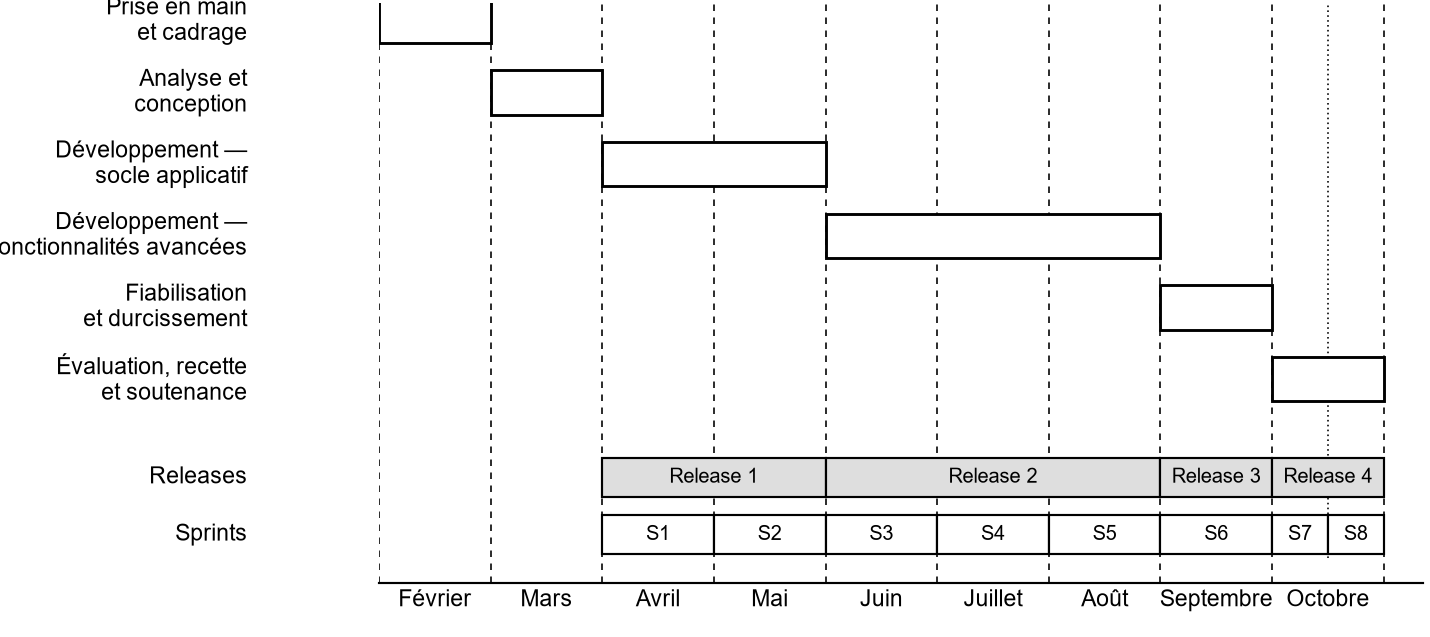
\includegraphics[width=0.98\linewidth, height=0.90\textheight, keepaspectratio]{fig1_1}
\caption{Diagramme de Gantt — Planification mensuelle des phases du projet}
\label{fig_1_1}
\end{figure}
\clearpage
\end{landscape}

\subsection{Découpage en sprints et en releases}
\label{sec_1_8_2}
Le développement, d’avril à octobre 2026, a été découpé en huit sprints : six d’environ quatre semaines, puis deux resserrés à deux semaines en octobre. Les deux premiers mois sont restés hors sprint — prise en main de l’environnement, analyse du besoin, conception UML. Chaque sprint se terminait par une revue avec l’encadrant (tableau~\ref{tab_1_3}).

Quatre releases agrègent ces sprints. Chacune correspond à un incrément complet du point de vue de l’utilisateur. La release 1 rend le cycle de candidature opérationnel, la 2 dote la plateforme de son aide à la décision, la 3 fiabilise l’ensemble et la 4 l’évalue avant la présentation finale.

% tableau 1.3
\setcounter{table}{2}
\begin{table}[!ht]
\centering
\caption{Découpage en sprints et en releases (avril – octobre 2026)}
\label{tab_1_3}
\renewcommand{\arraystretch}{1.25}\footnotesize
\setlength{\tabcolsep}{4pt}%
\begin{tabular}{|P{0.050\textwidth}|P{0.125\textwidth}|P{0.400\textwidth}|P{0.325\textwidth}|}
\hline
\textbf{Sprint} & \textbf{Période} & \textbf{Objectif du sprint} & \textbf{Critère validé en revue} \\
\hline
S1 & Avril 2026 & Mettre en place le socle technique : architecture back-end Spring Boot et front-end Angular, schéma PostgreSQL, authentification JWT et gestion des rôles & Les applications démarrent ensemble ; un compte par rôle se connecte et n’accède qu’à son périmètre \\
\hline
S2 & Mai 2026 & Cycle de base candidat–offre : publication et gestion des offres, dépôt de candidature avec CV, suivi de l’état du dossier & Une candidature est créée, déposée et suivie de bout en bout par le candidat et par le RH — clôture la release 1 \\
\hline
S3 & Juin 2026 & Présélection assistée : extraction du texte du CV, scoring sur 100 via l’API de Cohere, agents n8n et notifications e-mail & Un CV déposé est noté, la règle de décision appliquée et tracée dans le journal d’audit ; les notifications partent \\
\hline
S4 & Juillet 2026 & Pipeline RH/manager : planification des entretiens, retours structurés, avis du manager contresigné par le RH, tableau Kanban & Un dossier traverse présélection, entretiens et décision finale avec ses notifications \\
\hline
S5 & Août 2026 & Fonctions d’accompagnement : suggestions « Job idéal » (matching inverse), assistant conversationnel côté candidat, calendrier d’entretiens avec rappels & Les trois fonctions sont utilisables par un candidat et par un manager — clôture la release 2 \\
\hline
S6 & Septembre 2026 & Fiabilisation : tests fonctionnels de bout en bout, corrections de bugs et reprise des erreurs des agents d’automatisation, durcissement de la sécurité et de l’UX & Le scénario complet de démonstration s’exécute sans échec visible — clôture la release 3 \\
\hline
S7 & Octobre (1re quinzaine) & Évaluation du scoring : constitution du Gold Set de vingt CV, mesure à trois seuils, zone d’incertitude et réévaluation manuelle par le RH & Matrice de confusion et métriques produites, commentées puis intégrées au chapitre~4 \\
\hline
S8 & Octobre (2e quinzaine) & Recette finale et préparation de la soutenance : jeu de démonstration, enregistrement vidéo, relecture du rapport avec l’encadrant & Rapport et support de soutenance validés par l’encadrant entreprise — clôture la release 4 \\
\hline
\end{tabular}
\end{table}

\subsection{Backlog reconstitué des user stories}
\label{sec_1_8_3}
Le tableau~\ref{tab_1_4} rattache les user stories des principales fonctionnalités livrées à leur acteur bénéficiaire et à la release qui les a vues aboutir.

Backlog reconstitué après coup à partir du code livré et des démonstrations, non tenu en temps réel durant le stage ; les repères mensuels sont ceux de la macro-planification du tableau~\ref{tab_1_2} et n’ont donné lieu à aucune mesure de vélocité.

% tableau 1.4
\setcounter{table}{3}
\begin{table}[!ht]
\centering
\caption{Backlog reconstitué des user stories par release}
\label{tab_1_4}
\renewcommand{\arraystretch}{1.25}\footnotesize
\setlength{\tabcolsep}{4pt}%
\begin{tabular}{|P{0.430\textwidth}|P{0.140\textwidth}|P{0.375\textwidth}|}
\hline
\textbf{User story} & \textbf{Acteur bénéficiaire} & \textbf{Release (période 2026)} \\
\hline
Créer un compte et postuler à une offre (dépôt du CV) & Candidat & Release 1 — avril – mai \\
\hline
Suivre l’avancement de sa candidature à chaque étape & Candidat & Release 1 — avril – mai \\
\hline
Publier et gérer les offres d’emploi du périmètre RH & Responsable RH & Release 1 — avril – mai \\
\hline
Faire présélectionner les CV par un score IA paramétrable & Responsable RH & Release 2 — juin – août \\
\hline
Planifier les entretiens, émettre un avis et le contresigner & RH et Manager & Release 2 — juin – août \\
\hline
Consulter le tableau Kanban et le journal d’audit & Responsable RH & Release 2 — juin – août \\
\hline
Disposer d’un calendrier d’entretiens avec rappels & Manager & Release 2 — juin – août \\
\hline
Bénéficier des suggestions « Job idéal » et du chatbot & Candidat & Release 2 — juin – août \\
\hline
Exécuter un cycle complet sans régression visible & RH, Manager et Candidat & Release 3 — septembre \\
\hline
Évaluer, corriger et expliquer le scoring IA & Responsable RH & Release 4 — octobre \\
\hline
\end{tabular}
\end{table}
\section{Conclusion}
\label{sec_1_9}
Les limites du processus existant chez Sopra HR Software sont maintenant posées, tout comme la méthodologie suivie pendant le stage. Reste à entrer dans le vif du sujet : quels besoins précis JOB4YOU devait-il couvrir ? C’est l’objet du chapitre suivant.

        % ======== fin chap_01 ========
        \clearpage
        
        \jobFixLists{chap02}
        % ======== chap_02 ========
\chapter{Analyse et spécification des besoins}

Le contexte posé, restait à traduire la problématique en besoins concrets : qui utilise la plateforme, pour faire quoi, et avec quelles contraintes ? C’est ce que je détaille dans ce chapitre, acteur par acteur, avant de justifier les choix techniques préliminaires qui ont guidé l’architecture retenue.

\section{Introduction}
\label{sec_2_1}
Recueillir les besoins n’a rien eu d’un exercice ponctuel : cela s’est étalé sur les premières semaines du stage, au fil des échanges avec mon encadrant et de l’observation directe du processus RH. Ce qui suit est le résultat de cette phase, et sert de base directe à la conception présentée au chapitre suivant.

\section{Étude fonctionnelle}
\label{sec_2_2}
\subsection{Identification des acteurs du système}
\label{sec_2_2_1}
Cinq acteurs interviennent sur la plateforme JOB4YOU, chacun avec ses propres privilèges et fonctionnalités :

\begin{itemize}
\item Le Visiteur : utilisateur anonyme, non authentifié, qui consulte les offres d’emploi publiées et peut déposer son CV dans la fonctionnalité « Job idéal » pour obtenir des suggestions ; il doit créer un compte et s’authentifier pour soumettre une candidature.
\item Le Candidat : utilisateur authentifié disposant d’un compte (rôle ROLE\_USER), qui soumet ses candidatures, en suit l’avancement, échange avec l’assistant conversationnel et peut retirer un dossier tant qu’il n’est pas clos.
\item Le Responsable RH : acteur central du processus, il publie les offres, examine et valide les candidatures, fixe les entretiens, puis contresigne la décision — embauche ou refus. C’est à ce moment, et à lui seul, que le candidat reçoit une réponse.
\item Le Manager : son intervention commence dès que le dossier passe au statut « test technique ». Il ne voit que les candidatures de son périmètre, conduit les entretiens ou s’y associe, consigne un retour structuré puis propose un avis, favorable ou en refus ; le contreseing du RH reste nécessaire.
\item L’Administrateur : acteur transverse chargé de la gestion des comptes utilisateurs, des rôles, du paramétrage du scoring IA par famille de métier et de la supervision globale de la plateforme (journal d’audit).
\end{itemize}

Le tableau~\ref{tab_2_1} précise, action par action, les rôles habilités — une répartition qui correspond exactement aux règles d’autorisation implémentées côté back-end.

% tableau 2.1
\setcounter{table}{0}
\begin{table}[!ht]
\centering
\caption{Matrice des responsabilités par rôle}
\label{tab_2_1}
\renewcommand{\arraystretch}{1.25}\footnotesize
\setlength{\tabcolsep}{4pt}%
\begin{tabular}{|P{0.441\textwidth}|P{0.093\textwidth}|P{0.104\textwidth}|P{0.181\textwidth}|P{0.093\textwidth}|}
\hline
\textbf{Action} & \textbf{RH} & \textbf{Manager} & \textbf{Administrateur} & \textbf{Candidat} \\
\hline
Publier / gérer une offre d’emploi & Oui & Non & Oui & Non \\
\hline
Valider un CV (passage CV\_REVIEWED) & Oui & Non & Oui & Non \\
\hline
Planifier un entretien & Oui & Oui (son périmètre) & Oui & Non \\
\hline
Saisir un retour d’évaluation & Oui & Oui & Oui & Non \\
\hline
Valider / transmettre un retour au candidat & Oui & Non & Oui & Non \\
\hline
Avis sur la candidature (favorable / refus proposé) & Oui & Oui (son périmètre) & Oui & Non \\
\hline
Décision finale contresignée (« retenu » / « refusé ») & Oui & Non & Oui & Non \\
\hline
Gérer les utilisateurs et les rôles & Non & Non & Oui & Non \\
\hline
Paramétrer le scoring IA & Non & Non & Oui & Non \\
\hline
Consulter le journal d’audit & Oui & Non & Oui & Non \\
\hline
\end{tabular}
\end{table}
J’ai volontairement donné au RH et à l’Administrateur la main sur tout le cycle : ils enregistrent un avis comme le ferait le manager et sont seuls à contresigner la décision finale. Un compte purement manager ne peut écrire ni l’embauche ni un statut du pipeline. L’auteur de chaque décision reste dans le journal d’audit.

\subsection{Identification des besoins fonctionnels}
\label{sec_2_2_2}
Les échanges avec mon encadrant entreprise et l’étude de l’existant ont fait émerger les besoins fonctionnels suivants :

\begin{itemize}
\item Authentification et gestion des sessions sécurisée par jeton JWT, avec gestion différenciée des accès selon le rôle de l’utilisateur.
\item Gestion des offres d’emploi : création, modification, publication, clôture et expiration automatique des offres dont la date limite est dépassée.
\item Gestion des candidatures : soumission en ligne avec dépôt de CV, consultation, filtrage et suivi de l’état d’avancement de chaque dossier.
\item Analyse automatique des candidatures par intelligence artificielle : extraction du contenu du CV et calcul d’un score de pertinence (technique, communication, adéquation séniorité) avec possibilité de correction manuelle par le RH.
\item Gestion des entretiens : planification, changement de statut (planifié, en cours, terminé, annulé, reprogrammé), envoi d’invitations et de rappels automatiques.
\item Gestion des retours d’évaluation : saisie par le manager après l’entretien, validation par le RH et notification au candidat.
\item Décision à deux niveaux : l’avis du manager, favorable ou en refus, ne prend valeur que contresignée par le RH ou l’Administrateur. La décision prend alors l’une des deux formes : une embauche datée pour la présentation des documents, ou un refus motivé. Un garde-fou interdit toute décision sur un dossier non validé par le RH, comme toute validation finale par un compte purement manager.
\item Notifications automatiques par e-mail à chaque étape clé (confirmation de candidature, invitation à un entretien, décision finale) ; l’e-mail de décision finale n’est adressé au candidat qu’après le contreseing du RH, l’avis du manager notifiant le RH ; seule exception, le refus prononcé par l’agent IA, notifié dès l’écartement d’office et qui n’est pas doublé lorsque le RH se borne à le confirmer.
\item Tableau de pilotage visuel de type Kanban permettant de visualiser en un coup d’œil la répartition des candidatures par statut.
\item Gestion des utilisateurs, des rôles et paramétrage des profils de pondération du score IA par famille de métier.
\item Matching inverse (« Job idéal ») : un visiteur peut déposer son CV sans postuler à une offre précise ; le système le compare aux offres actives et lui suggère les plus pertinentes avec un score de compatibilité.
\end{itemize}

\subsection{Identification des besoins non fonctionnels}
\label{sec_2_2_3}
Au-delà des fonctionnalités métier, la plateforme doit aussi répondre aux exigences non fonctionnelles suivantes :

\begin{itemize}
\item Sécurité : authentification robuste par jeton JWT signé d’une durée de vie de 24 heures, hachage des mots de passe avec BCrypt, contrôle d’accès basé sur les rôles (RBAC) appliqué à la fois côté front-end et côté back-end, jeton de réinitialisation de mot de passe valable 15 minutes et limitation du nombre de tentatives de connexion.
\item Performance : temps de réponse cible inférieur à 500 ms pour les opérations de lecture courantes et inférieur à 2 s pour les opérations d’écriture, chargement asynchrone des traitements longs (scoring IA, envoi d’e-mails) afin de ne pas bloquer l’utilisateur, et taille maximale des CV déposés fixée à 10 Mo côté serveur (formats PDF, DOC, DOCX), le formulaire de candidature refusant déjà les fichiers de plus de 5 Mo. Cette différence de plafond est volontaire : la validation du formulaire est un confort offert à l’utilisateur, la limite serveur est la véritable barrière de sécurité, seule opposée à un client qui contournerait l’interface.
\item Ergonomie et responsive design : interface claire, intuitive et utilisable aussi bien sur poste de travail que sur tablette.
\item Fiabilité : garde-fous métier empêchant les transitions de statut incohérentes (ex. acceptation avant l’entretien téléphonique RH, validation finale sans avis manager en attente, embauche sans date de présentation des documents, entretien planifié sur un dossier clos).
\item Maintenabilité et évolutivité : architecture modulaire en couches, séparation claire entre front-end, back-end et automatisation, facilitant l’ajout de nouvelles fonctionnalités.
\item Traçabilité : journalisation des actions sensibles (changements de statut, corrections de score) dans un journal d’audit.
\end{itemize}

\subsection{Diagramme d’activité — Vue d’ensemble du processus de recrutement}
\label{sec_2_2_4}
Avant de détailler les fonctionnalités attendues, ce diagramme d’activité pose le flux métier global. Il décrit l’enchaînement des activités du recrutement, de la publication de l’offre jusqu’à la décision finale, et les acteurs qui les portent, indépendamment de toute considération technique.

Le diagramme d’activité, présenté en trois volets (figures~\ref{fig_2_1a}, \ref{fig_2_1b} et \ref{fig_2_1c}), rend explicite un point que le texte laissait dans l’ombre. L’entretien téléphonique RH est un passage obligé avant toute évaluation technique (section~\ref{sec_4_5_8}). La transmission au manager désigné par le RH (section~\ref{sec_3_5_4}) n’intervient qu’à ce moment-là, pas dès la validation du CV, conformément à la correction décrite en section~\ref{sec_4_5_5}.

Le rejet automatique par l’IA n’est pas une fin de parcours : il rejoint l’étape commune de notification et de journalisation, comme le contreseing du RH. Deux issues humaines le suivent (figure~\ref{fig_3_8}) : le RH confirme le refus, ou le conteste par une correction de score au-dessus du seuil.

Le volet~\ref{fig_2_1a} couvre le dépôt et la présélection automatisée, le volet~\ref{fig_2_1b} la suite côté RH et manager, le volet~\ref{fig_2_1c} la décision finale et sa notification. En une seule figure, le texte tombait à 5,4 pt imprimés ; là, il reste entre 9,3 et 11,2 pt.

% figure 2.1a / 2.1b / 2.1c
% La vue d'ensemble tenait dans une seule figure paysage (fig2_1.png,
% 2221x1383 px) : ramenee a 0,98\linewidth x 0,90\textheight en paysage, elle
% n'imprimait plus ses etiquettes qu'a 5,4 pt, sous le plancher de 8 pt retenu
% pour ce rapport. Elle est donc decompee en trois volets enchaunes, chacun
% rendu a sa propre echelle : 8,7 pt imprimes pour 2.1a (paysage, ratio 2,3),
% 12,8 pt pour 2.1b (portrait) et 10,2 pt pour 2.1c (portrait). Les numeros a
% suffixe alphabetique suivent le procede deja utilise pour 3.2a/3.2b et
% 4.15a/4.15b, ce qui ne decale aucune figure du chapitre.
\setcounter{figure}{0}
\begingroup\renewcommand{\thefigure}{2.1a}
\begin{landscape}
\pagestyle{lscape}
\begin{figure}[p]
\centering
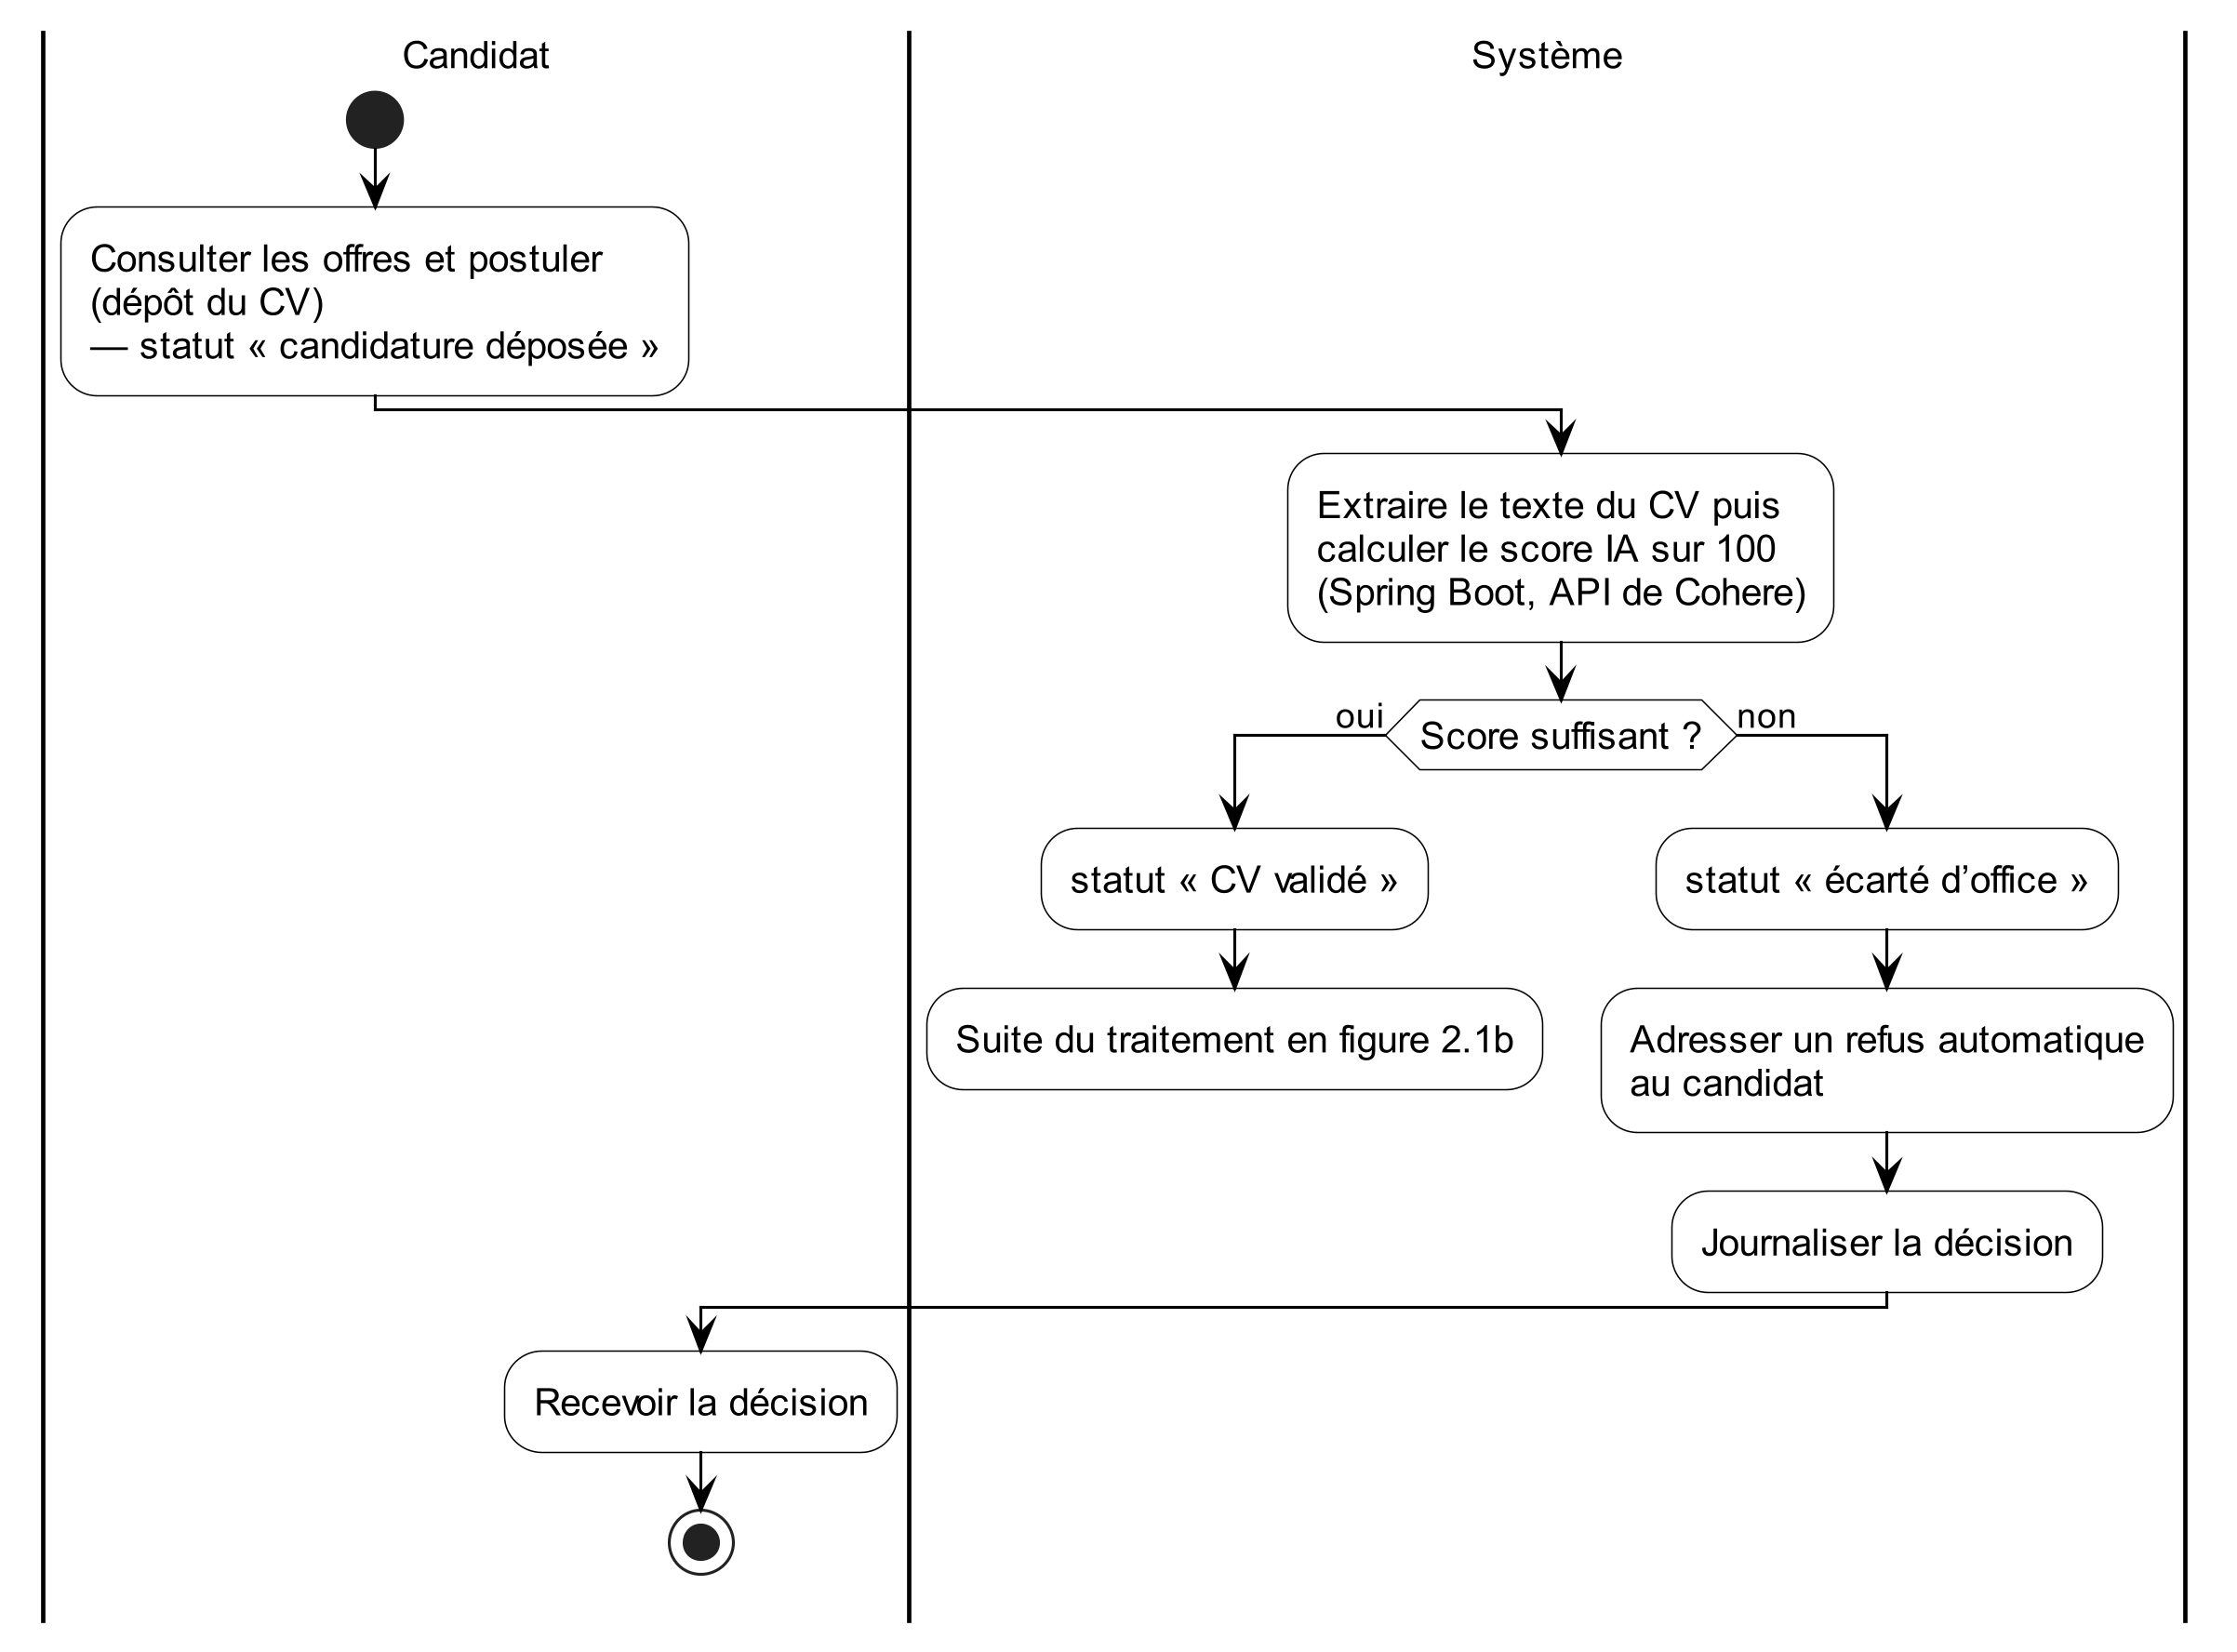
\includegraphics[width=0.98\linewidth, height=0.92\textheight, keepaspectratio]{fig2_1a}
\caption{Diagramme d’activité — Dépôt de la candidature et présélection automatisée par le score IA}
\label{fig_2_1a}
\end{figure}
\clearpage
\end{landscape}
\endgroup

\setcounter{figure}{0}
\begingroup\renewcommand{\thefigure}{2.1b}
\begin{figure}[!ht]
\centering
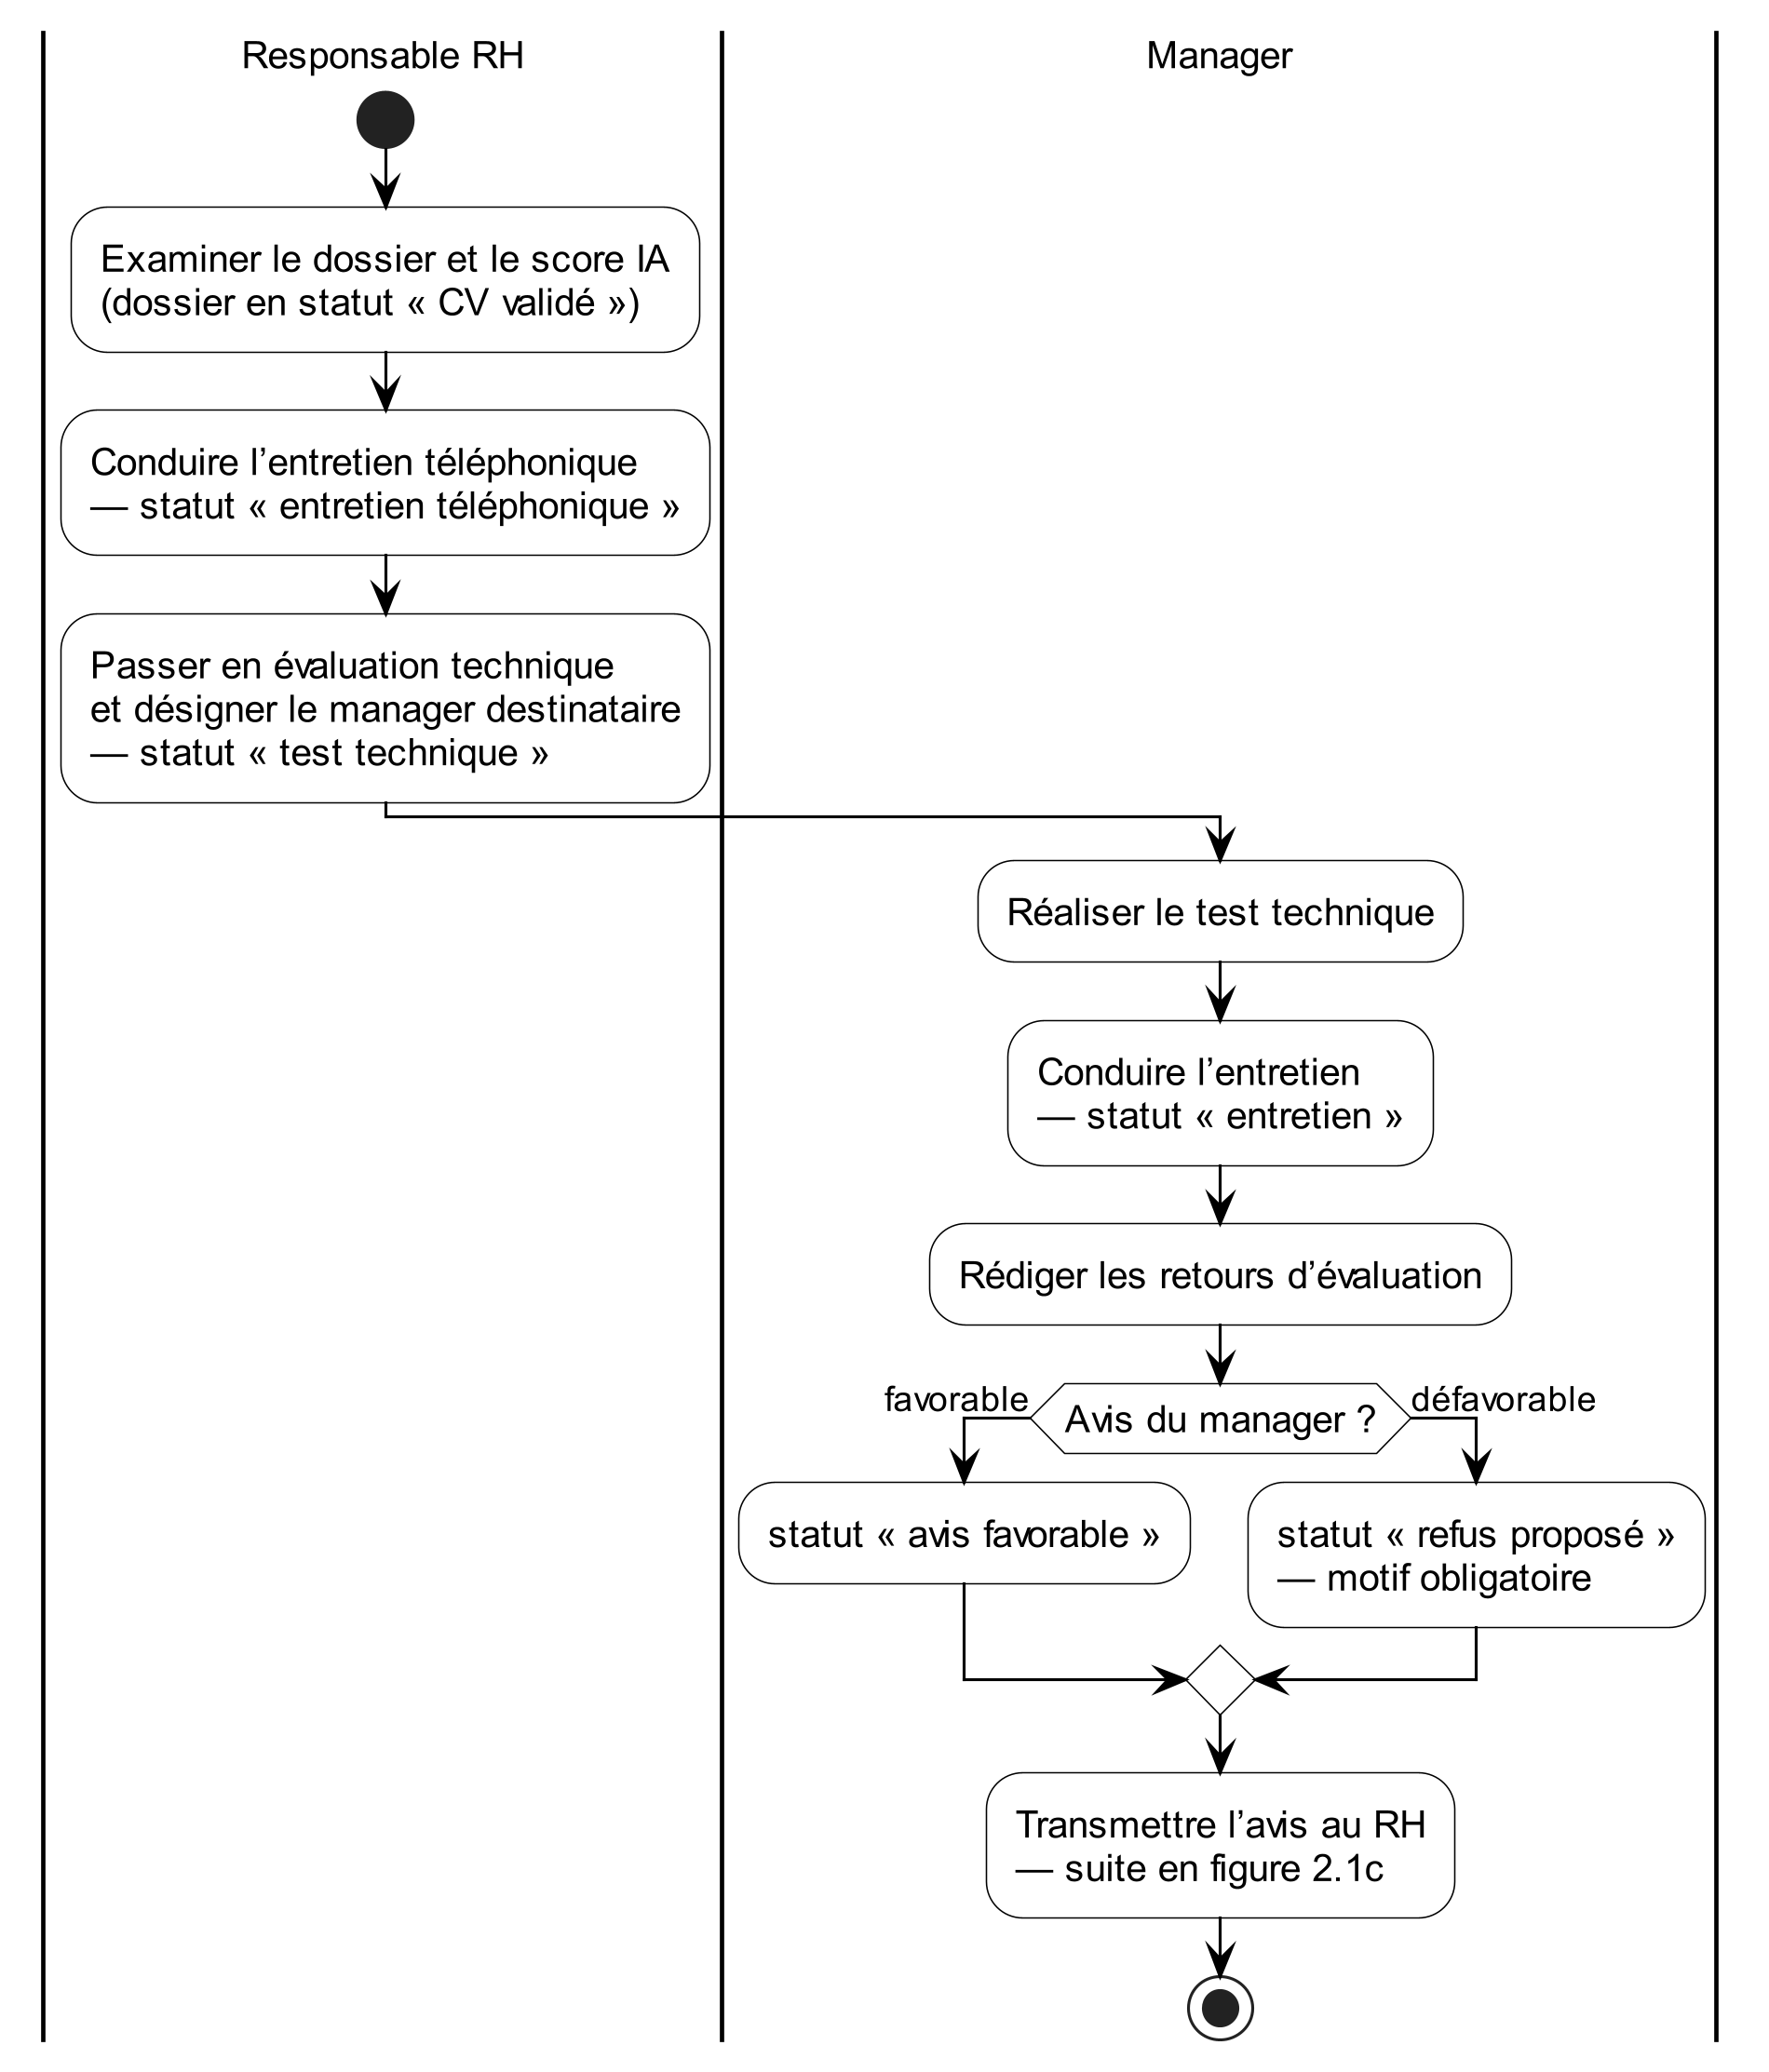
\includegraphics[width=\linewidth, height=0.94\textheight, keepaspectratio]{fig2_1b}
\caption{Diagramme d’activité — Traitement du dossier par le RH et le manager, jusqu’à l’avis du manager}
\label{fig_2_1b}
\end{figure}
\endgroup

\setcounter{figure}{0}
\begingroup\renewcommand{\thefigure}{2.1c}
\begin{landscape}
\pagestyle{lscape}
\begin{figure}[p]
\centering
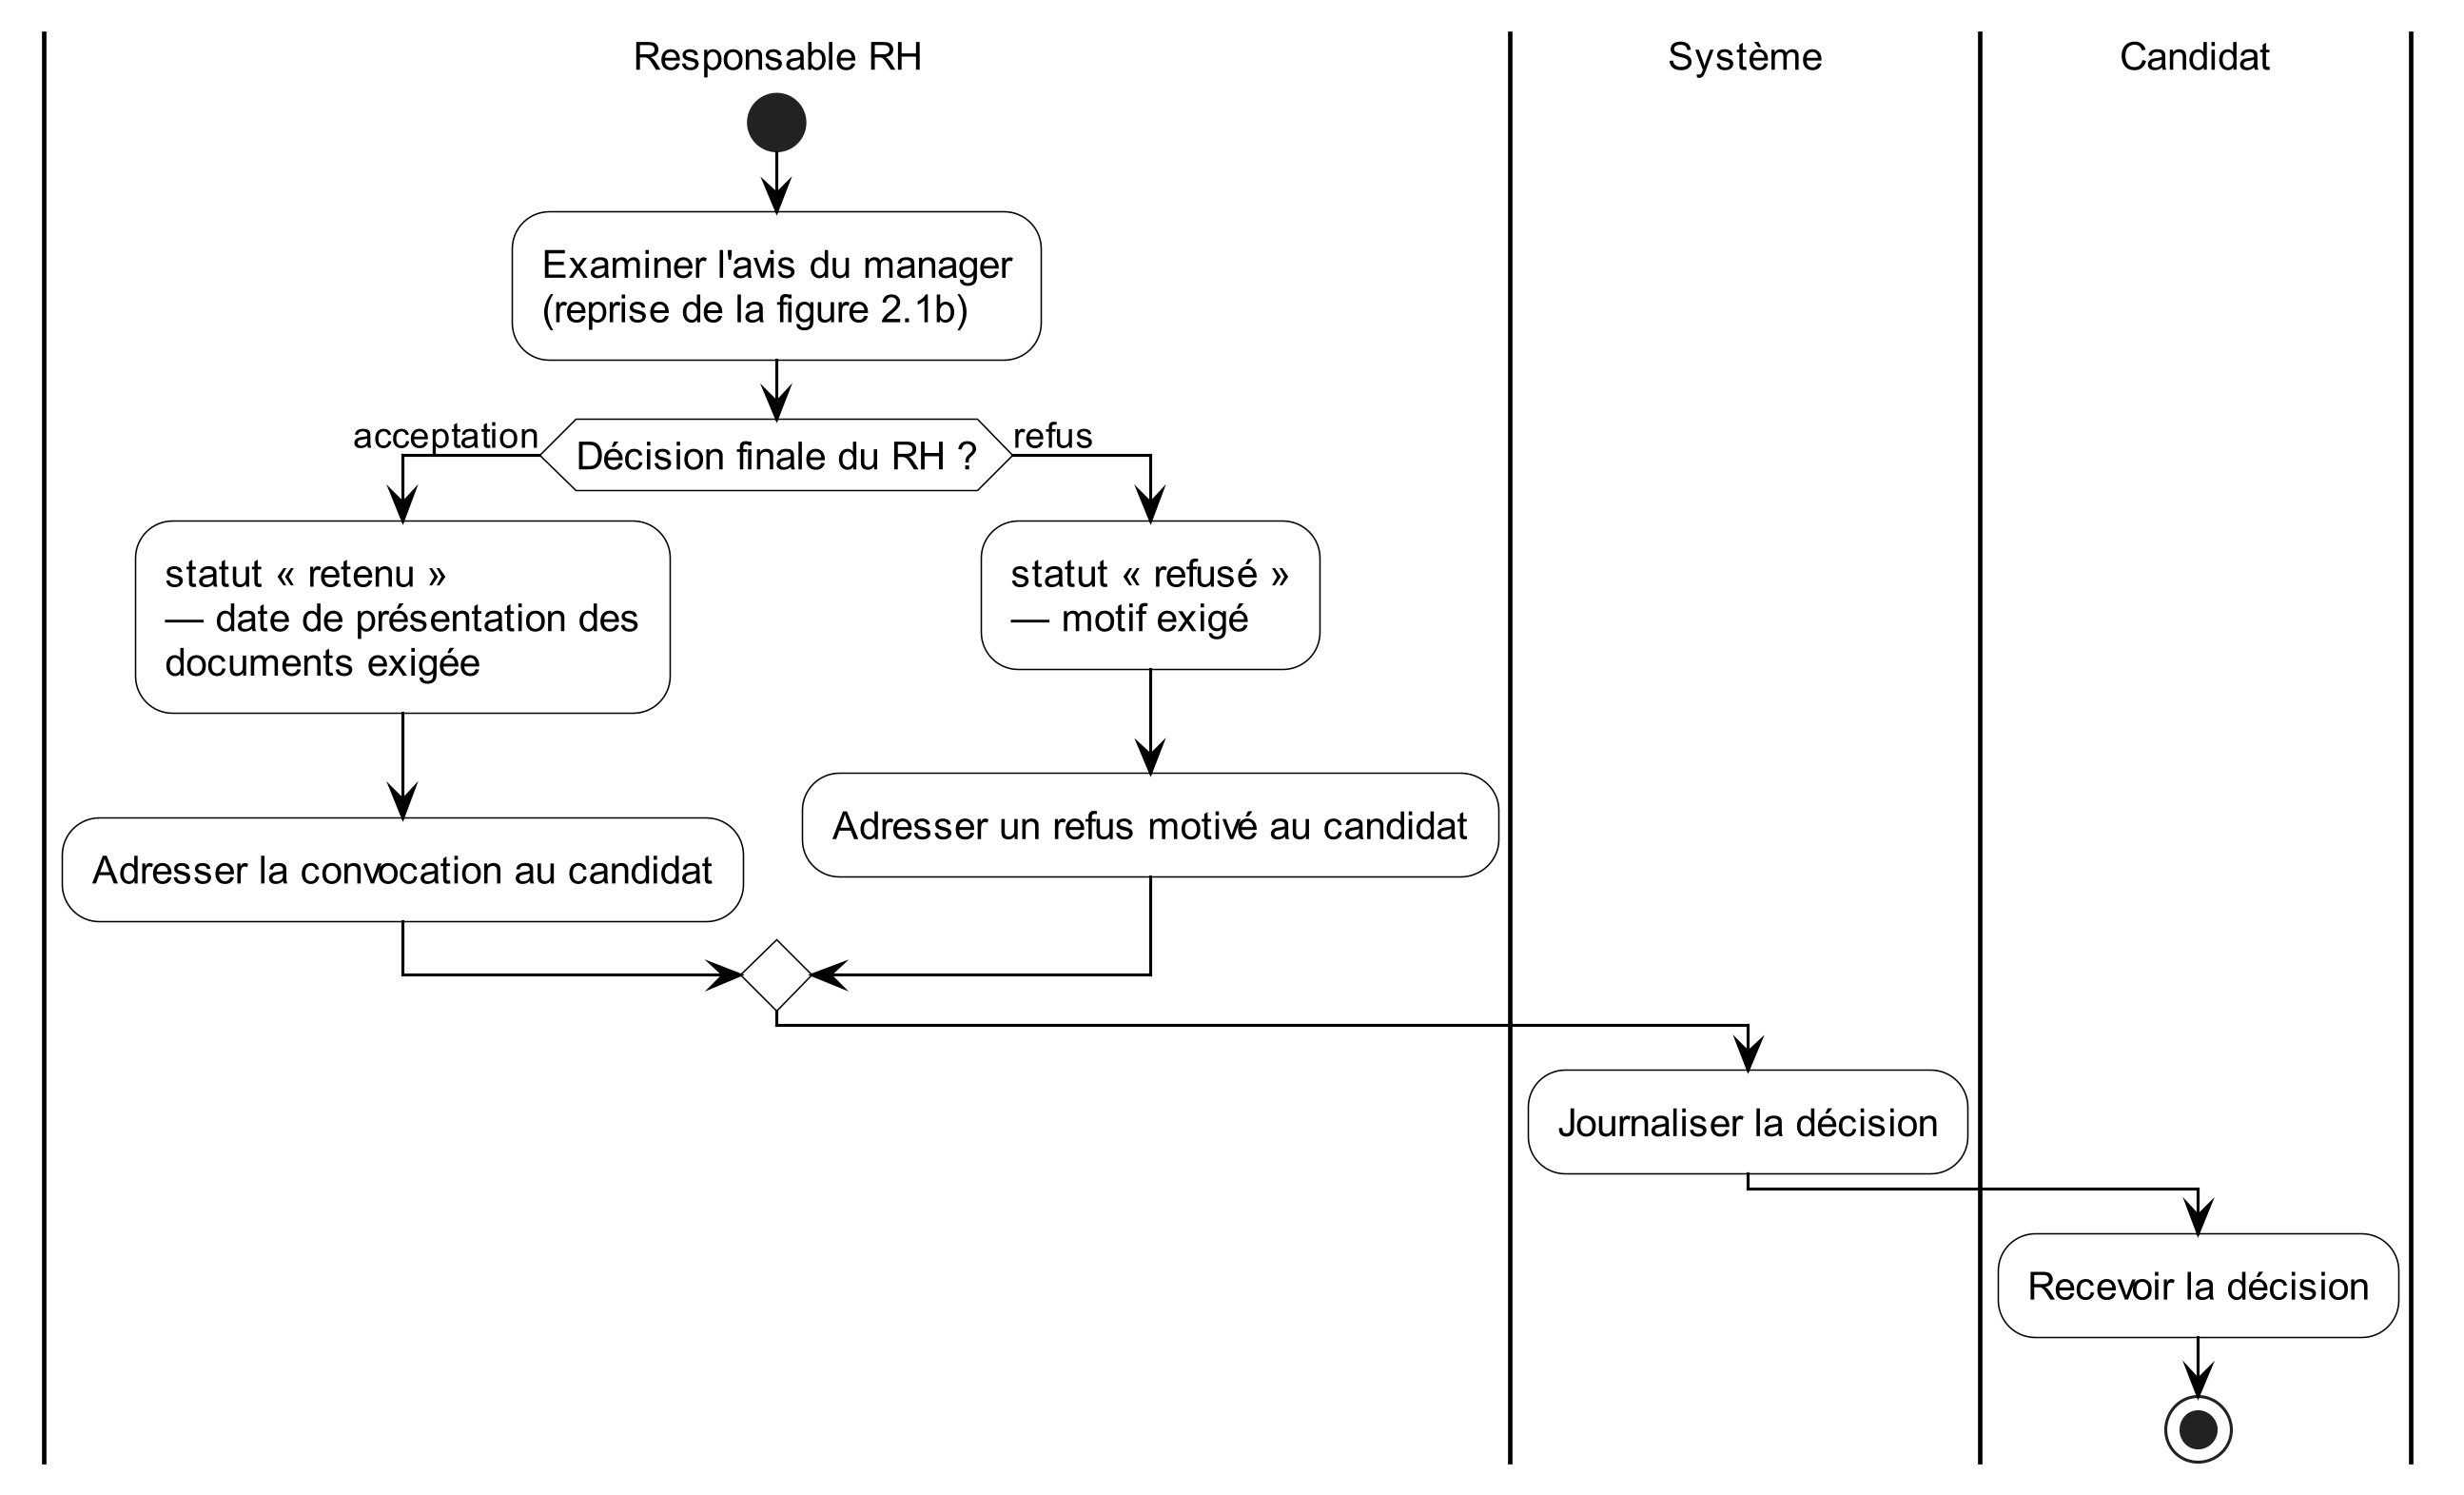
\includegraphics[width=0.98\linewidth, height=0.92\textheight, keepaspectratio]{fig2_1c}
\caption{Diagramme d’activité — Décision finale du RH, journalisation et notification du candidat}
\label{fig_2_1c}
\end{figure}
\clearpage
\end{landscape}
\endgroup

\subsection{Diagrammes de cas d’utilisation}
\label{sec_2_2_5}
Le périmètre fonctionnel est présenté en trois vues, une par module : portail candidat (figure~\ref{fig_2_3}), recrutement et évaluation (figure~\ref{fig_2_4}), administration (figure~\ref{fig_2_5}). Chaque vue est enfermée dans la limite du système «~JOB4YOU~». Deux relations seulement sont tracées : l’acteur à son cas, et le lien «~include~» entre deux cas.

L’authentification est représentée par un cas unique « S’authentifier », rattaché par une relation d’inclusion aux cas qui la supposent ; la flèche part du cas principal vers le cas inclus, conformément à la norme UML \cite{ref03}.

Le visiteur conserve la consultation des offres et les suggestions « Job idéal » ; le candidat authentifié y ajoute le dépôt de candidature, le suivi de son dossier, l’accès à ses entretiens et l’assistant conversationnel. Les autorisations sont contrôlées côté serveur selon le rôle et le périmètre métier.

Les figures ne montrent que les cas principaux : le tableau~\ref{tab_2_1} fait foi pour le détail des droits. L’administrateur peut aussi publier une offre, planifier, émettre un avis et contresigner ; le RH saisit un retour d’évaluation et consulte le journal d’audit.
La première vue couvre le portail public et le domaine candidat : consultation des offres, suggestions « Job idéal », dépôt de candidature et suivi en libre-service (figure~\ref{fig_2_3}).

% figure 2.3 : seule figure du chapitre 2 a relever du vrai paysage
\setcounter{figure}{1}
\begin{landscape}
\pagestyle{lscape}
\begin{figure}[p]
\centering
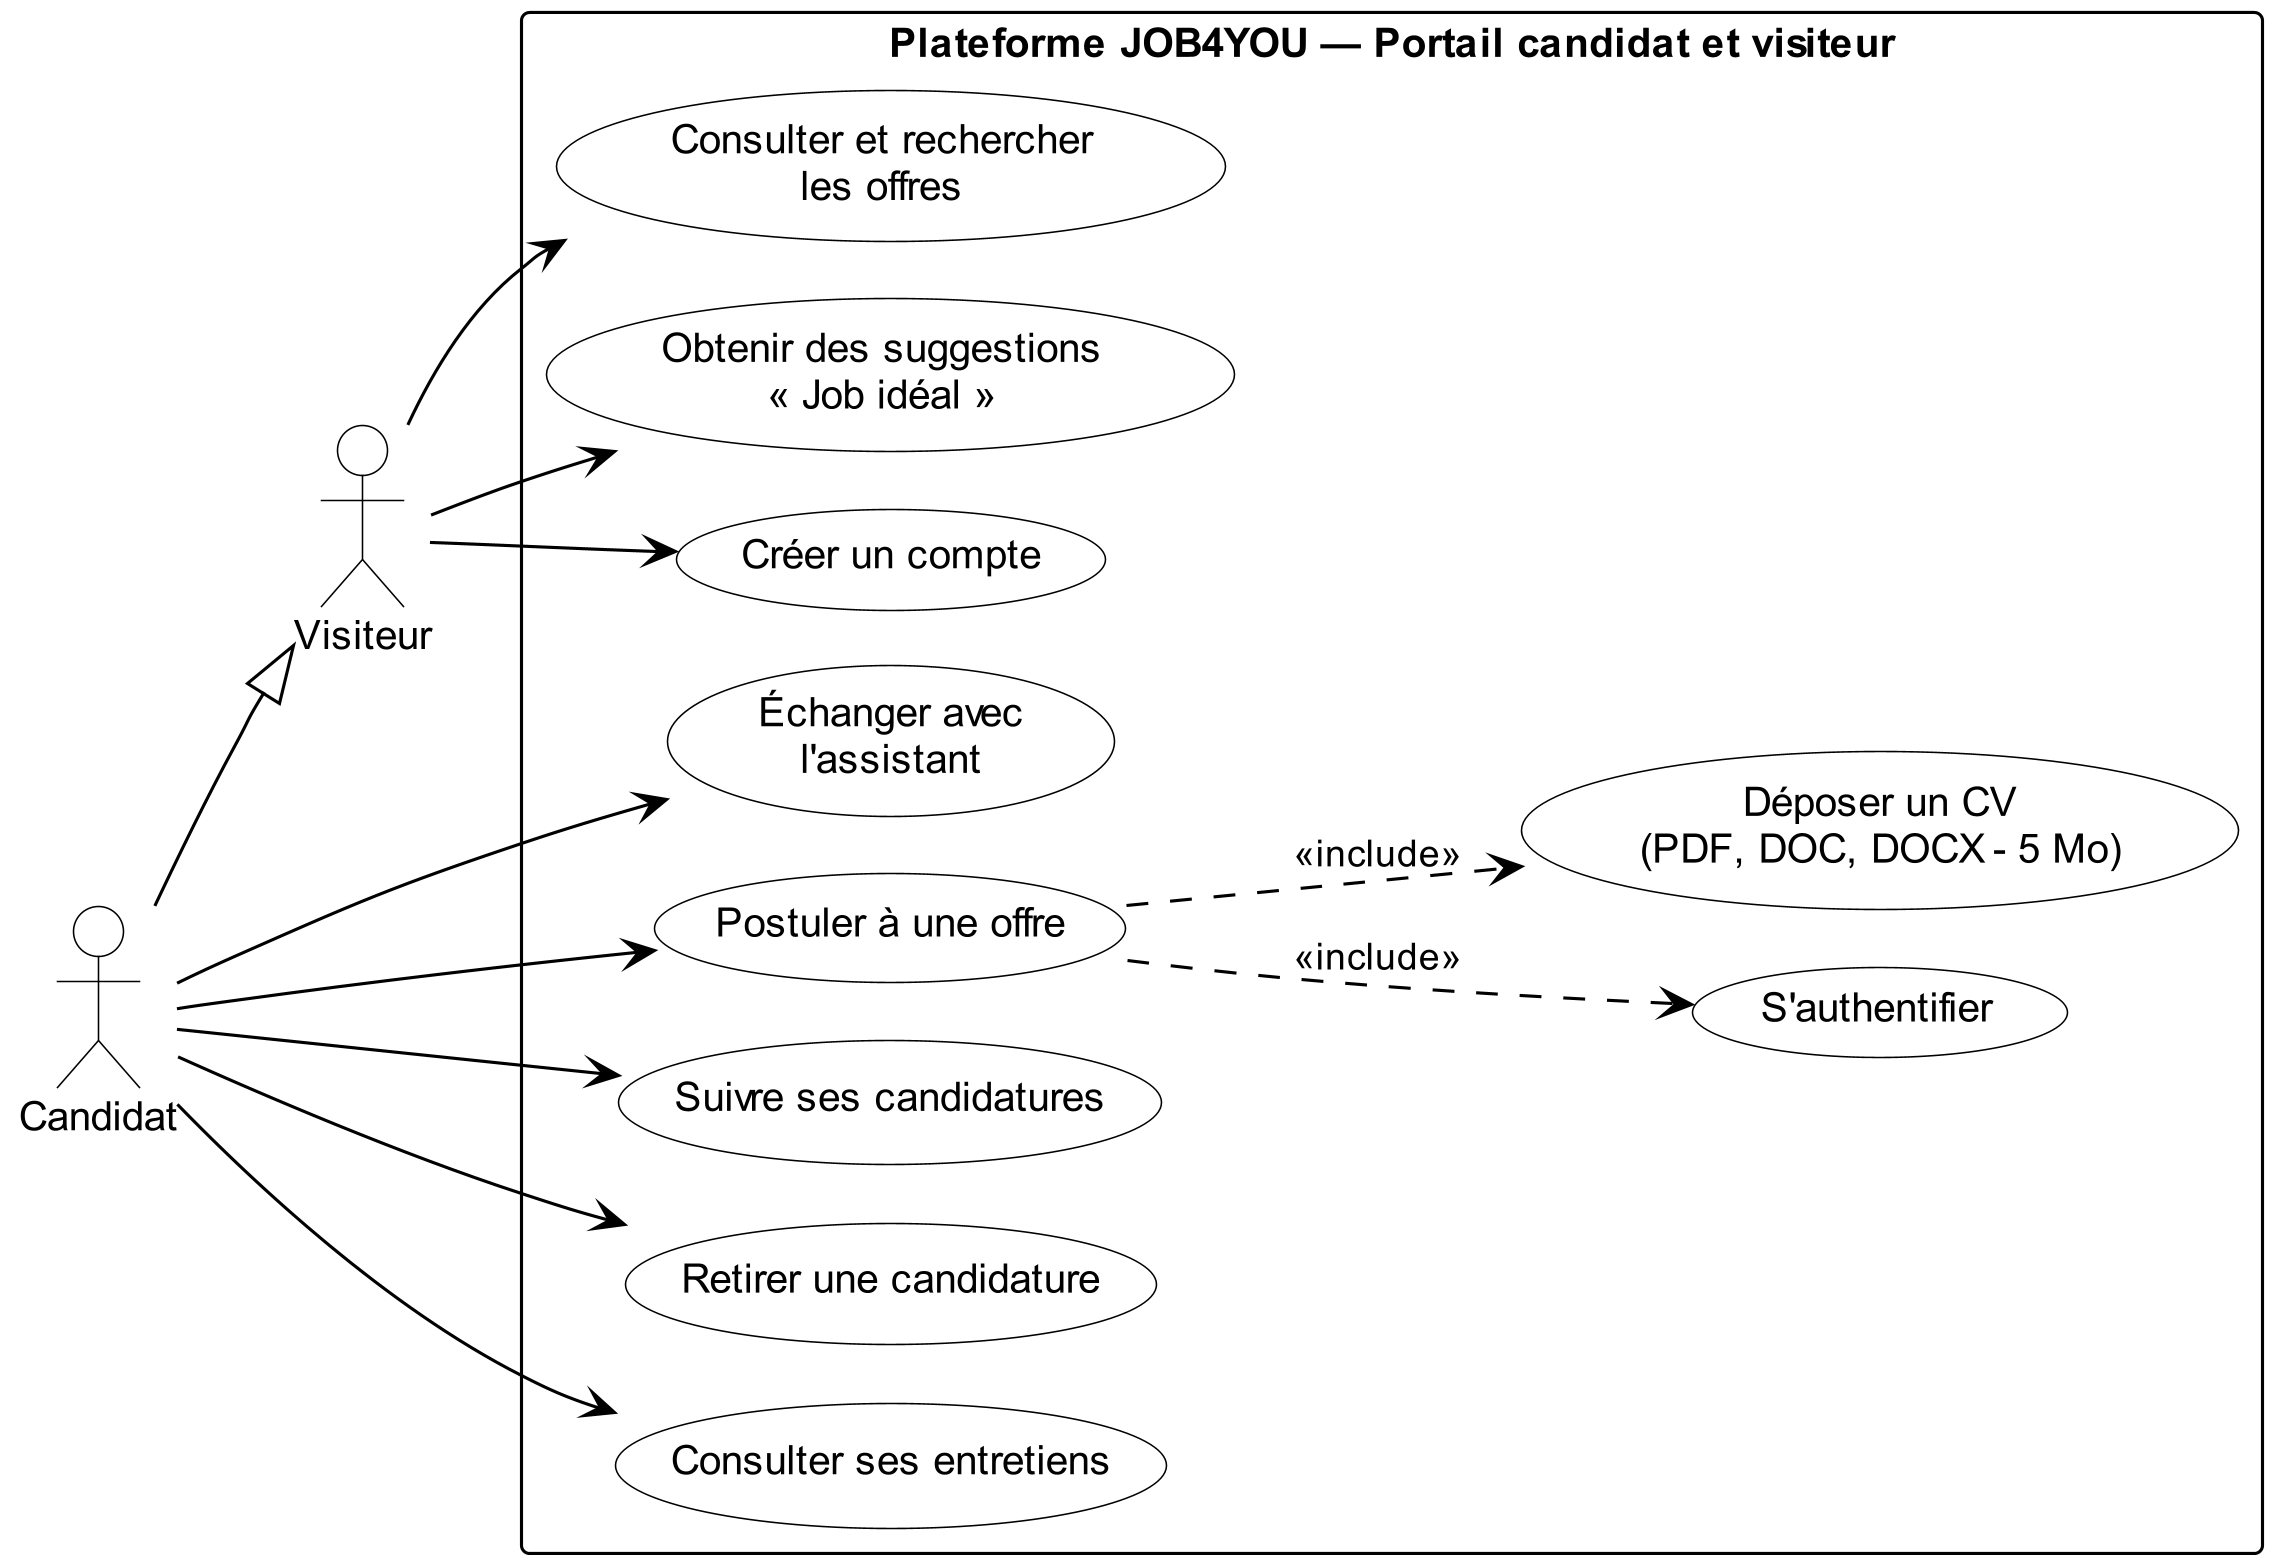
\includegraphics[width=0.98\linewidth, height=0.92\textheight, keepaspectratio]{fig2_3}
\caption{Diagramme de cas d’utilisation — Portail candidat et visiteur}
\label{fig_2_3}
\end{figure}
\clearpage
\end{landscape}

Le deuxième zoom décrit le cœur du processus côté RH et manager : publication des offres, filtrage, entretiens, retours d’évaluation, avis du manager puis contreseing RH de la décision finale (figure~\ref{fig_2_4}). L’envoi des notifications par e-mail y est modélisé comme un cas inclus, déclenché par la planification ou par la décision, et non comme un cas autonome.

% figure 2.4
\setcounter{figure}{2}
\begin{figure}[!ht]
\centering
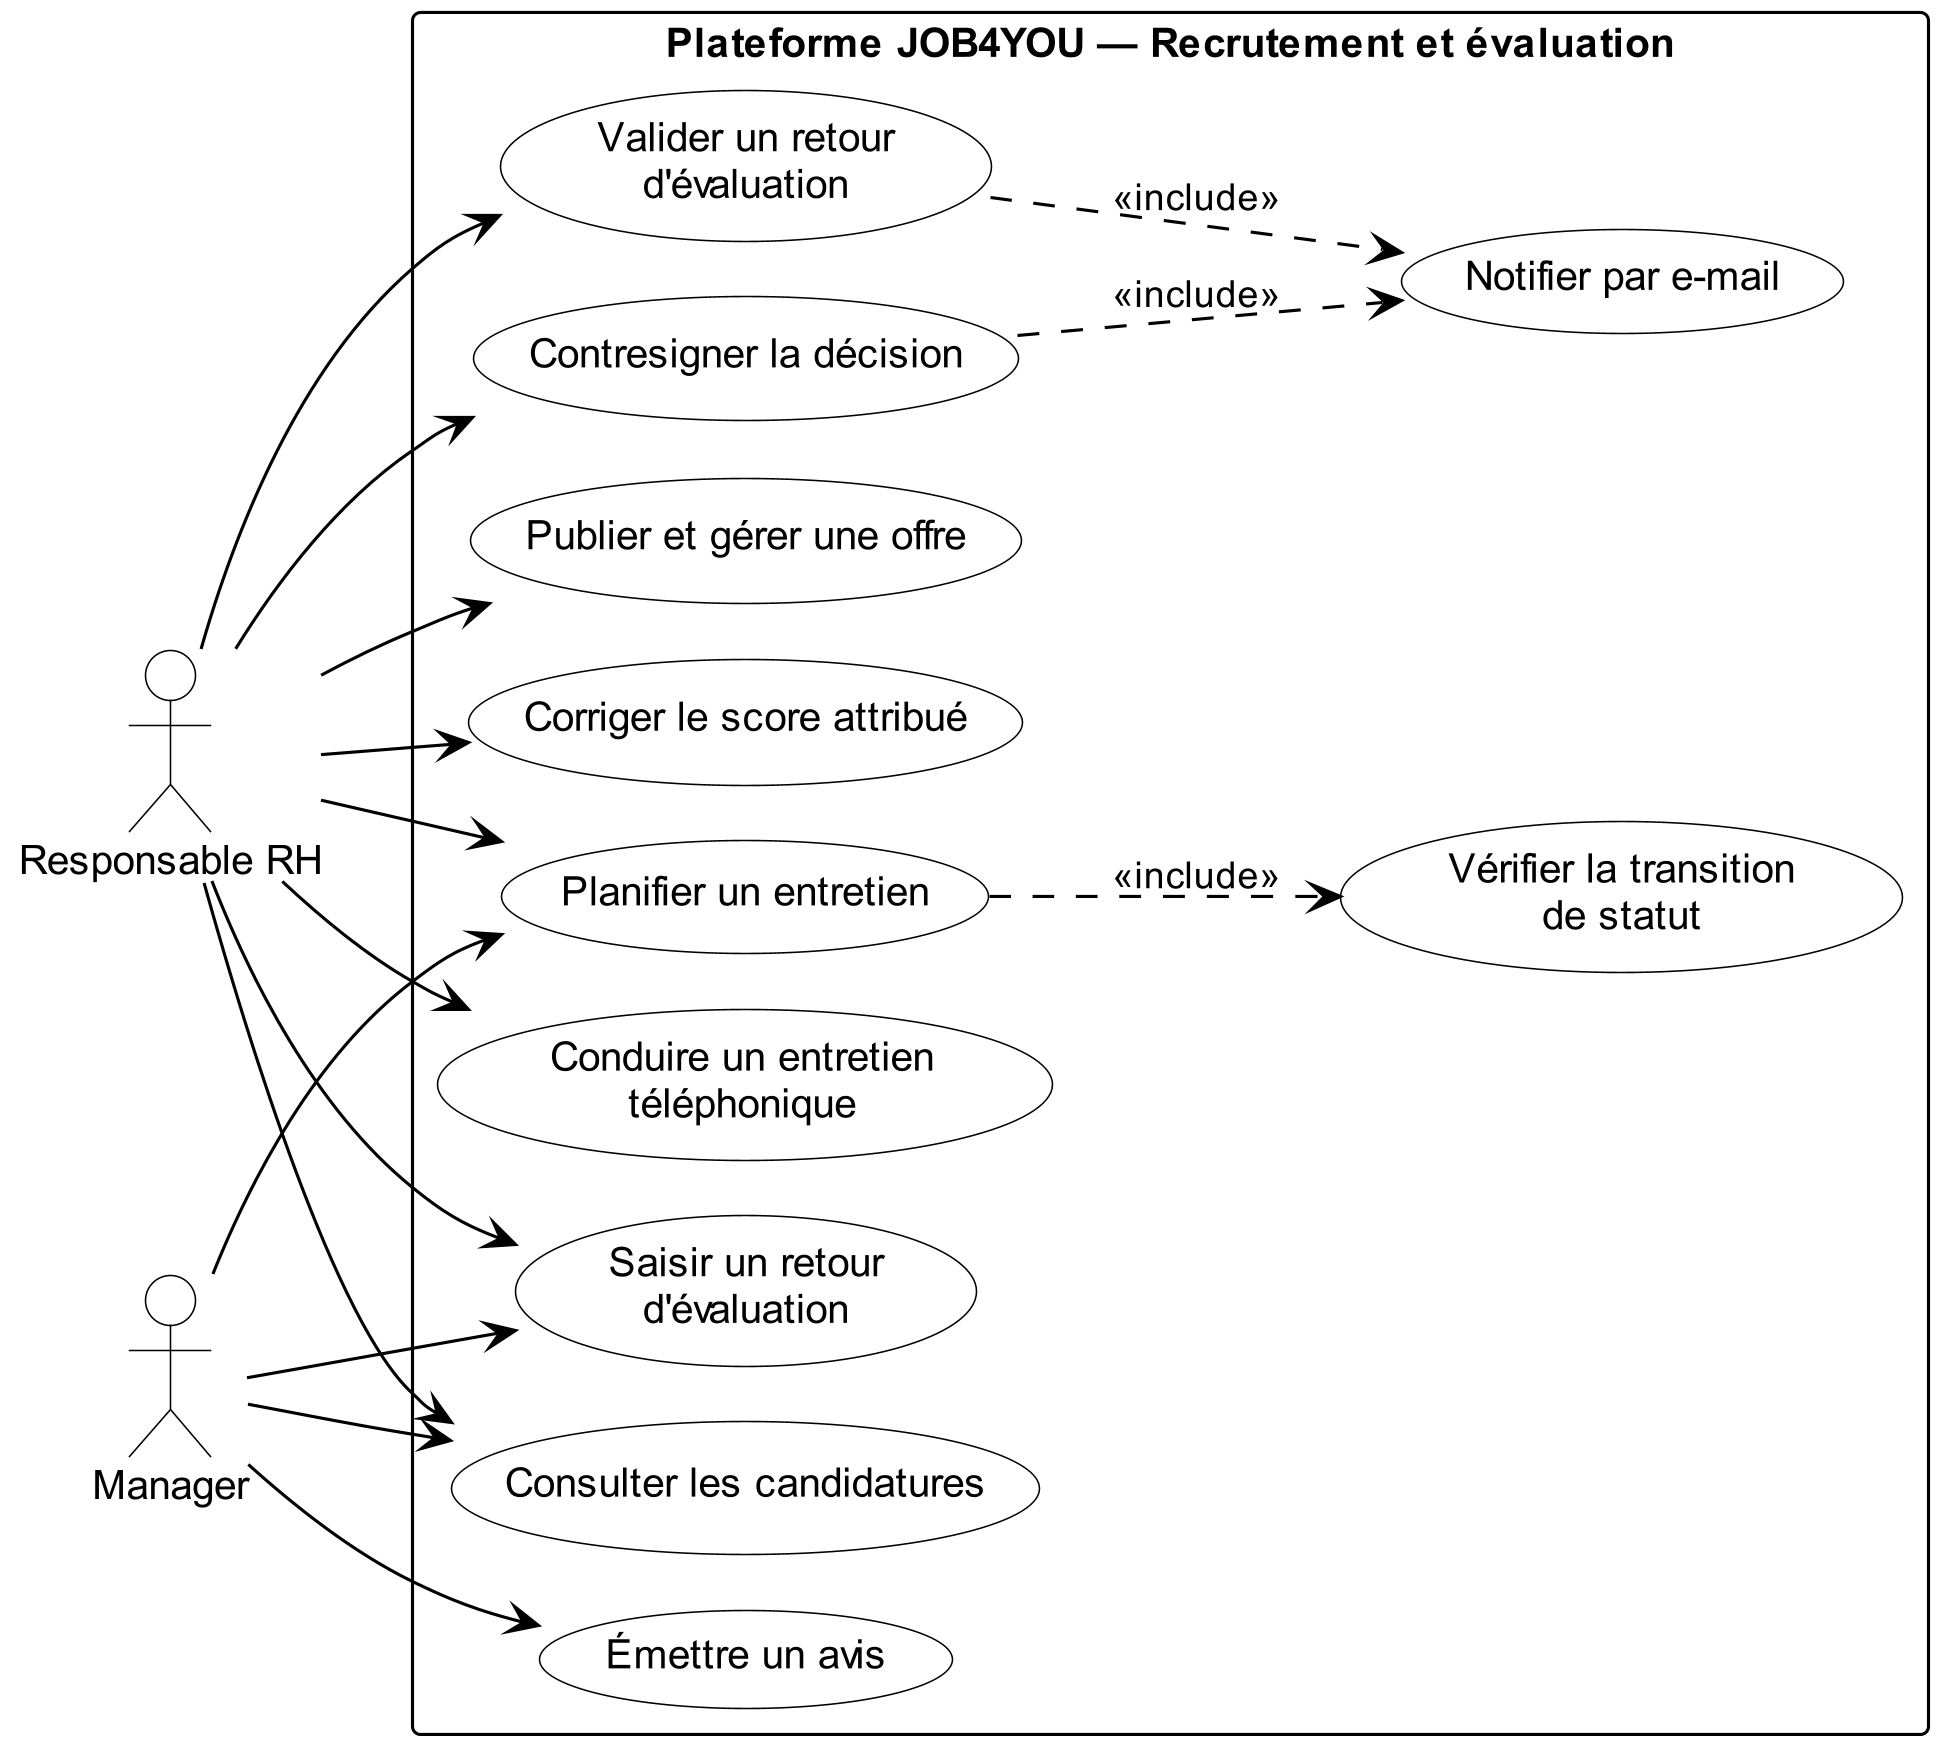
\includegraphics[width=\linewidth, height=0.94\textheight, keepaspectratio]{fig2_4}
\caption{Diagramme de cas d’utilisation — Recrutement et évaluation}
\label{fig_2_4}
\end{figure}

Le troisième zoom isole le périmètre d’administration : comptes et rôles, rattachement d’un utilisateur à un département ou à une famille de métier, pondérations du scoring IA et journal d’audit (figure~\ref{fig_2_5}). Le référentiel lui-même n’est pas administrable : les départements sont créés au démarrage et exposés en lecture seule, les familles de métier sont un énuméré figé dans le code.

% figure 2.5
\setcounter{figure}{3}
\begin{figure}[!ht]
\centering
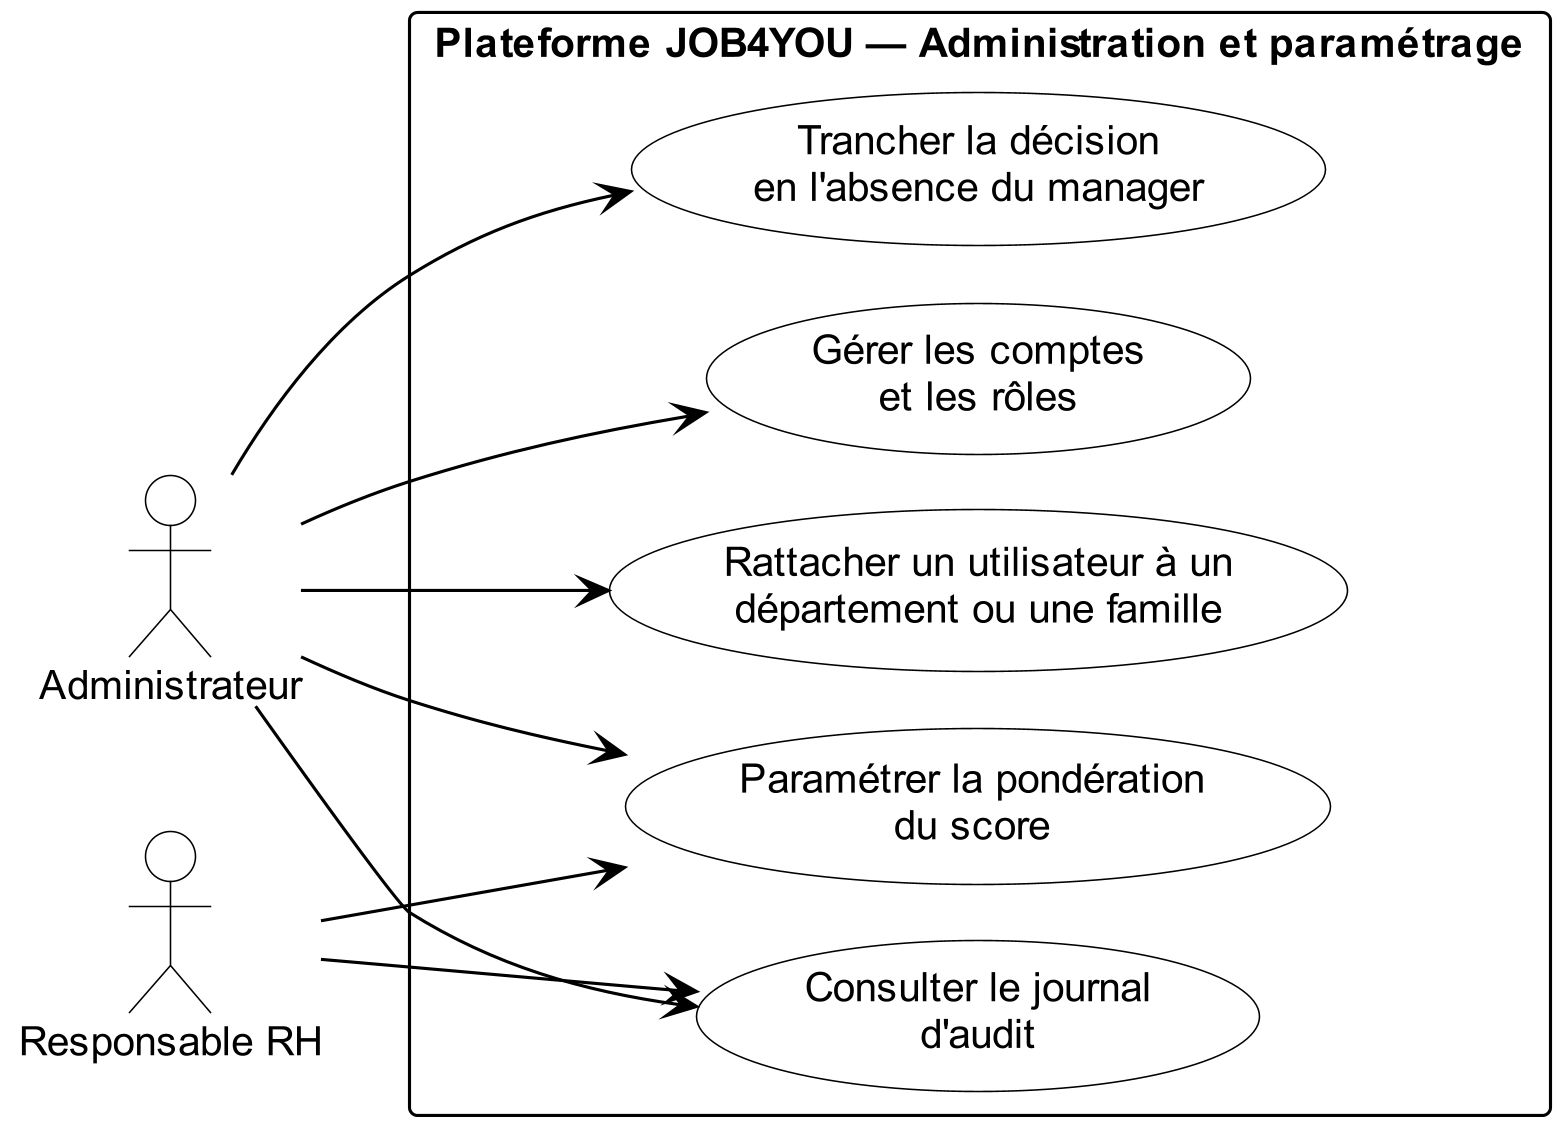
\includegraphics[width=\linewidth, height=0.94\textheight, keepaspectratio]{fig2_5}
\caption{Diagramme de cas d’utilisation — Administration et paramétrage}
\label{fig_2_5}
\end{figure}

\subsection{Description textuelle de quelques cas d’utilisation}
\label{sec_2_2_6}
Le tableau~\ref{tab_2_2} détaille le scénario nominal de deux cas d’utilisation représentatifs du processus métier.

% tableau 2.2
\setcounter{table}{1}
\begin{table}[!ht]
\centering
\caption{Description textuelle de deux cas d’utilisation représentatifs}
\label{tab_2_2}
\renewcommand{\arraystretch}{1.25}\footnotesize
\setlength{\tabcolsep}{4pt}%
\begin{tabular}{|P{0.137\textwidth}|P{0.271\textwidth}|P{0.538\textwidth}|}
\hline
\textbf{Élément} & \textbf{Cas d’utilisation « Postuler à une offre »} & \textbf{Cas d’utilisation « Avis manager, puis décision finale »} \\
\hline
Acteur principal & Candidat & Manager (avis), puis Responsable RH (contreseing) \\
\hline
Pré-condition & L’offre est publiée & Le dossier a été transmis au manager pour évaluation technique : un avis favorable comme un refus proposé sont admis sur les seuls statuts « test technique », « entretien » et « entretien final », c’est-à-dire après le pré-filtrage téléphonique du RH. \\
\hline
Scénario nominal & Le candidat consulte l’offre, remplit le formulaire de candidature et dépose son CV. Le système enregistre la candidature, envoie un e-mail de confirmation et déclenche l’analyse IA du CV. & Le manager consulte le dossier du candidat, ses scores et ses éventuels retours, puis émet un avis — favorable, ou refus proposé accompagné d’un motif. Le RH, averti par e-mail et dans sa liste de candidats, contresigne cet avis : « retenu » avec date de présentation des documents, ou « refusé » motivé. \\
\hline
Post-condition & La candidature est créée avec le statut « candidature déposée », puis mise à jour automatiquement selon le score. & L’avis est enregistré — favorable ou refus proposé — et notifié au RH ; la décision finale, « retenu » ou « refusé », n’est acquise qu’après son contreseing, seul moment où le candidat reçoit un e-mail. \\
\hline
Exception & Candidature déjà déposée pour cette offre : le système rejette la demande. & Dossier à un statut qui n’autorise pas la décision demandée — par exemple un avis favorable avant l’entretien téléphonique RH — ou refus manager sans motif : le système refuse la demande. Un compte purement manager qui tente la validation finale est bloqué faute d’autorisation. \\
\hline
\end{tabular}
\end{table}
\subsection{Diagramme de séquence système (boîte noire)}
\label{sec_2_2_7}
Le diagramme de la figure~\ref{fig_2_6} adopte une approche « boîte noire » : seuls les échanges entre l’acteur Candidat et le système JOB4YOU sont modélisés. Il met en évidence la soumission du formulaire, l’accusé de réception et le refus opposé à un fichier non conforme ; l’infrastructure interne et les traitements asynchrones relèvent de la conception détaillée (section~\ref{sec_3_4}).

% figure 2.6
\setcounter{figure}{4}
% remise en portrait et a taille naturelle : le PNG source ne mesure que 418 x 255 px.
% Etalee sur une page paysage entiere, l'image s'imprimait a ~1,6 fois sa taille,
% donc en flou, et coutait une page pleine. A 0,70\linewidth elle imprime
% 337 pt de large (police ~9,7 pt), sans qu'aucun pixel ne soit agrandi.
\begin{figure}[!ht]
\centering
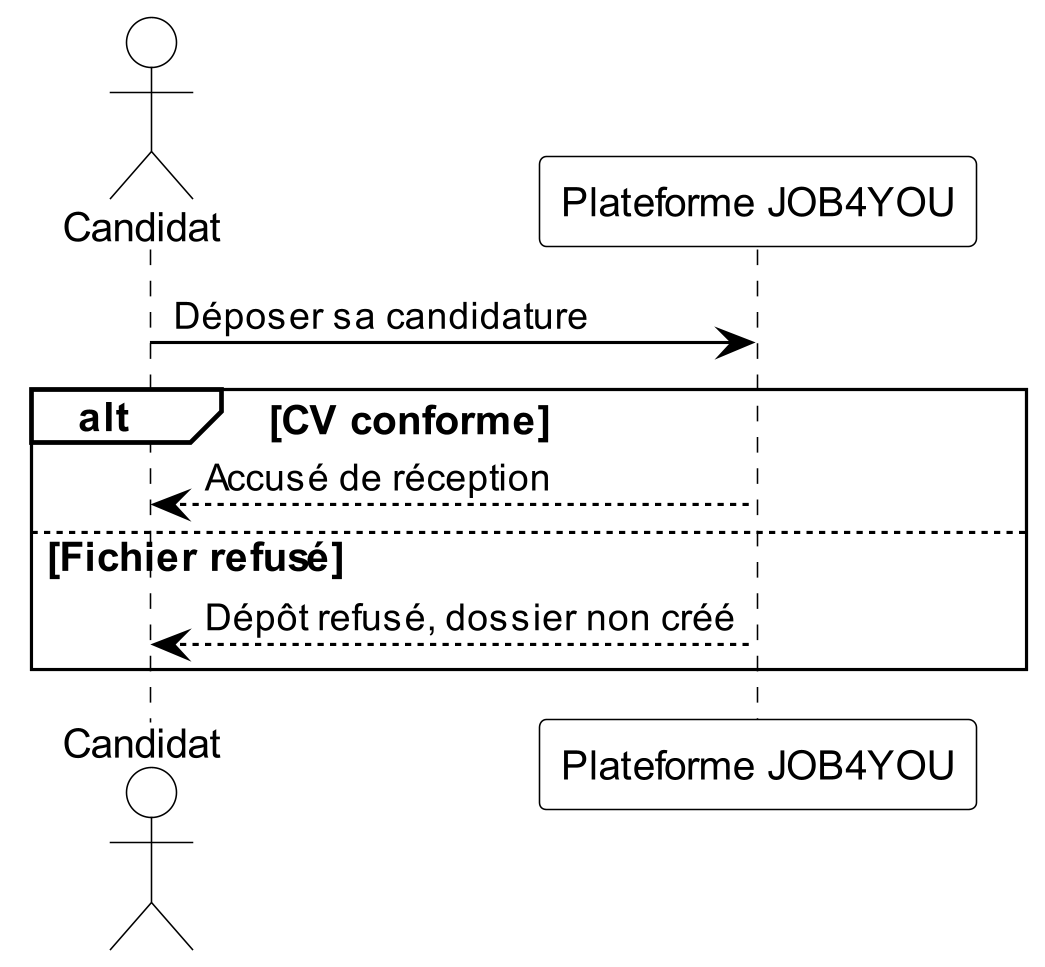
\includegraphics[width=240pt]{fig2_6}
\caption{Diagramme de séquence système — Dépôt d’une candidature (boîte noire)}
\label{fig_2_6}
\end{figure}

\section{Étude technique}
\label{sec_2_3}
Les choix techniques répondent aux besoins identifiés ; le tableau~\ref{tab_2_4} les résume.

% tableau 2.4
\setcounter{table}{2}
\begin{table}[!ht]
\centering
\caption{Technologies retenues et rôle dans JOB4YOU}
\label{tab_2_4}
\renewcommand{\arraystretch}{1.25}\footnotesize
\setlength{\tabcolsep}{4pt}%
\begin{tabular}{|P{0.19\textwidth}|P{0.29\textwidth}|P{0.40\textwidth}|}
\hline
\textbf{Technologie} & \textbf{Rôle dans JOB4YOU} & \textbf{Ce qui a décidé du choix} \\
\hline
\logo{spring} Spring Boot \cite{ref04,ref05} & Back-end et API REST & Spring Security et Spring Data JPA couvrent l’authentification et la persistance. \\
\hline
\logo{angular} Angular \cite{ref06,ref07} & Front-end de l’application & Composants, services et gardes de route conviennent à une interface à plusieurs rôles. \\
\hline
\logo{postgres} PostgreSQL \cite{ref08} & Offres, candidatures, entretiens & Transactions et clés étrangères sur des données fortement liées. \\
\hline
\logo{n8n} n8n \cite{ref09} & Notifications et planification & Workflows modifiables sans redéployer le back-end, services externes isolés. \\
\hline
\end{tabular}
\end{table}

\subsection{Architecture physique cible}
\label{sec_2_3_1}
La plateforme cible une architecture distribuée par couches : un front-end Angular servi au navigateur, un back-end Spring Boot exposant des API REST sécurisées, une base PostgreSQL (SGBD) et une couche d’automatisation n8n.

n8n porte deux responsabilités : la planification des entretiens (Google Calendar \cite{ref10}) et la totalité des notifications. Le back-end lui délègue tous ses courriels, tous ses rappels et toute réinitialisation du mot de passe, qu’il remet à la Gmail API par HTTPS. JavaMailSender ne subsiste que comme repli. Le back-end appelle Cohere \cite{ref11} pour le scoring et OpenRouter \cite{ref12} pour l’assistant.

Cette organisation physique est détaillée au chapitre 3 (figures~\ref{fig_3_10} et \ref{fig_3_11}) ; le tableau~\ref{tab_2_3} précise le rôle de chaque agent.

% tableau 2.3
\setcounter{table}{3}
\begin{table}[!ht]
\centering
\caption{Rôle des agents d’automatisation n8n}
\label{tab_2_3}
\renewcommand{\arraystretch}{1.25}\footnotesize
\setlength{\tabcolsep}{4pt}%
\begin{tabular}{|P{0.166\textwidth}|P{0.236\textwidth}|P{0.545\textwidth}|}
\hline
\textbf{Agent} & \textbf{Déclencheur} & \textbf{Rôle et traitement} \\
\hline
Agent 1 — « CV Parser + Score IA + Email Candidat » (scoring IA) & Déclenchement à la création d’une candidature (statut « candidature déposée ») & Extrait le texte du CV puis rappelle le back-end pour le recalcul du score. C’est le back-end, via son client d’analyse, qui interroge le service Cohere, calcule le score et le persiste ; le statut bascule ensuite vers « CV validé » ou « écarté d’office » selon le seuil. \\
\hline
Agent 2 — « Planification entretien + Email participants » (Google Meet et convocations) & Webhook déclenché à la planification d’un entretien & Crée réellement l’événement Google Calendar, génère le lien Google Meet correspondant, ajoute les participants et envoie la convocation au candidat comme la confirmation à l’intervieweur. \\
\hline
Agent 3 — « RH vers Manager (dossier validé) » (notification du manager désigné) & Déclenchements à l’entrée en évaluation technique (« test technique »), au rejet automatique et au retrait d’une candidature & Notifie le manager désigné par le RH, résolu et gelé sur le dossier par le back-end, sans dupliquer l’e-mail candidat ; les e-mails de décision — avis transmis au RH, convocation ou refus final adressé au candidat — sont émis par le back-end. \\
\hline
\end{tabular}
\end{table}
\subsection{Côté client — Angular}
\label{sec_2_3_2}
J’ai développé le front-end en SPA Angular, avec des composants autonomes. Il couvre les pages publiques (accueil, offres, candidature en ligne), les pages d’administration (candidats, entretiens, feedbacks, offres, utilisateurs, Kanban, tableau de bord) et les services partagés qui parlent à l’API REST du back-end. Bootstrap assure la mise en forme.

\subsection{Côté serveur — Spring Boot}
\label{sec_2_3_3}
Le back-end est écrit en Java sous Spring Boot 3, en couches : contrôleurs REST, services métier, repositories Spring Data JPA, entités JPA mappées sur PostgreSQL par Hibernate. Chacun reste à sa place, ce qui allège les évolutions.

\subsection{La sécurité — Spring Security et JWT}
\label{sec_2_3_4}
L’accès repose sur Spring Security \cite{ref13} et un jeton JWT : à la connexion, le serveur signe un jeton portant identité et rôles, qui revient dans l’en-tête de chaque requête, sans état de session. Chaque point d’entrée est filtré par l’annotation @PreAuthorize, qui réserve la ressource aux rôles autorisés.

\section{Conclusion}
\label{sec_2_4}
Acteurs, besoins et architecture étant désormais identifiés, reste à traduire tout cela en un modèle concret capable de guider le développement : c’est l’objet du chapitre suivant.

        % ======== fin chap_02 ========
        \clearpage
        
        \jobFixLists{chap03}
        % ======== chap_03 ========
\chapter{Conception}

Passer d’une liste de besoins à un système cohérent implique des choix : comment organiser le code, comment modéliser les données, comment éviter qu’un candidat se retrouve dans un état incohérent. Ce chapitre documente les principales décisions de conception derrière JOB4YOU — paquetages, diagramme de classes, scénarios d’interaction et machine à états du cycle de vie d’une candidature.

\section{Introduction}
\label{sec_3_1}
Chaque modèle présenté ici sert directement l’implémentation décrite au chapitre 4 : chaque diagramme correspond à une décision de conception effectivement prise pendant le développement.

\section{Diagramme des paquetages}
\label{sec_3_2}
La figure~\ref{fig_3_1} montre les paquetages du back-end : configuration, sécurité, contrôleurs, services, repositories et entités. L’organisation du front-end et les interactions avec les services externes sont détaillées aux sections~\ref{sec_3_8} et \ref{sec_3_9}.

% figure 3.1
\setcounter{figure}{0}
% le portrait a ete garde ici : ratio 1,23, le vrai paysage ne l agrandissait que de
% 10 % (534 pt contre 484 de large) tout en coutant une page pleine et la coupure
% du texte. En portrait l image imprime 10,0 pt, au-dessus de la cible de 8 pt.
\begin{figure}[!ht]
\centering
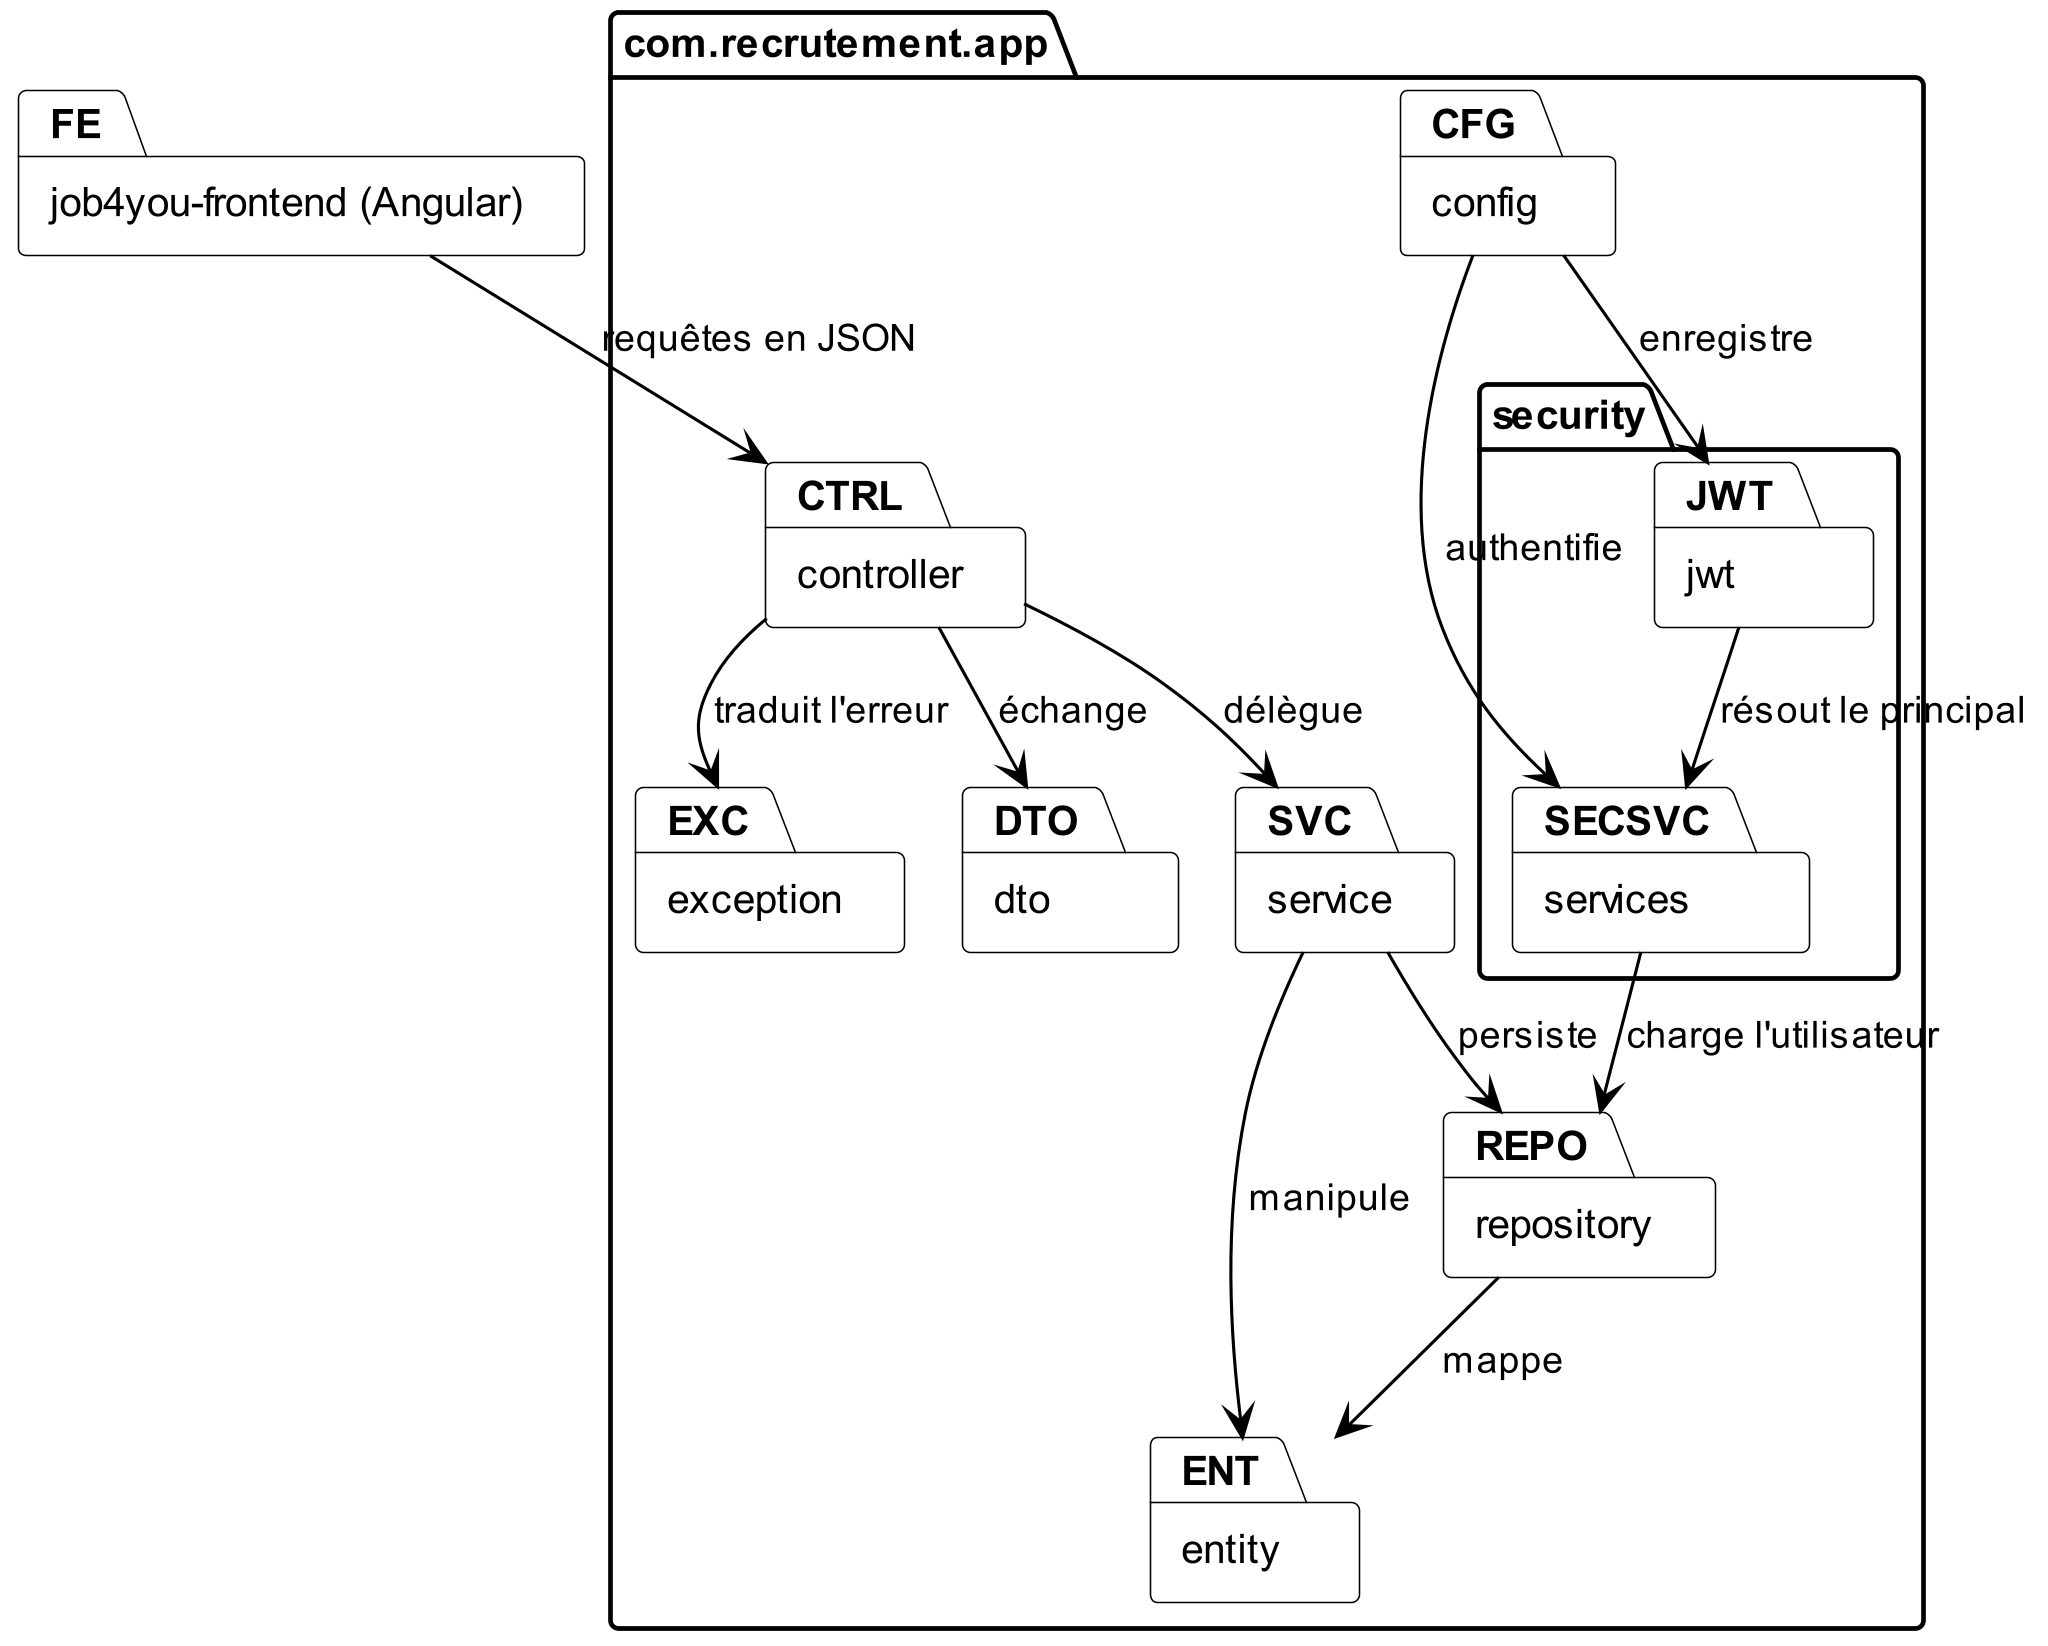
\includegraphics[width=\linewidth, height=0.94\textheight, keepaspectratio]{fig3_1}
\caption{Diagramme des paquetages}
\label{fig_3_1}
\end{figure}

Côté back-end, j’ai suivi un découpage classique en couches.
\begin{itemize}
\item \texttt{controller} : expose les API REST ;
\item \texttt{service} : porte la logique métier — règles de gestion, garde-fous, orchestration des appels vers n8n ;
\item \texttt{repository} : assure la persistance via Spring Data JPA ;
\item les entités JPA : modélisent le domaine.
\end{itemize}
Côté front-end, chaque page consomme des services Angular dédiés à une ressource métier, qui appellent le back-end en HTTP authentifié.

\section{Diagrammes de classes}
\label{sec_3_3}
Le modèle statique est présenté en trois volets, pour que chaque figure se lise sans zoom : cœur métier (figure~\ref{fig_3_2}), utilisateurs, rôles et audit (figure~\ref{fig_3_2a}), automatisation et tables d’accompagnement (figure~\ref{fig_3_2b}). La liste exhaustive des colonnes, types SQL et clés figure sur le schéma relationnel de la section~\ref{sec_3_7}.

Le trait suit la navigabilité réellement codée :

\begin{itemize}
\item association bidirectionnelle (un \texttt{@OneToMany} doublé de son \texttt{mappedBy}) : trait plein sans flèche ;
\item navigabilité unidirectionnelle (un \texttt{@ManyToOne} sans contre-référence) : flèche ouverte pointée vers la classe ciblée ;
\item lien logique porté par une simple colonne, sans clé étrangère en base : pointillés.
\end{itemize}

Les cardinalités sont rappelées à chaque extrémité. Seule la table d’association \texttt{user\_roles}, générée par le \texttt{@ManyToMany} de \texttt{User}, fait exception : ses deux traits pleins nomment les colonnes de la jointure sans rien dire de la navigabilité.

% figure 3_2
\setcounter{figure}{1}
\begin{figure}[!ht]
\centering
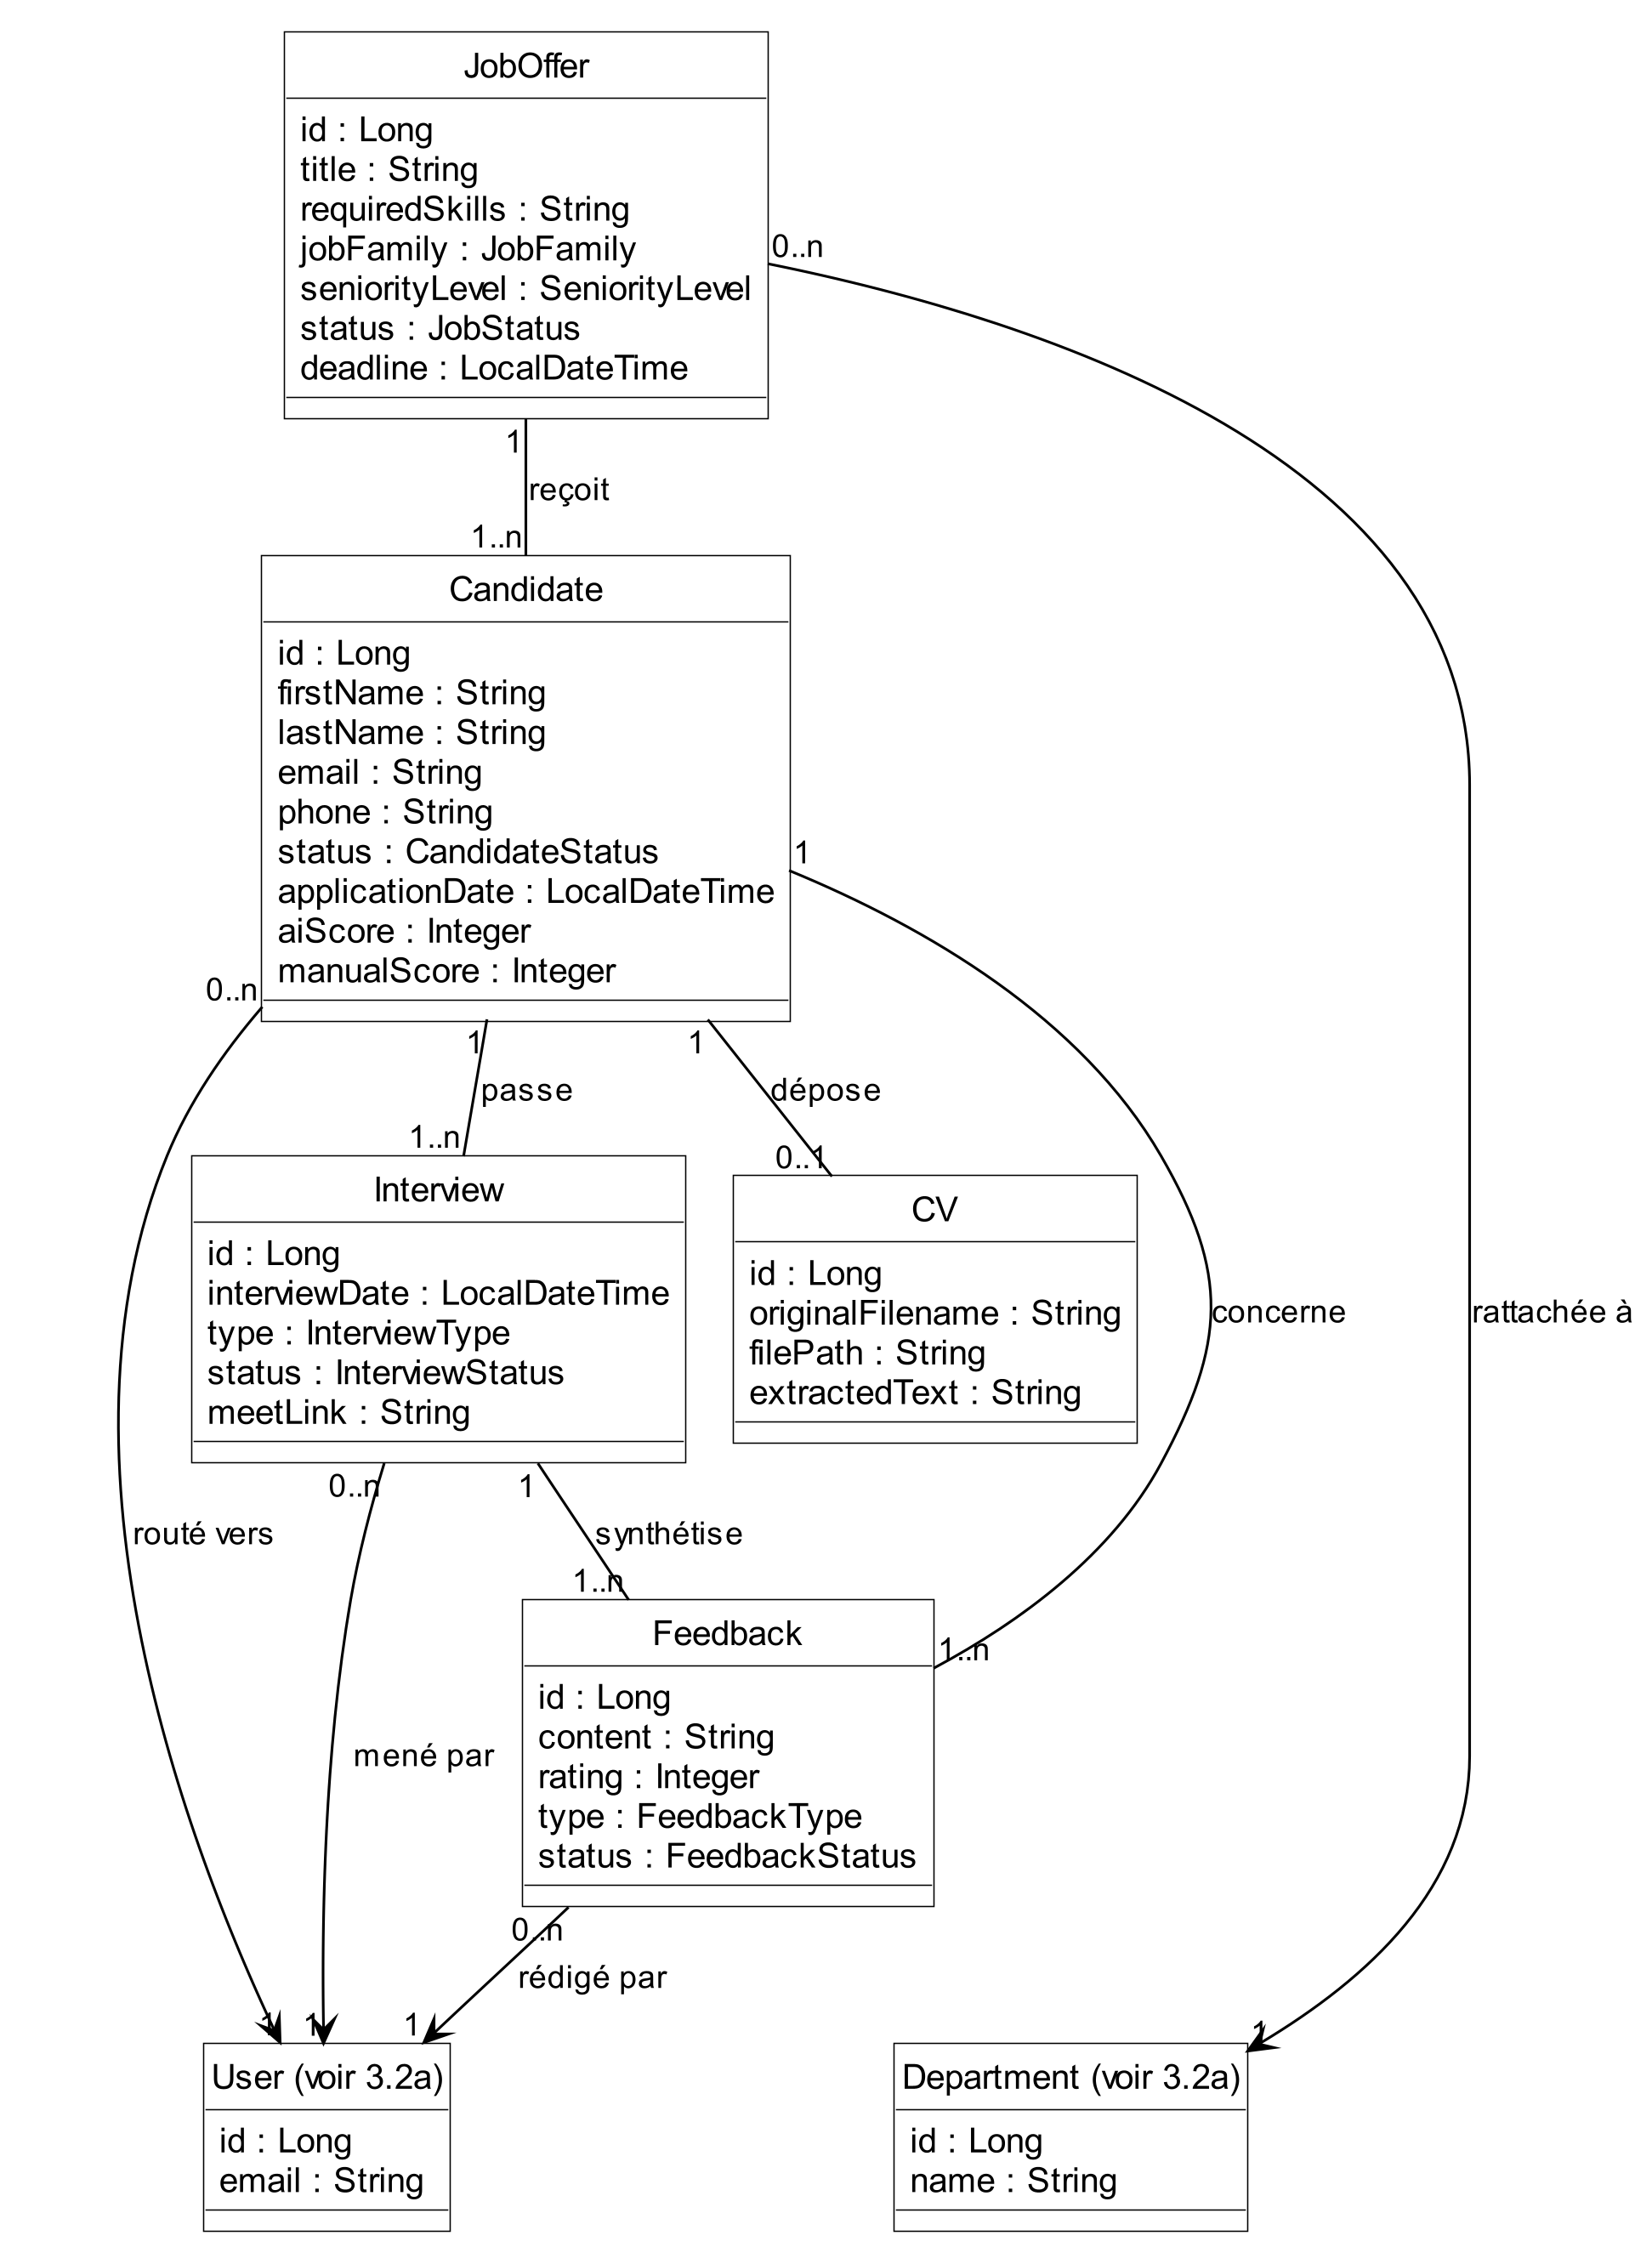
\includegraphics[width=\linewidth, height=0.94\textheight, keepaspectratio]{fig3_2}
\caption{Diagramme de classes — cœur métier du recrutement}
\label{fig_3_2}
\end{figure}

Ce premier volet concentre les cinq entités du parcours de recrutement, auxquelles s’ajoutent les rappels de \texttt{User} et de \texttt{Department}. Quatre relations unidirectionnelles aboutissent à ces deux classes : le dossier est routé vers un manager, l’entretien mené par un utilisateur, le retour rédigé par un utilisateur, l’offre rattachée à un département. Leur définition complète est donnée en figure~\ref{fig_3_2a}.

Un candidat dépose au plus un CV et peut passer plusieurs entretiens ; chaque entretien donne lieu à un retour, rattaché à la fois à l’entretien et au dossier ; une offre reçoit plusieurs candidatures.

Les deux scores conservés sur le dossier (\texttt{aiScore}, calculé par l’agent d’évaluation, et \texttt{manualScore}, saisi par le RH) traduisent une règle de conception : la décision reste traçable, chaque score portant son auteur et son horodatage.

% figure 3_2
\setcounter{figure}{1}
\begingroup\renewcommand{\thefigure}{3.2a}
\begin{figure}[!ht]
\centering
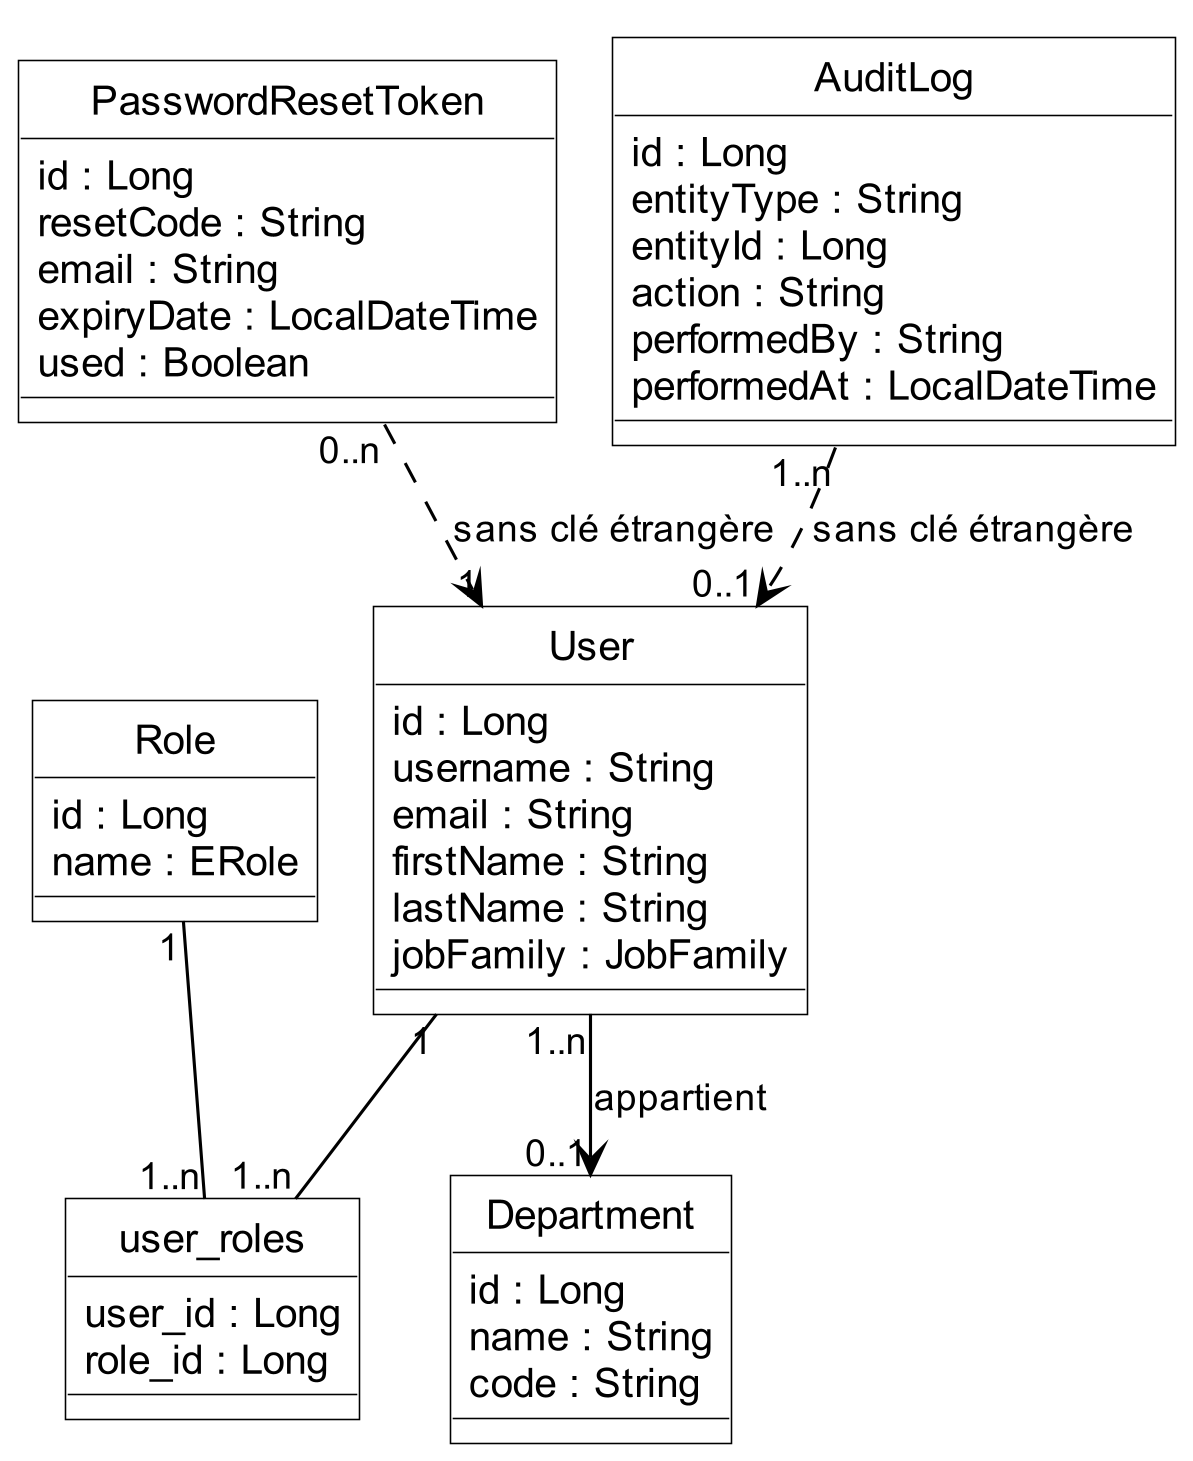
\includegraphics[width=370pt, keepaspectratio]{fig3_2a}
\caption{Diagramme de classes — utilisateurs, rôles et audit}
\label{fig_3_2a}
\end{figure}
\endgroup

La figure~\ref{fig_3_2a} isole la partie sécurité. La classe User centralise l’identité des comptes — RH, managers, administrateurs et candidats authentifiés, ces derniers avec le rôle ROLE\_USER ; les rôles multiples passent par la table d’association \texttt{user\_roles}, dessinée ici parce que JPA la génère sans entité correspondante. Le jeton de réinitialisation et la ligne d’audit s’y rattachent en pointillés : aucune clé étrangère derrière ces liens.

% figure 3_2
\setcounter{figure}{1}
\begingroup\renewcommand{\thefigure}{3.2b}
\begin{figure}[!ht]
\centering
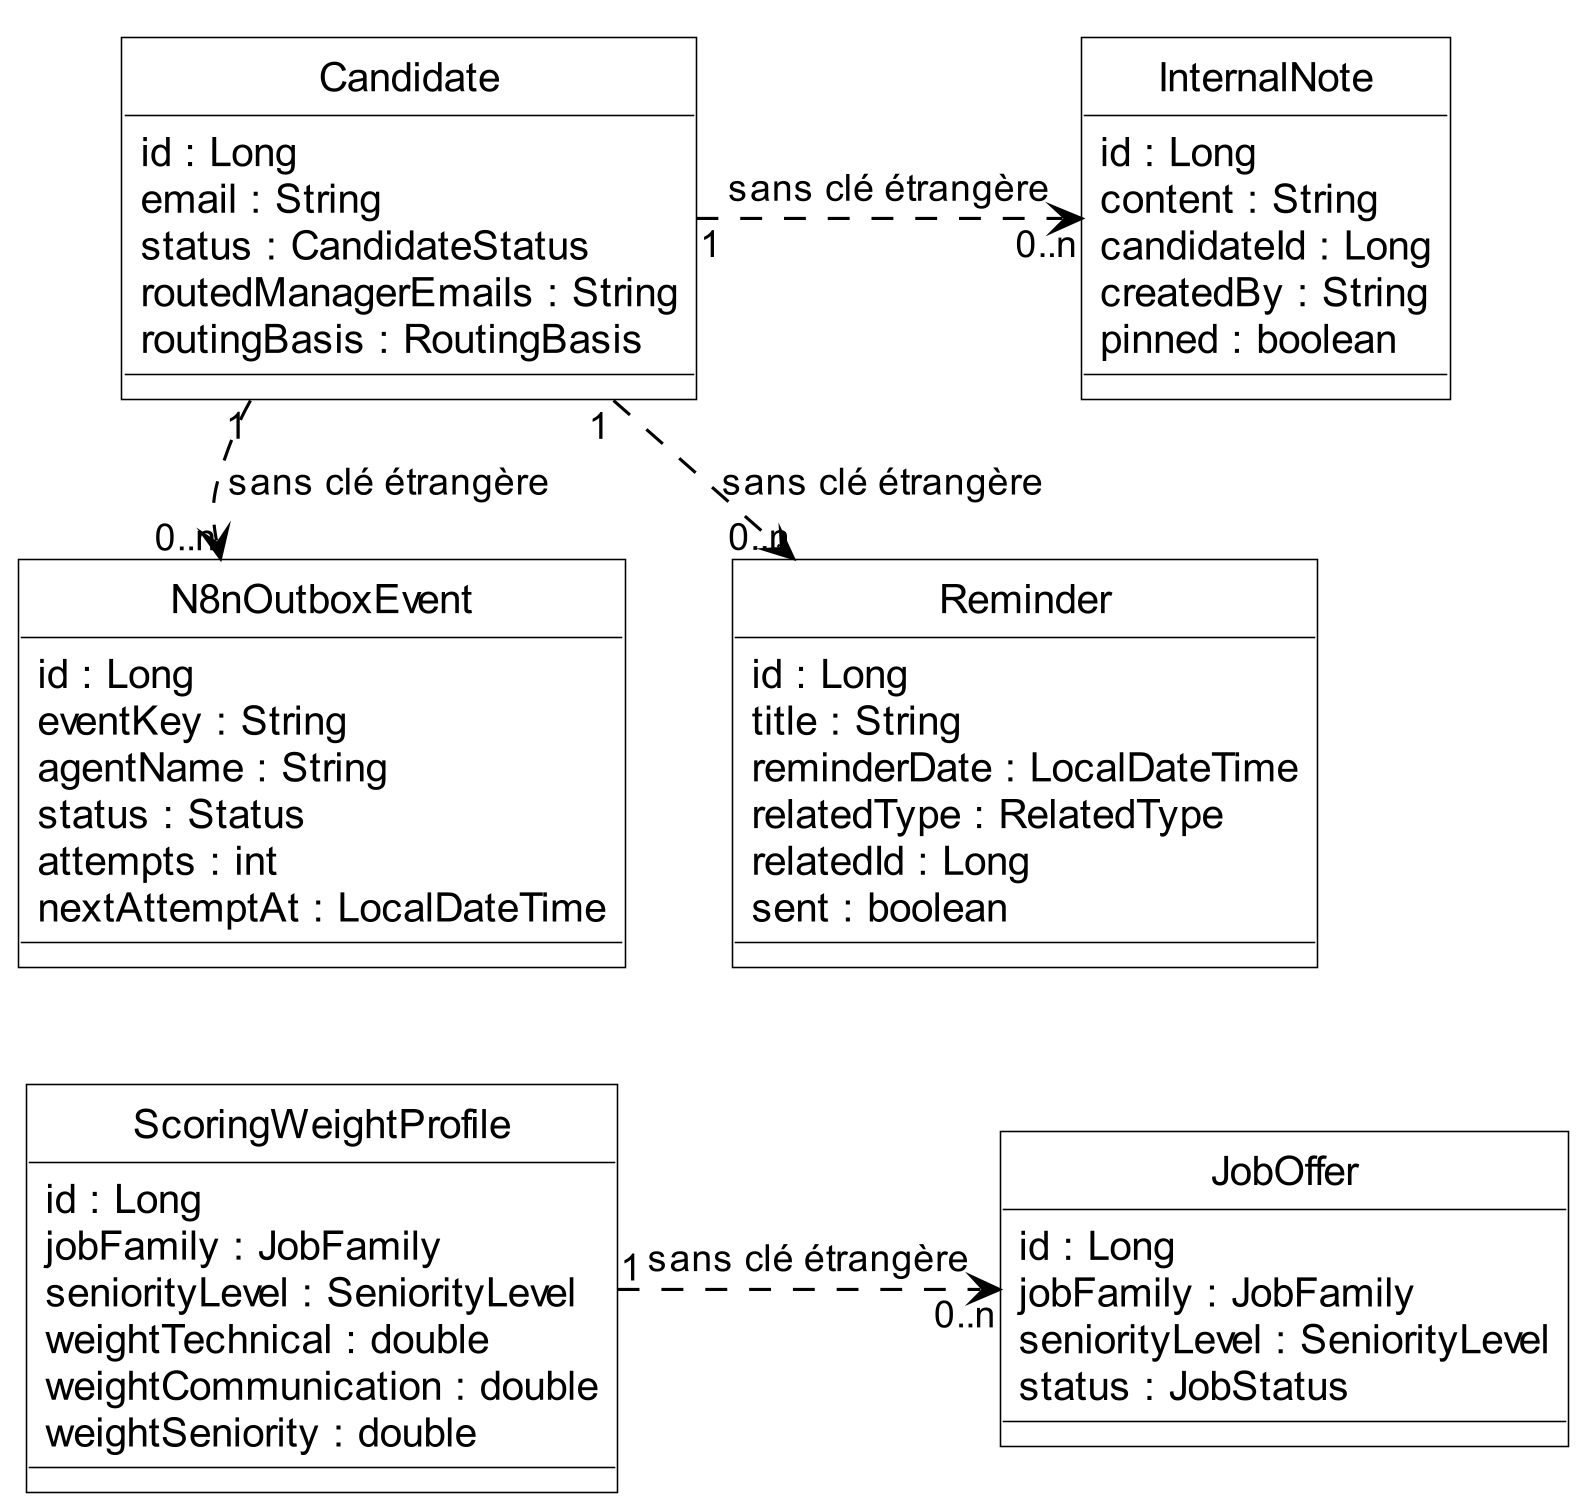
\includegraphics[width=\linewidth, height=0.94\textheight, keepaspectratio]{fig3_2b}
\caption{Diagramme de classes — automatisation et tables d’accompagnement}
\label{fig_3_2b}
\end{figure}
\endgroup

Le dernier volet réunit les entités qui prolongent le dossier sans toucher à son cycle de vie : file d’attente n8n, notes internes, rappels et profil de pondération. Deux liens se passent de clé étrangère : l’historique se retrouve par convention sur \texttt{event\_key}, et le profil de pondération s’applique par famille de métier et niveau d’ancienneté. Le calibrage du seuil y ajoute deux prolongements : la table \texttt{gold\_set\_cases}, qui garde le corpus annoté avec son origine, et trois colonnes portées par la candidature pour l’étiquette « Profil Gold » — statut, auteur et horodatage de la décision RH.

\section{Séquence technique — Soumission asynchrone et scoring IA}
\label{sec_3_4}
Lors de la soumission, l’application orchestre ses composants de manière asynchrone pour ne pas bloquer l’utilisateur (figure~\ref{fig_3_3}). Angular transmet la charge utile au back-end, qui persiste la candidature sous le statut « candidature déposée ». Une file interne déclenche l’extraction du texte, puis un rappel authentifié amène le back-end à solliciter le service Cohere et à enregistrer le score de pertinence.

% figure 3.3
\setcounter{figure}{2}
\begin{landscape}
\pagestyle{lscape}
\begin{figure}[p]
\centering
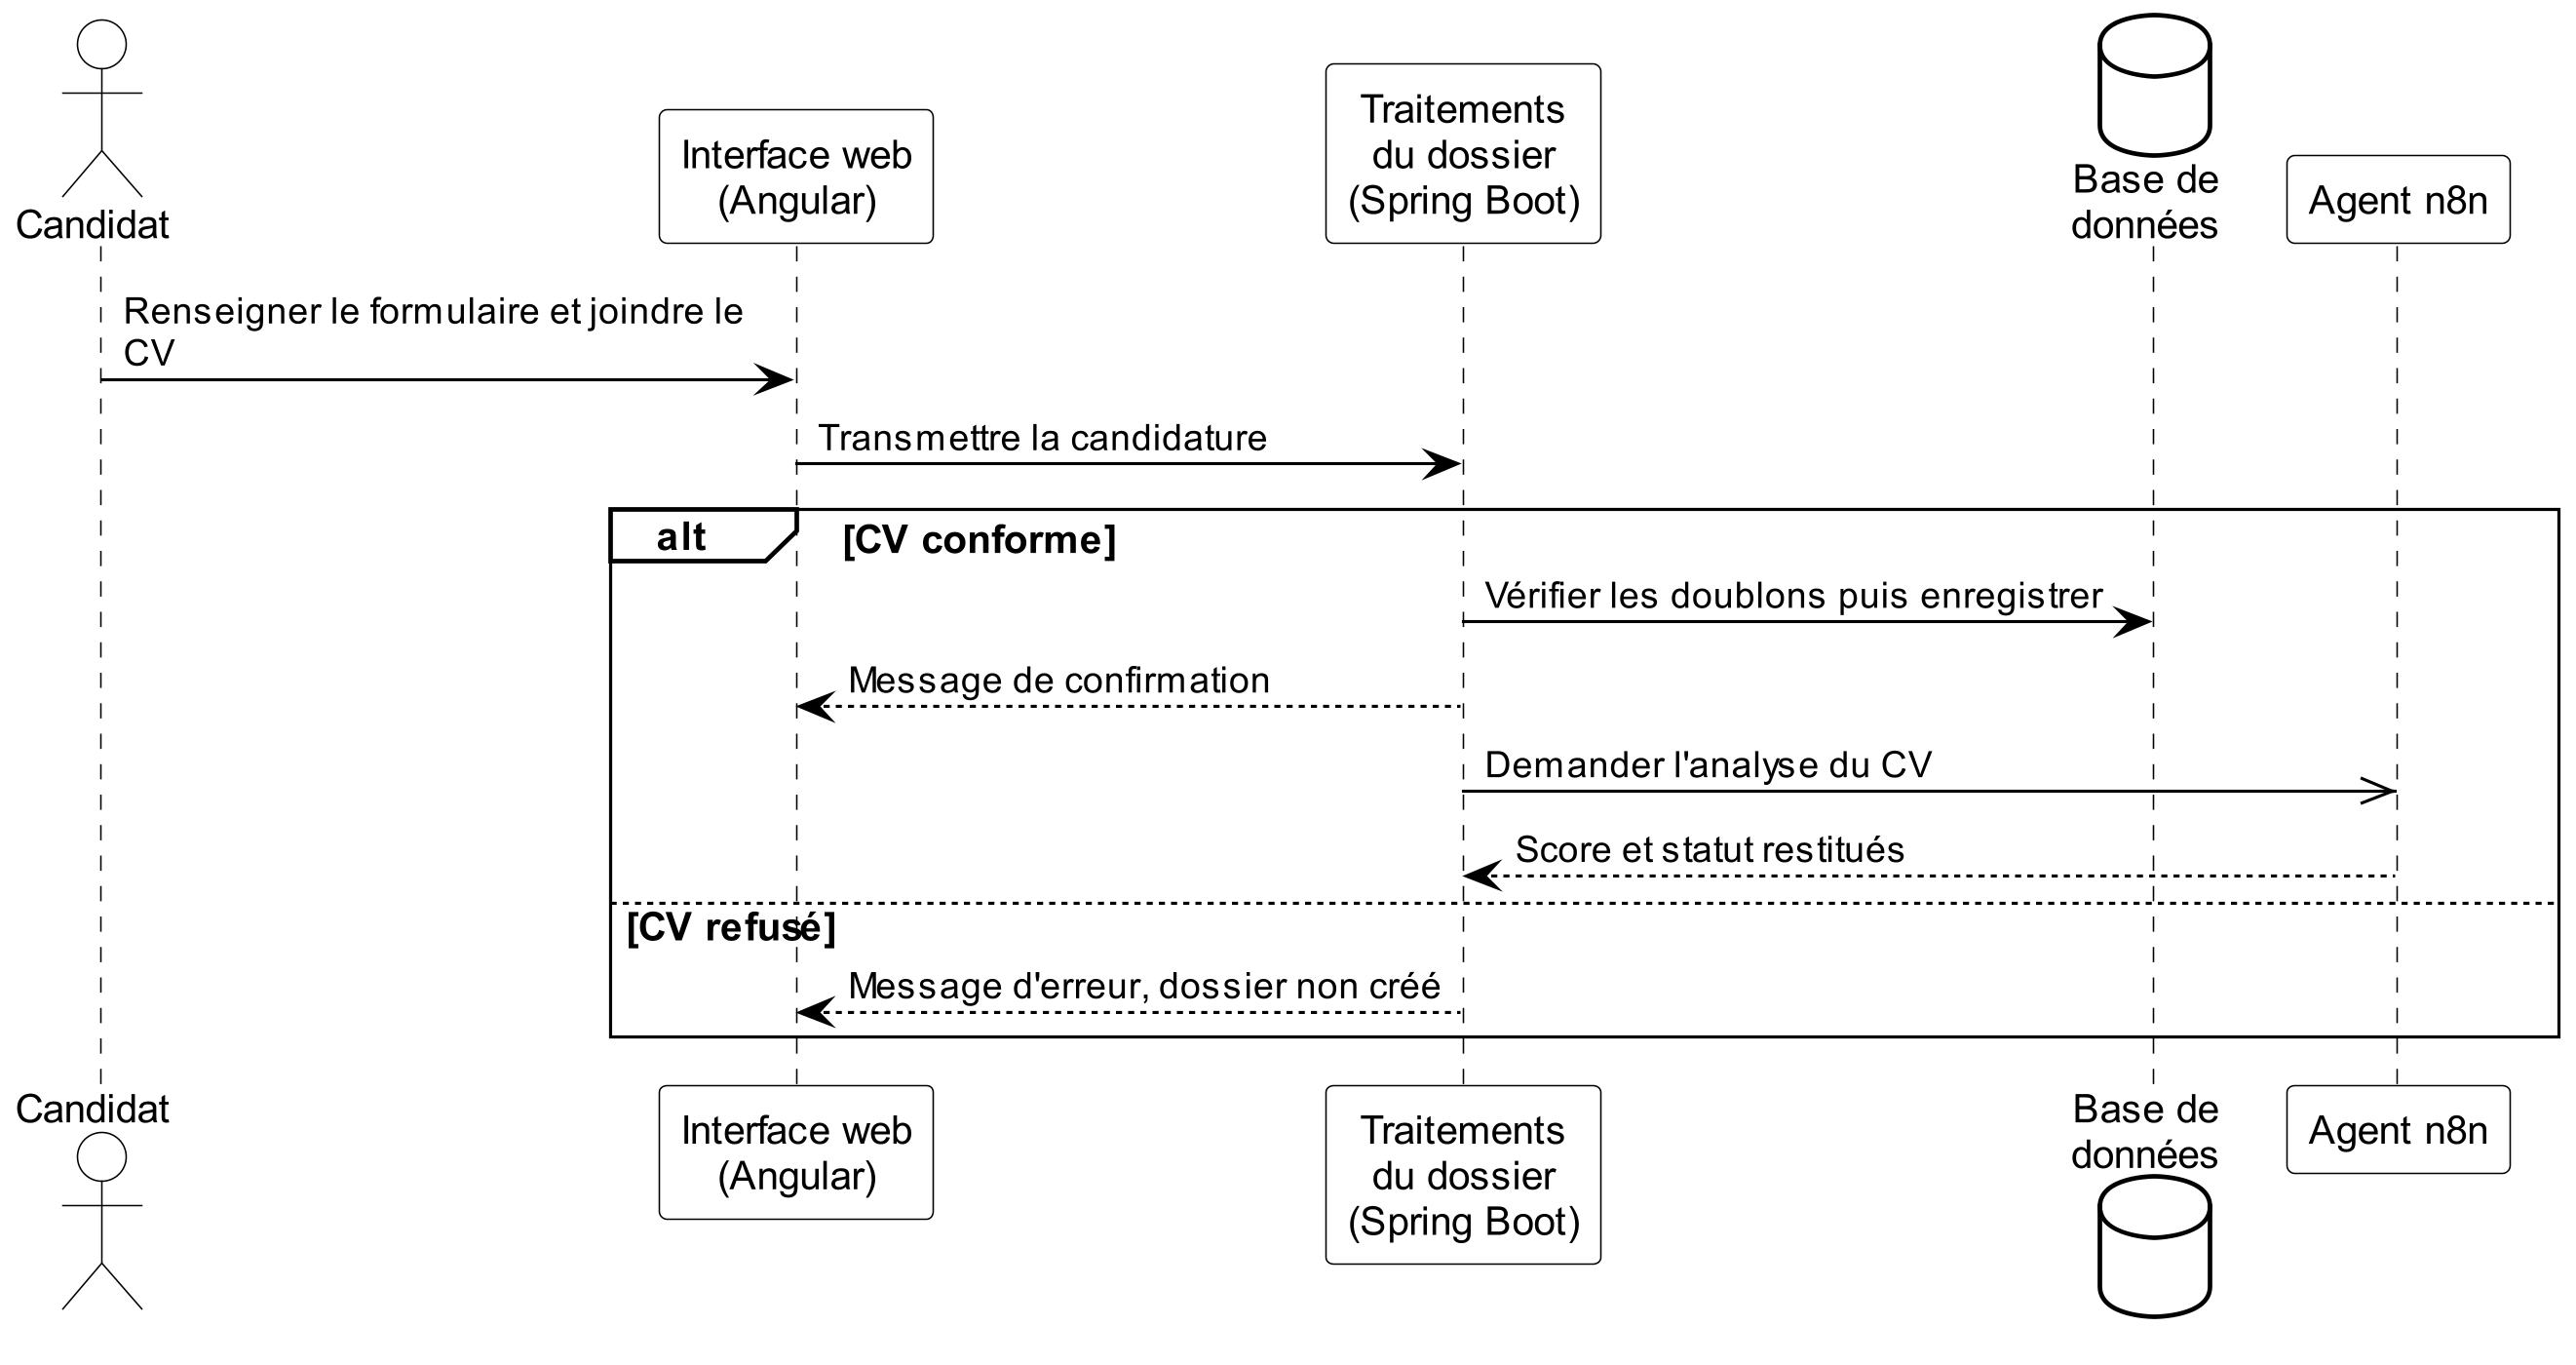
\includegraphics[width=0.98\linewidth, height=0.92\textheight, keepaspectratio]{fig3_3}
\caption{Diagramme de séquence technique — Soumission asynchrone et scoring IA}
\label{fig_3_3}
\end{figure}
\clearpage
\end{landscape}

\section{Diagrammes de séquence objet}
\label{sec_3_5}
Les figures de cette section détaillent, au niveau objet, quatre étapes clés du processus de recrutement : la planification d’un entretien, la décision finale, l’analyse du CV et le routage des managers. Trois d’entre elles sont présentées en deux volets, des figures~\ref{fig_3_4a} à \ref{fig_3_7b}, pour rester lisibles à l’impression. Chaque figure reste volontairement synthétique : elle montre le déroulement nominal et un unique cas d’échec, le plus fréquent ; les variantes de refus sont décrites dans le texte qui la suit.

\subsection{Planifier un entretien}
\label{sec_3_5_1}
% figures 3.4a et 3.4b
\setcounter{figure}{3}
\begingroup\renewcommand{\thefigure}{3.4a}
\begin{figure}[!ht]
\centering
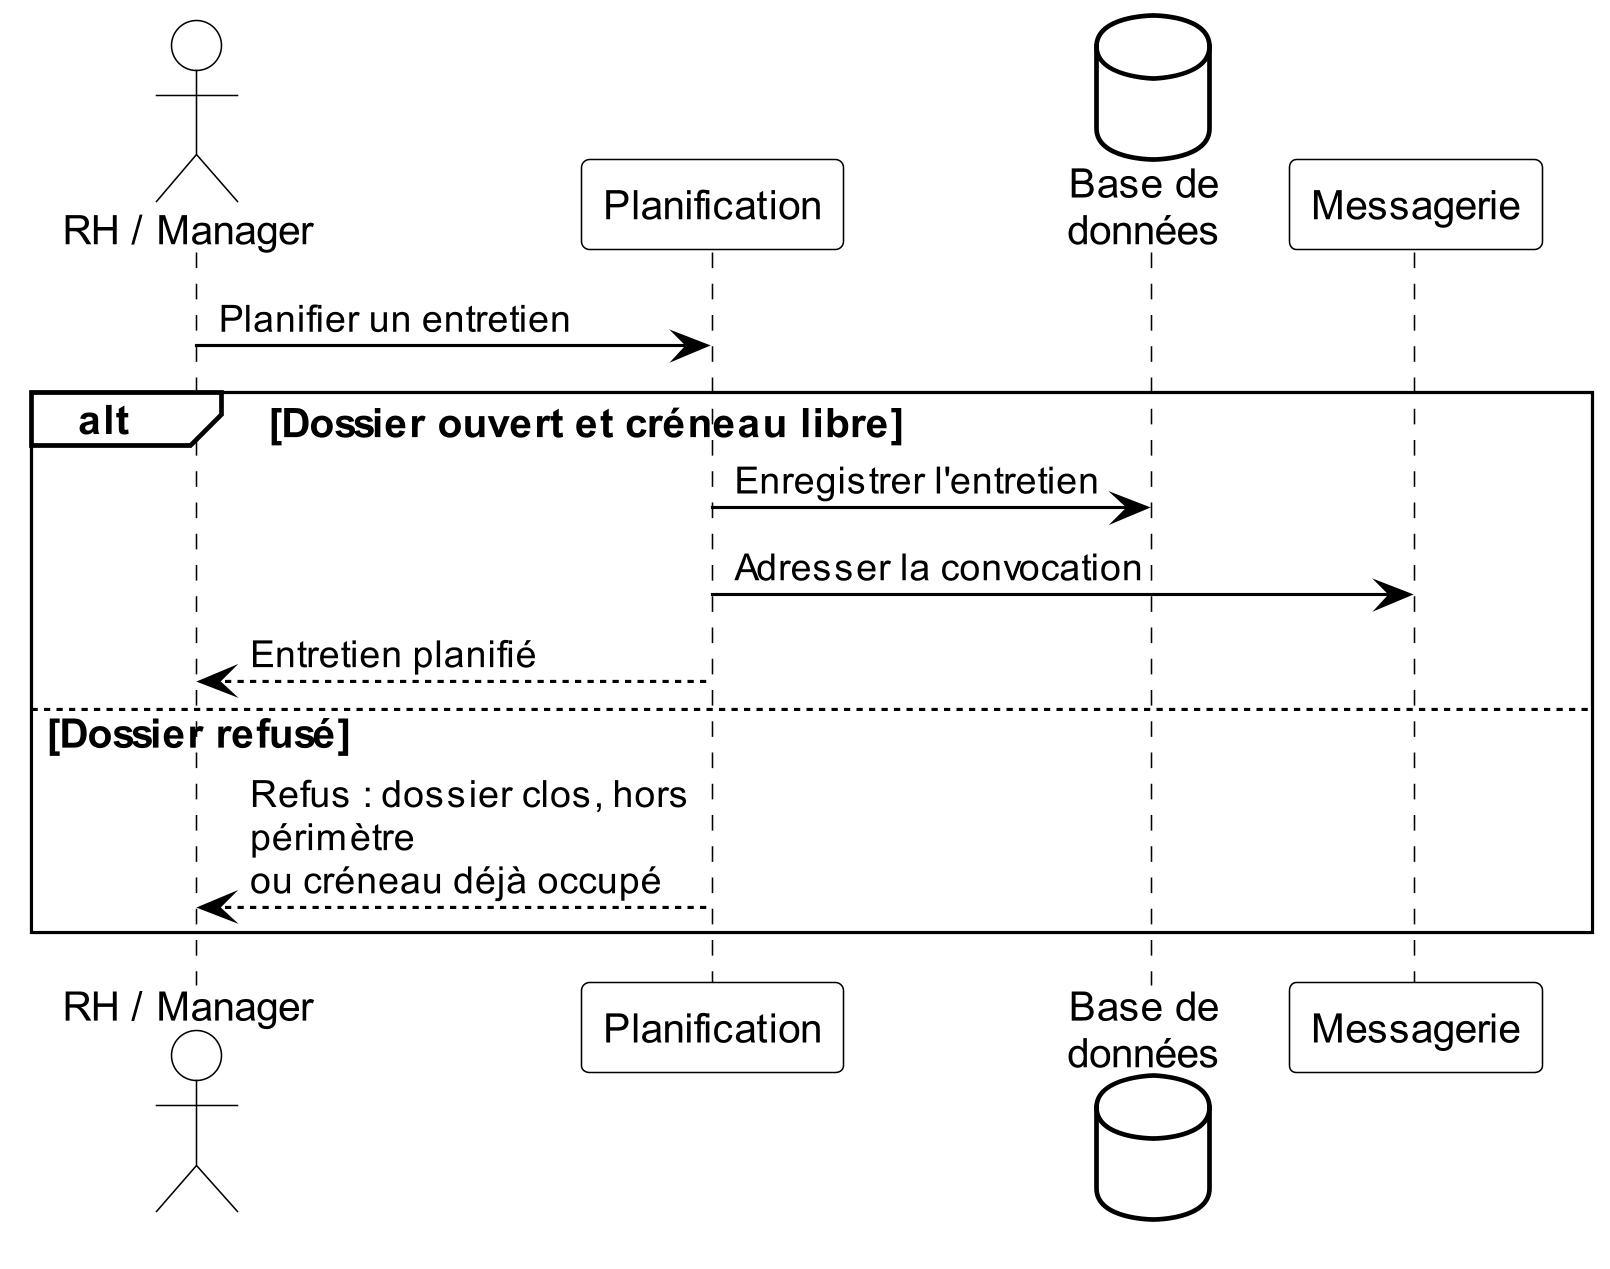
\includegraphics[width=\linewidth, height=0.94\textheight, keepaspectratio]{fig3_4a}
\caption{Diagramme de séquence objet — Planifier un entretien : demande et création de l’événement}
\label{fig_3_4a}
\end{figure}
\endgroup

\begingroup\renewcommand{\thefigure}{3.4b}
\begin{figure}[!ht]
\centering
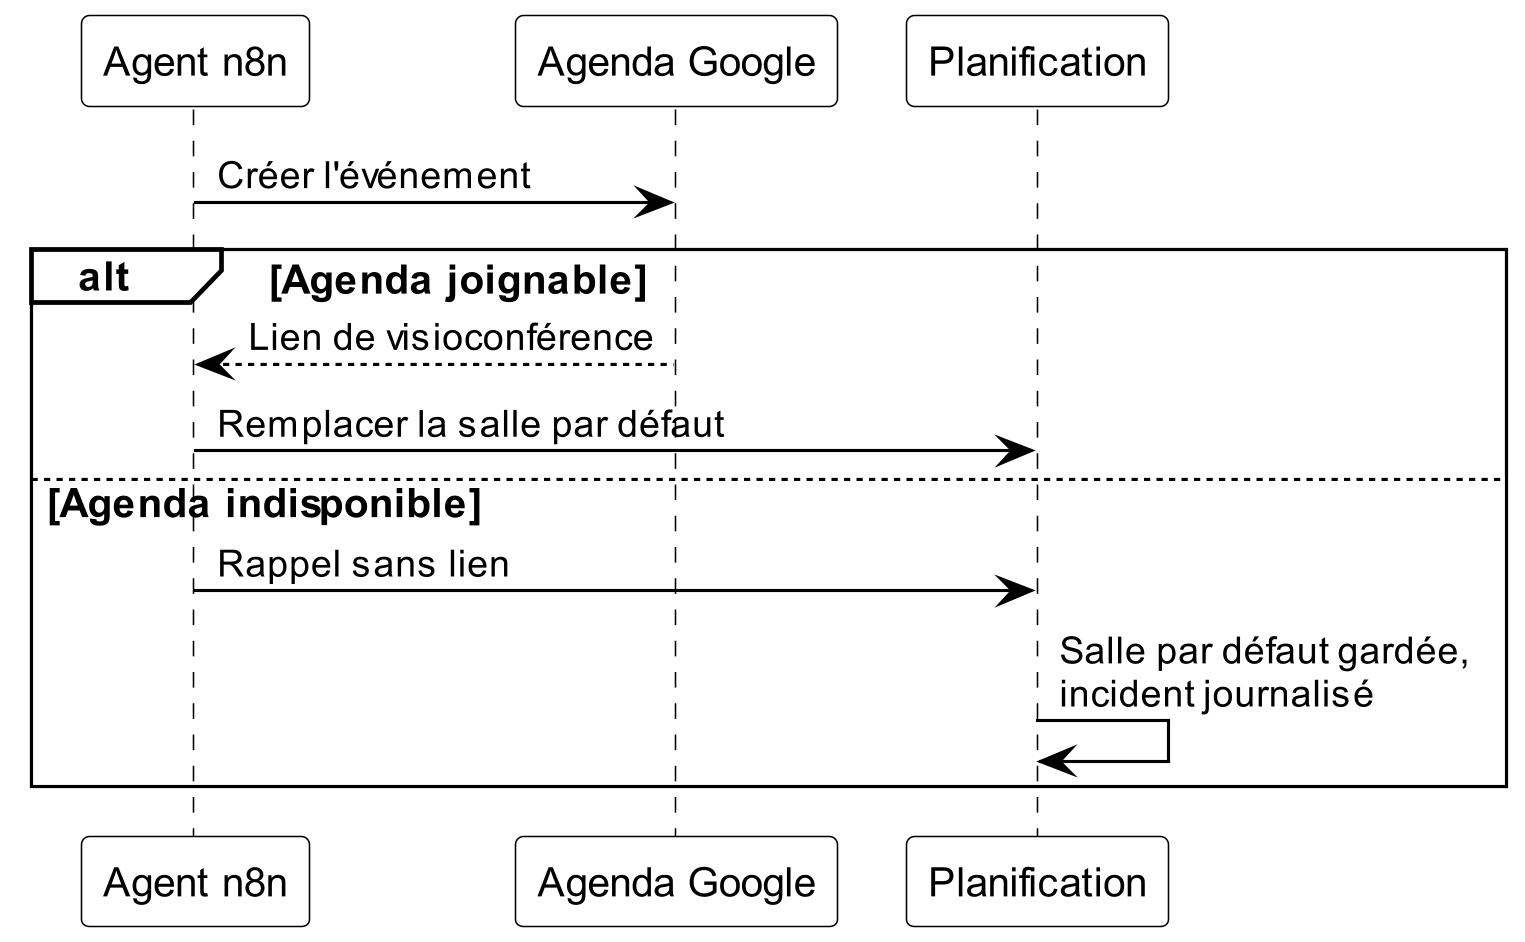
\includegraphics[width=\linewidth, height=0.94\textheight, keepaspectratio]{fig3_4b}
\caption{Diagramme de séquence objet — Planifier un entretien : lien de visioconférence et mise à jour du dossier}
\label{fig_3_4b}
\end{figure}
\endgroup

Le refus est groupé sur les figures~\ref{fig_3_4a} et~\ref{fig_3_4b}. Trois garde-fous le détaillent. La planification écarte un dossier clos ou un CV non examiné. Elle refuse tout créneau qui chevauche un entretien déjà réservé par le même intervieweur. Enfin, un manager ne planifie que dans son propre agenda, pour un dossier de son périmètre.

\subsection{Décision finale de recrutement}
\label{sec_3_5_2}
% figures 3.5a et 3.5b
\setcounter{figure}{4}
\begingroup\renewcommand{\thefigure}{3.5a}
\begin{figure}[!ht]
\centering
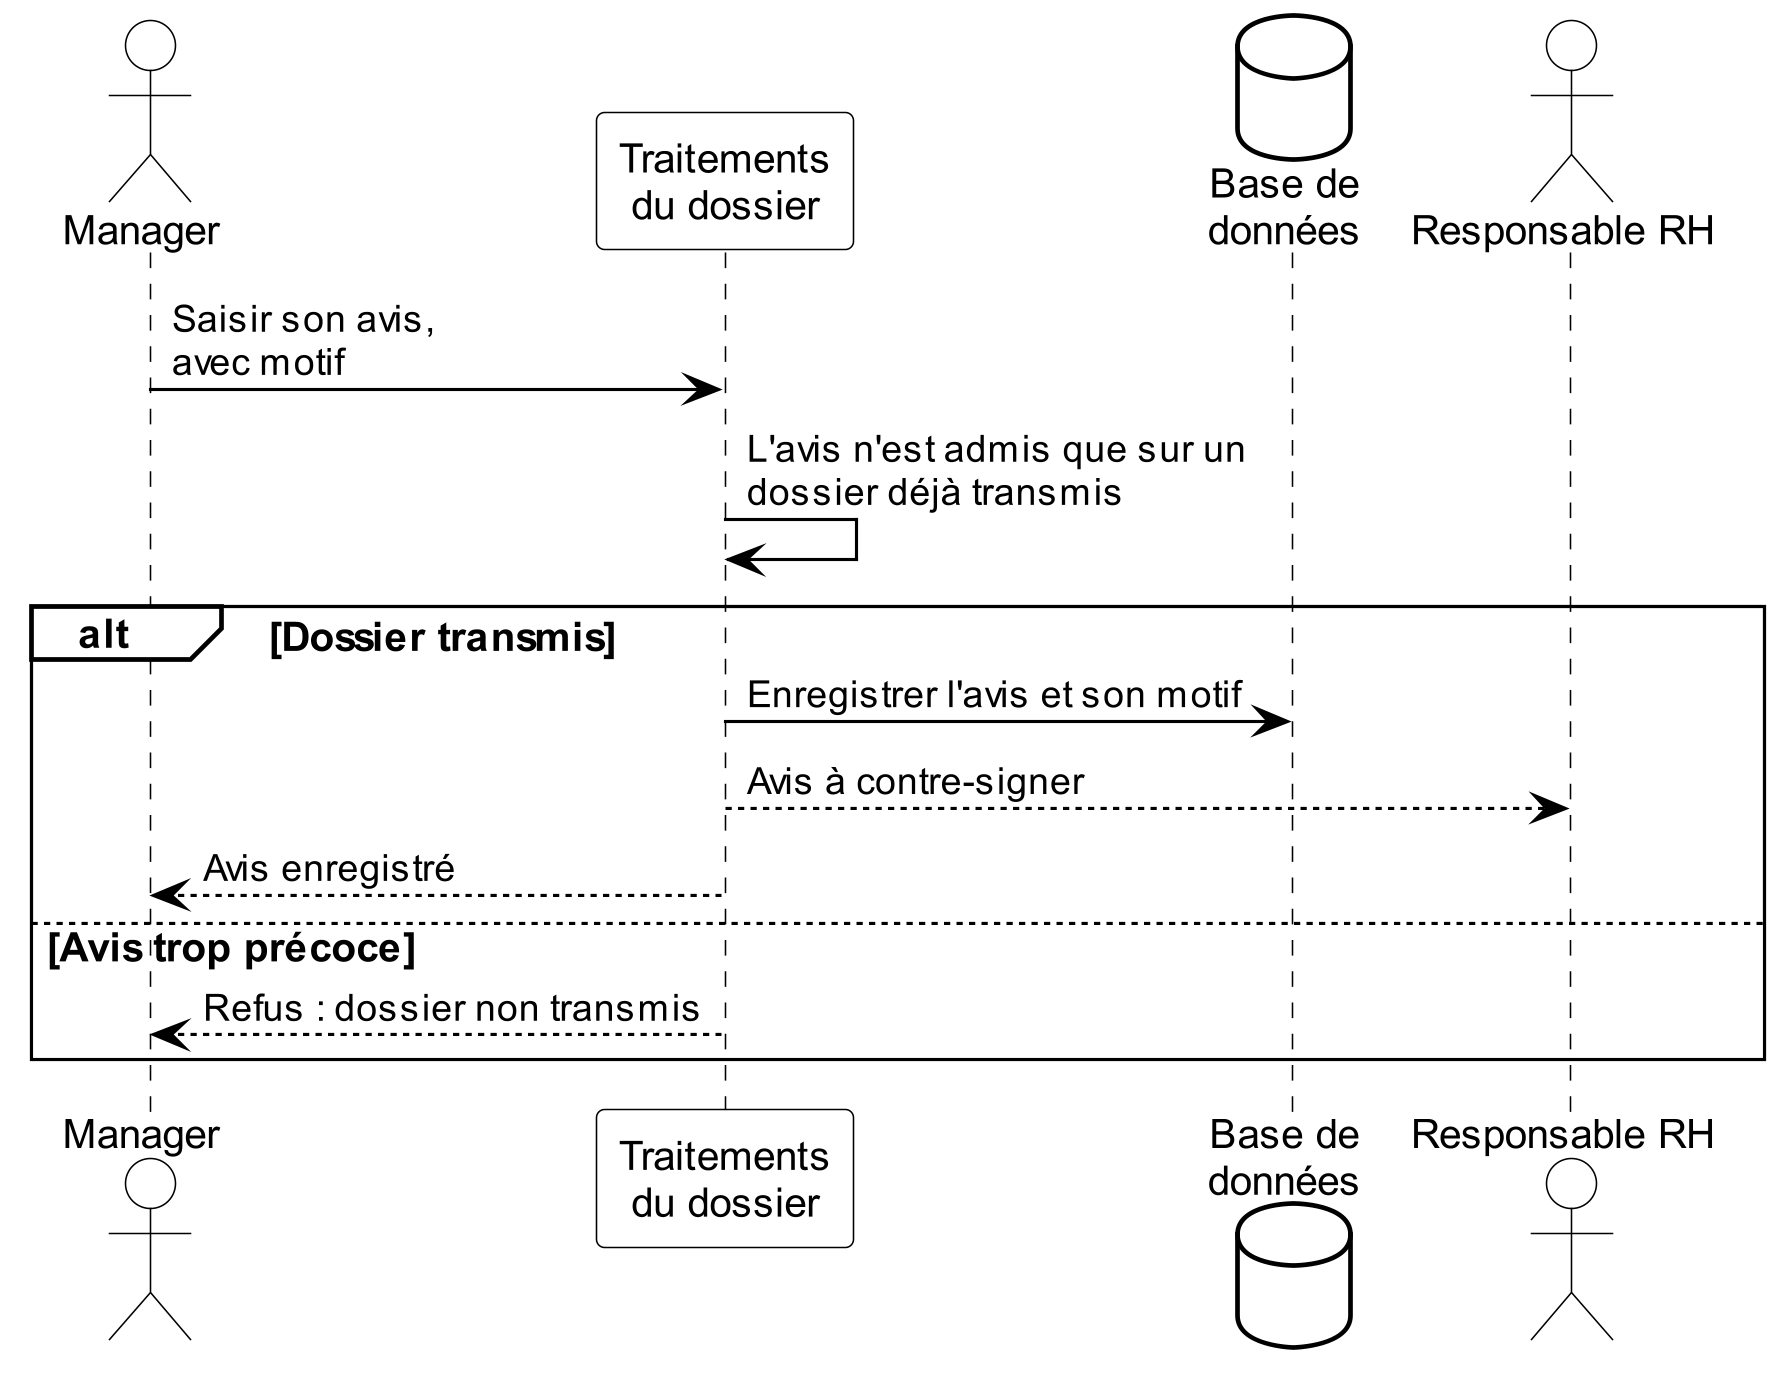
\includegraphics[width=\linewidth, height=0.94\textheight, keepaspectratio]{fig3_5a}
\caption{Diagramme de séquence objet — Décision finale : avis du manager}
\label{fig_3_5a}
\end{figure}
\endgroup

\begingroup\renewcommand{\thefigure}{3.5b}
\begin{figure}[!ht]
\centering
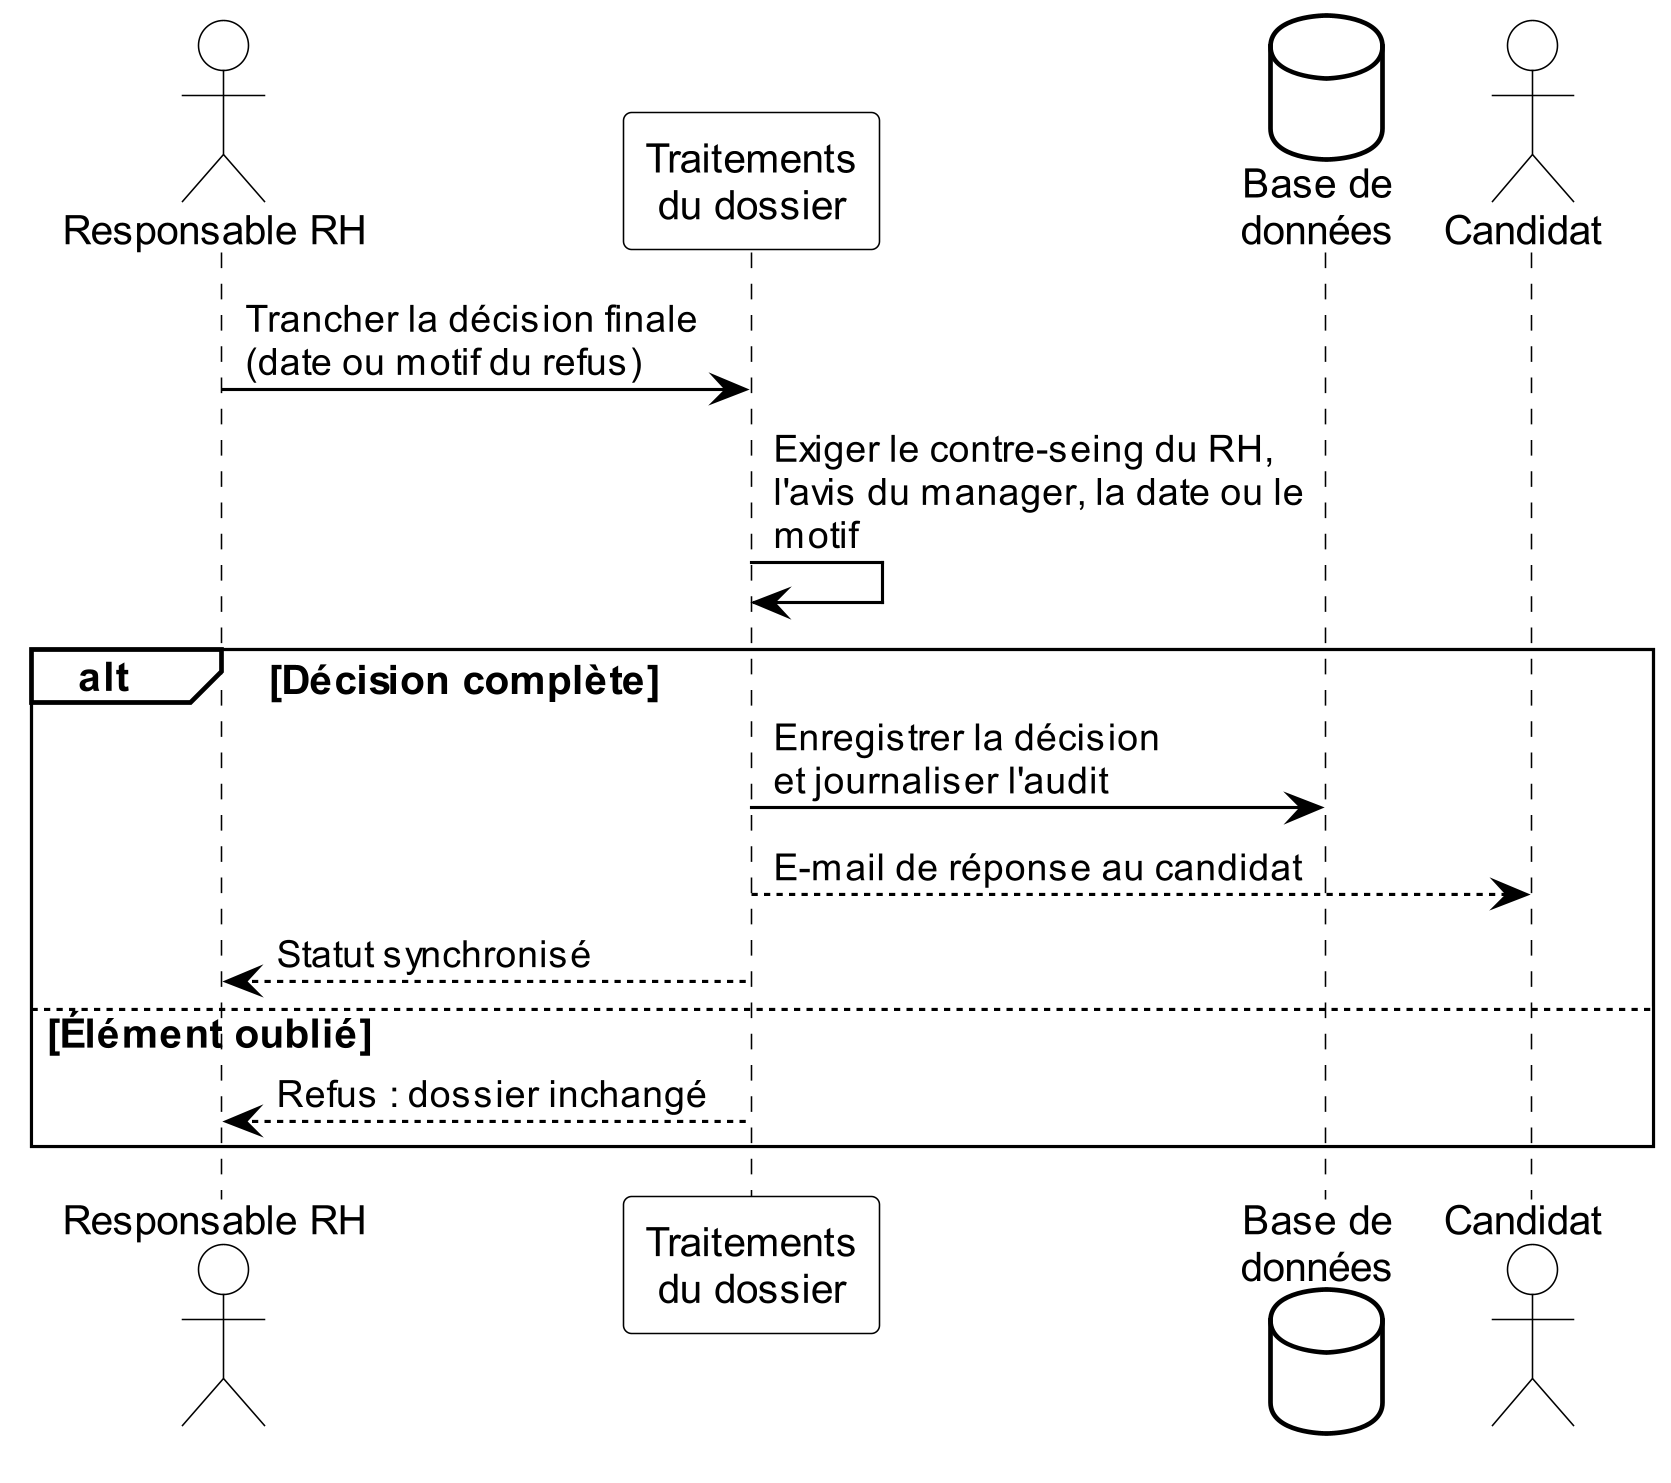
\includegraphics[width=\linewidth, height=0.94\textheight, keepaspectratio]{fig3_5b}
\caption{Diagramme de séquence objet — Décision finale : contreseing du responsable RH}
\label{fig_3_5b}
\end{figure}
\endgroup

Les figures~\ref{fig_3_5a} et~\ref{fig_3_5b} illustrent le garde-fou central : la décision est répartie sur deux niveaux. Le manager consulte le dossier et émet un avis (favorable ou refus motivé) uniquement sur un dossier transmis pour évaluation technique ; les étapes encore côté RH ne sont pas instruites par le manager.

L’avis est journalisé et notifie le responsable RH par e-mail et dans sa liste de candidats, sans aucun envoi au candidat. Le responsable RH, ou l’administrateur, contresigne ensuite : l’embauche exige la date de présentation des documents et déclenche la convocation ; le refus final exige un motif, enregistré sur le dossier et journalisé mais non communiqué au candidat, et déclenche l’e-mail de réponse.

Un compte purement manager ne peut pas franchir cette étape : la demande lui est refusée. Aucune candidature n’est donc retenue sans ce premier filtre humain (section~\ref{sec_4_5_8}), et aucun manager ne clôture seul le processus.

\subsection{Analyse du CV : extraction, score automatique et arbitrage}
\label{sec_3_5_3}
% figure 3.6 : remise en portrait (rapport 1,00), une page economilee
\setcounter{figure}{5}
\begin{figure}[!ht]
\centering
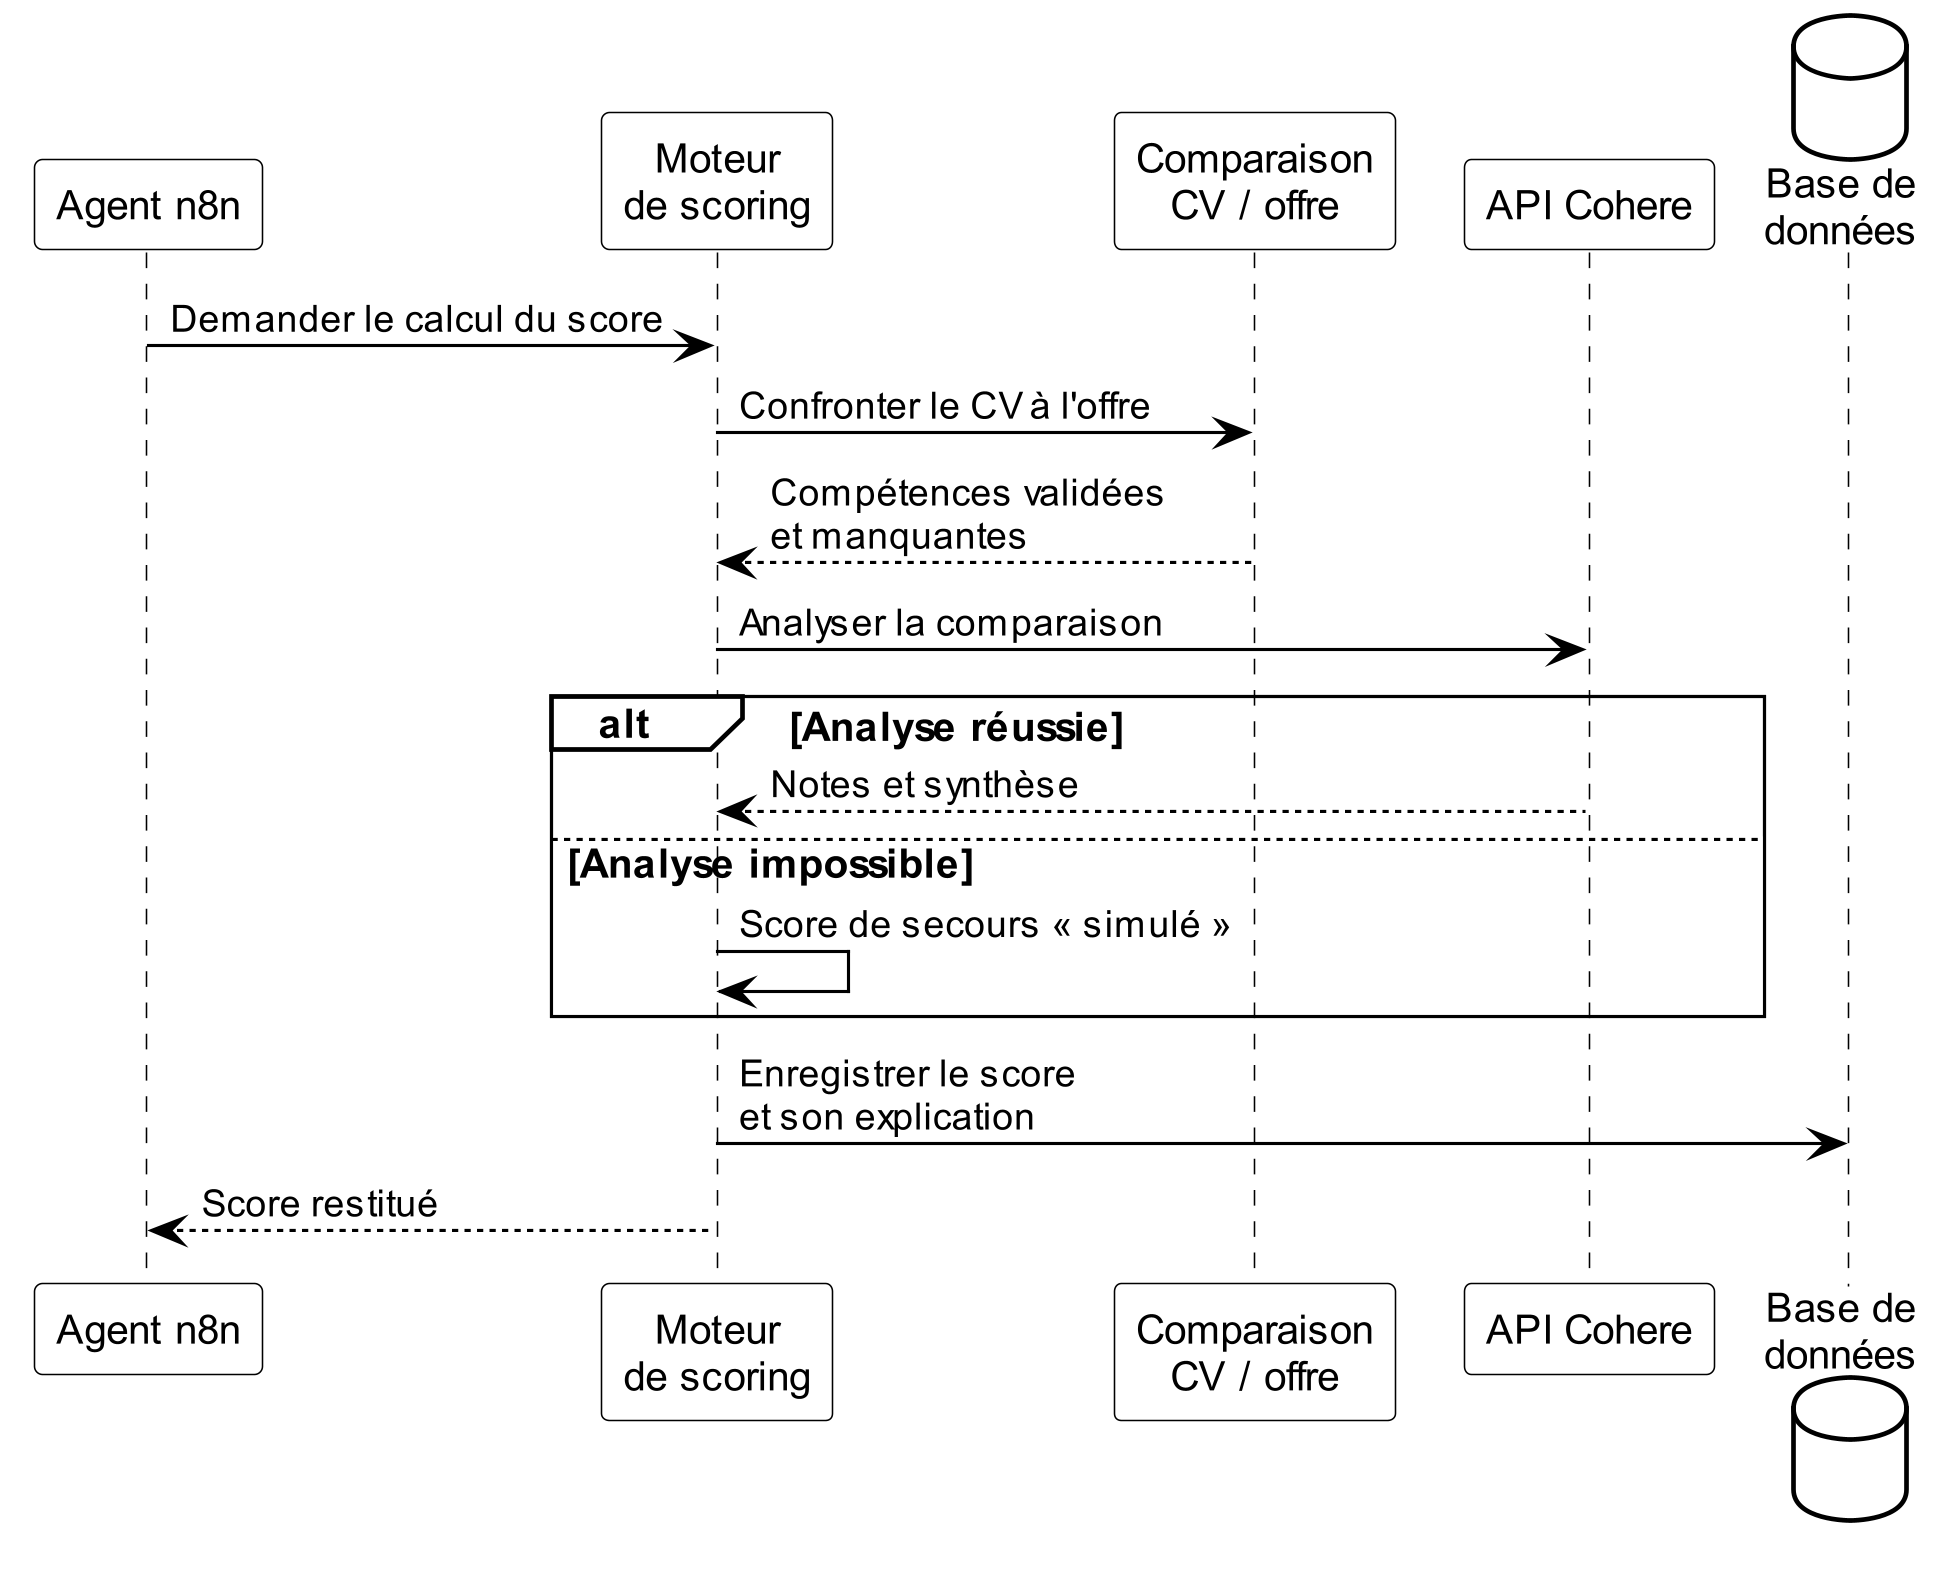
\includegraphics[width=\linewidth, height=0.94\textheight, keepaspectratio]{fig3_6}
\caption{Diagramme de séquence objet — Analyse du CV et calcul du score}
\label{fig_3_6}
\end{figure}

Le texte du CV est extrait par le back-end à la soumission, puis la candidature entre dans la file interne. L’agent de lecture est déclenché en arrière-plan et rappelle le back-end, qui interroge le service d’analyse, calcule le score et l’enregistre. Le statut bascule alors vers « CV validé » ou « écarté d’office » selon le seuil, sans intervention humaine.

La figure~\ref{fig_3_6} ne montre que le calcul du score et le cas où l’analyse aboutit difficilement. Deux étapes complémentaires prolongent ce parcours. Avant l’analyse, les compétences extraites sont harmonisées (k8s devient Kubernetes, postgres devient PostgreSQL) et les termes absents du dictionnaire d’alias sont conservés, afin qu’une compétence rare ne disparaisse pas du comparatif. Le dossier part ensuite en arbitrage humain plutôt qu’en décision automatique dans quatre cas :
\begin{itemize}
\item le texte extrait est absent ou compte moins de cinquante caractères ;
\item un écart de séniorité sévère plafonne le score ;
\item le score tombe dans la zone grise, à cinq points au-dessous ou au-dessus du seuil du profil ;
\item le service d’analyse est indisponible : le score est alors marqué à titre indicatif (section~\ref{sec_4_4_6}).
\end{itemize}

\subsection{Passage en évaluation technique — routage et notification des managers}
\label{sec_3_5_4}
% figures 3.7a et 3.7b : decoupage en deux volets, remise en portrait
\setcounter{figure}{6}
\begingroup\renewcommand{\thefigure}{3.7a}
\begin{figure}[!ht]
\centering
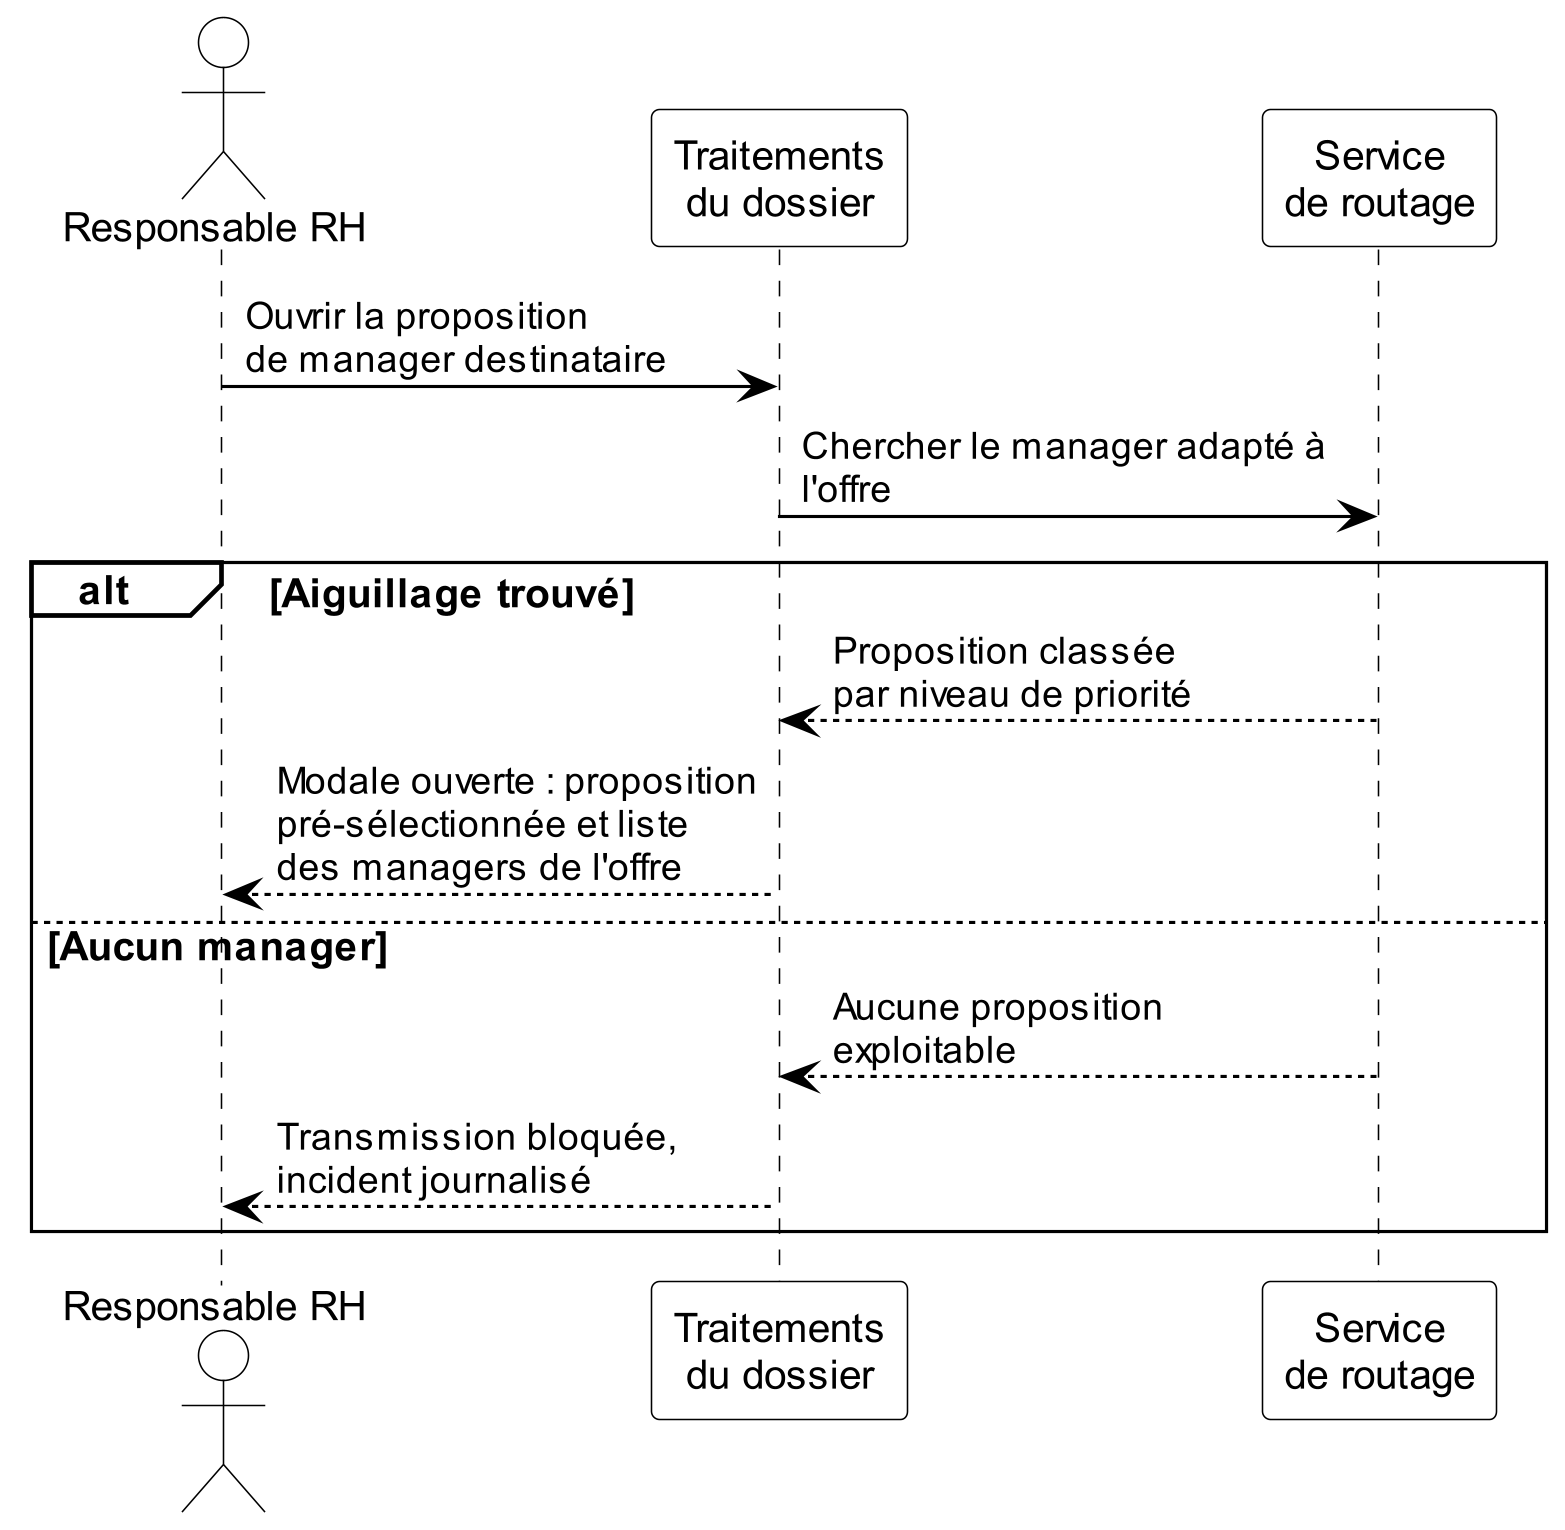
\includegraphics[width=460pt, keepaspectratio]{fig3_7a}
\caption{Diagramme de séquence objet — Routage des managers : désignation du destinataire}
\label{fig_3_7a}
\end{figure}
\endgroup

\begingroup\renewcommand{\thefigure}{3.7b}
\begin{figure}[!ht]
\centering
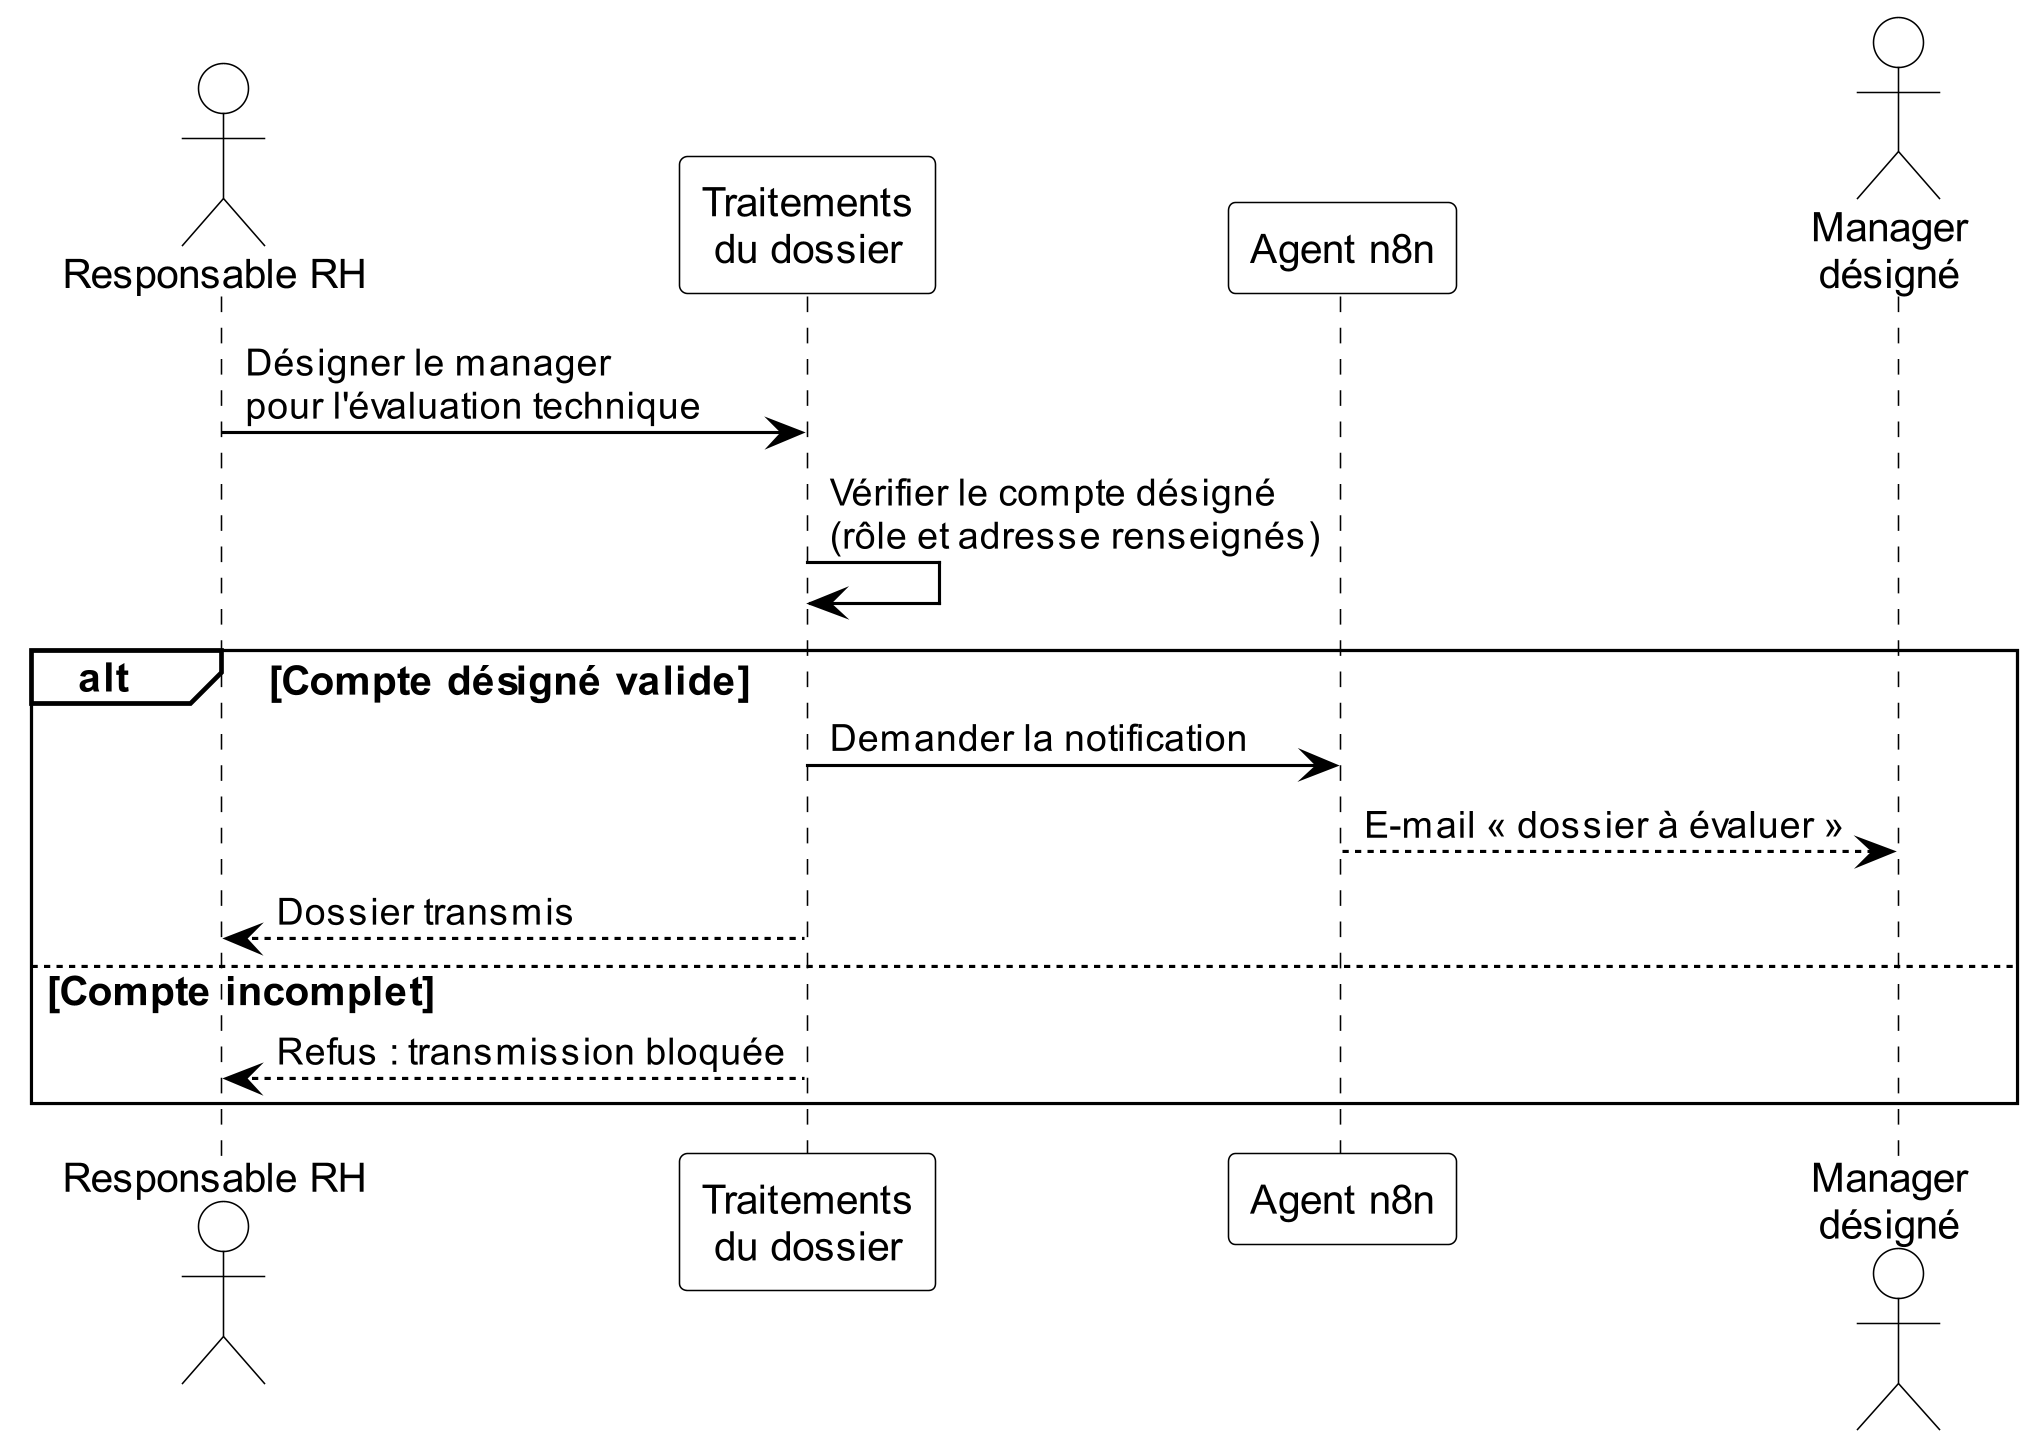
\includegraphics[width=\linewidth, height=0.94\textheight, keepaspectratio]{fig3_7b}
\caption{Diagramme de séquence objet — Routage des managers : notification du manager désigné}
\label{fig_3_7b}
\end{figure}
\endgroup

Les figures~\ref{fig_3_7a} et~\ref{fig_3_7b} détaillent destination et notification (section~\ref{sec_4_5_5}). La résolution du destinataire (manager de l’offre, puis département, puis famille de métier) ne produit plus qu’une proposition présélectionnée : le RH désigne, et le back-end refuse la transition sans désignation. Le compte choisi est gelé sur la candidature. Lui seul borne la visibilité du manager.

\section{Diagramme d’états — Cycle de vie d’une candidature}
\label{sec_3_6}
La figure~\ref{fig_3_8} donne la machine à états du dossier. Elle ne dessine que les transitions les plus représentatives ; les autres, autorisées par le garde-fou métier, sont détaillées dans la suite de cette section. Chaque statut y porte un libellé français, que le code rend par une constante — de \texttt{APPLIED} à \texttt{WITHDRAWN}, treize au total.

% figure 3.8
\setcounter{figure}{7}
\begin{figure}[!ht]
\centering
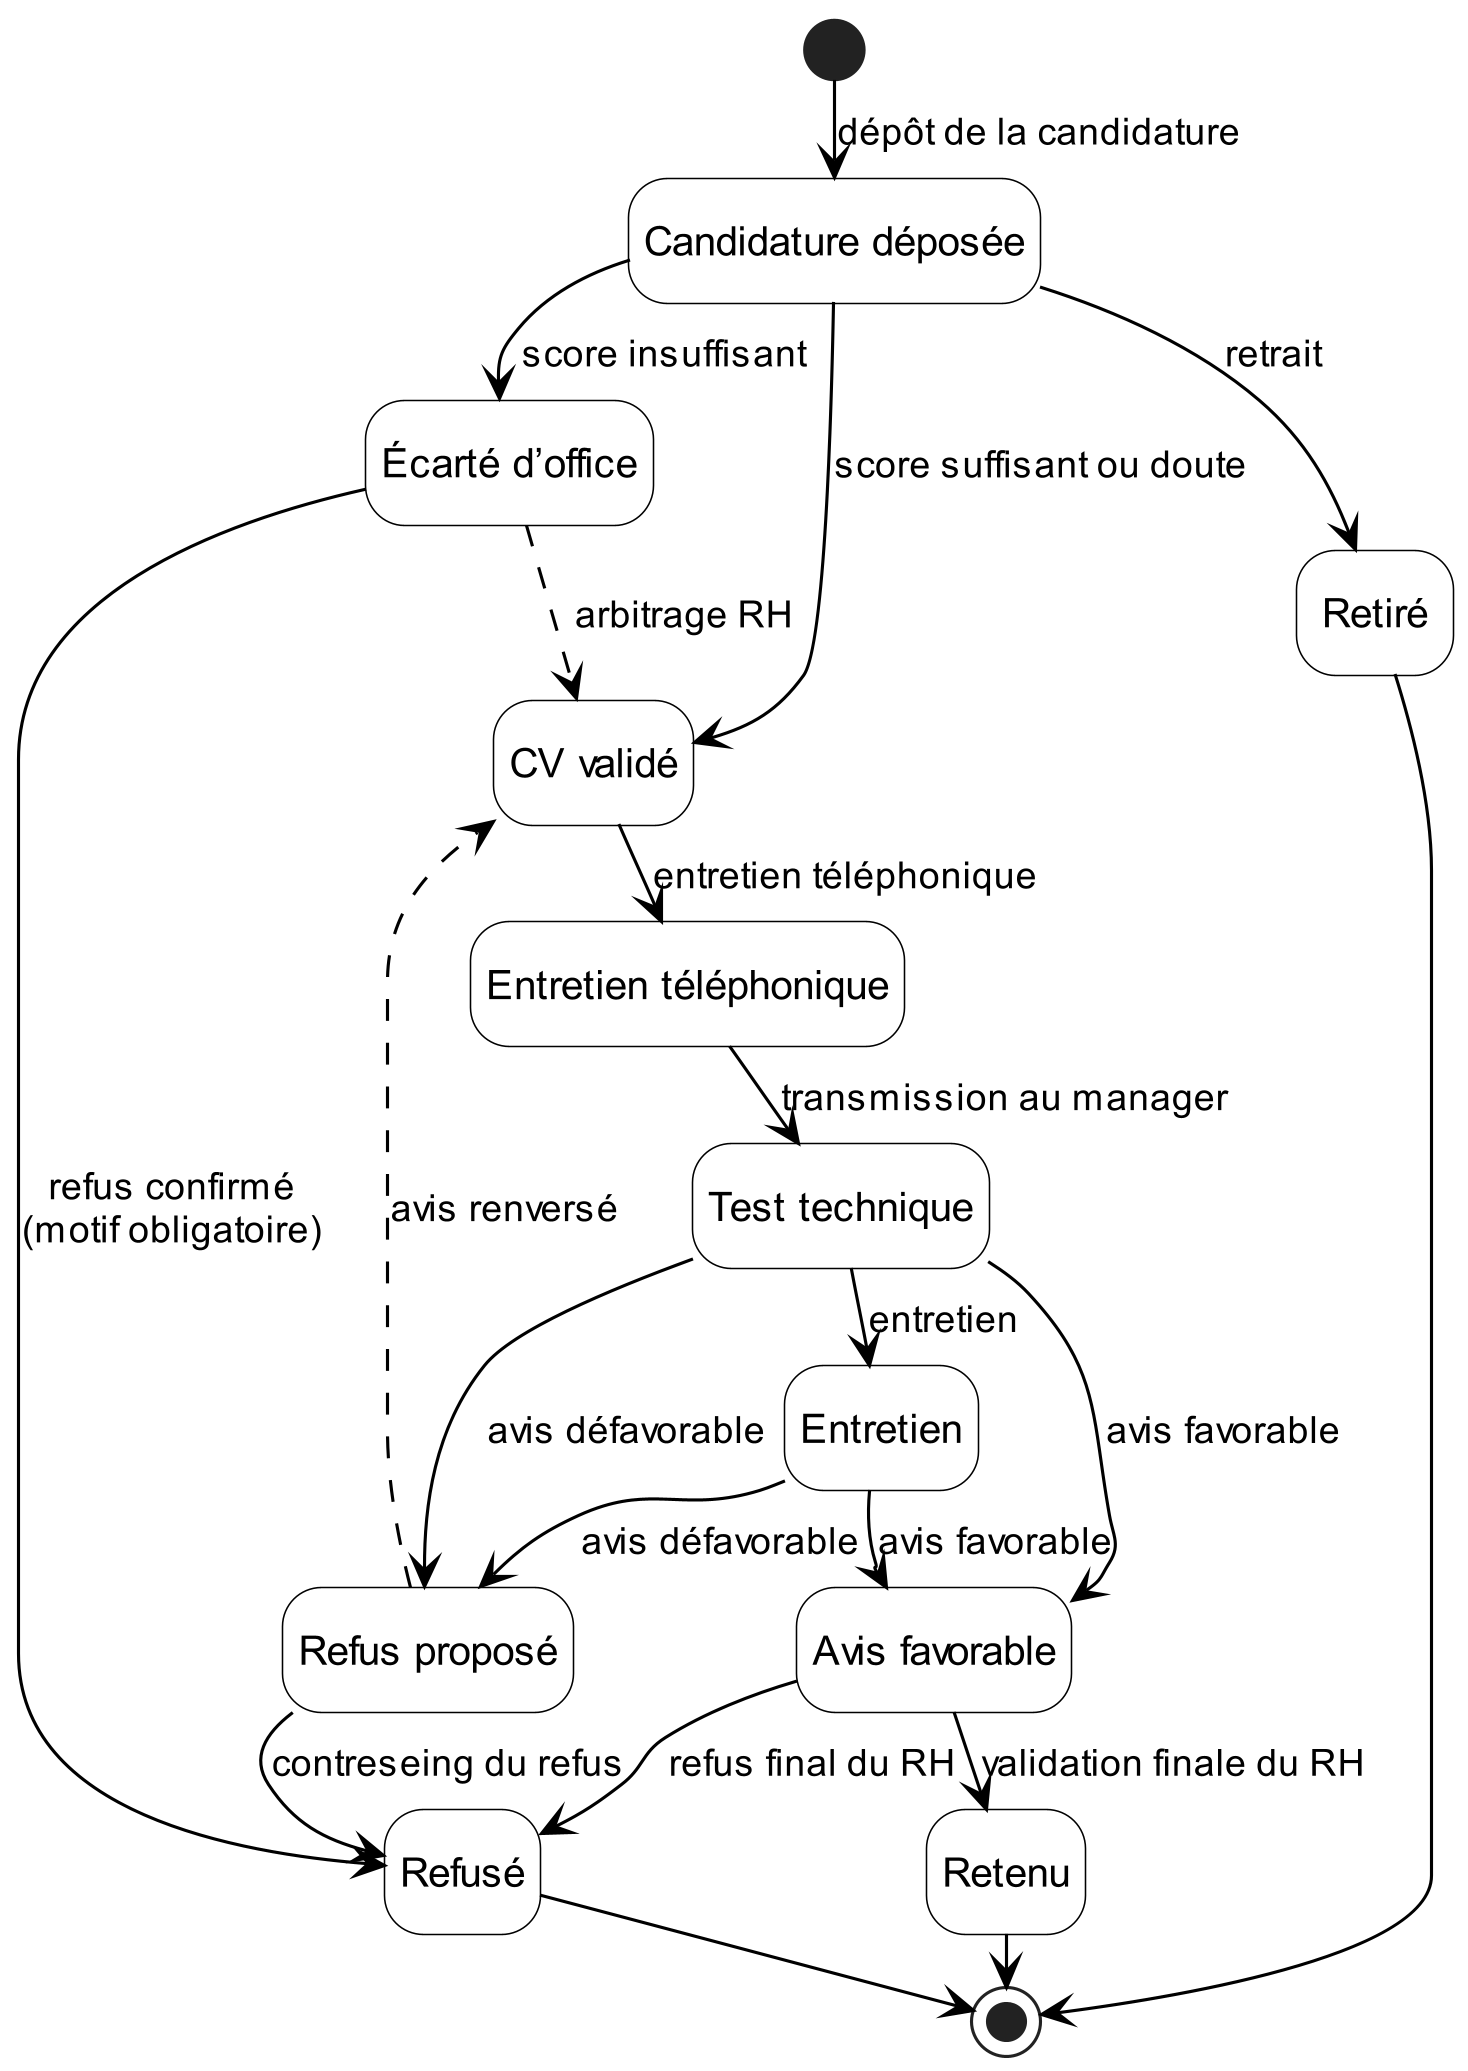
\includegraphics[width=\linewidth, height=0.94\textheight, keepaspectratio]{fig3_8}
\caption{Diagramme d’états du cycle de vie d’une candidature}
\label{fig_3_8}
\end{figure}

Le statut « entretien programmé » suit l’avis favorable : il matérialise la confirmation de l’agenda et précède la décision finale, sans désigner une étape d’évaluation. Planifier un entretien fait avancer le dossier à l’étape du type retenu (téléphonique, test, entretien, entretien final) ; si la machine à états refuse cette avancée, le dossier reste en place et l’entretien n’est pas annulé.

Un embranchement dépend du score : « CV validé » au-dessus du seuil du profil (60/100 par défaut), « écarté d’office » en dessous. Les dossiers signalés (CV inexploitable, écart de séniorité sévère, zone grise autour du seuil, service indisponible) échappent au rejet automatique et rejoignent l’examen humain (section~\ref{sec_4_4_6}). Le signalement et son motif, pas le statut, distinguent les deux cas.

La décision est à deux niveaux : avis du manager, puis contreseing du responsable RH. « Retenu » exige la date de présentation des documents, « refusé » exige un motif, et aucun des deux n’est atteint sans ce contreseing. Le RH peut aussi prononcer un refus final depuis n’importe quelle étape d’évaluation. Les trois états terminaux n’admettent plus aucune modification, mais « écarté d’office » reste entièrement révisable.

Deux garde-fous complètent cette décision, vérifiés par une série de refus contrôlés. D’abord « une personne, un poste » : l’identité retenue est l’adresse électronique assortie du prénom et du nom, et une personne déjà embauchée ne peut être embauchée une seconde fois ni déposer une nouvelle candidature. Les deux refus nomment l’offre et le dossier existants — « Cette personne est déjà embauchée sur l’offre … (dossier \#…) » côté RH, « Une personne en poste ne dépose pas de nouvelle candidature : contactez le RH si vous souhaitez changer de poste » côté candidat — pour que personne ne croie à une panne et ne représente le dossier ailleurs. Ensuite, un entretien ne peut être affecté qu’à un manager destinataire du dossier : le formulaire RH ne propose que ces destinataires, et le serveur refuse toute affectation extérieure à la création comme au changement de dossier ou d’intervieweur. Une affectation hors périmètre produirait en effet un entretien enregistré mais invisible dans le calendrier de ce manager, donc jamais conduit.

Ce rejet automatique n’a rien de définitif, ni d’entièrement hors de contrôle humain. À tout moment, le responsable RH ou l’administrateur dispose de deux issues :

\begin{itemize}
\item il confirme le refus après examen : le dossier passe à « refusé » avec un motif obligatoire, et le candidat ne reçoit pas de second e-mail, la notification ayant déjà été émise ;
\item il corrige manuellement le score : la justification est obligatoire et la correction est journalisée dans l’audit.
\end{itemize}

Dans ce second cas, le dossier reprend la règle de l’embranchement automatique. Une note corrigée à 60 ou plus le ramène au statut « CV validé » ; sous le seuil, une note corrigée replonge le dossier dans « écarté d’office ». La décision reste dans tous les cas humaine. Le score reste un filtre de présélection assisté. Il ne joue jamais le rôle d’une autorité décisionnelle.

Le cheminement d’une candidature se résume en six étapes :
\begin{itemize}
\item dépôt du CV et extraction de son texte par le back-end ;
\item mise en file d’attente puis déclenchement en arrière-plan de l’agent de lecture ;
\item rappel du back-end, qui interroge le service d’analyse et calcule le score sur 100 ;
\item au seuil, le dossier passe à « CV validé » ; sous le seuil, à « écarté d’office », sauf zone grise ou dossier signalé ;
\item arbitrage et correction du score possibles par le responsable RH ;
\item décision finale contresignée par le responsable RH, après avis du manager.
\end{itemize}

Le score ne provient pas d’une similarité vectorielle : la plateforme ne calcule aucun embedding ni distance cosinus et n’exécute aucun modèle local. La plupart des travaux sur l’appariement CV-offres reposent sur des plongements vectoriels \cite{ref22} ; ici, le score vient d’un modèle de langage, décomposé en trois critères lisibles.

Un unique message fixe le rôle du modèle, impose une sortie JSON à trois clés (technique, communication, séniorité) et interdit le zéro par défaut : faute d’information exploitable, le modèle renvoie 50. Il porte les trois champs descriptifs de l’offre et le texte intégral du CV. Les paramètres sont regroupés au tableau~\ref{tab_3_1}.

% tableau 3.1
\setcounter{table}{0}
\begin{table}[!ht]
\centering
\caption{Paramètres de l’appel d’analyse et de la décision automatique}
\label{tab_3_1}
\renewcommand{\arraystretch}{1.25}\footnotesize
\setlength{\tabcolsep}{4pt}%
\begin{tabular}{|P{0.30\textwidth}|P{0.65\textwidth}|}
\hline
\textbf{Paramètre} & \textbf{Valeur retenue} \\
\hline
Modèle et service & command-a-03-2025, servi par l’API de Cohere \\
\hline
Température, longueur & nulle, 200 jetons au plus \\
\hline
Sortie exigée & JSON à trois clés : technique, communication, séniorité \\
\hline
Valeur de repli & 50 sur les trois clés si l’information est inexploitable \\
\hline
Score final & moyenne pondérée arrondie sur 100 \\
\hline
Poids par défaut & 0,5 / 0,2 / 0,3 ; somme contrôlée à $\pm$0,01 près \\
\hline
Profils de pondération & douze profils (table \texttt{scoring\_weight\_profiles}), choisis par famille de métier et niveau de séniorité \\
\hline
Seuil de décision & 60/100 par défaut, calibrable profil par profil sur le Gold Set (\texttt{decision\_threshold}) \\
\hline
Zone grise d’arbitrage & cinq points au-dessous ou au-dessus du seuil du profil \\
\hline
\end{tabular}
\end{table}

La réponse est relue côté serveur : le bloc JSON est extrait du texte, « 86/100 » devient 86 et le résultat est borné entre 0 et 100. Si une clé manque ou reste illisible, l’appel échoue et le mode dégradé local prend le relais avec un score marqué « simulé » (section~\ref{sec_4_4_6}). La valeur neutre de 50 n’est qu’une consigne du prompt : rien n’est inventé.

Le score sur 100 est la moyenne pondérée des trois critères, aux poids du profil de famille de métier et de séniorité : 80, 70 et 60 donnent 72 aux poids par défaut. Les compétences retenues ne viennent pas du modèle mais d’un calcul local par dictionnaire d’alias.

Ce choix répond d’abord à une contrainte d’environnement. L’inférence hébergée sur Hugging Face était bloquée par la politique réseau de l’entreprise ; le point d’entrée de Cohere a été vérifié accessible, et le service reste managé, sans GPU ni poids de modèle à déployer. Un modèle embarqué du type sentence-transformers aurait exigé une infrastructure d’exécution et un entraînement adaptés au français des offres.

Deux réserves sont assumées. La sortie JSON contrainte et la température nulle réduisent la variabilité sans garantir une reproductibilité parfaite, le modèle comme le service pouvant évoluer. La version du modèle, celle du prompt et la réponse brute ne sont pas encore archivées : cet enregistrement reste à prévoir pour rendre une évaluation réellement rejouable.

\section{Conception de la base de données}
\label{sec_3_7}
La base PostgreSQL reflète directement le diagramme de classes de la section~\ref{sec_3_3}. Chaque entité JPA est mappée sur une table, et les relations One-to-Many et Many-to-One deviennent des clés étrangères : \texttt{job\allowbreak\_offers\allowbreak.hiring\allowbreak\_manager\allowbreak\_id}, \texttt{candidates\allowbreak.routed\allowbreak\_to\allowbreak\_manager\allowbreak\_id}, \texttt{interviews\allowbreak.candidate\allowbreak\_id}, \texttt{feedbacks\allowbreak.interview\allowbreak\_id}.

J’ai configuré la génération du schéma en mode «~update~» (Hibernate ddl-auto), pratique en développement pour faire évoluer la structure sans perte de données. En production, ce mode devrait céder la place à des migrations versionnées (Flyway ou Liquibase), seules capables de garantir des évolutions maîtrisées.

Le schéma présente les tables générées à partir des entités JPA, découpées par domaine pour rester lisibles à l’impression. Comptes et référentiel figurent sur la figure~\ref{fig_3_9}, dossiers et CV sur la figure~\ref{fig_3_9a}. Offres, entretiens et retours d’évaluation viennent en figure~\ref{fig_3_9b}, audit, rappels et file d’attente n8n en figures~\ref{fig_3_9c} et~\ref{fig_3_9d}.

% figure 3_9
\setcounter{figure}{8}
\begin{figure}[!ht]
\centering
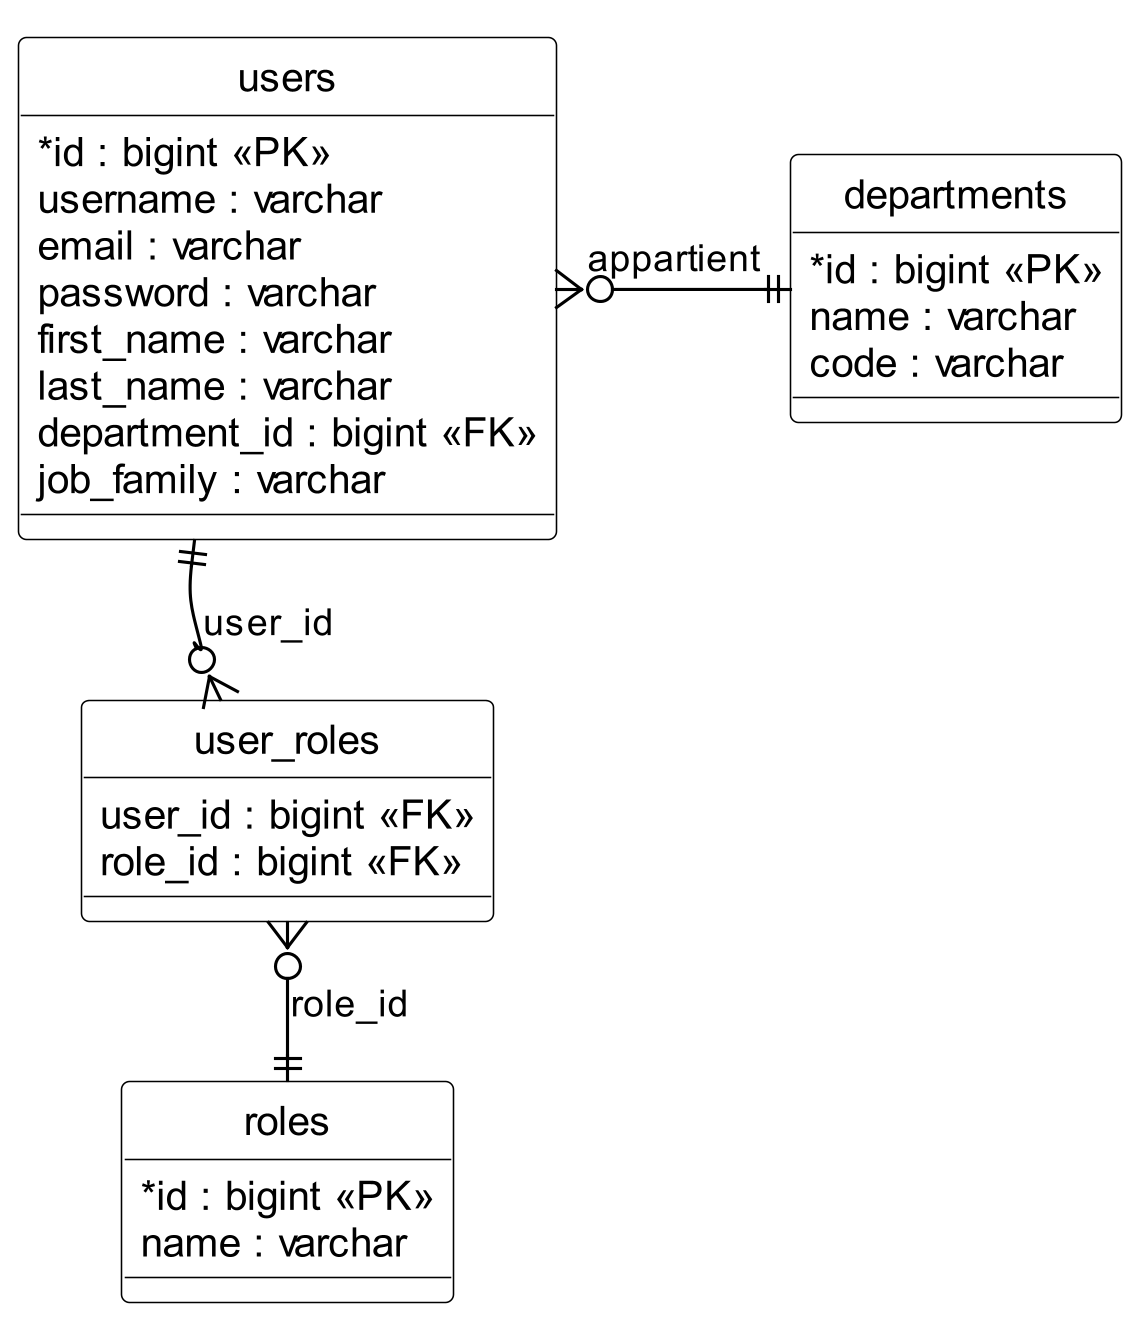
\includegraphics[width=355pt, keepaspectratio]{fig3_9}
\caption{Schéma relationnel — comptes, rôles et départements}
\label{fig_3_9}
\end{figure}

% figure 3_9
\setcounter{figure}{8}
\begingroup\renewcommand{\thefigure}{3.9a}
\begin{figure}[!ht]
\centering
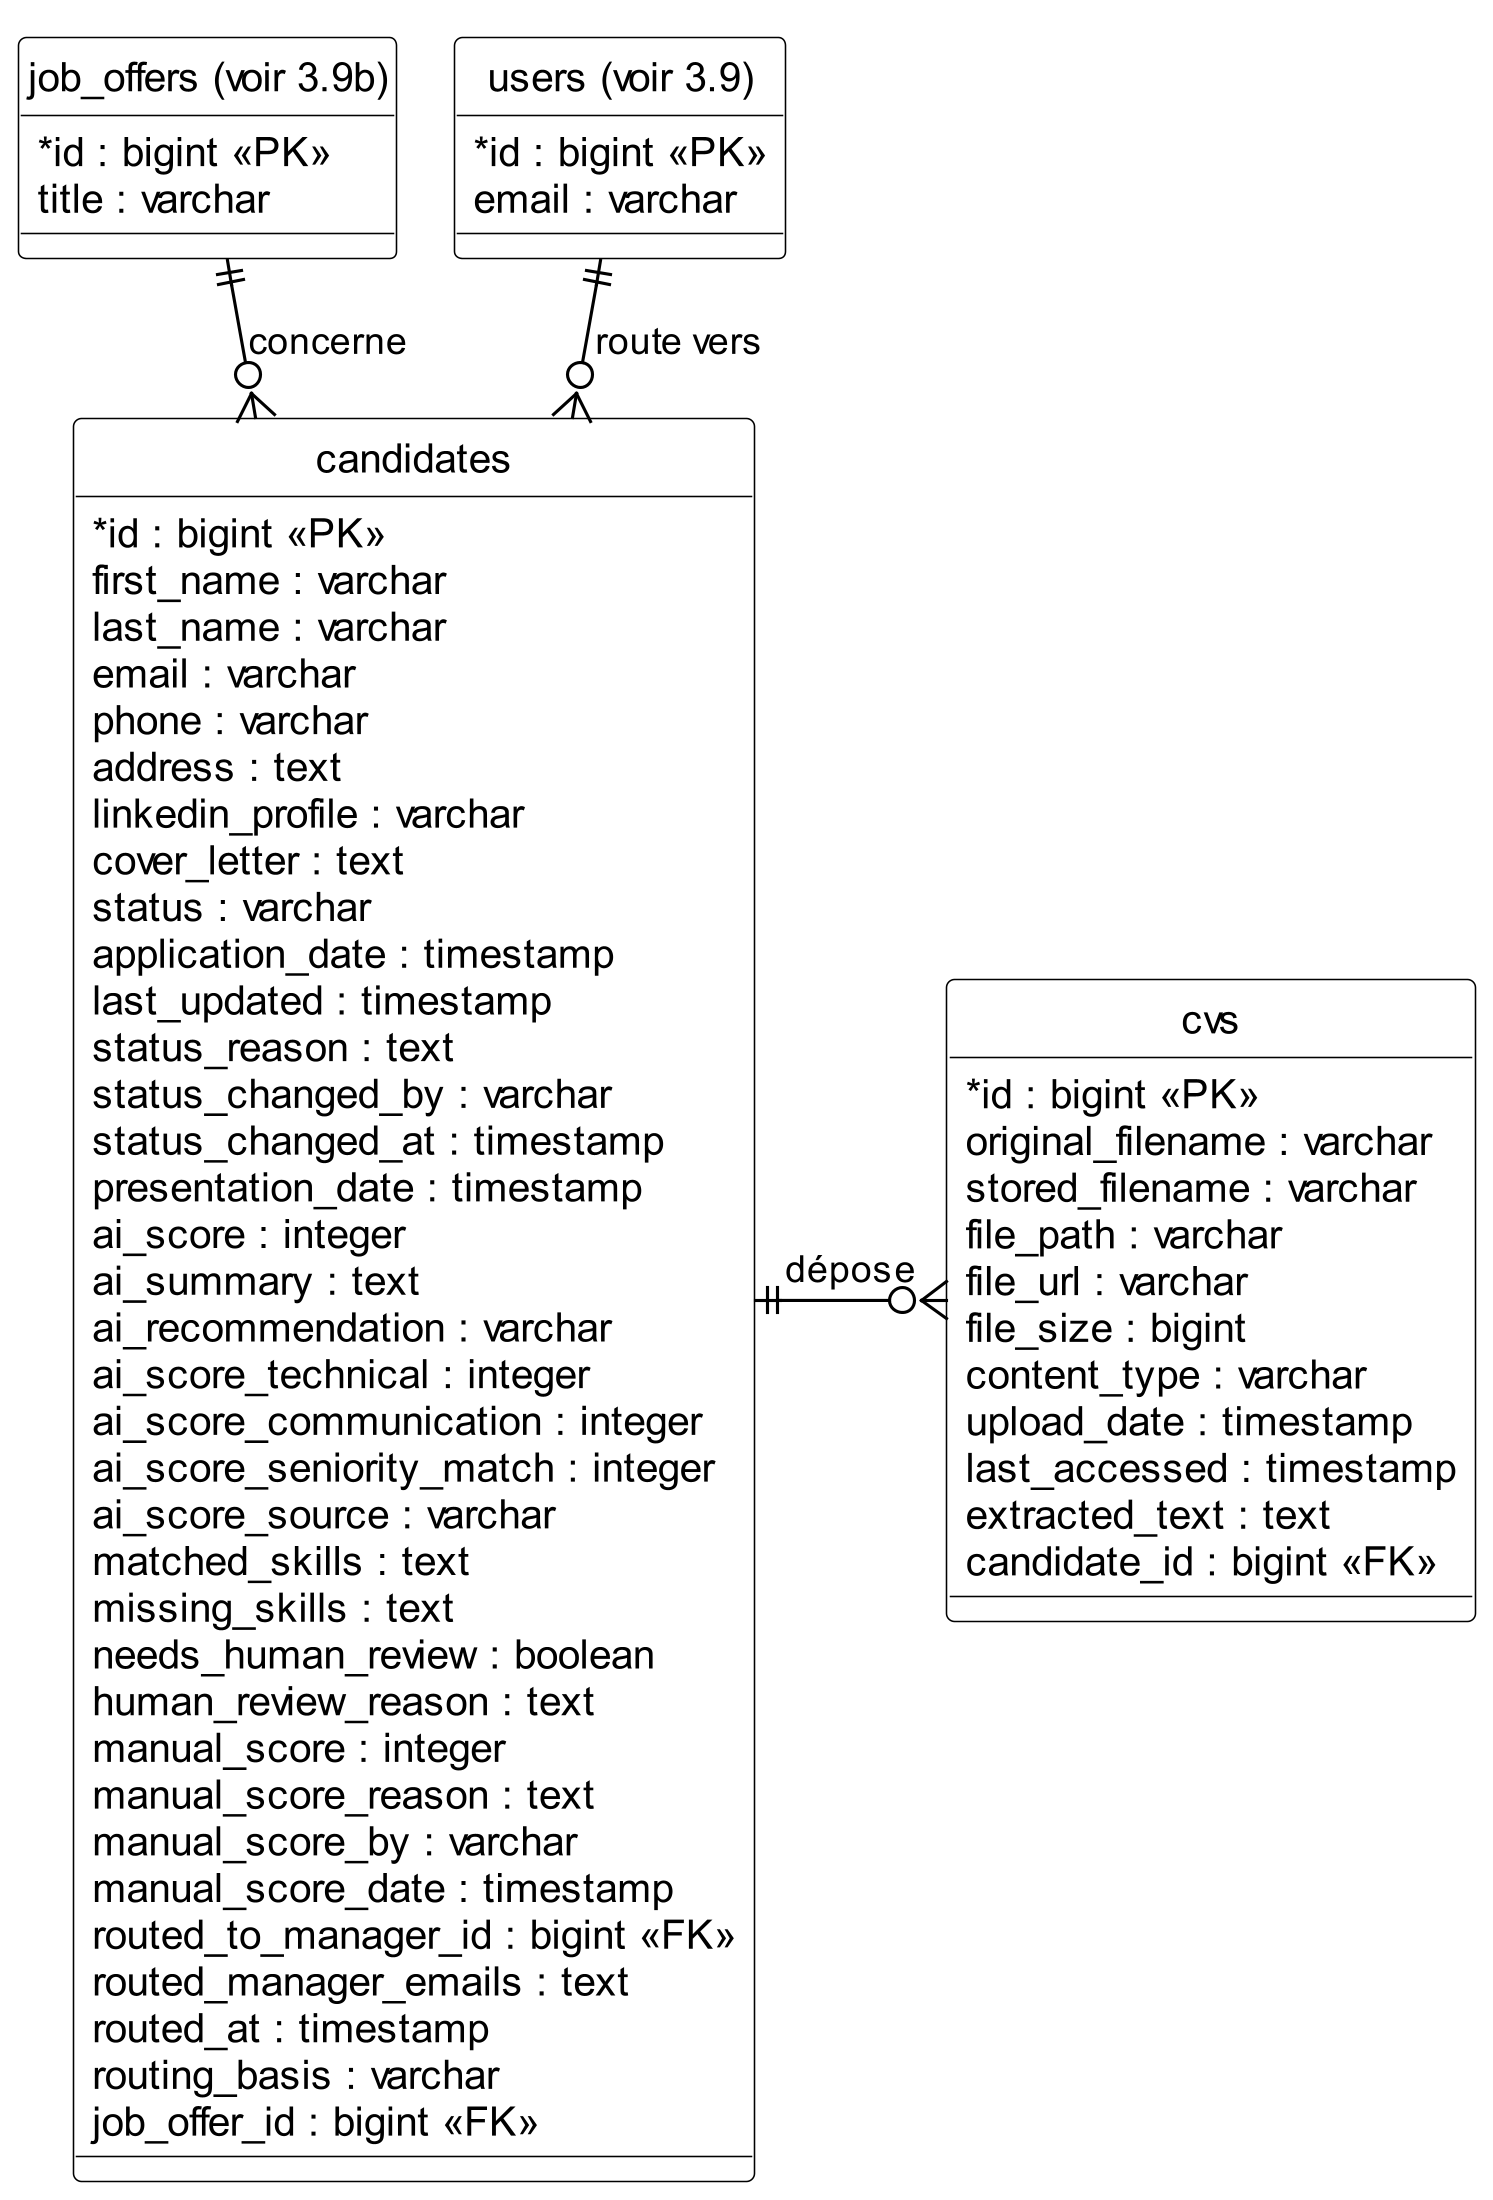
\includegraphics[width=\linewidth, height=0.94\textheight, keepaspectratio]{fig3_9a}
\caption{Schéma relationnel — dossiers de candidature et CV}
\label{fig_3_9a}
\end{figure}
\endgroup

% figure 3_9
\setcounter{figure}{8}
\begingroup\renewcommand{\thefigure}{3.9b}
\begin{figure}[!ht]
\centering
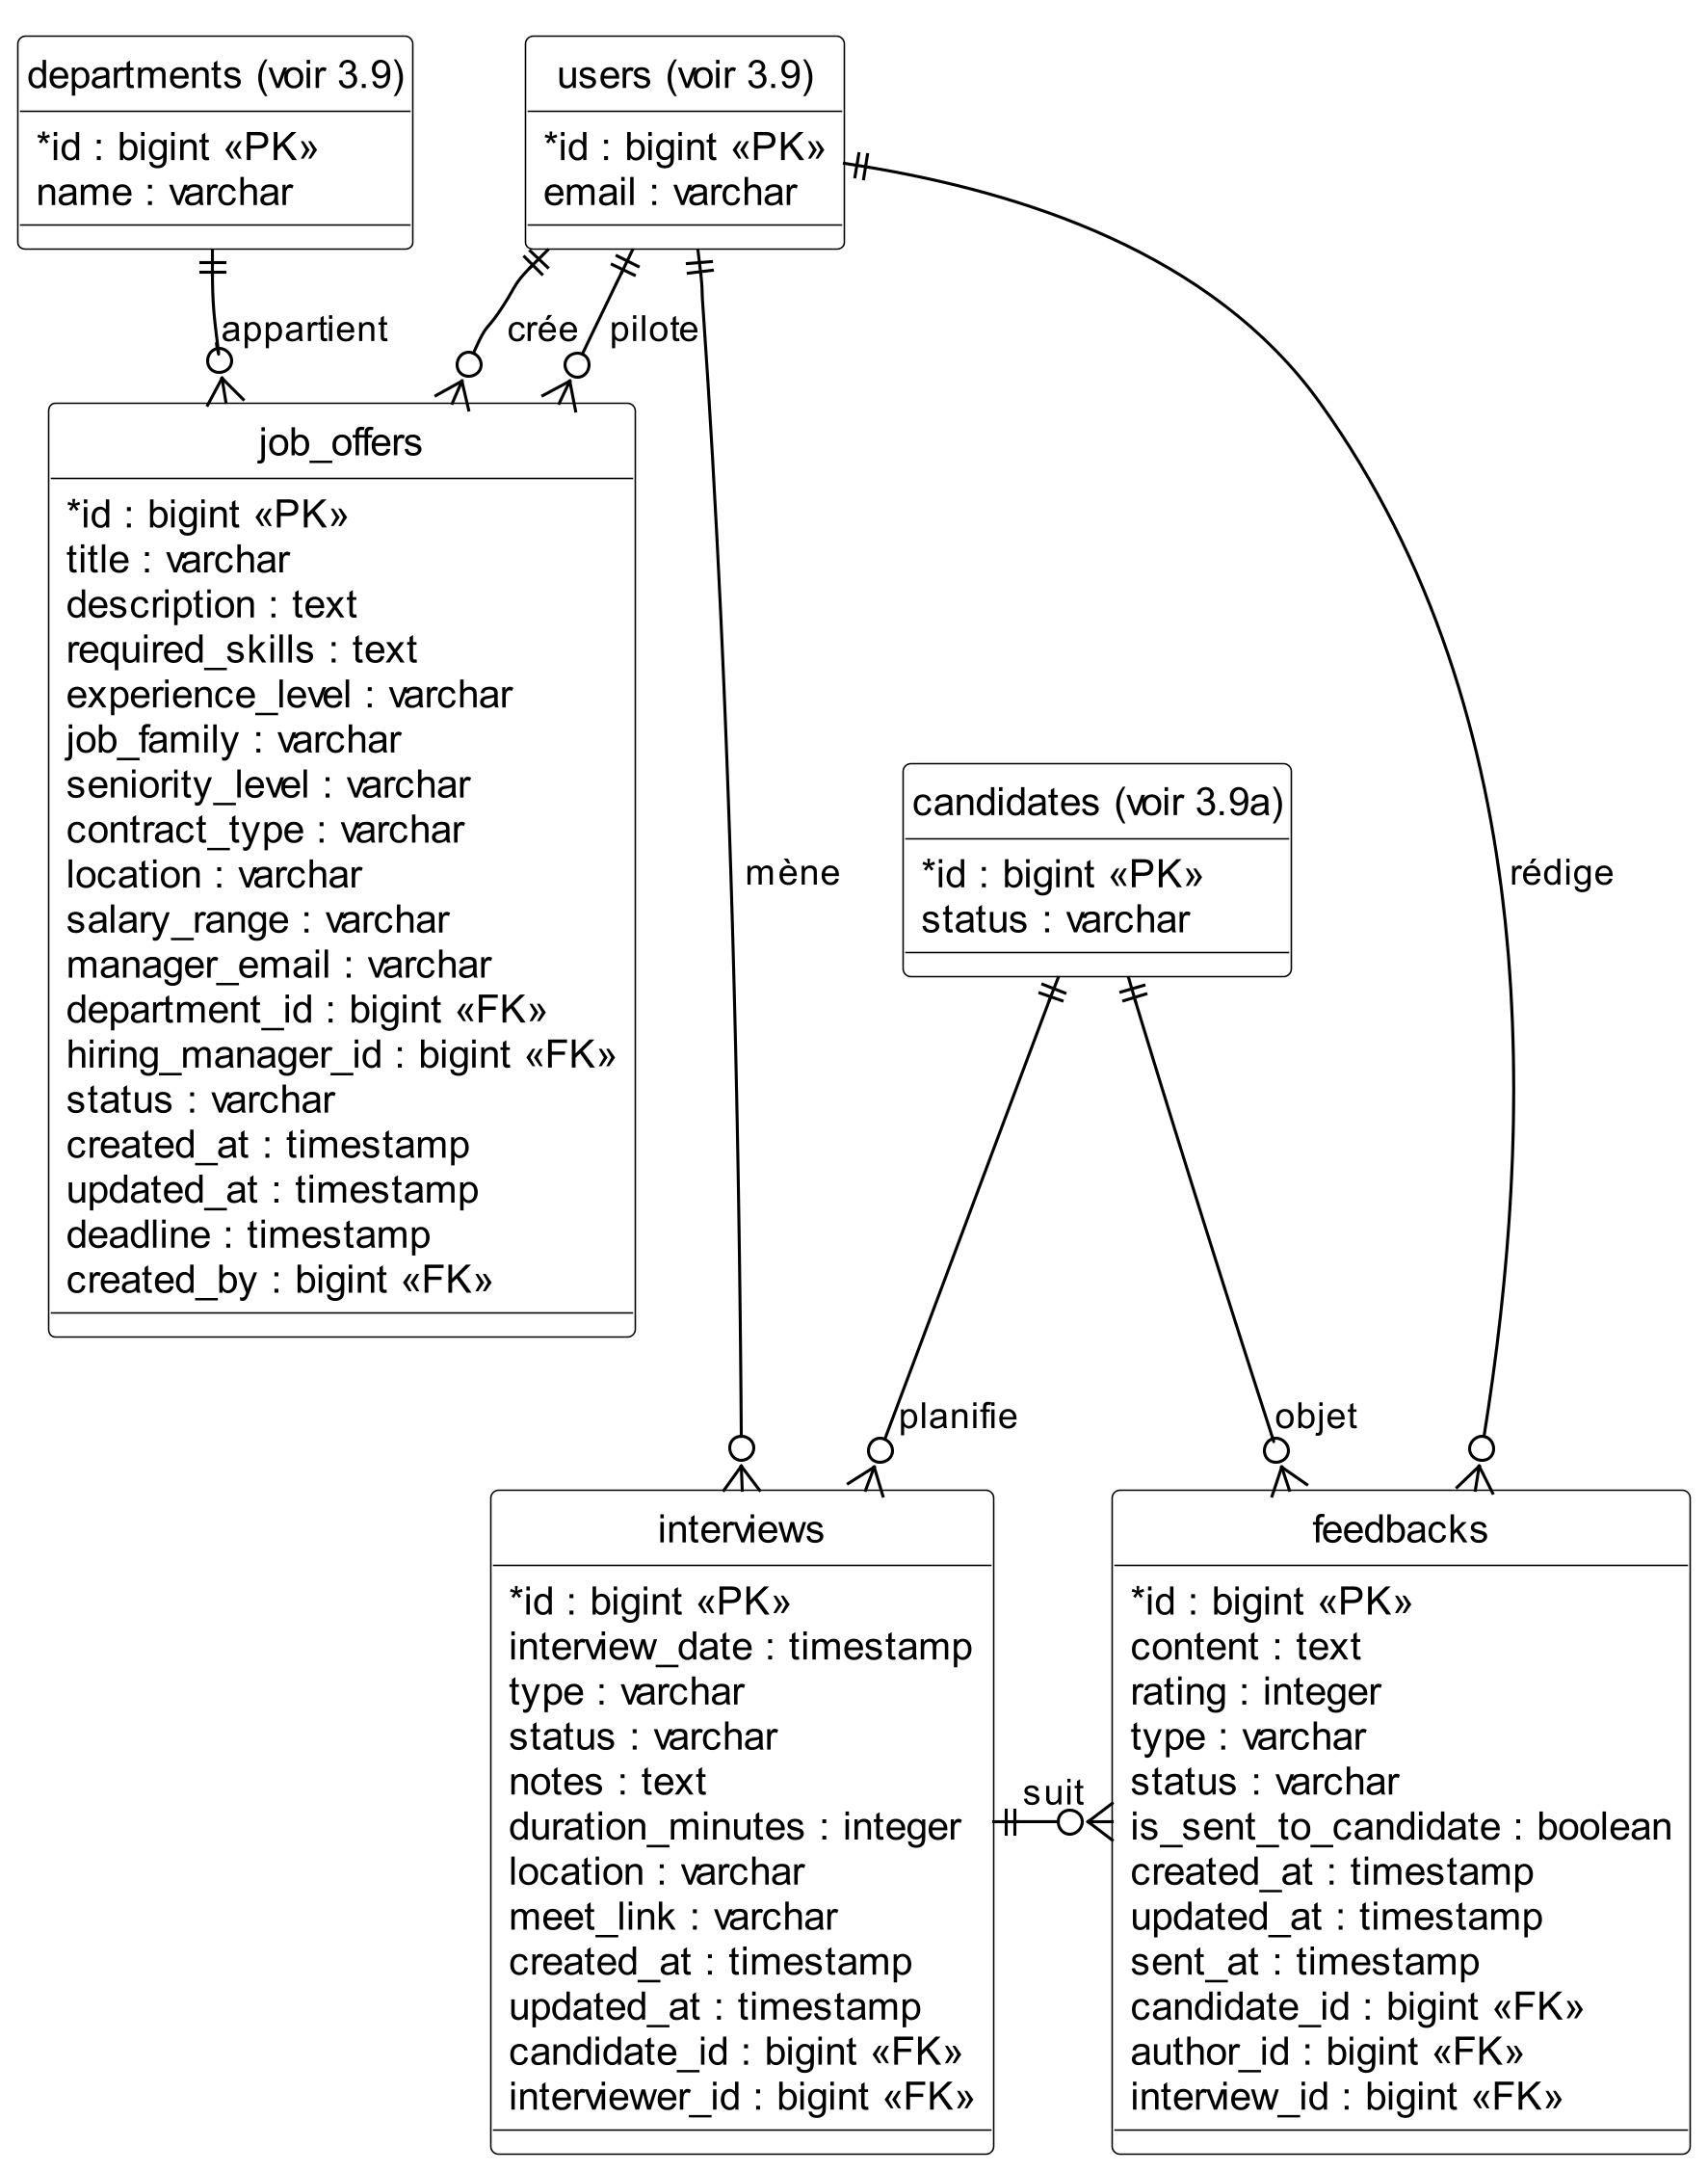
\includegraphics[width=\linewidth, height=0.94\textheight, keepaspectratio]{fig3_9b}
\caption{Schéma relationnel — offres, entretiens et retours d’évaluation}
\label{fig_3_9b}
\end{figure}
\endgroup

% figure 3_9
\setcounter{figure}{8}
\begingroup\renewcommand{\thefigure}{3.9c}
\begin{figure}[!ht]
\centering
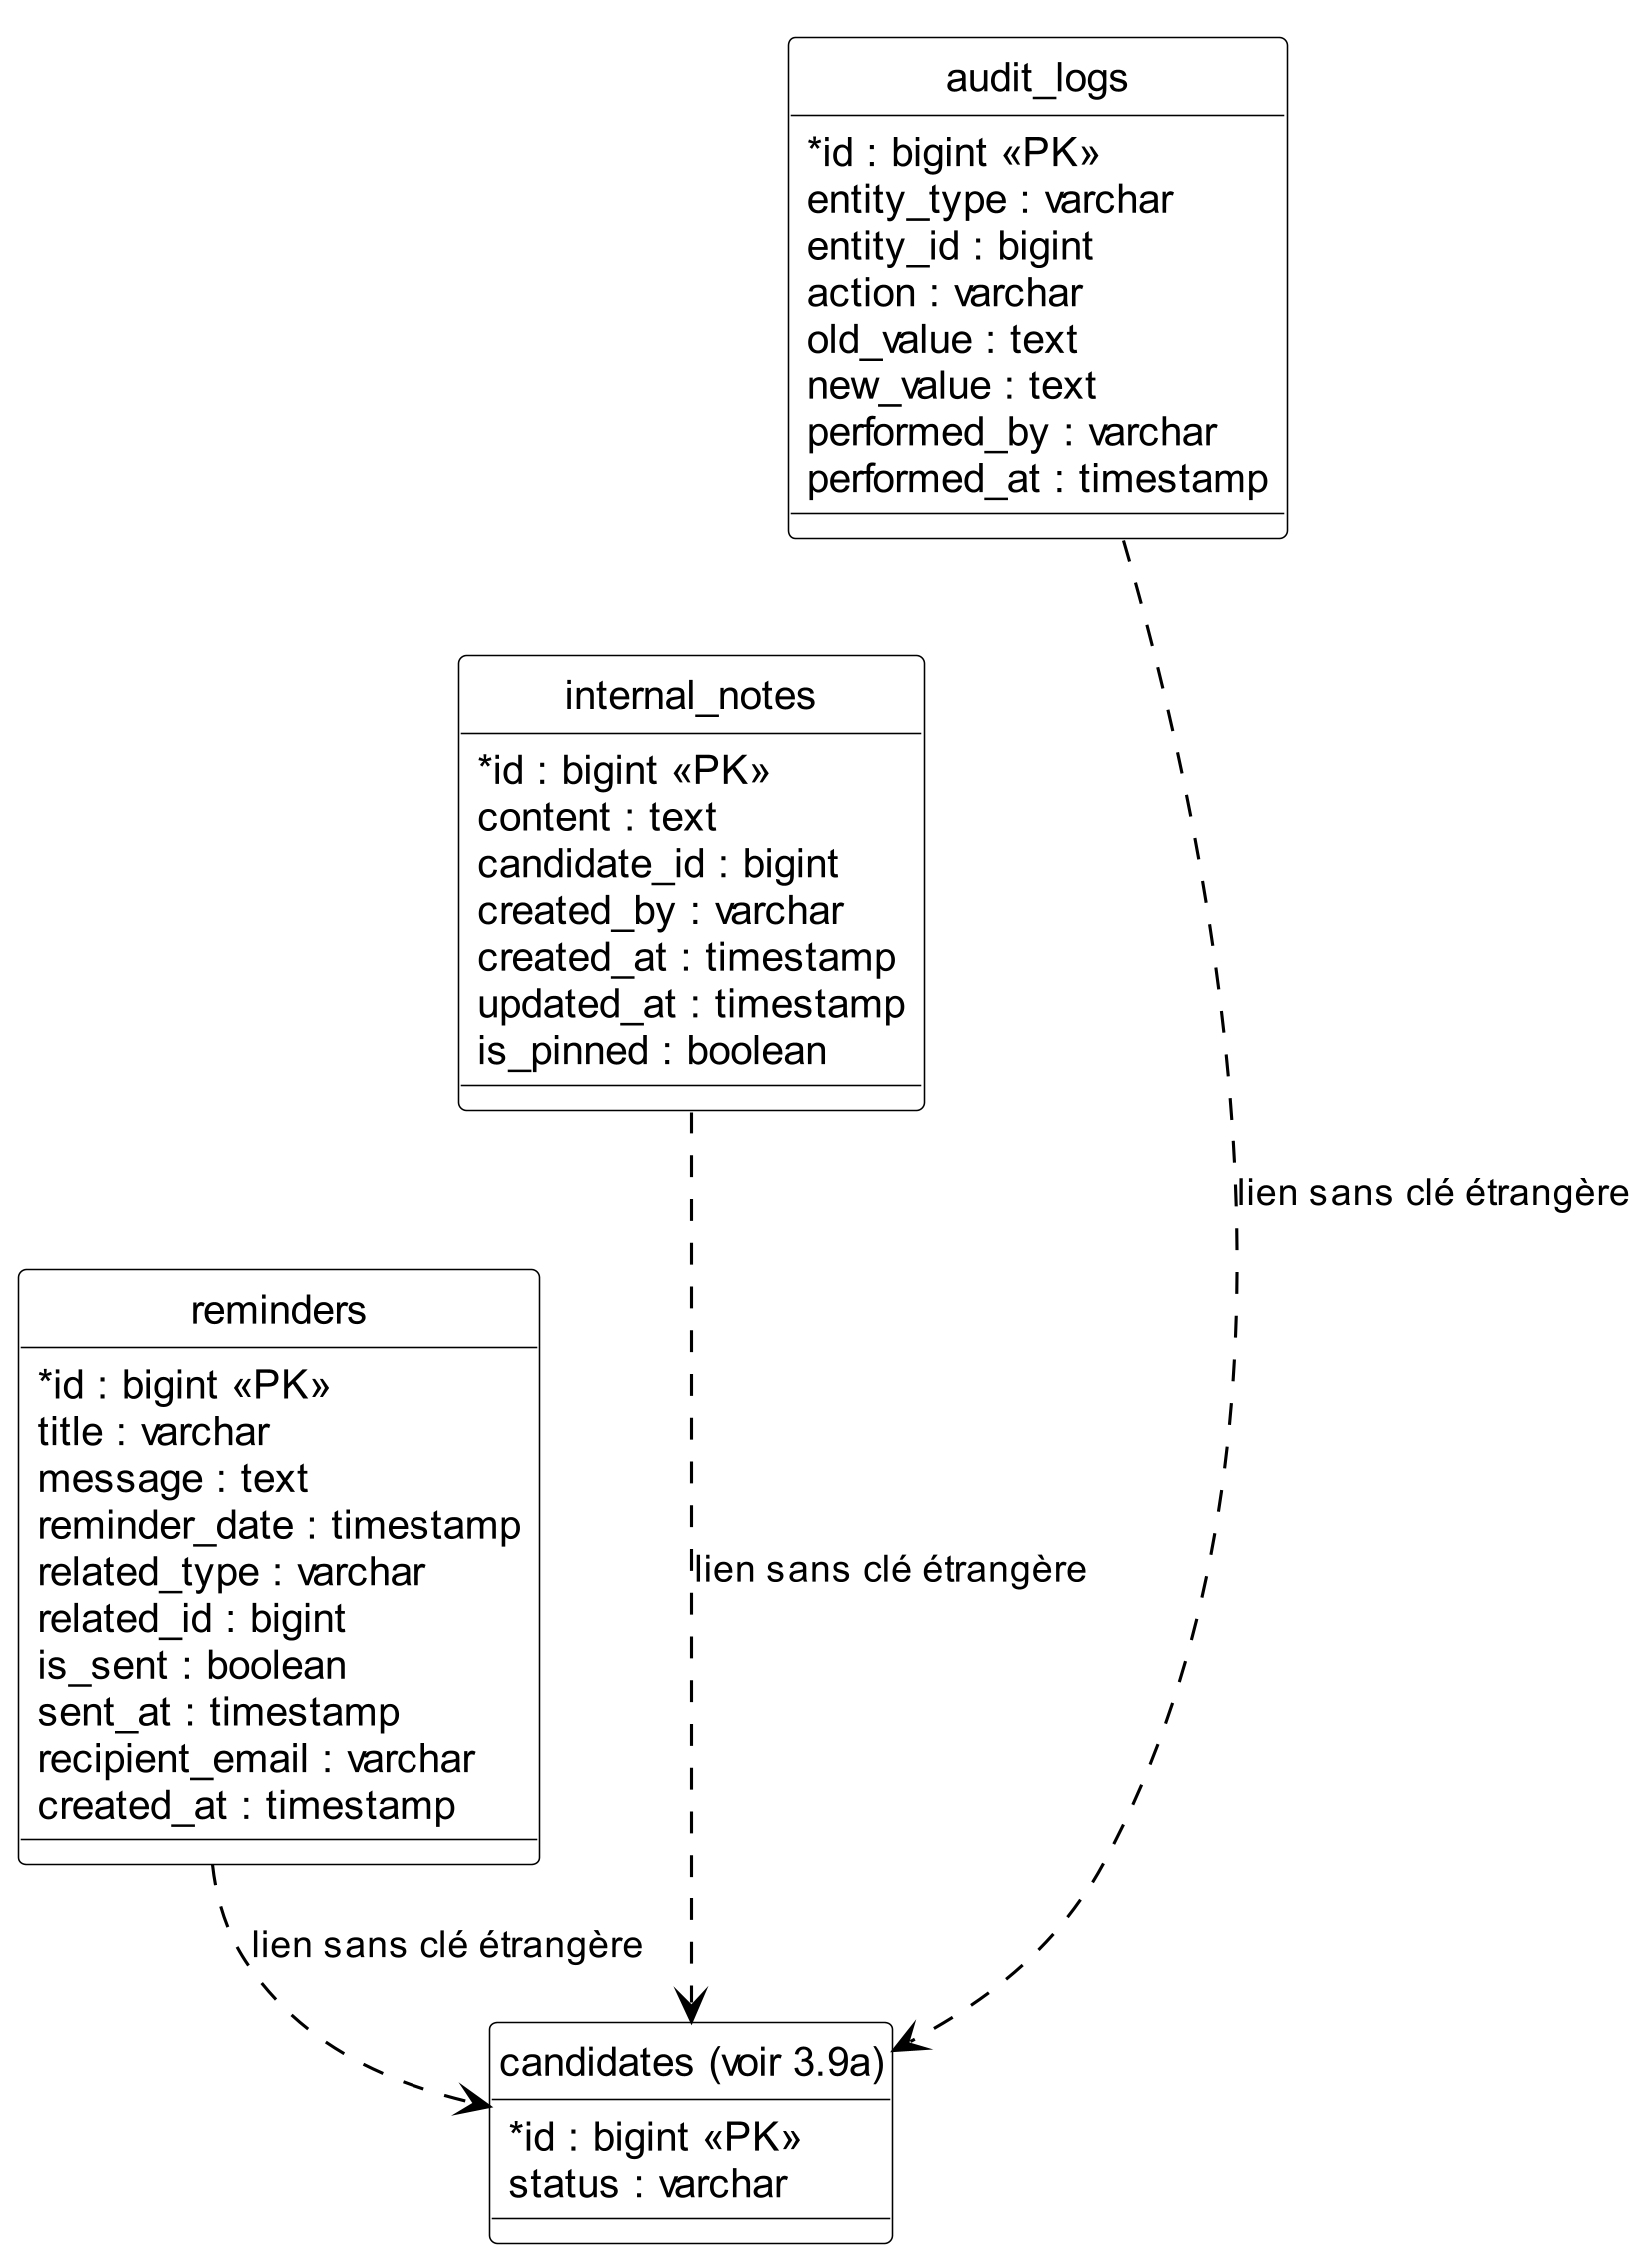
\includegraphics[width=\linewidth, height=0.94\textheight, keepaspectratio]{fig3_9c}
\caption{Schéma relationnel — audit, notes internes et rappels}
\label{fig_3_9c}
\end{figure}
\endgroup

% figure 3_9
\setcounter{figure}{8}
\begingroup\renewcommand{\thefigure}{3.9d}
\begin{figure}[!ht]
\centering
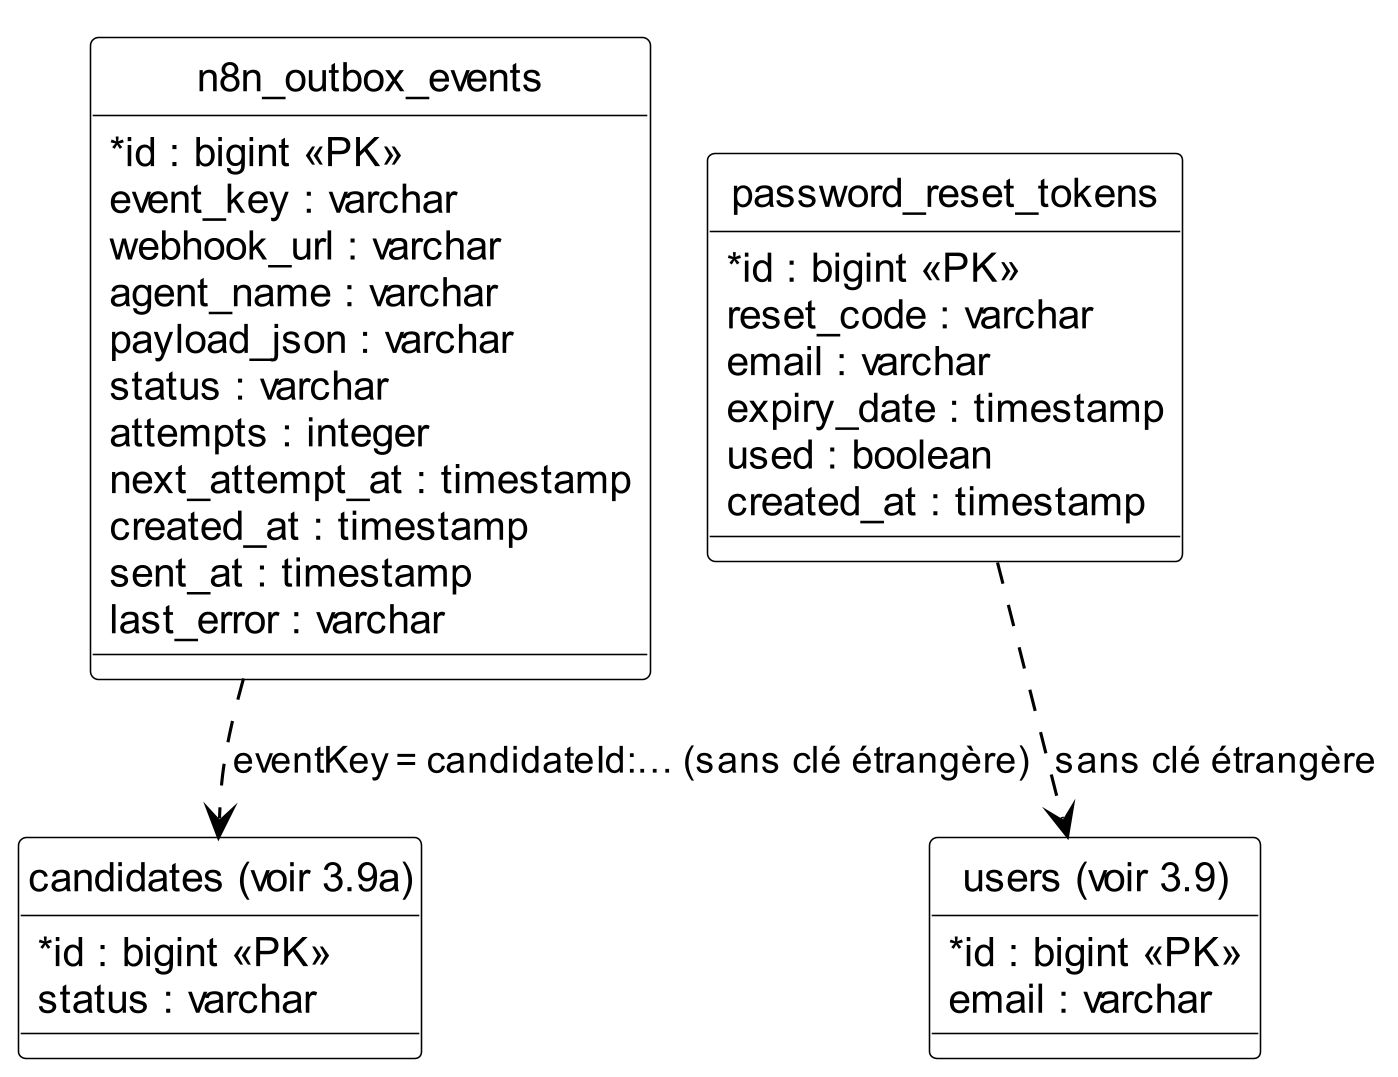
\includegraphics[width=440pt, keepaspectratio]{fig3_9d}
\caption{Schéma relationnel — file d’attente n8n et jetons de réinitialisation}
\label{fig_3_9d}
\end{figure}
\endgroup

Le schéma reprend fidèlement les entités JPA : clé primaire signalée par un astérisque et le stéréotype \texttt{<<PK>>}, clé étrangère par \texttt{<<FK>>}, cardinalités en patte de poule. On y lit les relations structurantes (département, offres, candidatures, CV, entretiens, retours) et la destination du routage, figée sur le dossier (\texttt{routed\_to\_manager\_id}, \texttt{routing\_basis}).

Quatre liens suivis par le code n’ont, en revanche, pas de clé étrangère en base, et apparaissent à ce titre en pointillés :

\begin{itemize}
\item le jeton de réinitialisation se rattache à un compte par son adresse e-mail ;
\item la file n8n, les rappels et les notes internes se rattachent à un dossier par une colonne conventionnelle (\texttt{event\_key}, \texttt{related\_id}, \texttt{candidate\_id}) que Hibernate ne contraint pas.
\end{itemize}

Ce choix est assumé : ces tables doivent survivre à la suppression éventuelle de la ligne qu’elles décrivent et restent interrogeables sans jointure. Les tables rappelées en tête de panneau avec la mention «~détail fig.~» n’y figurent qu’en référence, avec leur clé et leur clé naturelle ; leurs colonnes complètes sont listées sur le panneau de leur domaine.

\section{Diagramme de composants}
\label{sec_3_8}
Le diagramme de la figure~\ref{fig_3_10} détaille l’organisation de la plateforme en deux composants déployables (le front-end Angular et le back-end Spring Boot) et leurs dépendances. La flèche pleine marque une dépendance d’exécution, l’émetteur appelant le récepteur ; la flèche pointillée marque une collaboration transversale qui n’immobilise pas l’appelant : le filtrage des routes côté front, l’authentification côté back et la journalisation des actions.

% figure 3.10
\setcounter{figure}{9}
\begin{landscape}
\pagestyle{lscape}
\begin{figure}[p]
\centering
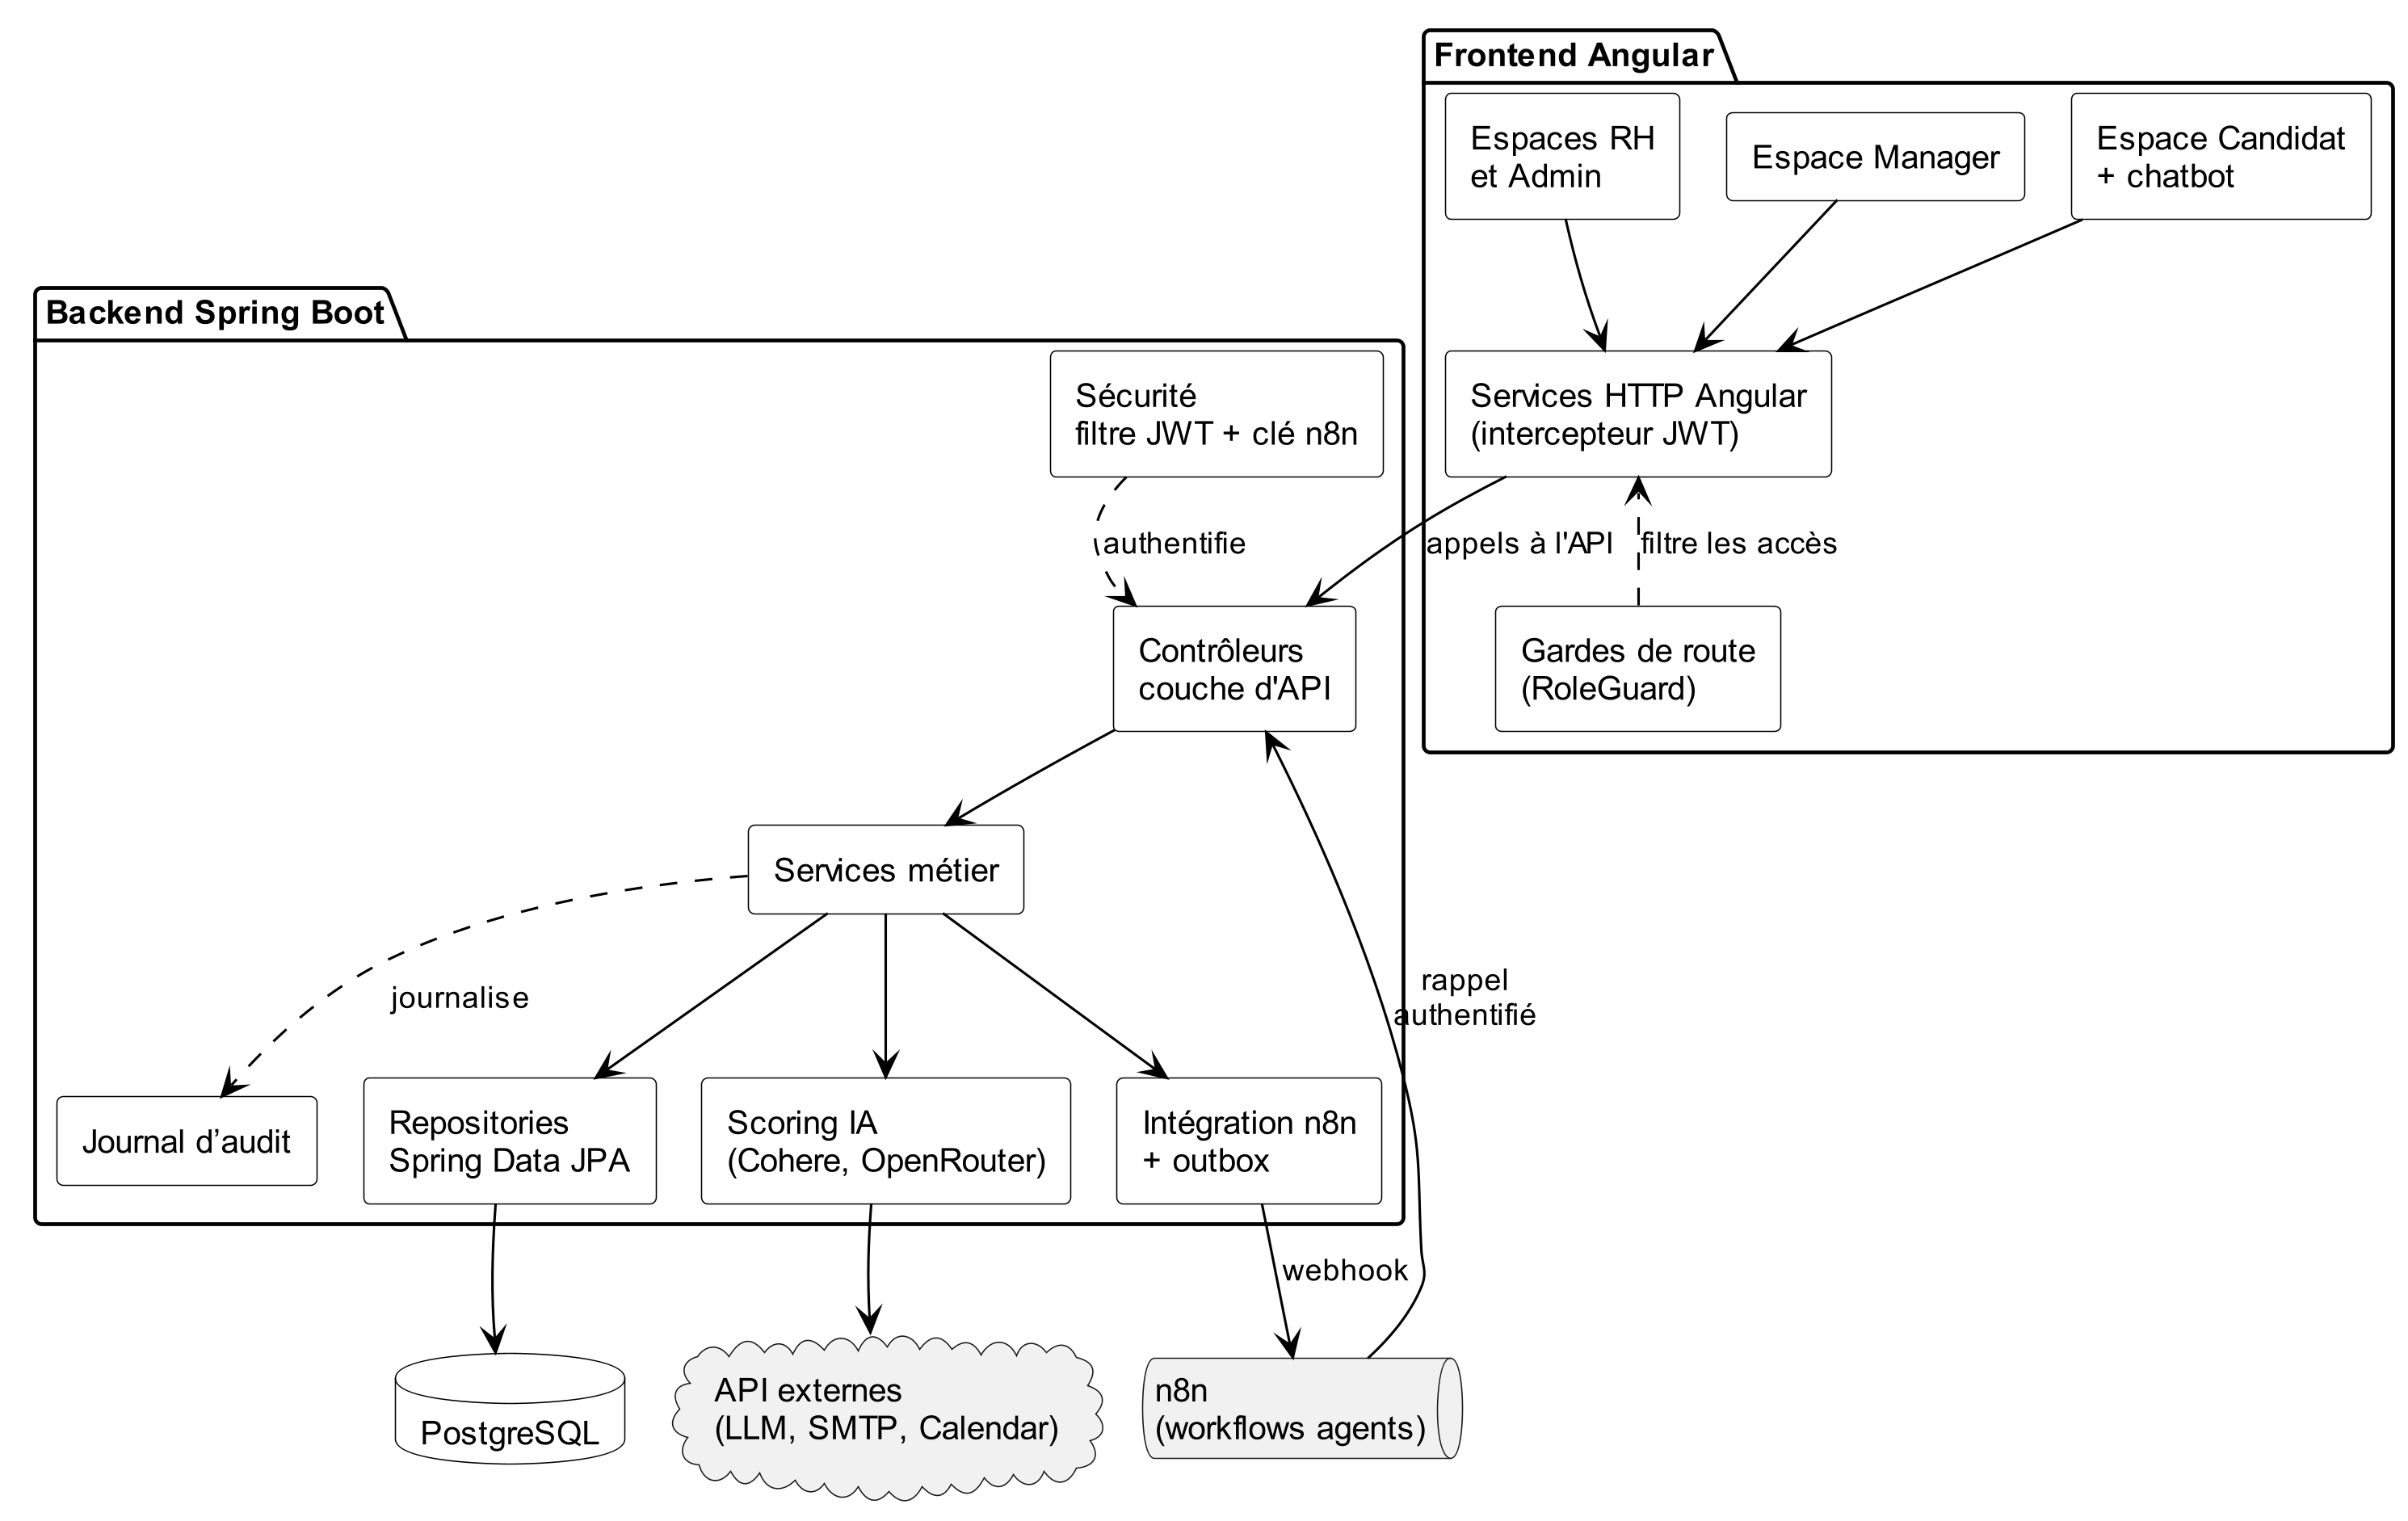
\includegraphics[width=0.98\linewidth, height=0.92\textheight, keepaspectratio]{fig3_10}
\caption{Diagramme de composants de la plateforme JOB4YOU}
\label{fig_3_10}
\end{figure}
\clearpage
\end{landscape}

Le front-end ne touche jamais la base : ses services HTTP, portés par l’intercepteur JWT, adressent la seule surface d’entrée du back-end, ses points d’entrée REST.

Deux gardes complètent le dispositif : les \texttt{RoleGuard} angular masquent les routes qu’un rôle n’a pas le droit d’emprunter, et le filtre Spring (jeton JWT pour les utilisateurs, clé d’API pour n8n) authentifie la requête avant qu’elle n’atteigne la couche métier.

Chaque service métier (Candidate, Interview, Feedback, JobOffer) s’appuie alors sur la couche de repositories Spring Data JPA pour la persistance, et sur le service d’audit pour tracer les actions sensibles. Le service Candidate délègue le calcul du score au service de scoring IA, qui appelle les fournisseurs externes.

Candidate et Interview déclenchent chacun les agents n8n compétents via la table d’attente, et le retour de l’agent (recalcul du score, notification) reprend l’entrée du back-end par un rappel authentifié. Ce dernier aller-retour donne au diagramme sa forme en boucle : le back-end y est à la fois appelant et rappelé.

\section{Diagramme de déploiement}
\label{sec_3_9}
Le diagramme de la figure~\ref{fig_3_11} représente la répartition physique des composants de la plateforme JOB4YOU sur les nœuds d’exécution, ainsi que leurs protocoles de communication.

% figure 3.11
\setcounter{figure}{10}
\begin{landscape}
\pagestyle{lscape}
\begin{figure}[p]
\centering
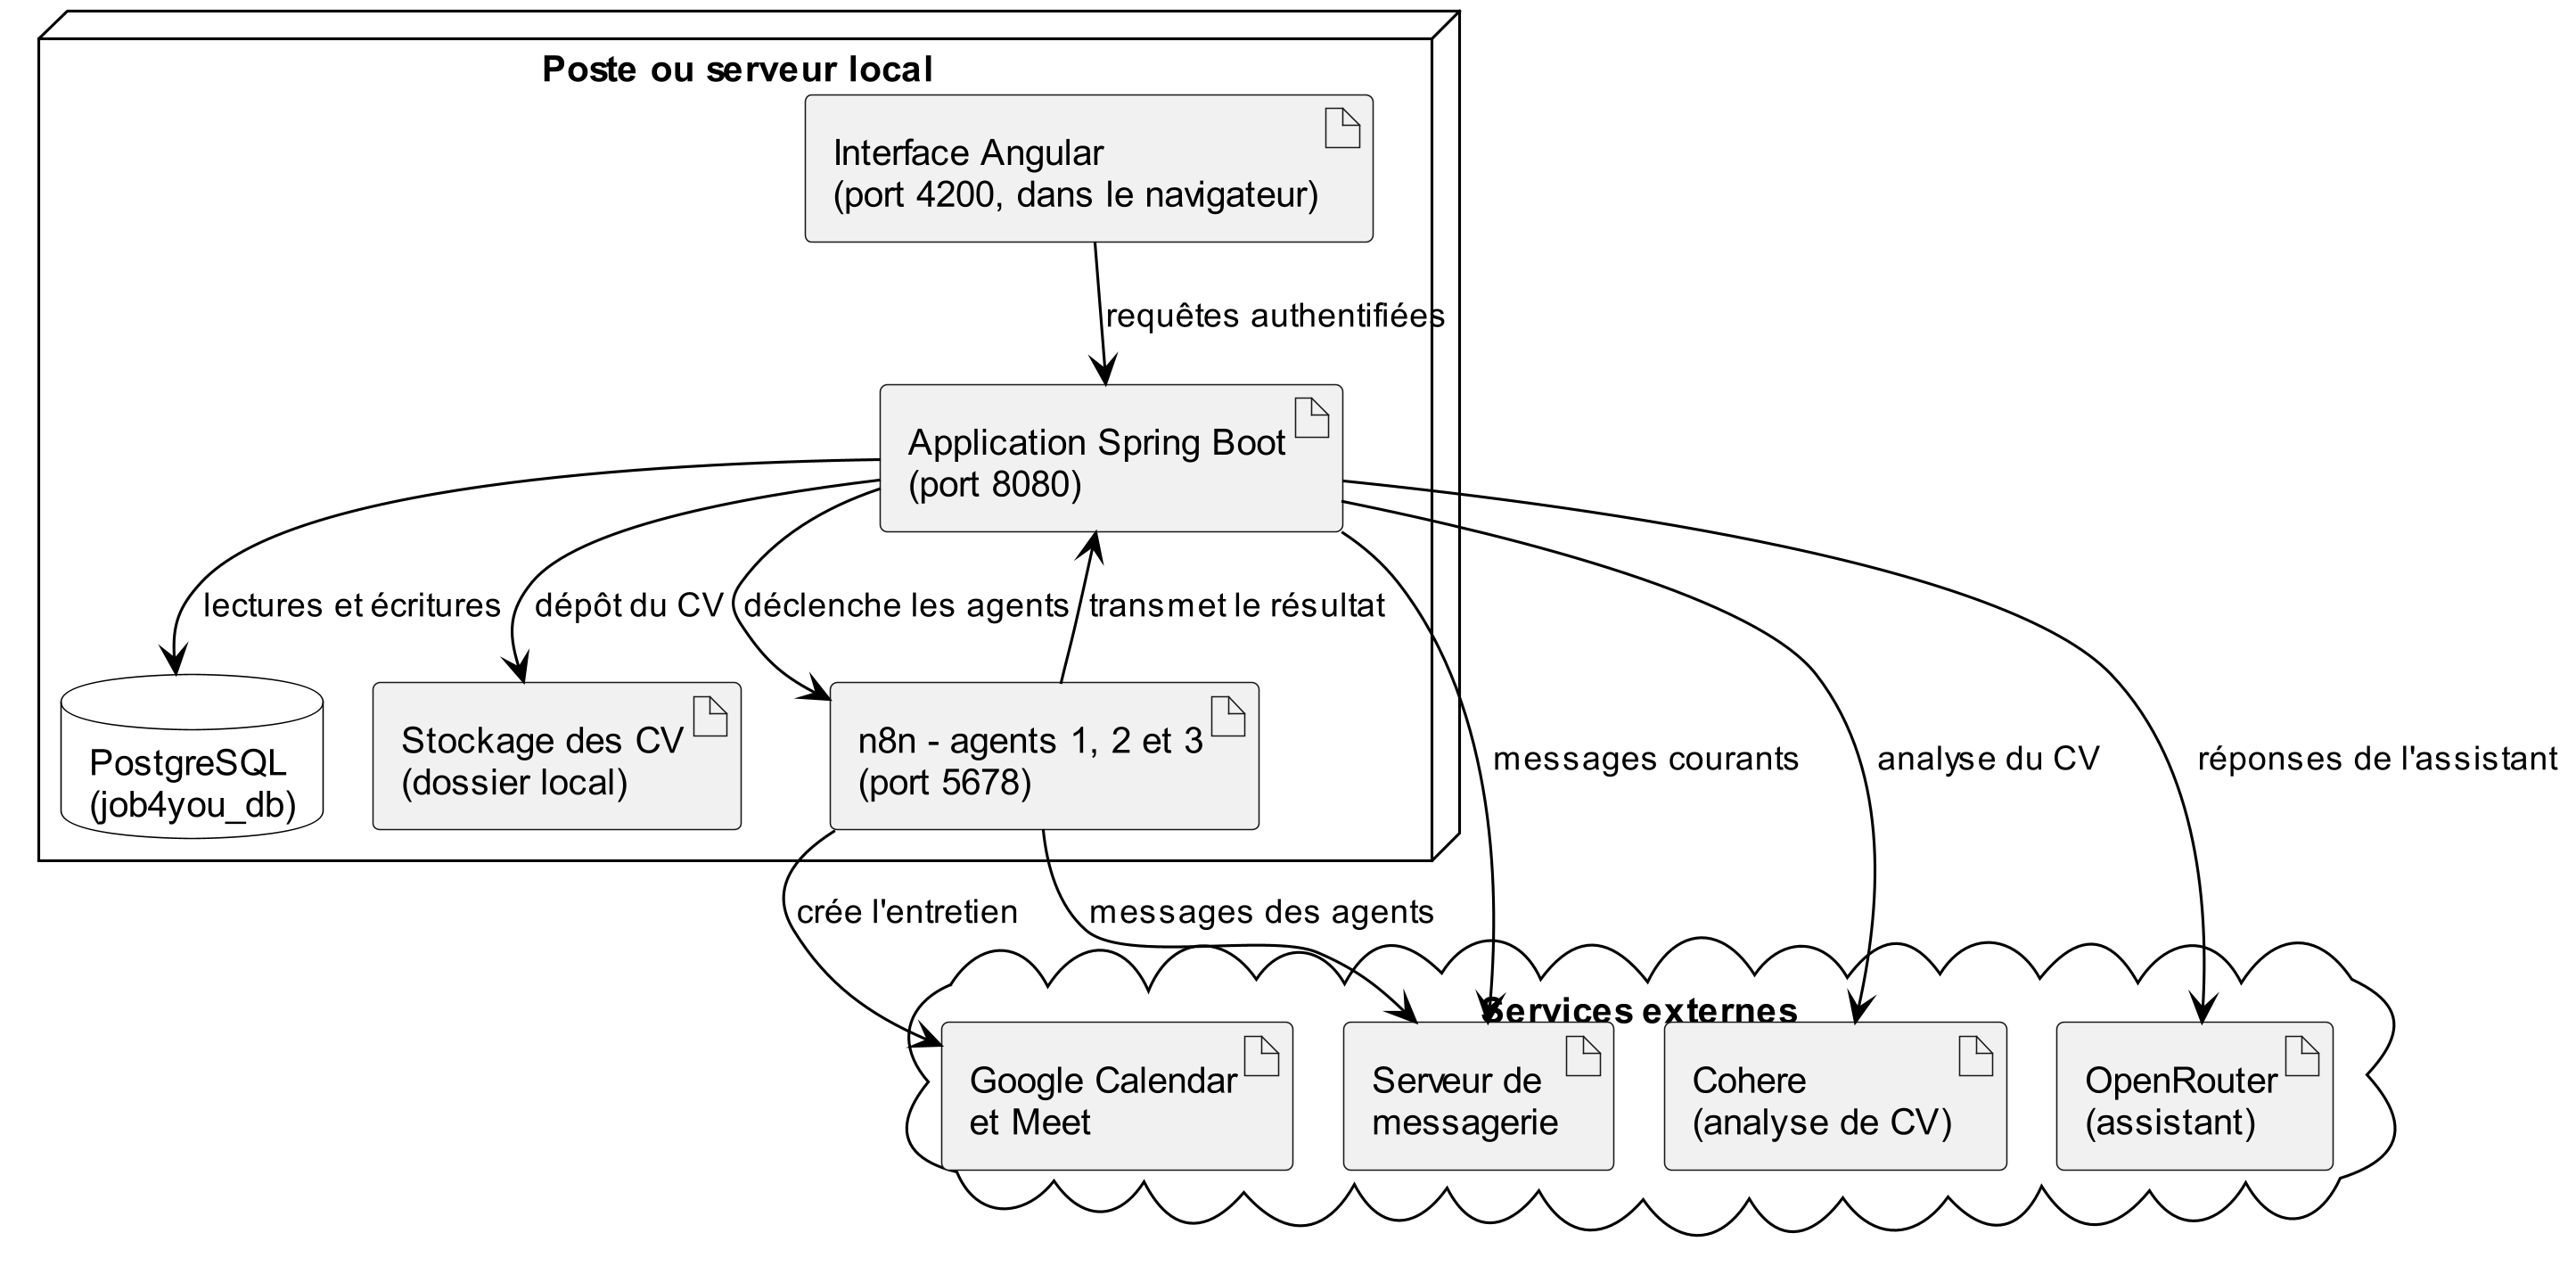
\includegraphics[width=0.98\linewidth, height=0.92\textheight, keepaspectratio]{fig3_11}
\caption{Diagramme de déploiement de la plateforme JOB4YOU}
\label{fig_3_11}
\end{figure}
\clearpage
\end{landscape}

En configuration de développement, Angular, Spring Boot, les agents n8n et le stockage des CV tiennent sur un même poste, PostgreSQL assurant la persistance. Le navigateur parle au back-end par API REST protégées par JWT ; le back-end déclenche n8n par webhooks HTTP et appelle Cohere pour le scoring, OpenRouter pour l’assistant.

\section{Conclusion}
\label{sec_3_10}
Ces modèles (paquetages, classes, séquences, états, base de données, déploiement et composants) forment ensemble le plan directeur qui a guidé le développement de l’application, avec les ajustements décrits au chapitre suivant. Reste à voir comment ce plan s’est concrètement traduit en une application fonctionnelle : c’est l’objet du chapitre suivant.

        % ======== fin chap_03 ========
        \clearpage
        \jobFixLists{chap04}
        % ======== chap_04 ========
\chapter{Réalisation}

Ce dernier chapitre est celui où la conception prend enfin forme concrète. J’y présente l’environnement de travail utilisé, les interfaces réellement développées et fonctionnelles, la démarche de test suivie, ainsi que certaines difficultés rencontrées en cours de route et la façon dont je les ai résolues.

\section{Introduction}
\label{sec_4_1}
Toutes les captures d’écran qui suivent proviennent de l’application en fonctionnement, pas de maquettes : chaque interface présentée a été testée et utilisée pendant le stage.

\section{Environnement de travail}
\label{sec_4_2}
\subsection{Environnement matériel}
\label{sec_4_2_1}
J’ai réalisé le développement sur un poste de travail standard fourni par l’entreprise. Son processeur multi-cœurs et sa mémoire vive exécutent en parallèle l’environnement de développement, les serveurs back-end et front-end, PostgreSQL et n8n en local.

\subsection{Environnement logiciel}
\label{sec_4_2_2}
Les outils et technologies suivants ont été mobilisés tout au long du projet :

\begin{itemize}
\item Langages : \logo{java} Java 17, TypeScript, HTML5, SCSS, SQL.
\item Frameworks et bibliothèques : \logo{spring} Spring Boot 3 (Web, Data JPA, Security), \logo{angular} Angular 20, \logo{bootstrap} Bootstrap.
\item Base de données : \logo{postgres} PostgreSQL, administrée via pgAdmin.
\item Automatisation et IA : \logo{n8n} n8n (agents d’automatisation par webhooks), API de Cohere (scoring IA des CV). Assistant conversationnel candidat : API OpenRouter (modèle z-ai/glm-5.3-flash, format compatible OpenAI).
\item Environnements intégrés : Eclipse STS (Spring Tool Suite) pour le back-end Java/Spring Boot, Visual Studio Code pour le front-end Angular.
\item Modélisation UML : StarUML pour la conception des diagrammes de cas d’utilisation, de classes et de séquence présentés aux chapitres 2 et 3 ; le rendu graphique des figures a été produit avec PlantUML à partir de la description textuelle de ces modèles.
\item Gestion de version : \logo{git} Git, hébergement du code sur GitHub.
\item Outils de test et de documentation d’API : Postman pour les tests manuels des API REST, Swagger (springdoc-openapi) pour la documentation interactive générée automatiquement.
\item Build et gestion de dépendances : Maven pour le back-end, npm pour le front-end.
\end{itemize}

\subsection{Gestion de version}
\label{sec_4_2_3}
J’ai organisé le versionnement du code autour d’une branche principale, avec des messages de commit descriptifs qui facilitent la traçabilité des évolutions fonctionnelles et des corrections apportées tout au long du stage.

\subsection{Sécurité applicative}
\label{sec_4_2_4}
Plusieurs mécanismes concrets protègent la plateforme et les données des candidats. Les mots de passe ne sont jamais stockés en clair : ils sont hachés avec BCrypt avant persistance.

\begin{itemize}
\item \textbf{Authentification} : un jeton JWT signé \cite{ref14}, valable 24 heures, transmis à chaque requête et vérifié côté back-end, qui en extrait l’identité et les rôles de l’utilisateur.
\item \textbf{Autorisation} : chaque point d’entrée de l’API REST est protégé par annotation selon le rôle requis (\texttt{@PreAuthorize}). Un contrôle supplémentaire restreint, pour un manager, la visibilité aux seuls candidats de son périmètre — déterminé prioritairement par son département, la famille de métier ne servant de repli que pour les offres non rattachées à un département.
\item \textbf{Téléversement} : le dépôt de CV est limité aux formats PDF, DOC et DOCX, avec une taille maximale de 10 Mo côté API, resserrée à 5 Mo par la validation du formulaire Angular.
\end{itemize}

Reste, avant une mise en production, à ajouter une analyse antivirus et une validation du contenu plus poussée que la seule extension et le type MIME, conformément aux recommandations de l’OWASP \cite{ref15}.

\section{Interfaces graphiques de l’application}
\label{sec_4_3}
Les captures sont regroupées par acteur : l’accès public et l’espace candidat (figures~\ref{fig_4_1} à \ref{fig_4_5}), le suivi RH du recrutement (figures~\ref{fig_4_6} à \ref{fig_4_14}). Viennent ensuite l’espace manager (figures~\ref{fig_4_15a}, \ref{fig_4_15b}, \ref{fig_4_16}, \ref{fig_4_16b} et \ref{fig_4_16c}), l’administration et la traçabilité (figures~\ref{fig_4_17} à \ref{fig_4_19}), puis la chaîne n8n (figures~\ref{fig_4_20} à \ref{fig_4_22}). Chacune provient de l’application en fonctionnement, sans maquette ni image de synthèse.

Les captures pleine page sont présentées en paysage : à contenu identique, leur texte passe d’environ 5,9 pt à 8,5-9,6 pt imprimés après recadrage sur la zone utile (figures~\ref{fig_4_15a}, \ref{fig_4_15b} et \ref{fig_4_17}). Le plancher de lisibilité retenu est de 8,5 pt ; les figures les plus chargées ont été découpées ou recadrées pour ne pas descendre sous ce seuil.

\subsection{Accès public et espace candidat}
\label{sec_4_3_1}
% figure 4.1
\setcounter{figure}{0}
\begin{landscape}
\pagestyle{lscape}
\begin{figure}[p]
\centering
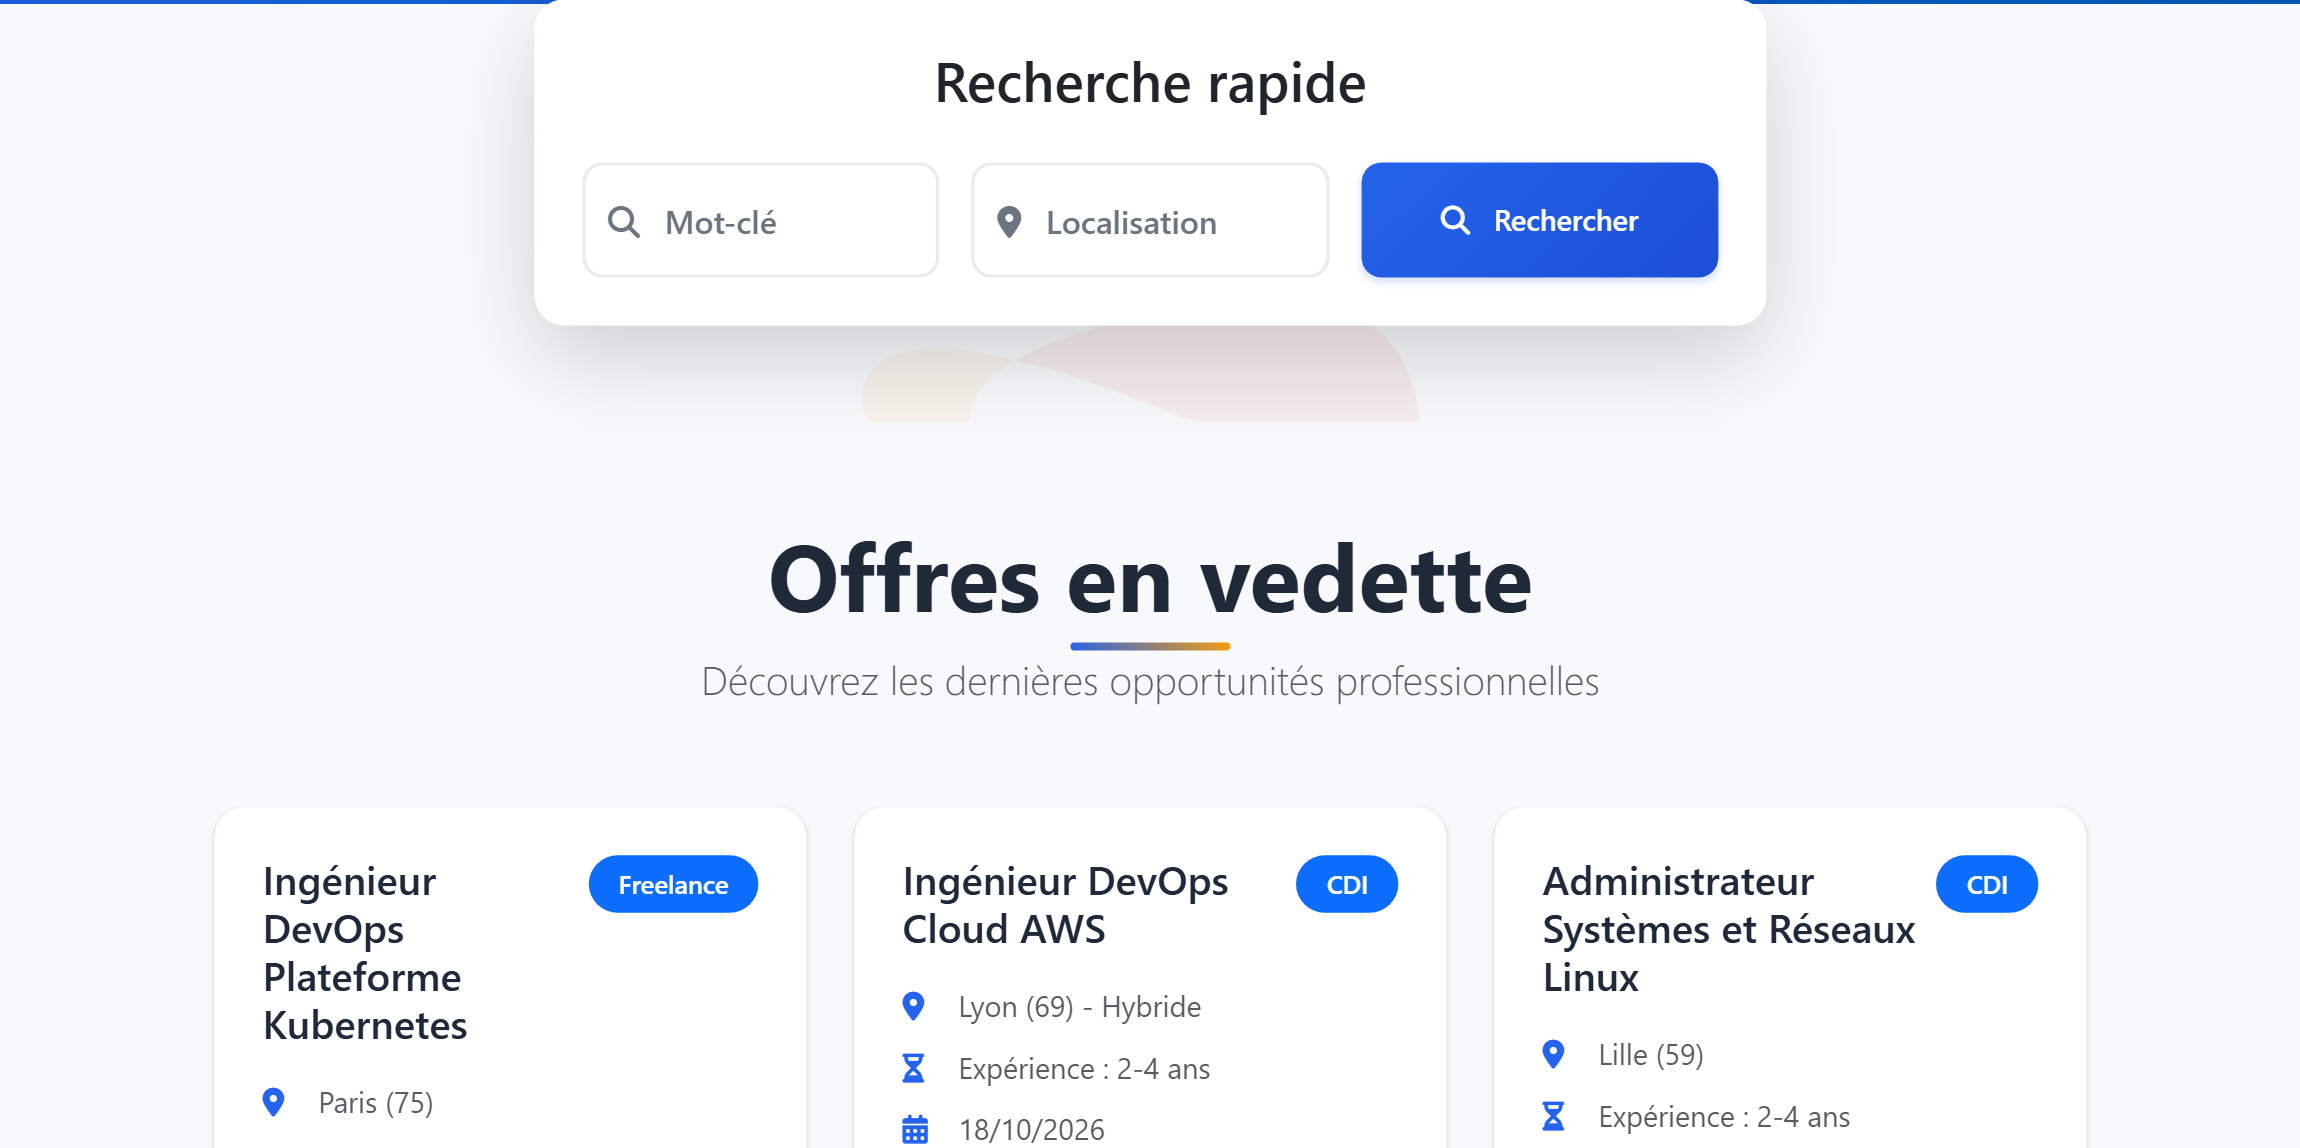
\includegraphics[width=0.98\linewidth, height=0.90\textheight, keepaspectratio]{fig4_1}
\caption{Page d’accueil publique — recherche d’offres d’emploi}
\label{fig_4_1}
\end{figure}
\clearpage
\end{landscape}

Accessible sans authentification, la page d’accueil de la figure~\ref{fig_4_1} propose un cartouche de « Recherche rapide » par mot-clé et par localisation. Elle affiche aussi les offres les plus récemment publiées sous le titre « Offres en vedette ». Chaque carte porte l’intitulé du poste, le contrat, le lieu, l’expérience demandée, les compétences clés, la date et un bouton « Voir les détails ».

% figure 4.2
\setcounter{figure}{1}
\begin{figure}[!ht]
\centering
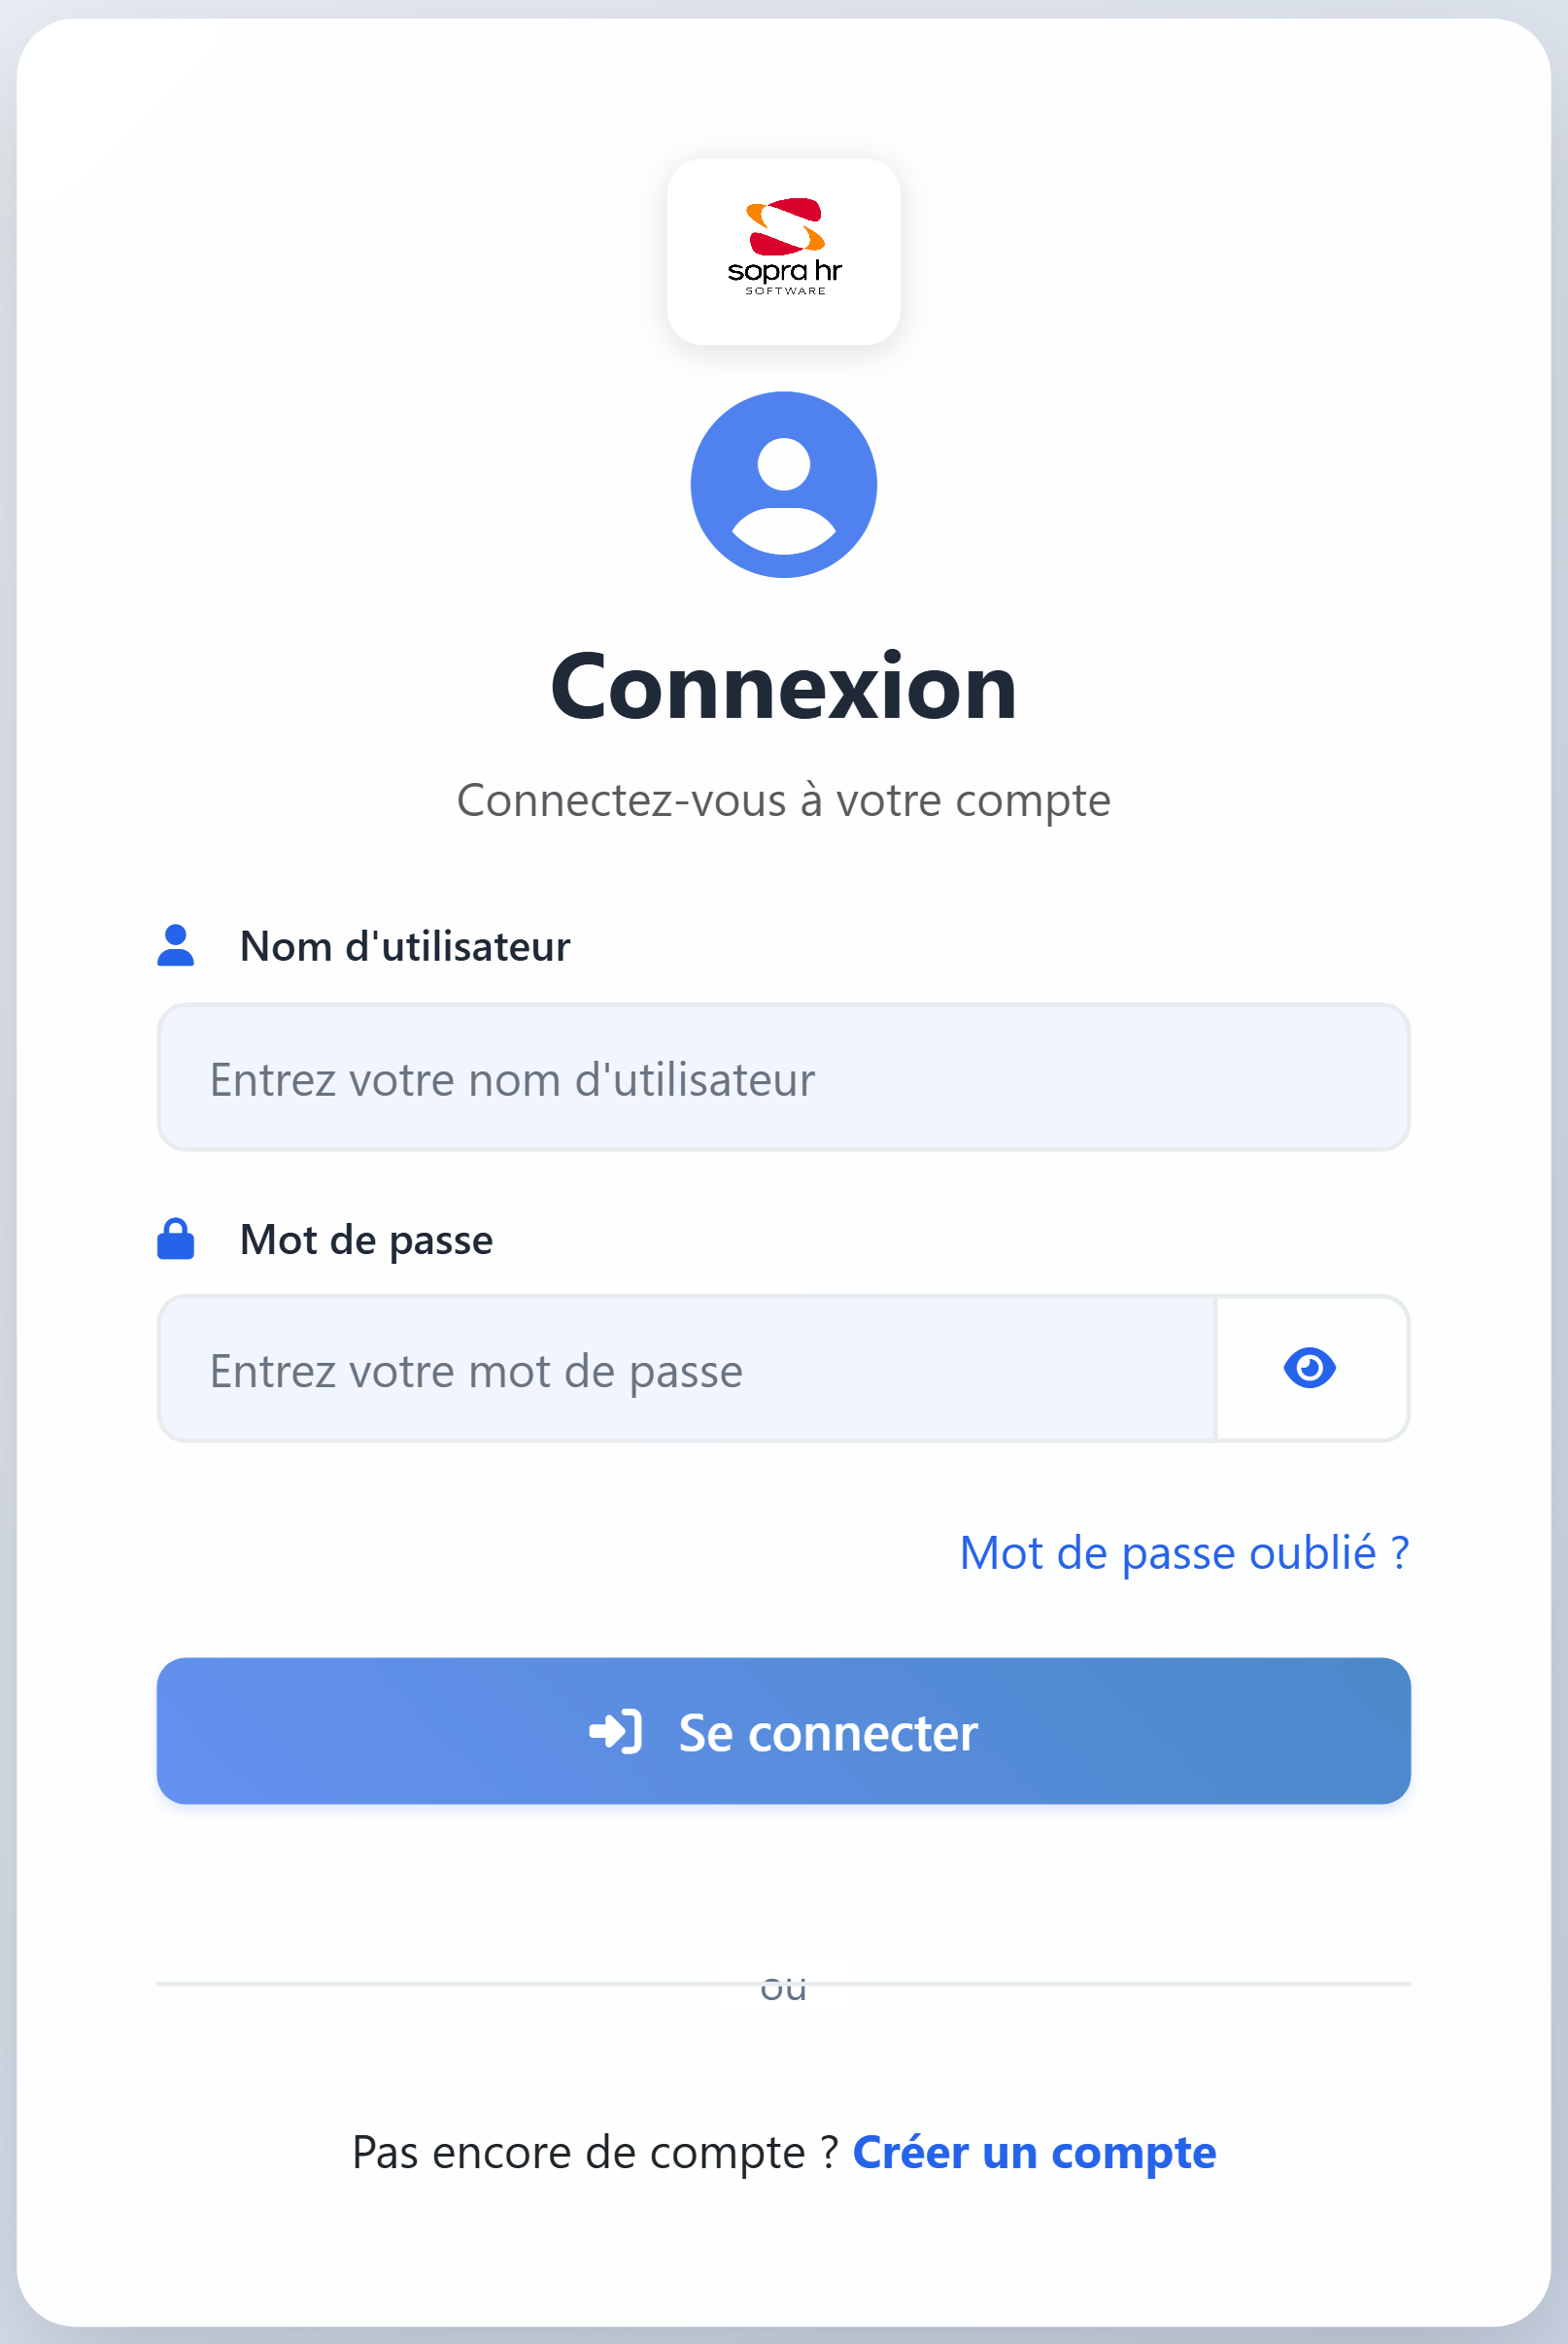
\includegraphics[width=\textwidth, height=0.80\textheight, keepaspectratio]{fig4_2}
\caption{Page de connexion}
\label{fig_4_2}
\end{figure}

La page de connexion de la figure~\ref{fig_4_2} est le point d’entrée des espaces sécurisés : l’authentification s’y fait par nom d’utilisateur et mot de passe, et le jeton JWT renvoyé par le back-end sécurise ensuite l’ensemble des requêtes vers l’API.

% figure 4.3
\setcounter{figure}{2}
\begin{figure}[!ht]
\centering
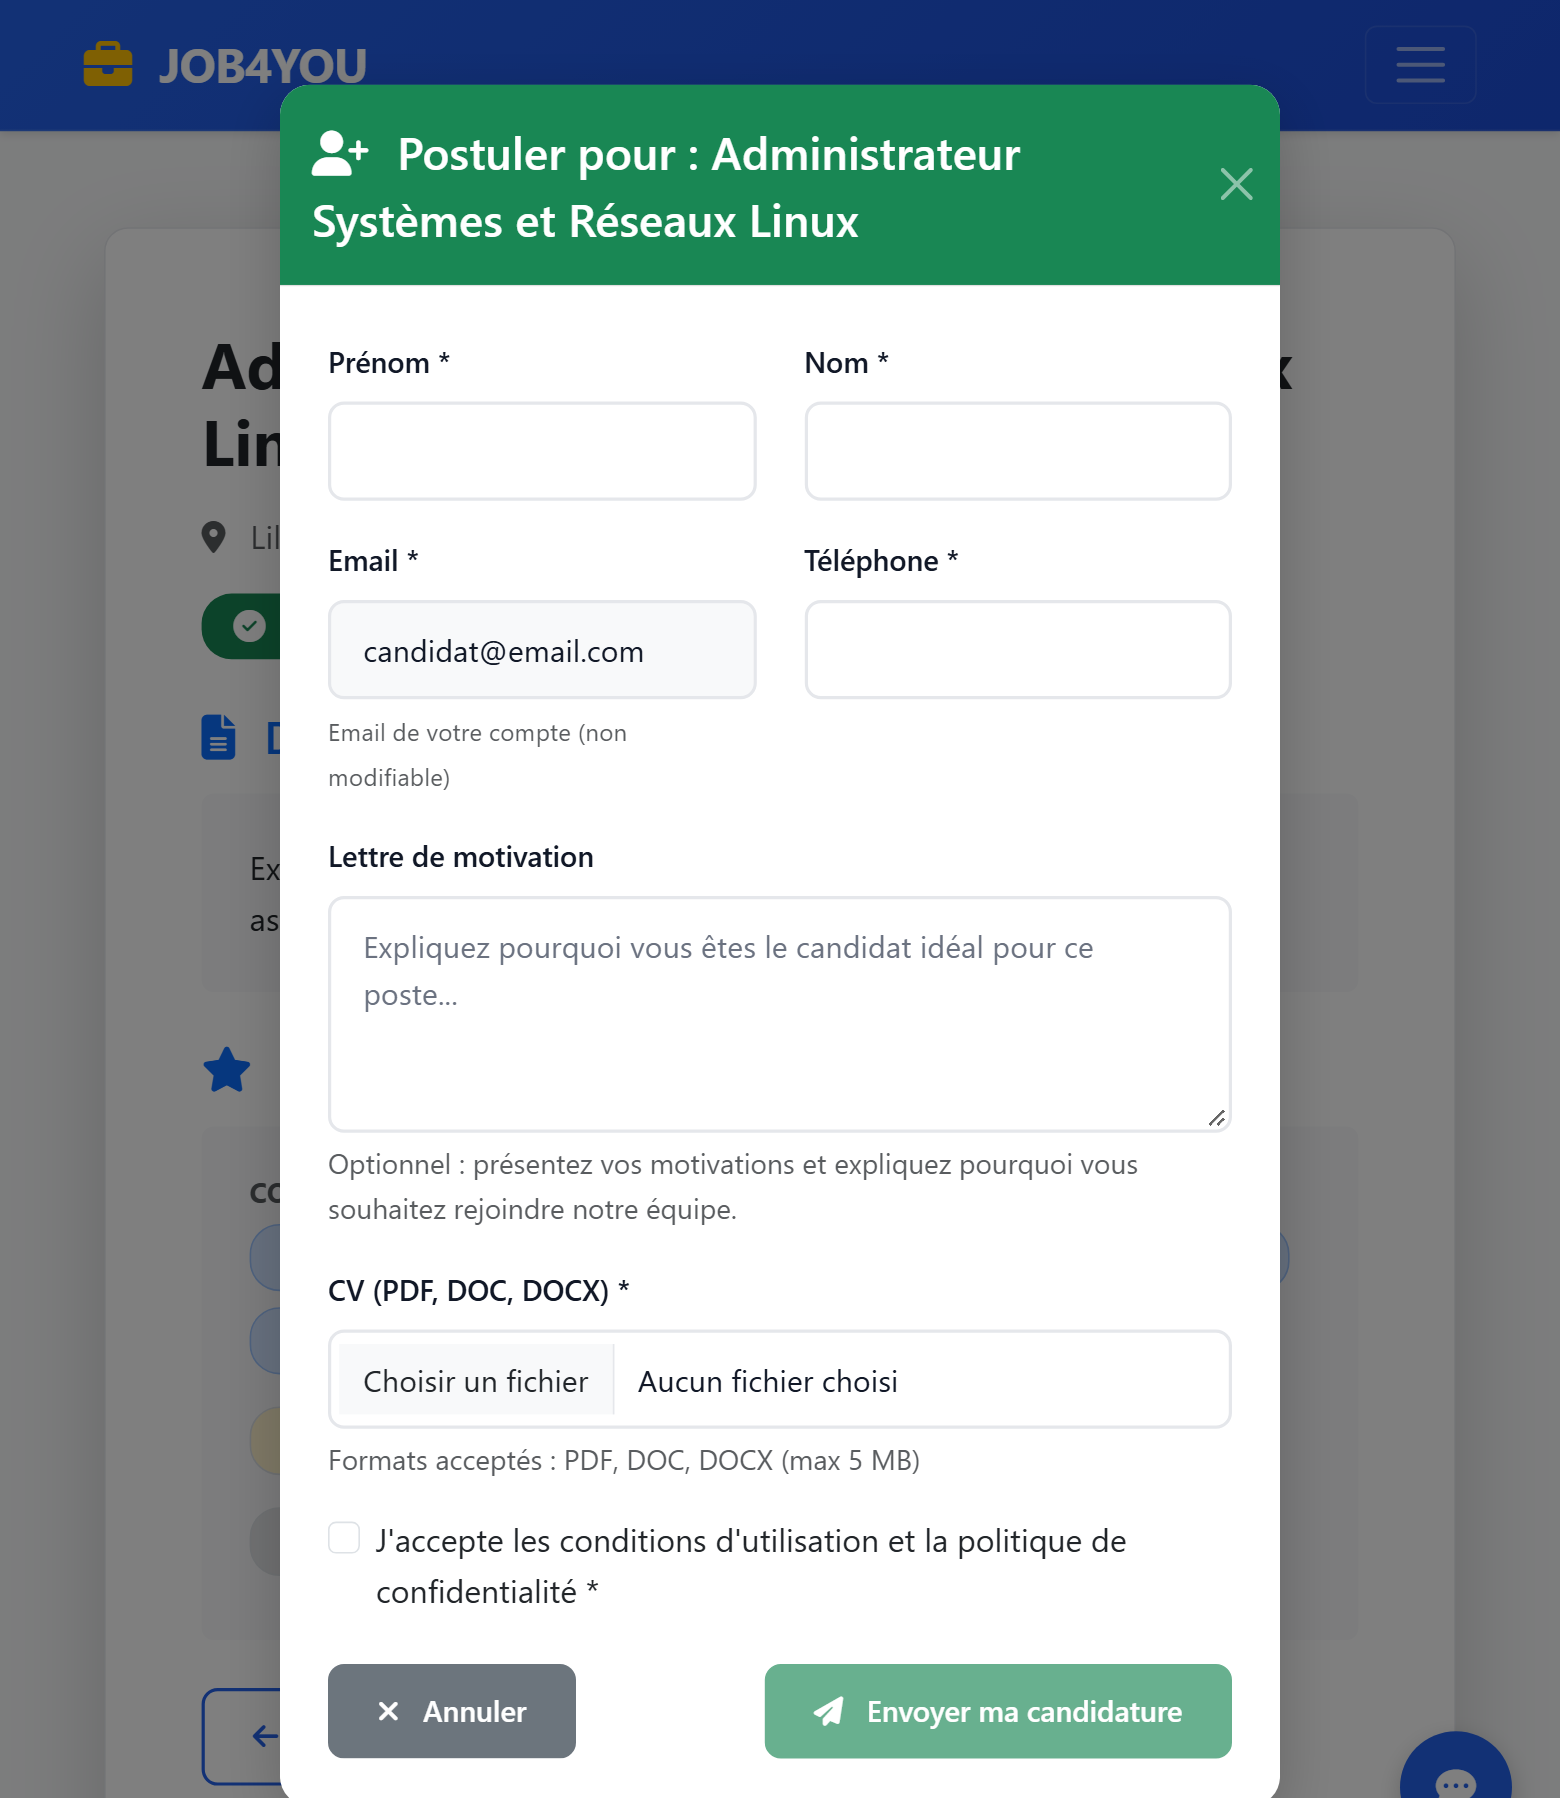
\includegraphics[width=\textwidth, height=0.80\textheight, keepaspectratio]{fig4_3}
\caption{Soumission d’une candidature avec dépôt de CV}
\label{fig_4_3}
\end{figure}

Comme le montre la figure~\ref{fig_4_3}, un candidat connecté postule depuis une offre : le formulaire pré-remplit son e-mail, valide le format du CV (PDF, DOC, DOCX) et confirme la sélection avant l’envoi. Ce dépôt déclenche la chaîne de la section~\ref{sec_3_5_3} (extraction du texte par le back-end, analyse par l’API de Cohere, score automatique).

% figure 4.4
\setcounter{figure}{3}
\begin{landscape}
\pagestyle{lscape}
\begin{figure}[p]
\centering
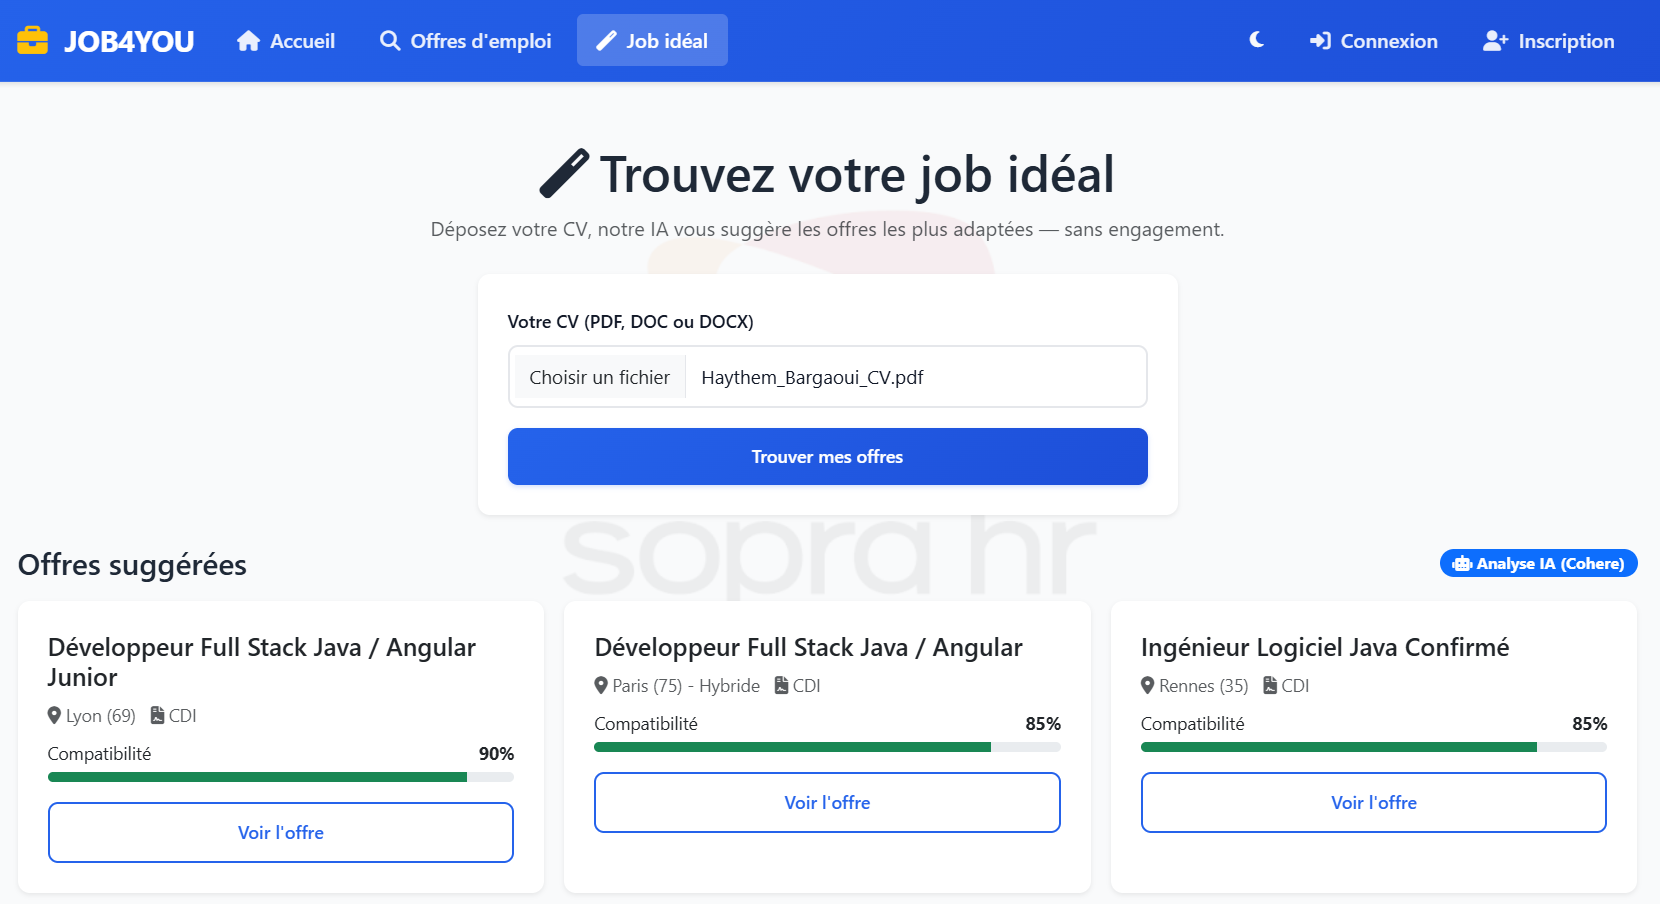
\includegraphics[width=0.98\linewidth, height=0.90\textheight, keepaspectratio]{fig4_4}
\caption{Fonctionnalité « Job idéal » — suggestions d’offres selon le CV}
\label{fig_4_4}
\end{figure}
\clearpage
\end{landscape}

Comme l’illustre la figure~\ref{fig_4_4}, un visiteur qui ne postule à aucune offre précise peut déposer son CV. La plateforme lui renvoie les offres actives classées par pourcentage de compatibilité, calculé par l’API de Cohere et signalé par le badge « Analyse IA (Cohere) ». Si l’IA est indisponible, un repli automatique classe les offres par mots-clés.

% figure 4.5
\setcounter{figure}{4}
\begin{figure}[!ht]
\centering

\includegraphics[width=\textwidth, height=0.80\textheight, keepaspectratio]{fig4_5}
\caption{Assistant conversationnel candidat (chatbot)}
\label{fig_4_5}
\end{figure}

Disponible uniquement pour un candidat authentifié, le widget de la figure~\ref{fig_4_5} permet de poser des questions en langage naturel sur le suivi de ses propres candidatures ou sur le fonctionnement général de la plateforme (offres, Job idéal, retrait de candidature). Les réponses sont générées par un modèle de raisonnement (z-ai/glm-5.3-flash, via l’API OpenRouter).

Le contexte envoyé au modèle est constitué côté serveur par une liste blanche : intitulé du poste, statut, date de candidature, entretiens et retours explicitement transmis au candidat. Les champs internes (score, correction manuelle du RH, identité de l’intervieweur, notes d’entretien) ne quittent jamais le back-end.

Ce filtre structurel, complété par les consignes du message système, a été vérifié sur les scénarios testés, y compris une tentative d’injection de prompt.

\subsection{Espace RH — suivi du processus de recrutement}
\label{sec_4_3_2}
% figure 4.6
\setcounter{figure}{5}
\begin{landscape}
\pagestyle{lscape}
\begin{figure}[p]
\centering
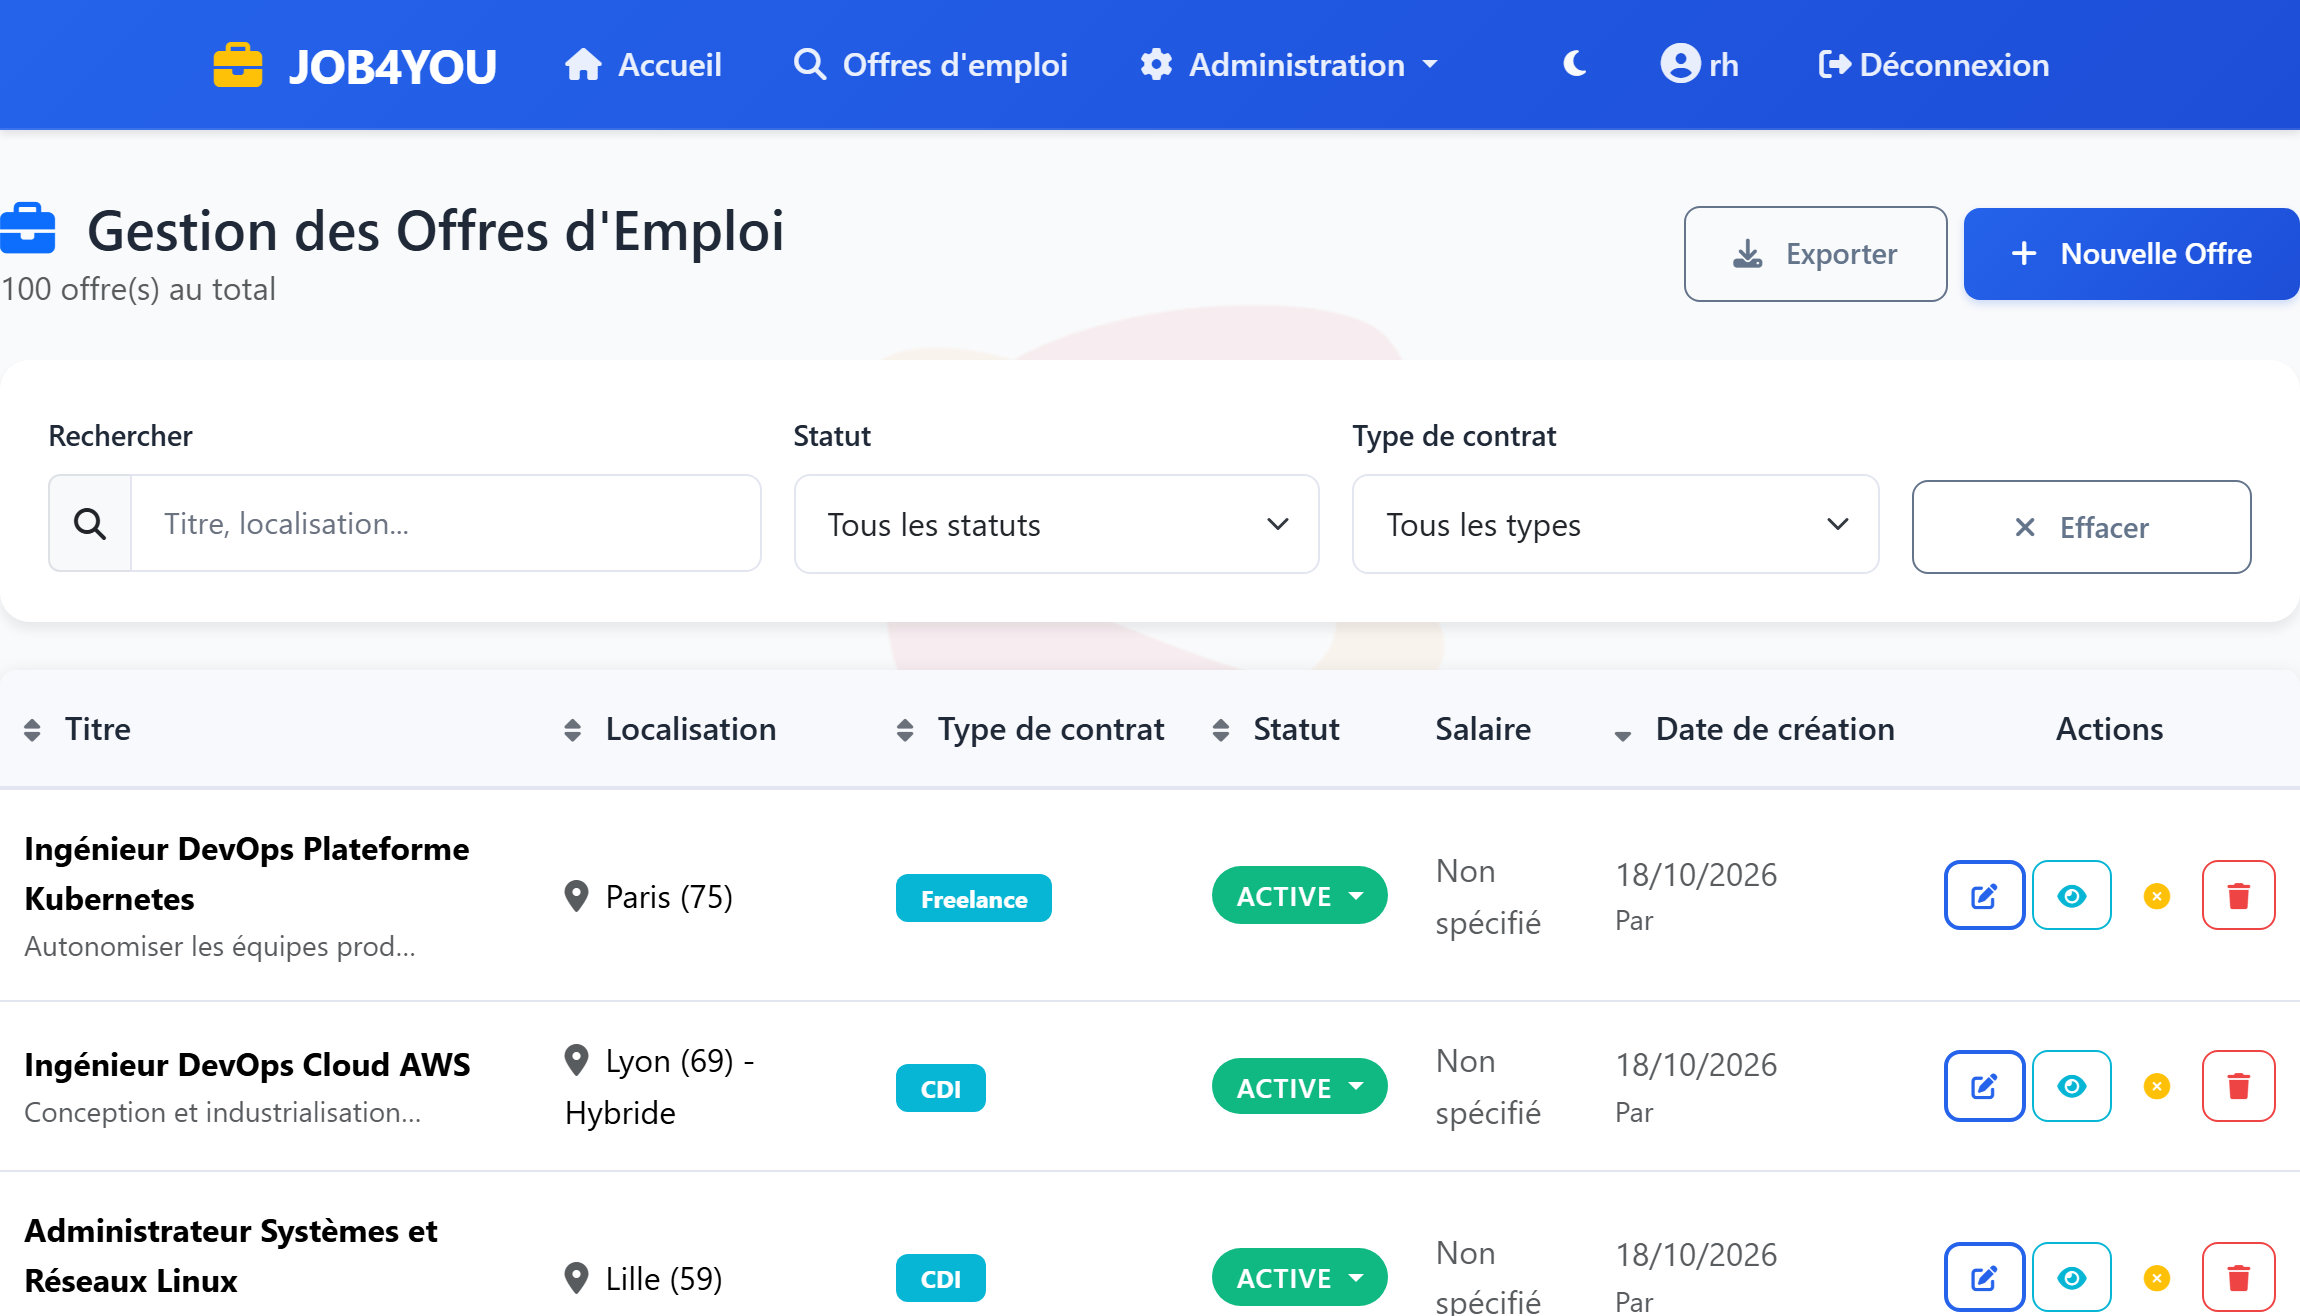
\includegraphics[width=0.98\linewidth, height=0.90\textheight, keepaspectratio]{fig4_6}
\caption{Gestion des offres d’emploi (espace RH)}
\label{fig_4_6}
\end{figure}
\clearpage
\end{landscape}

Comme le montre la figure~\ref{fig_4_6}, le responsable RH crée, modifie et suit le statut de chaque offre depuis une table filtrable par mot-clé, statut et type de contrat. Chaque ligne donne un accès direct à la consultation, la modification et la suppression ; la bascule en « expirée » se fait automatiquement une fois la date limite dépassée.

% figure 4.7
\setcounter{figure}{6}
\begin{landscape}
\pagestyle{lscape}
\begin{figure}[p]
\centering
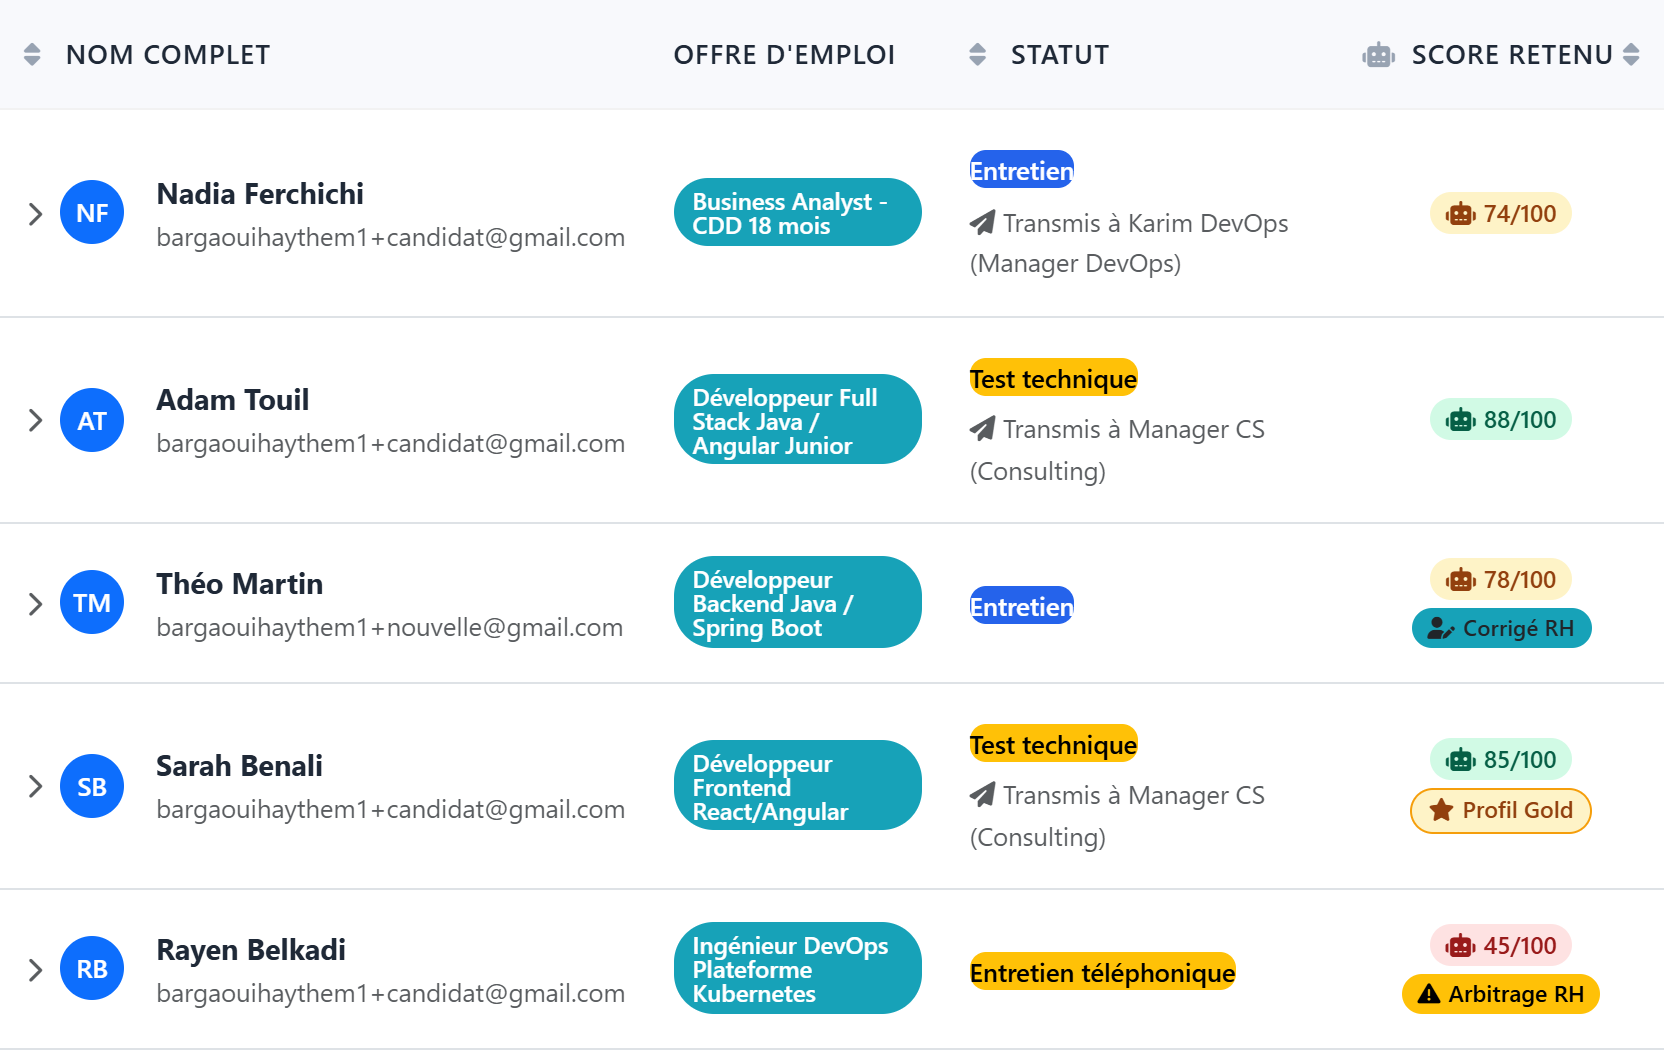
\includegraphics[width=0.98\linewidth, height=0.90\textheight, keepaspectratio]{fig4_7}
\caption{Gestion des candidats — vue liste avec score IA}
\label{fig_4_7}
\end{figure}
\clearpage
\end{landscape}

La figure~\ref{fig_4_7} donne la liste des dossiers de l’espace RH : contact, offre visée, statut courant et score de l’agent IA, coloré selon son niveau. Le bandeau supérieur résume le vivier par quatre compteurs cliquables qui filtrent la liste ; une colonne d’actions rapides ouvre chaque ligne. Ces zones ne sont pas reproduites sur le recadrage.

% figure 4.8
\setcounter{figure}{7}
\begin{figure}[!ht]
\centering
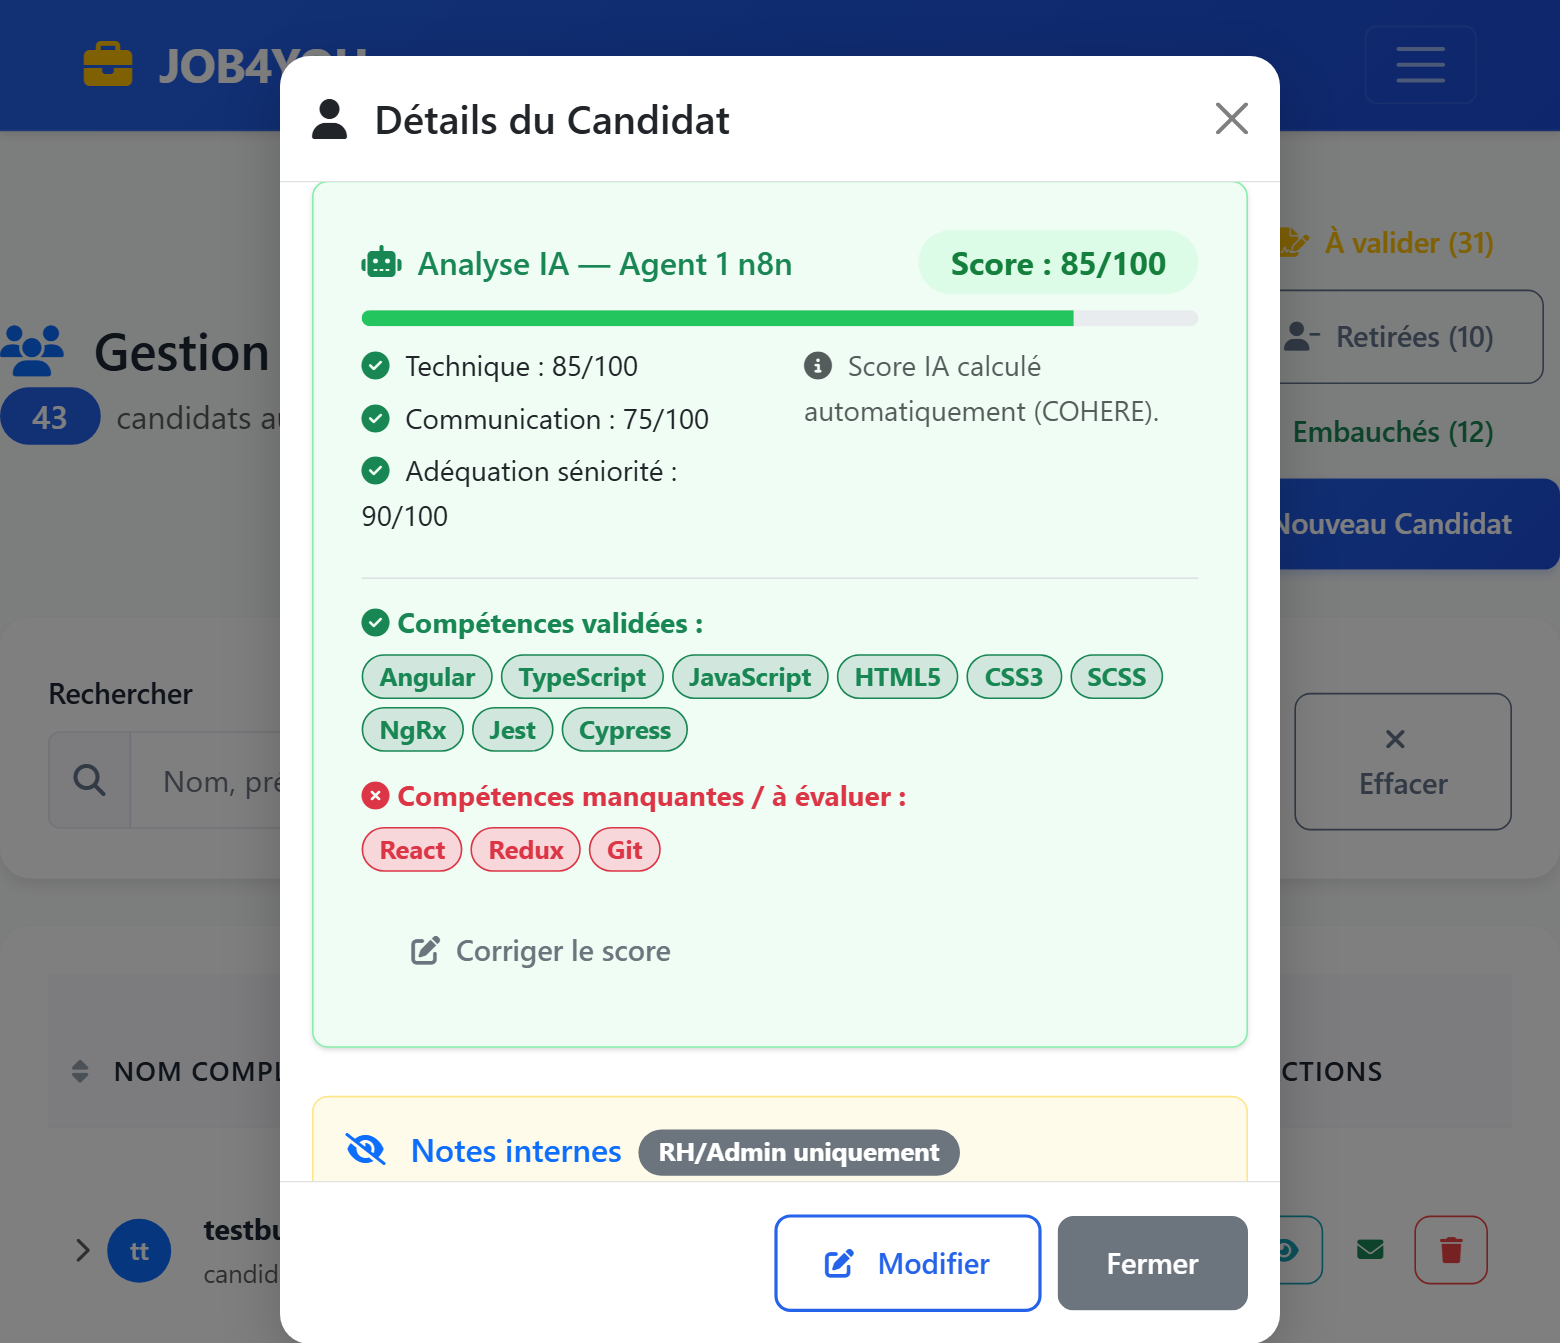
\includegraphics[width=\textwidth, height=0.80\textheight, keepaspectratio]{fig4_8}
\caption{Analyse détaillée d’une candidature par intelligence artificielle}
\label{fig_4_8}
\end{figure}

Le détail d’une candidature, reproduit en figure~\ref{fig_4_8}, va au-delà du score global visible en liste (figure~\ref{fig_4_7}). Il expose la répartition par critère (technique, communication, adéquation séniorité) et le bouton « Corriger le score ». Une correction manuelle du RH s’y affiche avec sa justification, conformément au contrôle humain décrit en section~\ref{sec_4_6}, ainsi que les notes internes et l’activité des agents n8n sur le dossier. S’y ajoute l’étiquette « Profil Gold » : proposée par la machine quand un score atteint la barre d’excellence sur une analyse sûre, elle n’existe pour le manager qu’après confirmation du recruteur (section~\ref{sec_4_4_5}).

% figure 4.9
\setcounter{figure}{8}
\begin{figure}[!ht]
\centering
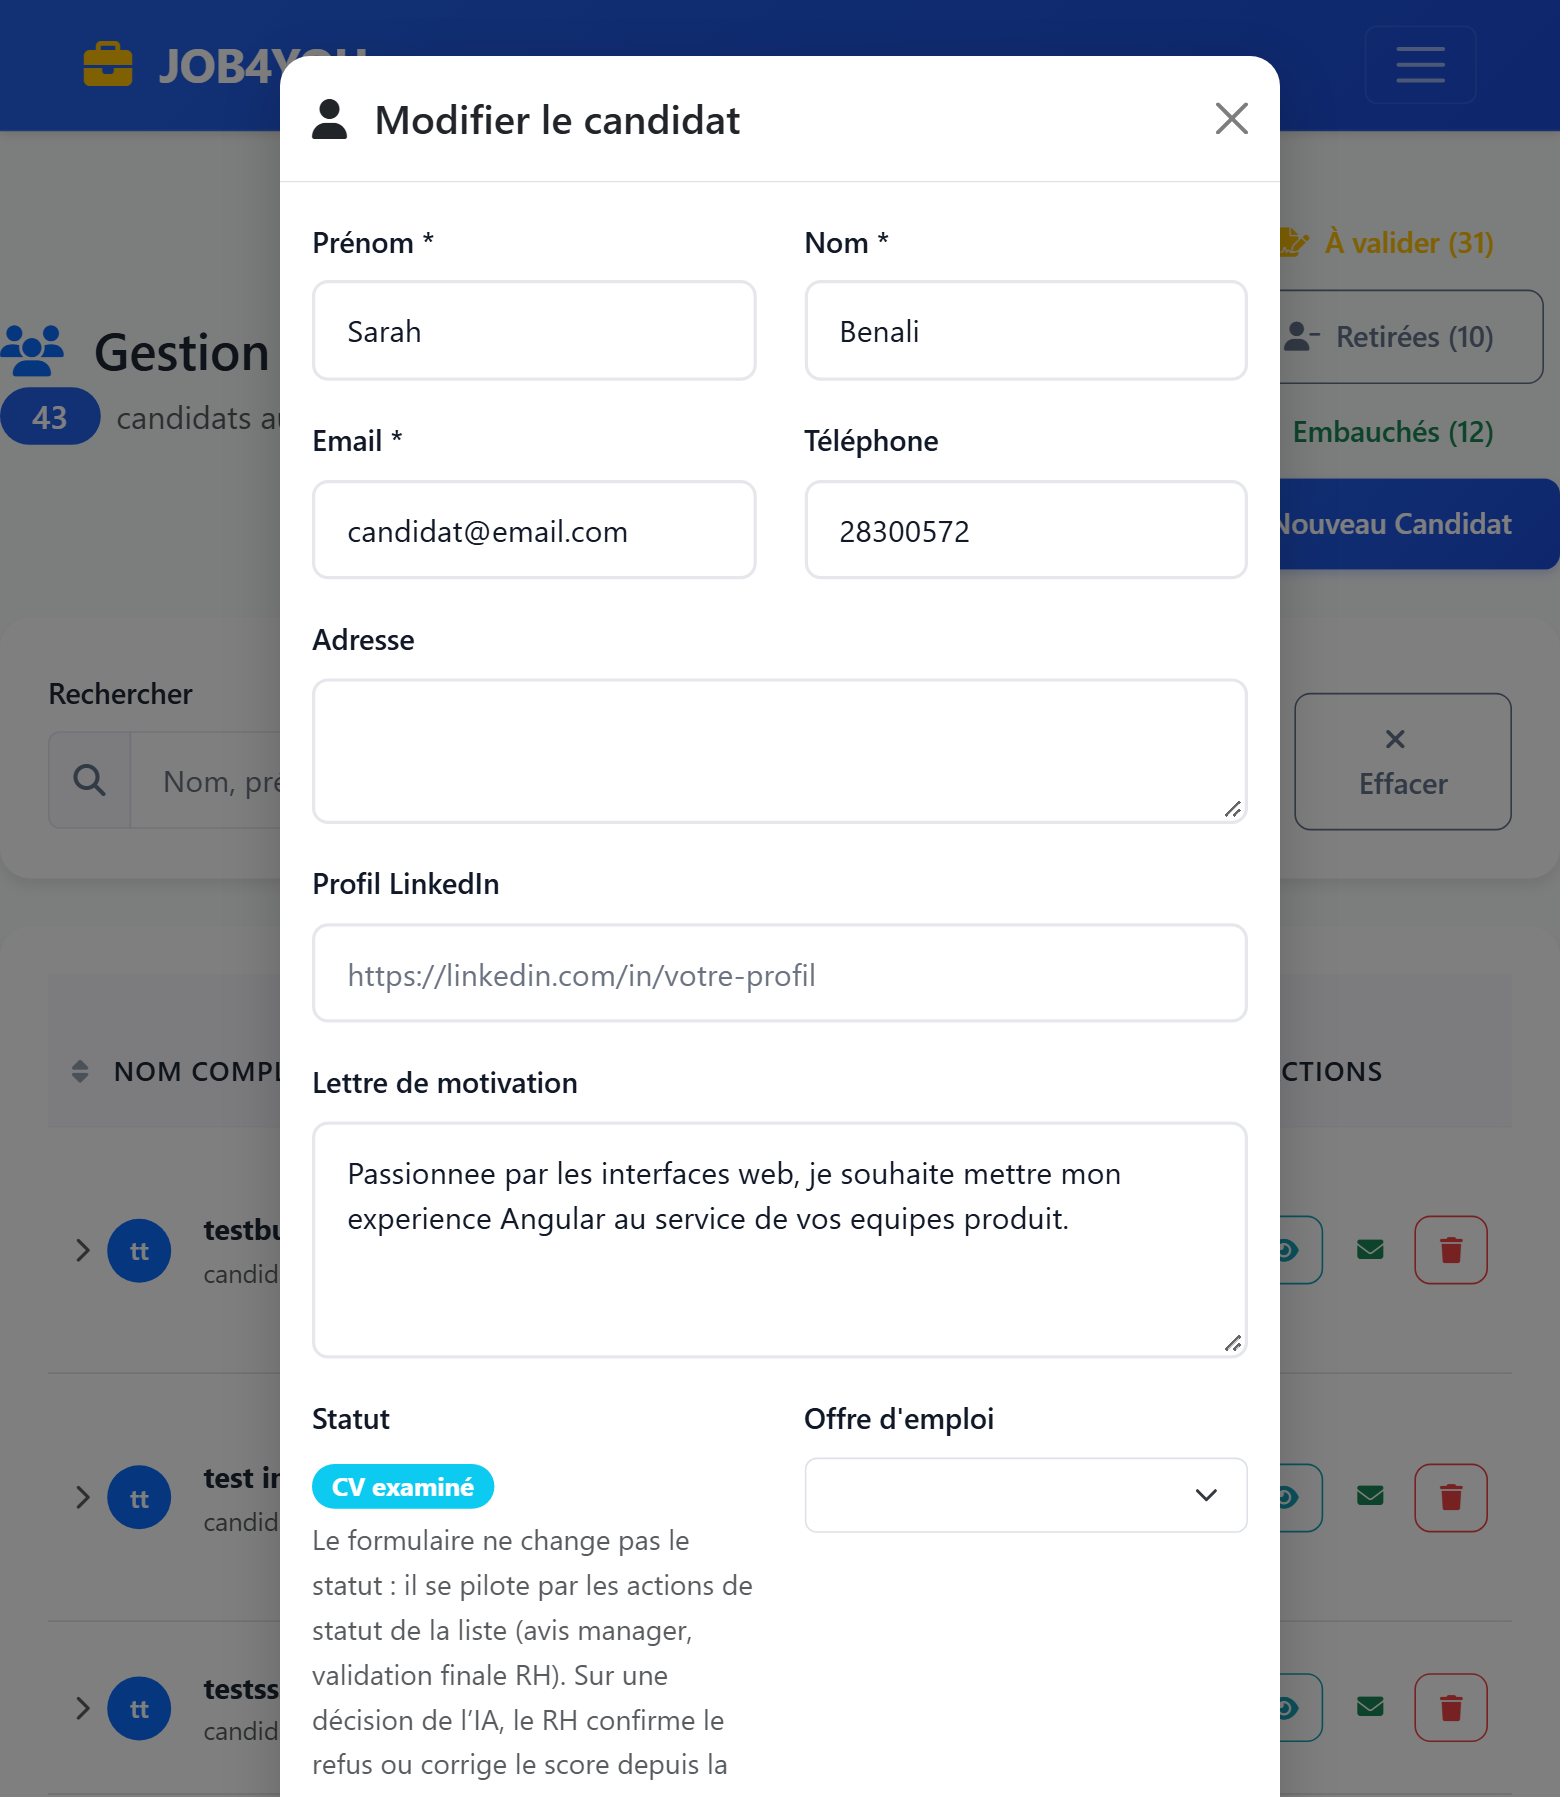
\includegraphics[width=\textwidth, height=0.80\textheight, keepaspectratio]{fig4_9}
\caption{Modification d’un dossier candidat}
\label{fig_4_9}
\end{figure}

Le formulaire de modification (figure~\ref{fig_4_9}) permet de corriger un dossier candidat (coordonnées, lettre, statut, offre associée). La fiche de consultation associée rassemble trois éléments : le CV, lisible en ligne sans téléchargement ; l’analyse IA détaillée (technique, communication, séniorité) ; l’historique des agents n8n pour ce dossier.

% figure 4.10
\setcounter{figure}{9}
\begin{landscape}
\pagestyle{lscape}
\begin{figure}[p]
\centering
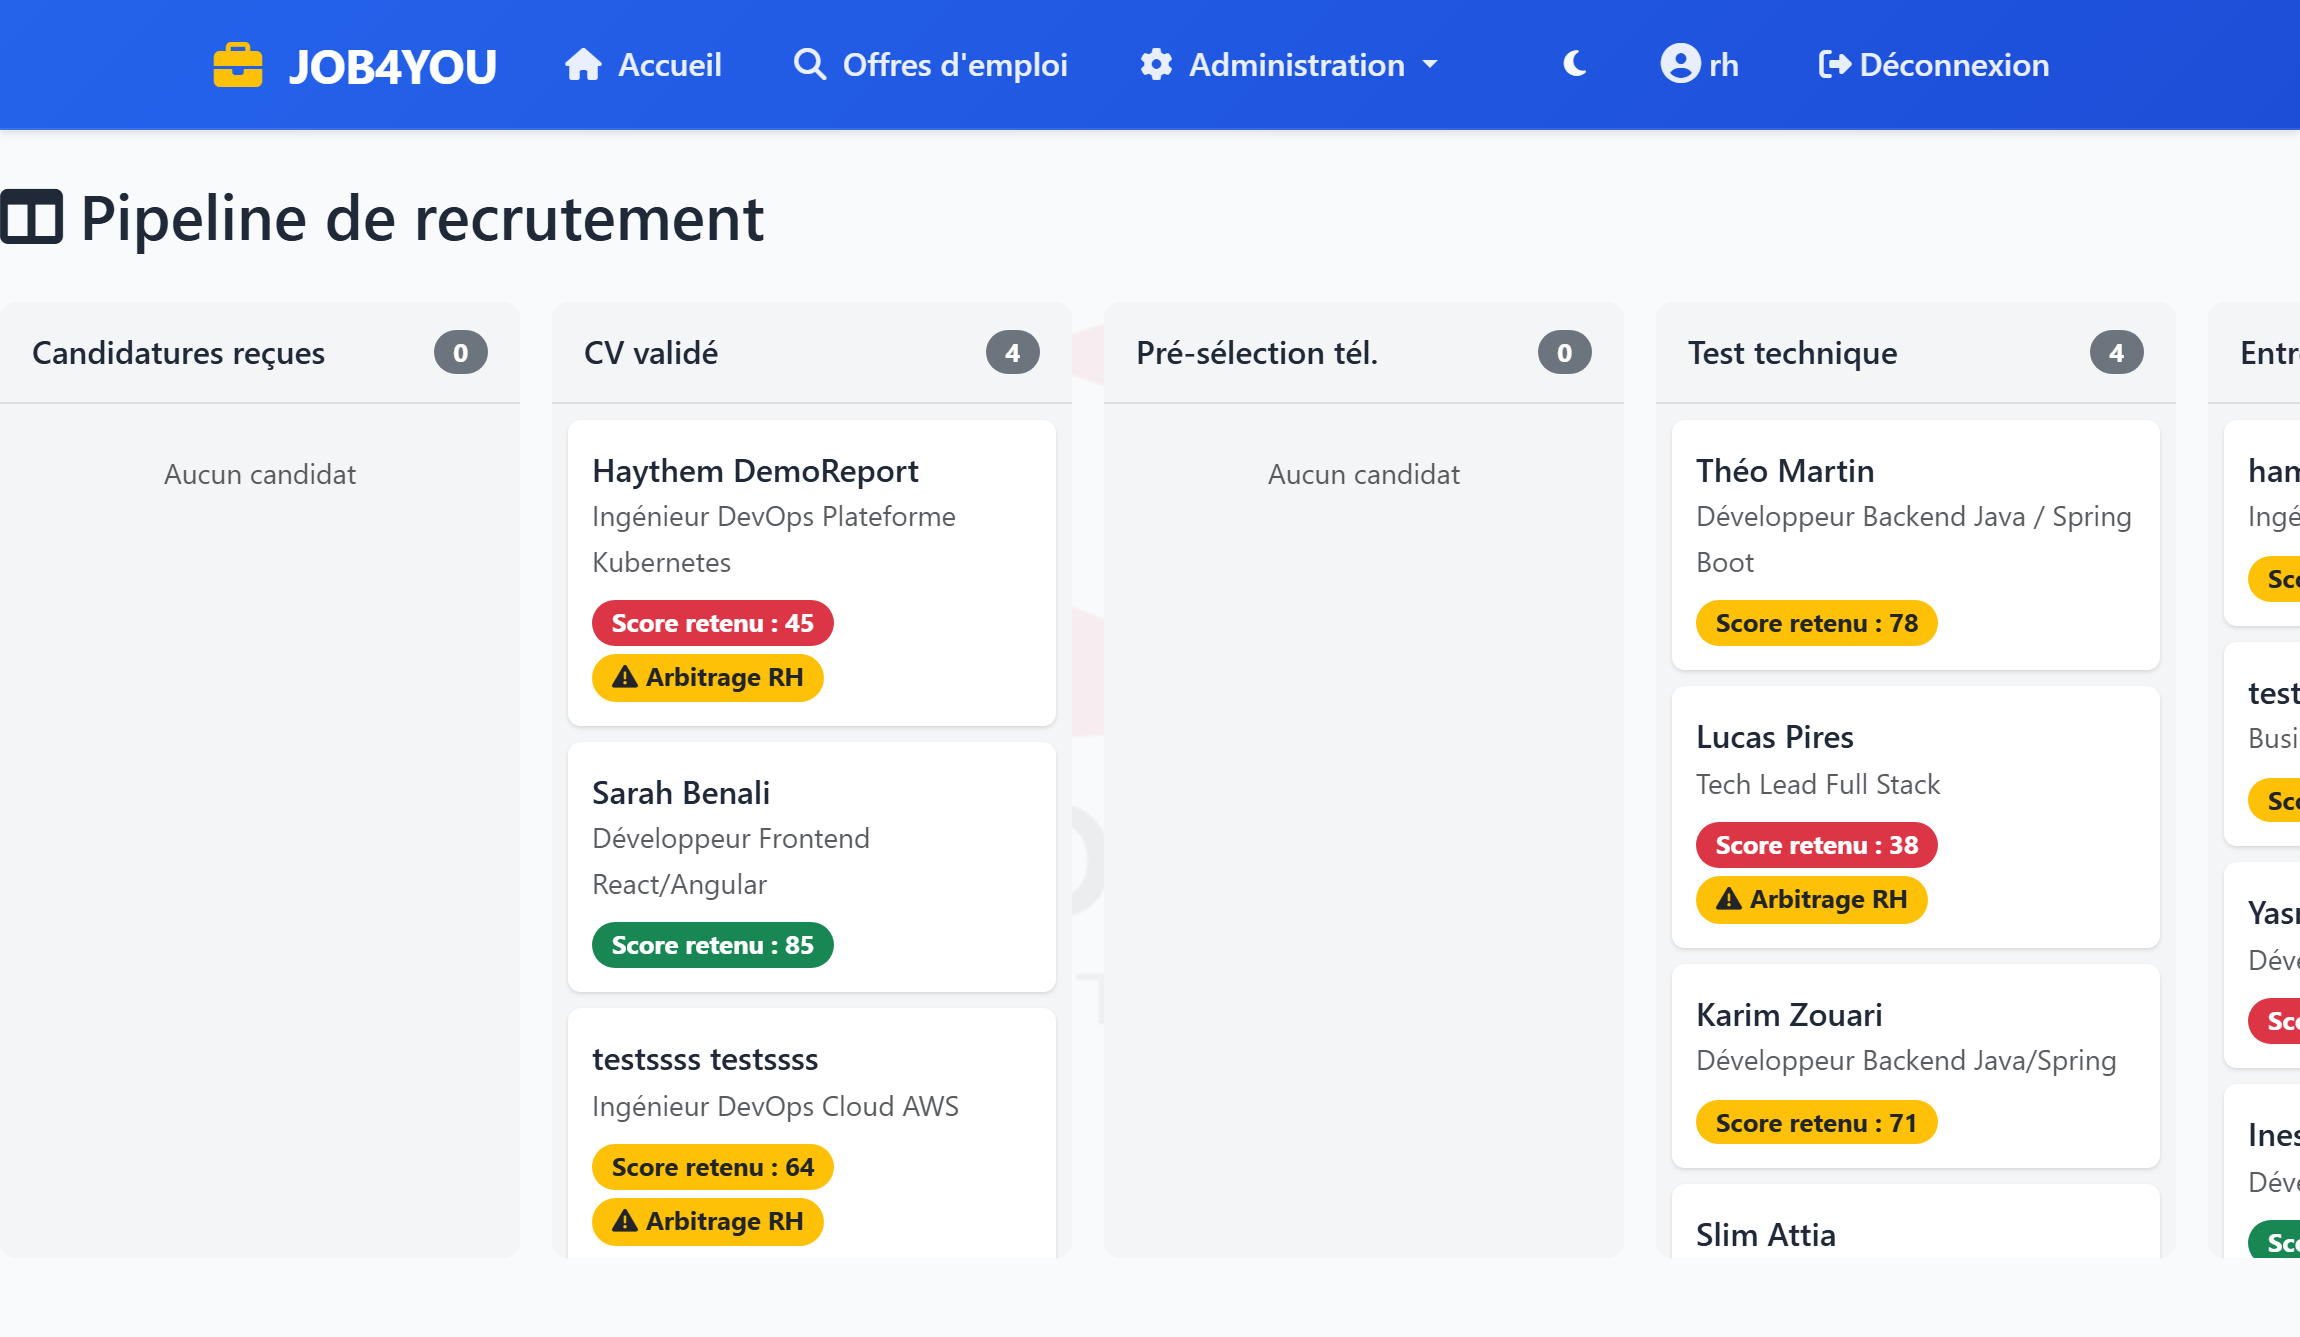
\includegraphics[width=0.98\linewidth, height=0.90\textheight, keepaspectratio]{fig4_10}
\caption{Tableau Kanban du pipeline de recrutement}
\label{fig_4_10}
\end{figure}
\clearpage
\end{landscape}

Le tableau Kanban de la figure~\ref{fig_4_10}, « Pipeline de recrutement », répartit les candidatures par statut : chaque colonne porte son nombre de dossiers, chaque carte le candidat, l’offre visée et le score IA. Les colonnes ne tenant pas à l’écran, le tableau défile horizontalement. Glisser une carte d’une colonne à l’autre met à jour le statut, sous réserve des garde-fous du chapitre 3.

% figure 4.11
\setcounter{figure}{10}
\begin{landscape}
\pagestyle{lscape}
\begin{figure}[p]
\centering
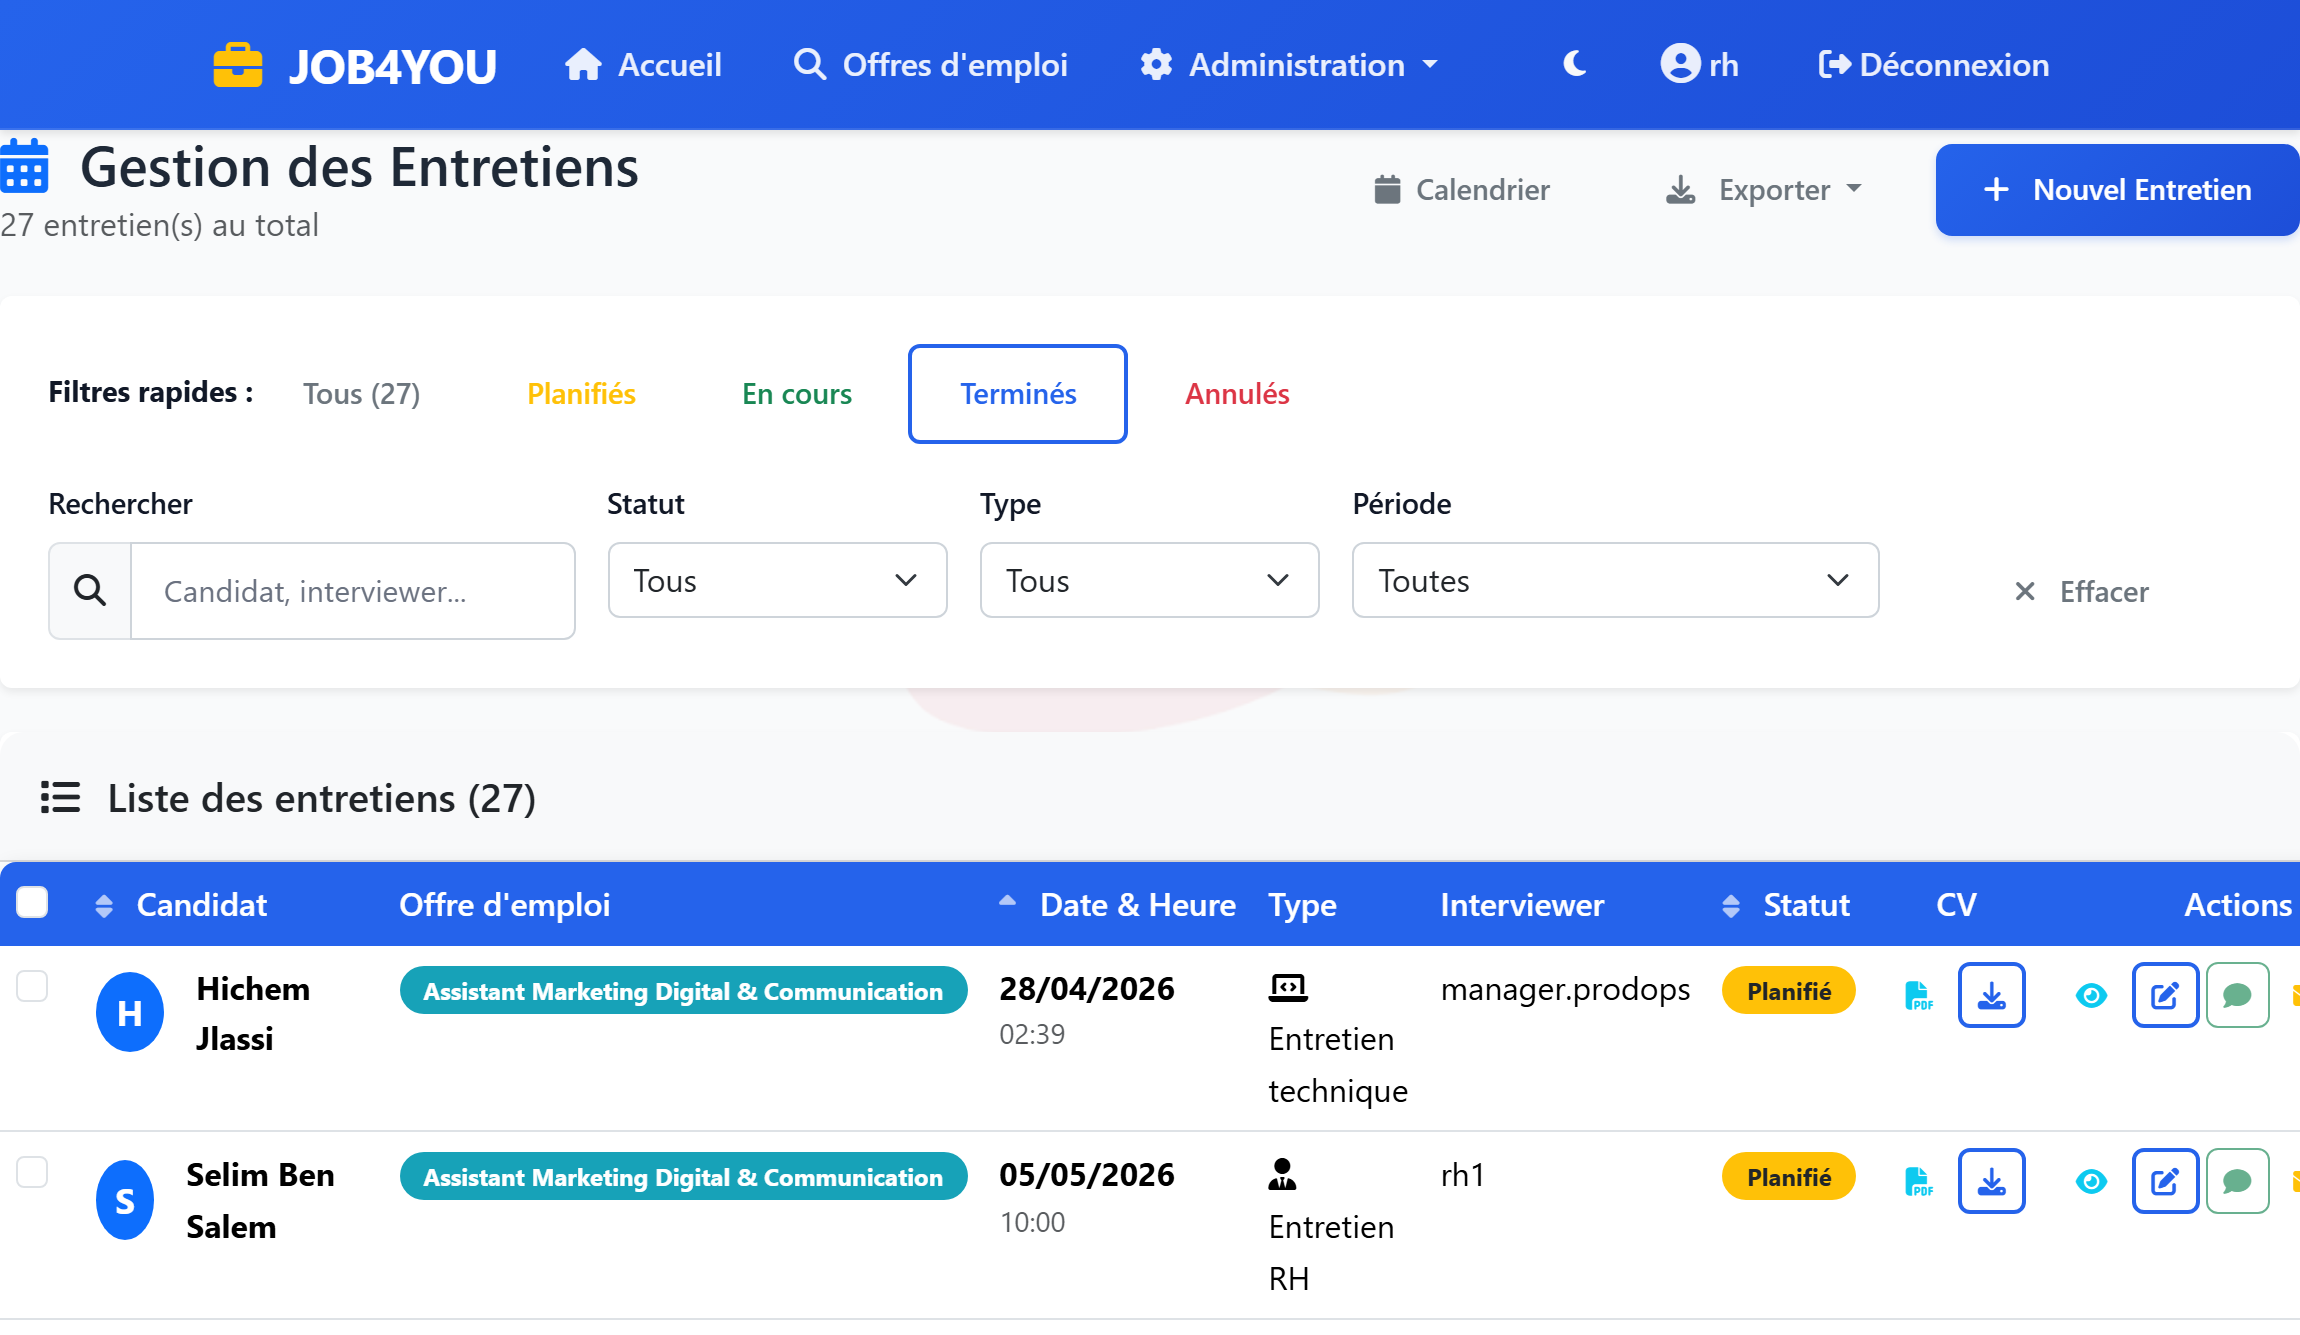
\includegraphics[width=0.98\linewidth, height=0.90\textheight, keepaspectratio]{fig4_11}
\caption{Gestion des entretiens (espace RH)}
\label{fig_4_11}
\end{figure}
\clearpage
\end{landscape}

L’écran de gestion des entretiens de la figure~\ref{fig_4_11} permet de planifier, filtrer et suivre les entretiens par candidat, offre, type, intervieweur et statut. Des actions contextuelles s’ajoutent : démarrer, annuler, reprogrammer ou ajouter un retour une fois l’entretien terminé.

% figure 4.12
\setcounter{figure}{11}
\begin{landscape}
\pagestyle{lscape}
\begin{figure}[p]
\centering
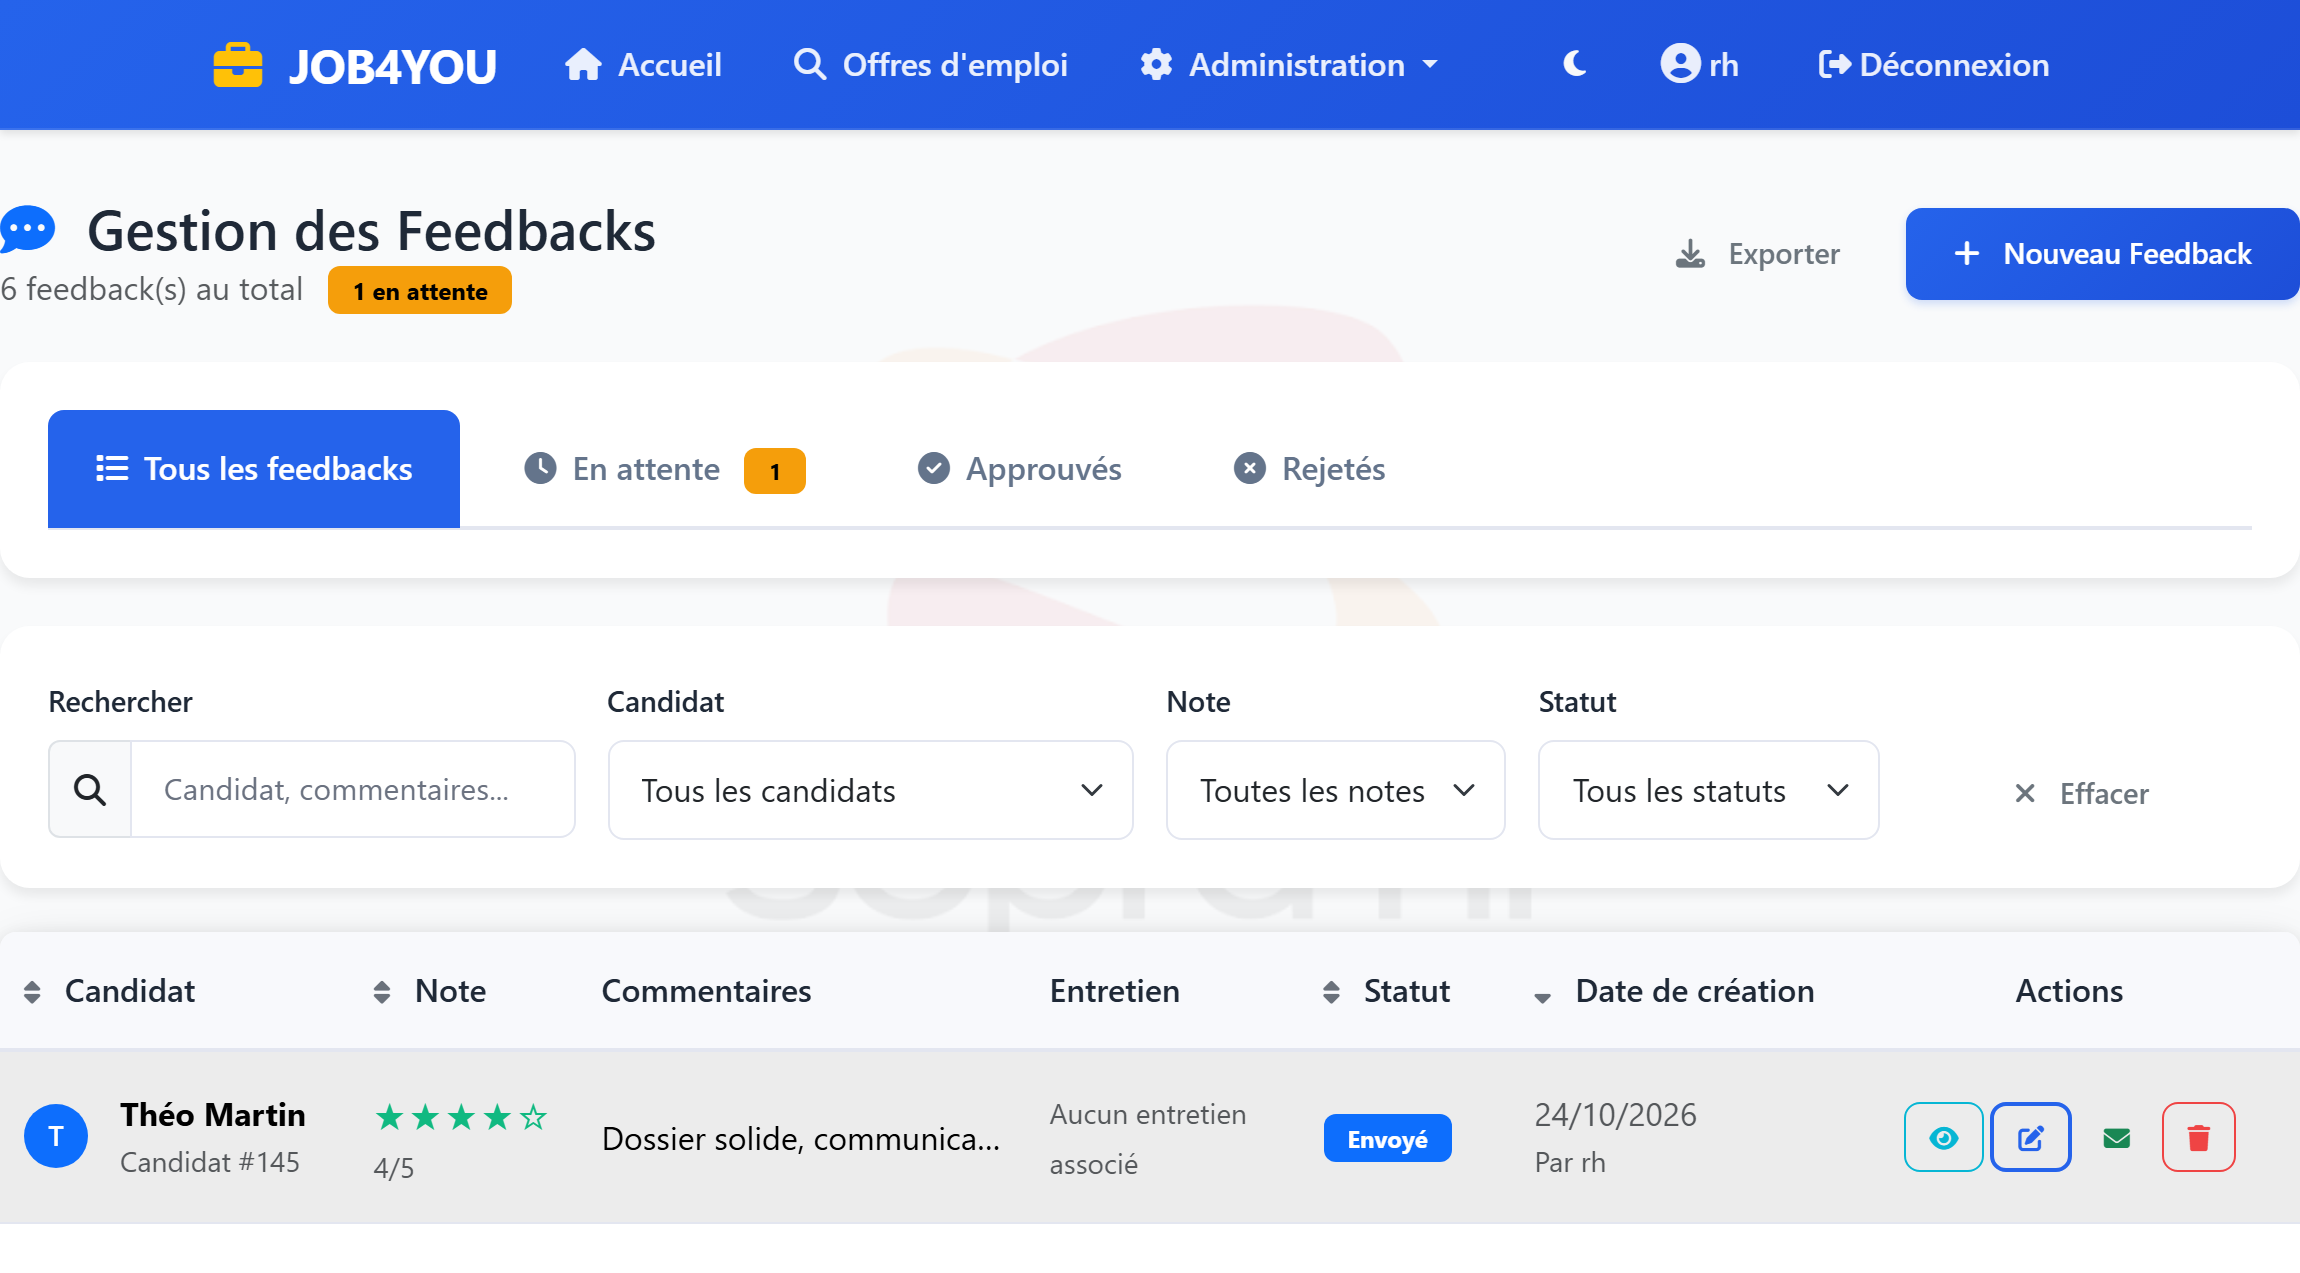
\includegraphics[width=0.98\linewidth, height=0.90\textheight, keepaspectratio]{fig4_12}
\caption{Gestion des feedbacks (espace RH)}
\label{fig_4_12}
\end{figure}
\clearpage
\end{landscape}

La figure~\ref{fig_4_12} centralise les retours saisis par les managers, notés de 1 à 5 étoiles et assortis d’un commentaire, avec une étape de validation par le RH avant transmission au candidat.

% figure 4.13
\setcounter{figure}{12}
\begin{figure}[!ht]
\centering
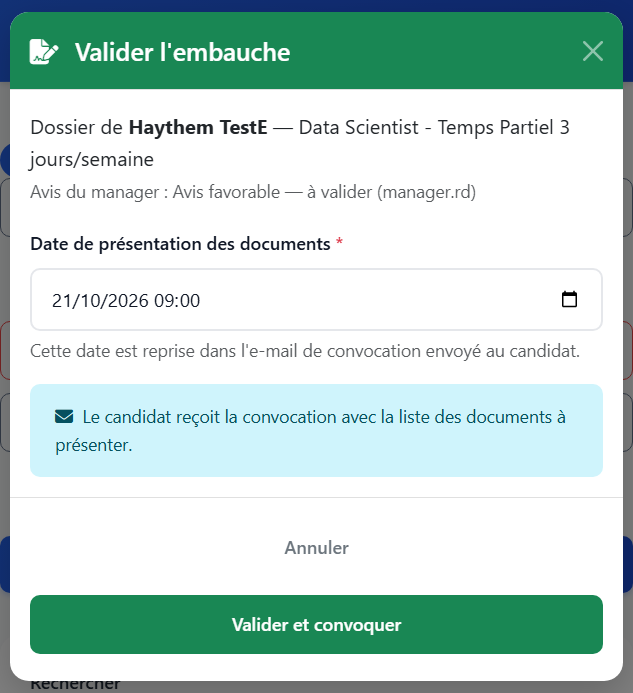
\includegraphics[width=\textwidth, height=0.80\textheight, keepaspectratio]{fig4_13}
\caption{Contreseing RH d’un avis favorable « Valider l’embauche »}
\label{fig_4_13}
\end{figure}

La figure~\ref{fig_4_13} présente la modale dans laquelle le RH contresigne l’avis favorable du manager avant l’embauche ; la date de présentation y est obligatoire, car elle alimente l’e-mail de convocation.

% figure 4.14
\setcounter{figure}{13}
\begin{figure}[!ht]
\centering
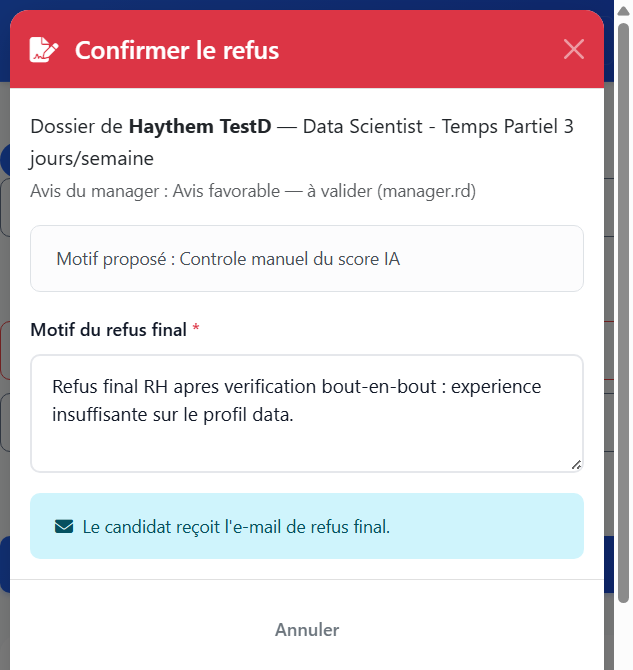
\includegraphics[width=\textwidth, height=0.80\textheight, keepaspectratio]{fig4_14}
\caption{Contreseing RH d’un refus proposé — modale « Confirmer le refus »}
\label{fig_4_14}
\end{figure}

La figure~\ref{fig_4_14} présente la modale « Confirmer le refus », où le RH contresigne le refus proposé par le manager. Le motif y est obligatoire, mais ne part pas dans l’e-mail au candidat, qui ne reprend que le nom et l’intitulé de l’offre. Le motif reste la trace humaine de la décision, journalisée dans l’audit.

\subsection{Espace Manager}
\label{sec_4_3_3}
% figure 4.15a
\setcounter{figure}{14}
% La capture originale fait 2664 x 1484 px : a cette taille, un texte de 22 px
% n'imprime qu'a 5,9 pt en paysage, ce qui est illisible sur projection comme sur
% papier. Elle est donc recadree en deux volets complementaires, chacun ramene a
% moins de 1760 px de large, soit 8,5 a 9,2 pt imprimes. Le ratio de chaque volet
% (3,0) rend le paysage nettement plus grand que le portrait (717 pt contre 484).
\begingroup\renewcommand{\thefigure}{4.15a}
\begin{landscape}
\pagestyle{lscape}
\begin{figure}[p]
\centering
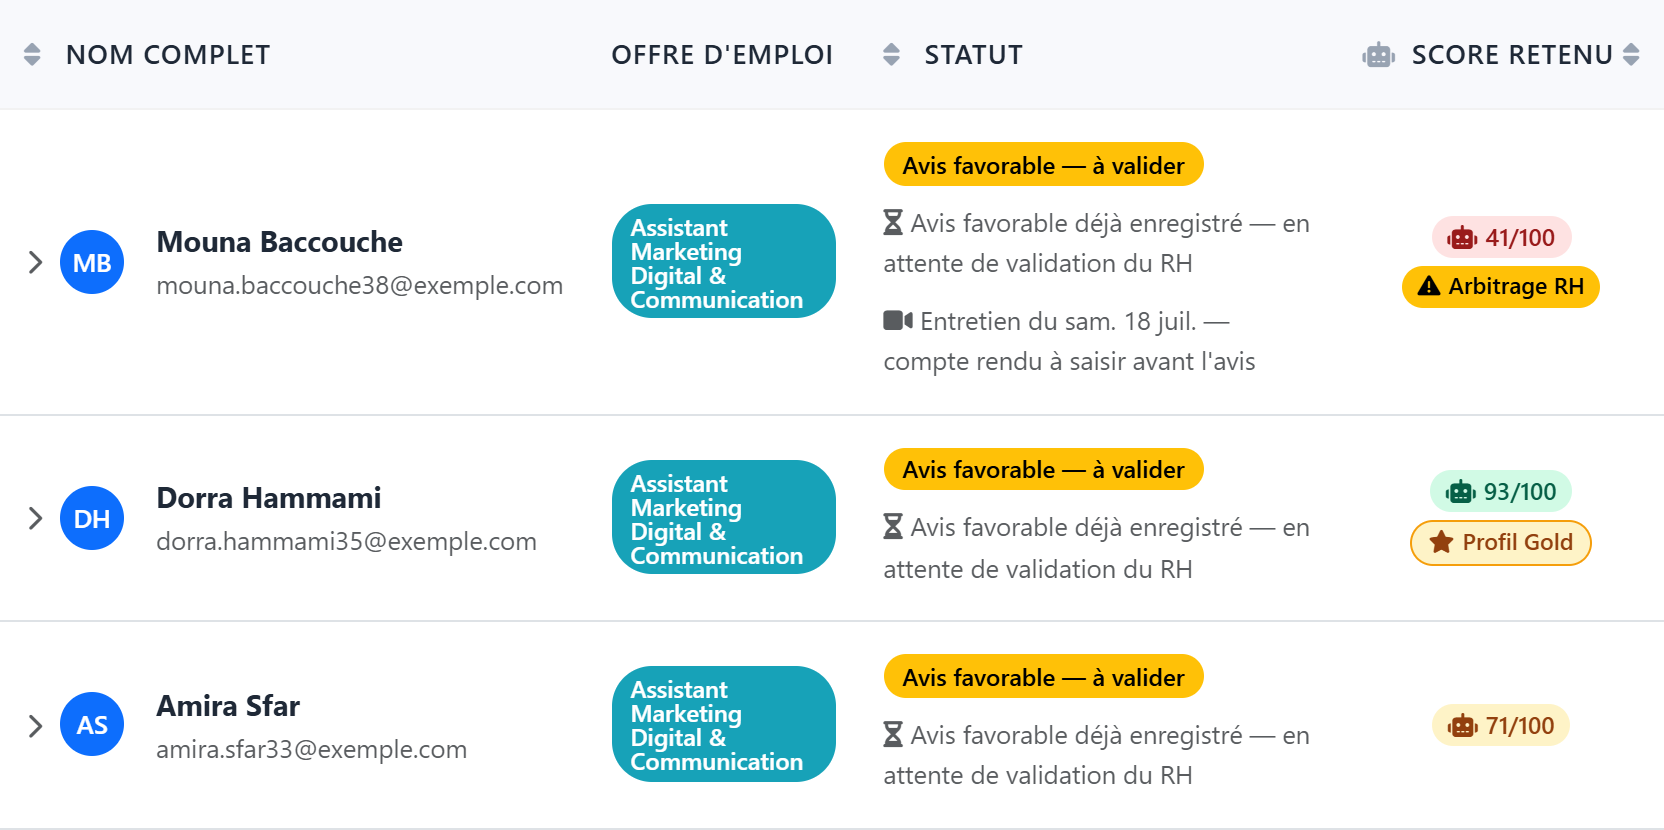
\includegraphics[width=0.98\linewidth, height=0.90\textheight, keepaspectratio]{fig4_15a}
\caption{Espace Manager — candidatures du périmètre : état d’avancement, avis du manager et score}
\label{fig_4_15a}
\end{figure}
\clearpage
\end{landscape}
\endgroup

% figure 4.15b
\setcounter{figure}{14}
\begingroup\renewcommand{\thefigure}{4.15b}
\begin{landscape}
\pagestyle{lscape}
\begin{figure}[p]
\centering
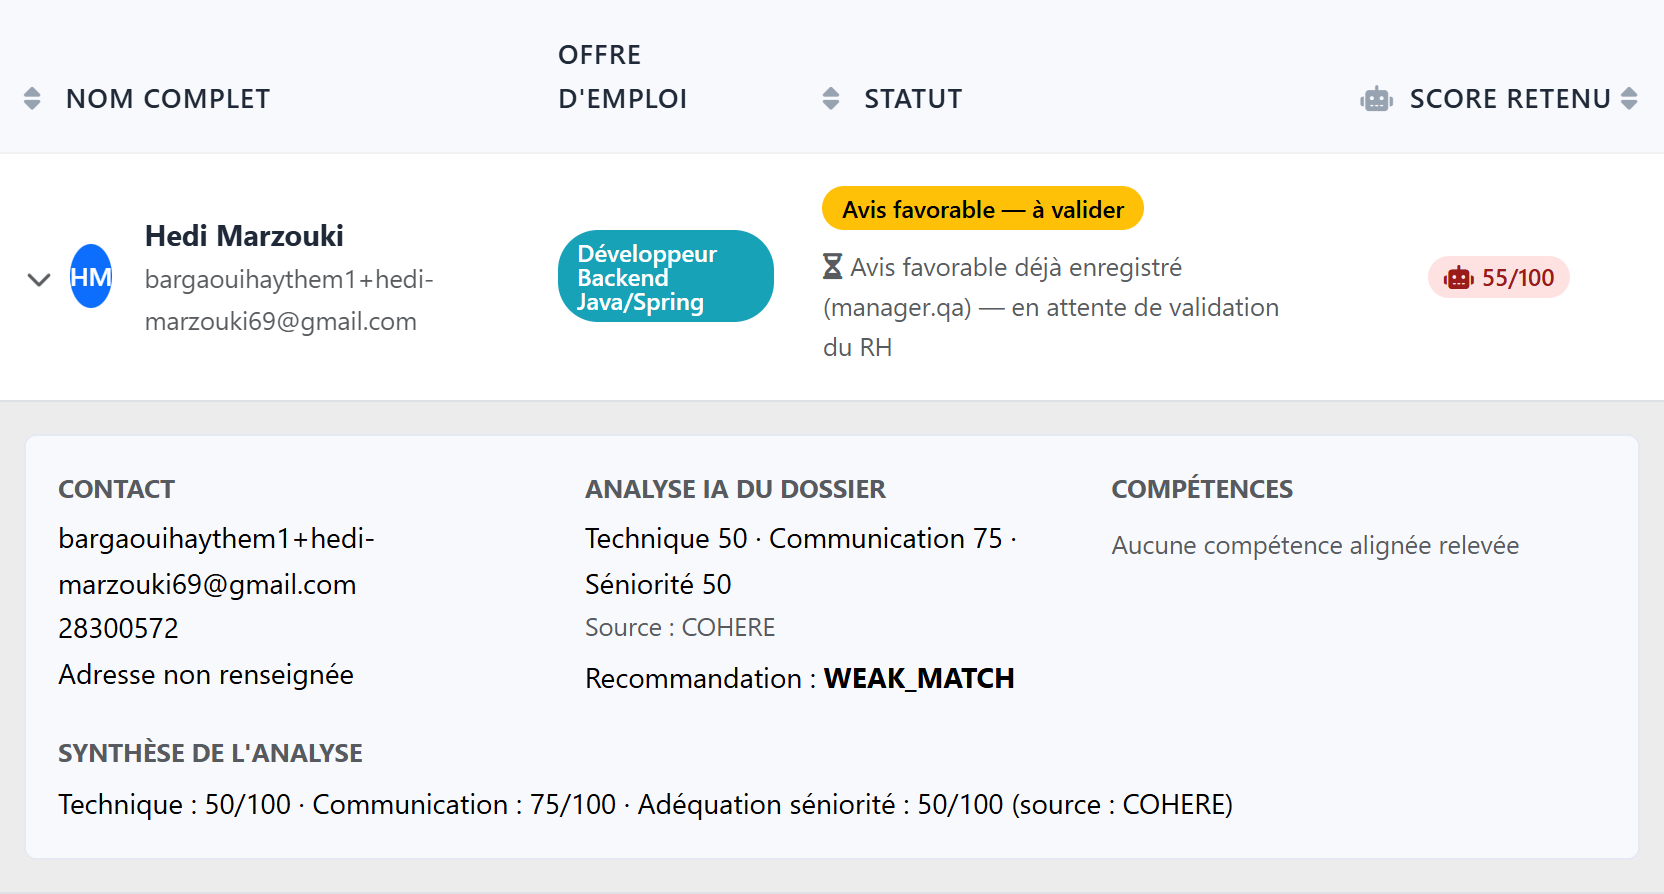
\includegraphics[width=0.98\linewidth, height=0.90\textheight, keepaspectratio]{fig4_15b}
\caption{Espace Manager — ligne dépliée : contact, analyse IA du dossier, synthèse et motif du statut}
\label{fig_4_15b}
\end{figure}
\clearpage
\end{landscape}
\endgroup

Un manager ne voit que les dossiers de son périmètre — le destinataire désigné par le RH, gelé sur la candidature (section 3.5.4) — à partir de leur entrée en évaluation technique. La figure~\ref{fig_4_15a} montre cette vue : chaque ligne porte le score retenu et le motif du statut — « Planifier l’entretien » tant que la date reste à fixer, « Avis favorable — à valider » quand le manager s’est prononcé — et se déplie sur le contact, l’analyse IA et la synthèse (figure~\ref{fig_4_15b}). Une étoile « Profil Gold », en lecture seule, y signale le profil de référence que le RH a validé pour cette offre ; le manager ne peut ni la poser ni l’enlever.

% figure 4.16
\setcounter{figure}{15}
% Capture recadree sur la seule carte « Prochains entretiens » : 1105 x 595 px,
% texte courant de 16 px imprime a 10,3 pt en paysage (boite 714 x 433 pt).
% L'encart « Rappels » et la liste « Entretiens passes », plus bas sur l'ecran,
% ne tenaient pas dans ce recadrage ; la grille et la fenetre de detail sont
% figures 4.16b et 4.16c.
\begin{landscape}
\pagestyle{lscape}
\begin{figure}[p]
\centering
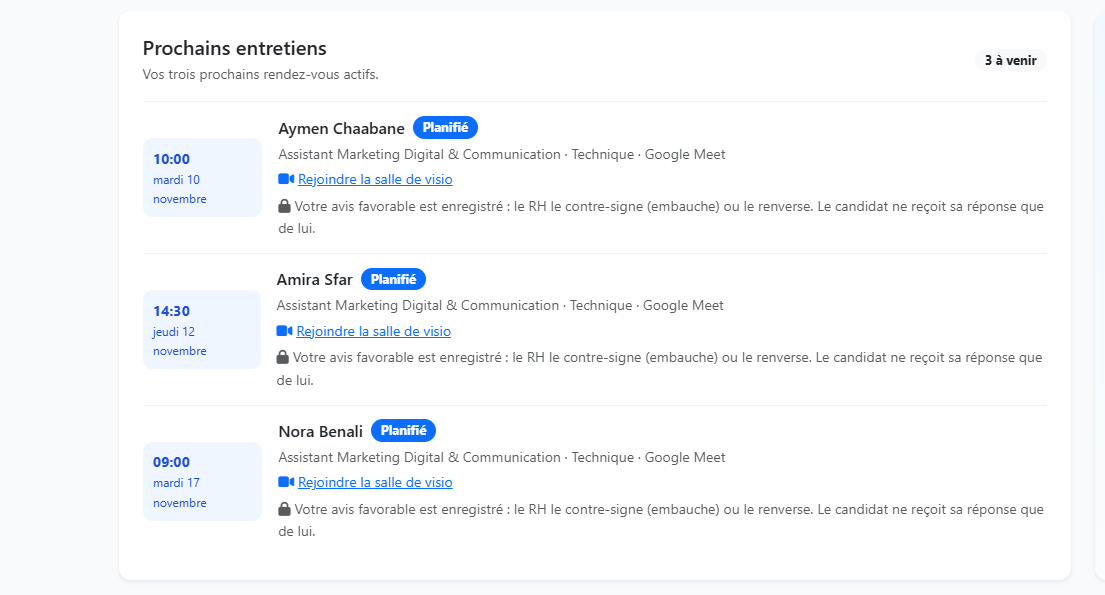
\includegraphics[width=0.98\linewidth, height=0.90\textheight, keepaspectratio]{fig4_16}
\caption{Espace Manager — page « Mon calendrier d’entretiens » : les trois prochains rendez-vous de l’intervieweur connecté}
\label{fig_4_16}
\end{figure}
\clearpage
\end{landscape}

La page « Mon calendrier d’entretiens » (figure~\ref{fig_4_16}) n’affiche que ce qui regarde l’intervieweur connecté : filtrage côté serveur sur sa seule identité, reprise du jeton, et même contrôle d’accès au dossier que pour la liste des dossiers. Elle n’est pas figée pour autant : le manager peut y marquer un entretien comme effectué et y reprendre un dossier encore instruit. Un encart « Rappels » annonce aussi un courriel deux heures avant chaque entretien, et une liste « Entretiens passés » ferme la page ; l’un et l’autre restent hors cadre.

Chaque carte porte l’heure, le jour, le candidat, le poste, le type d’entretien et le lieu, avec le badge d’état et le bouton « Rejoindre la salle de visio », qui n’apparaît qu’une fois le lien produit. Sous le bouton, une ligne dit où en est le dossier : « Votre avis favorable est enregistré : le RH le contre-signe (embauche) ou le renverse. Le candidat ne reçoit sa réponse que de lui. » Aucune commande de cet écran ne répond donc au candidat à la place du RH.

% figure 4.16b
\setcounter{figure}{15}
% Grille mensuelle recadree sur trois colonnes (mardi, mercredi, jeudi) et deux
% semaines : 596 x 256 px, chiffres de 14 px imprimes a 11,3 pt. La semaine
% complete a 1390 px de large ne tenait qu'a 7,0 pt, sous le plancher de 8,5 pt.
\begingroup\renewcommand{\thefigure}{4.16b}
\begin{figure}[!ht]
\centering
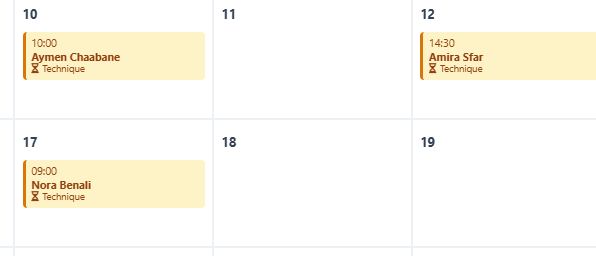
\includegraphics[width=\textwidth, height=0.80\textheight, keepaspectratio]{fig4_16b}
\caption{Grille mensuelle du calendrier manager — deux semaines de la vue de novembre, sur trois jours d’une semaine}
\label{fig_4_16b}
\end{figure}
\endgroup

La grille mensuelle (figure~\ref{fig_4_16b}) colore chaque créneau : l’ambre, marqué d’un sablier, signale un avis qui attend encore le contreseing du RH ; le gris, une décision déjà prise. Seules les colonnes mardi, mercredi et jeudi sont reproduites, les quatre autres jours de la semaine ne portant aucun rendez-vous dans cette base de démonstration. Le titre « Novembre 2026 » et les boutons de changement de mois restent également hors cadre.

% figure 4.16c
\setcounter{figure}{15}
% Fenetre de detail complete : 666 x 785 px, texte de 14 px. La page impose ici
% la hauteur (0,80 \textheight), la largeur d’impression descend a 445 pt,
% soit 9,4 pt imprimes.
\begingroup\renewcommand{\thefigure}{4.16c}
\begin{figure}[!ht]
\centering
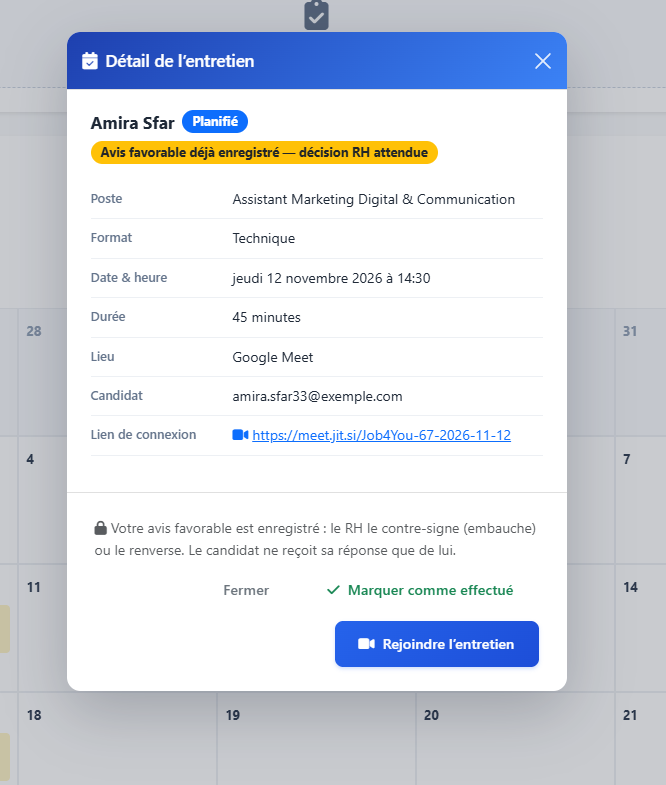
\includegraphics[width=\textwidth, height=0.80\textheight, keepaspectratio]{fig4_16c}
\caption{Fenêtre de détail d’un entretien : état de l’avis, informations du créneau, salle de visioconférence et commandes}
\label{fig_4_16c}
\end{figure}
\endgroup

Chaque événement ouvre une fenêtre de détail (figure~\ref{fig_4_16c}) : poste, format, date et heure, durée, lieu, candidat et lien de connexion. Le bandeau ambre y reprend l’état du dossier — « Avis favorable déjà enregistré — décision RH attendue » — et les commandes se limitent à « Fermer », « Marquer comme effectué » et « Rejoindre l’entretien ». Le lien est celui d’une salle créée par la plateforme à l’enregistrement de l’entretien ; il n’est actif que pendant le créneau, consulter le planning ne déclenche donc pas d’appel. Passé le créneau, le lien reste visible mais barré ; dossier clôturé, la carte affiche son état final (« Dossier clôturé : candidat embauché », « Dossier clôturé : refus validé par le RH ») sans bouton.

\subsection{Administrateur — comptes, paramétrage et traçabilité}
\label{sec_4_3_4}
% figure 4.17
\setcounter{figure}{16}
% Capture recadree sur les quatre premieres colonnes (identifiant, e-mail,
% roles, departement) et cinq lignes : 1545 x 446 px. La cinquieme colonne
% (famille de metier) etait deja coupee par le bord droit de l'ecran. Un texte
% de 20,6 px dans l'image vaut 9,6 pt imprimes (plancher 8,5 pt).
\begin{landscape}
\pagestyle{lscape}
\begin{figure}[p]
\centering
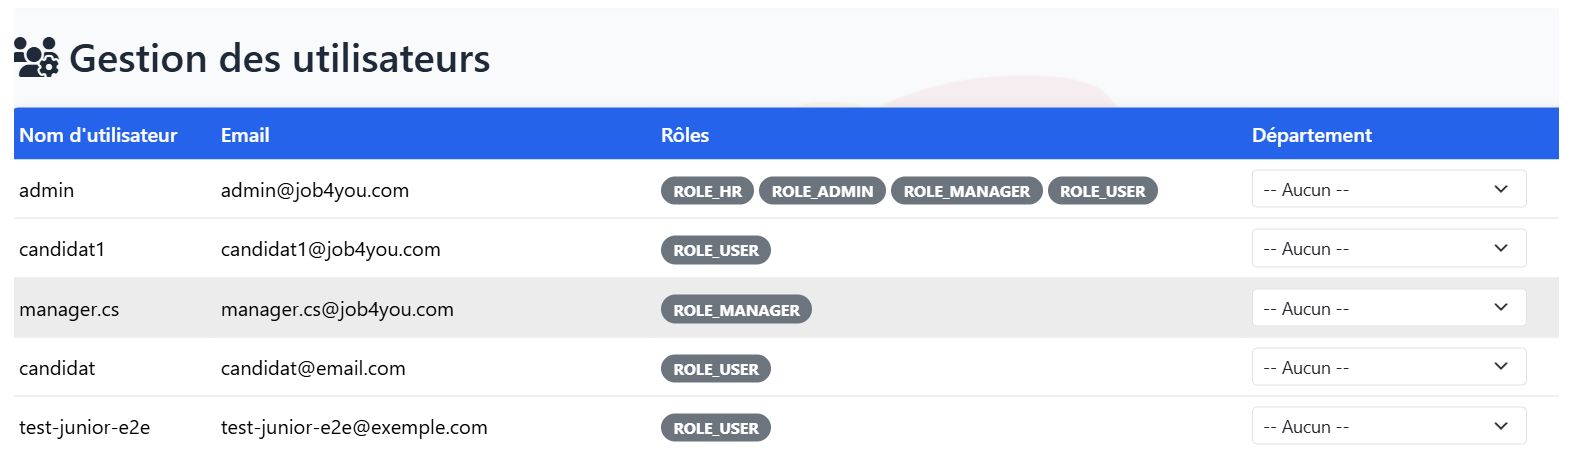
\includegraphics[width=0.98\linewidth, height=0.90\textheight, keepaspectratio]{fig4_17}
\caption{Gestion des utilisateurs et des rôles (espace Administrateur) --- partie gauche de l’écran}
\label{fig_4_17}
\end{figure}
\clearpage
\end{landscape}

L’écran de la figure~\ref{fig_4_17} permet à l’administrateur de gérer les comptes de la plateforme et leurs rôles, un même compte pouvant en cumuler plusieurs. Il définit aussi leur rattachement à un département ou, à défaut pour un manager, à une famille de métier.

% figure 4.18
\setcounter{figure}{17}
\begin{landscape}
\pagestyle{lscape}
\begin{figure}[p]
\centering
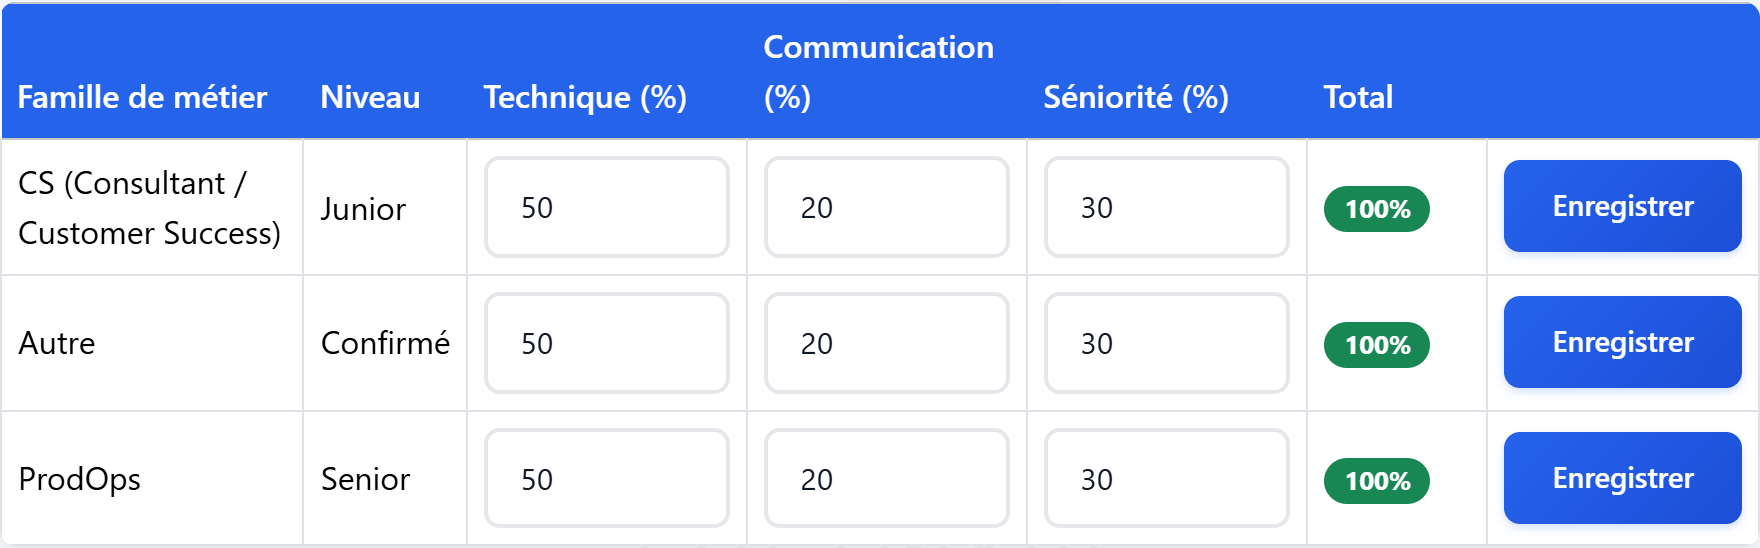
\includegraphics[width=0.98\linewidth, height=0.90\textheight, keepaspectratio]{fig4_18}
\caption{Paramétrage du scoring IA par famille de métier}
\label{fig_4_18}
\end{figure}
\clearpage
\end{landscape}

Réservé à l’administrateur et aux recruteurs, l’écran de la figure~\ref{fig_4_18} permet d’ajuster la pondération technique / communication / séniorité que l’agent IA utilise pour calculer un score. Le réglage porte sur chaque famille de métier et chaque niveau de séniorité ; une colonne de contrôle vérifie avant l’enregistrement que les trois poids totalisent bien 100 \%.

Le même écran héberge, sous ce tableau, une carte « Gold Set » : elle rejoue les vingt cas annotés dans le service de notation et affiche, pour chaque profil, le nombre de cas, le F1 mesuré au seuil en vigueur, le seuil recommandé et sa marge ; une proposition n’est applicable que si le contrôle qualité passe (section~\ref{sec_4_4_5}). Un recruteur peut y déposer un cas d’issue connue, anonymisé, qui vient enrichir le corpus sans modifier le socle.

% figure 4.19
\setcounter{figure}{18}
\begin{landscape}
\pagestyle{lscape}
\begin{figure}[p]
\centering
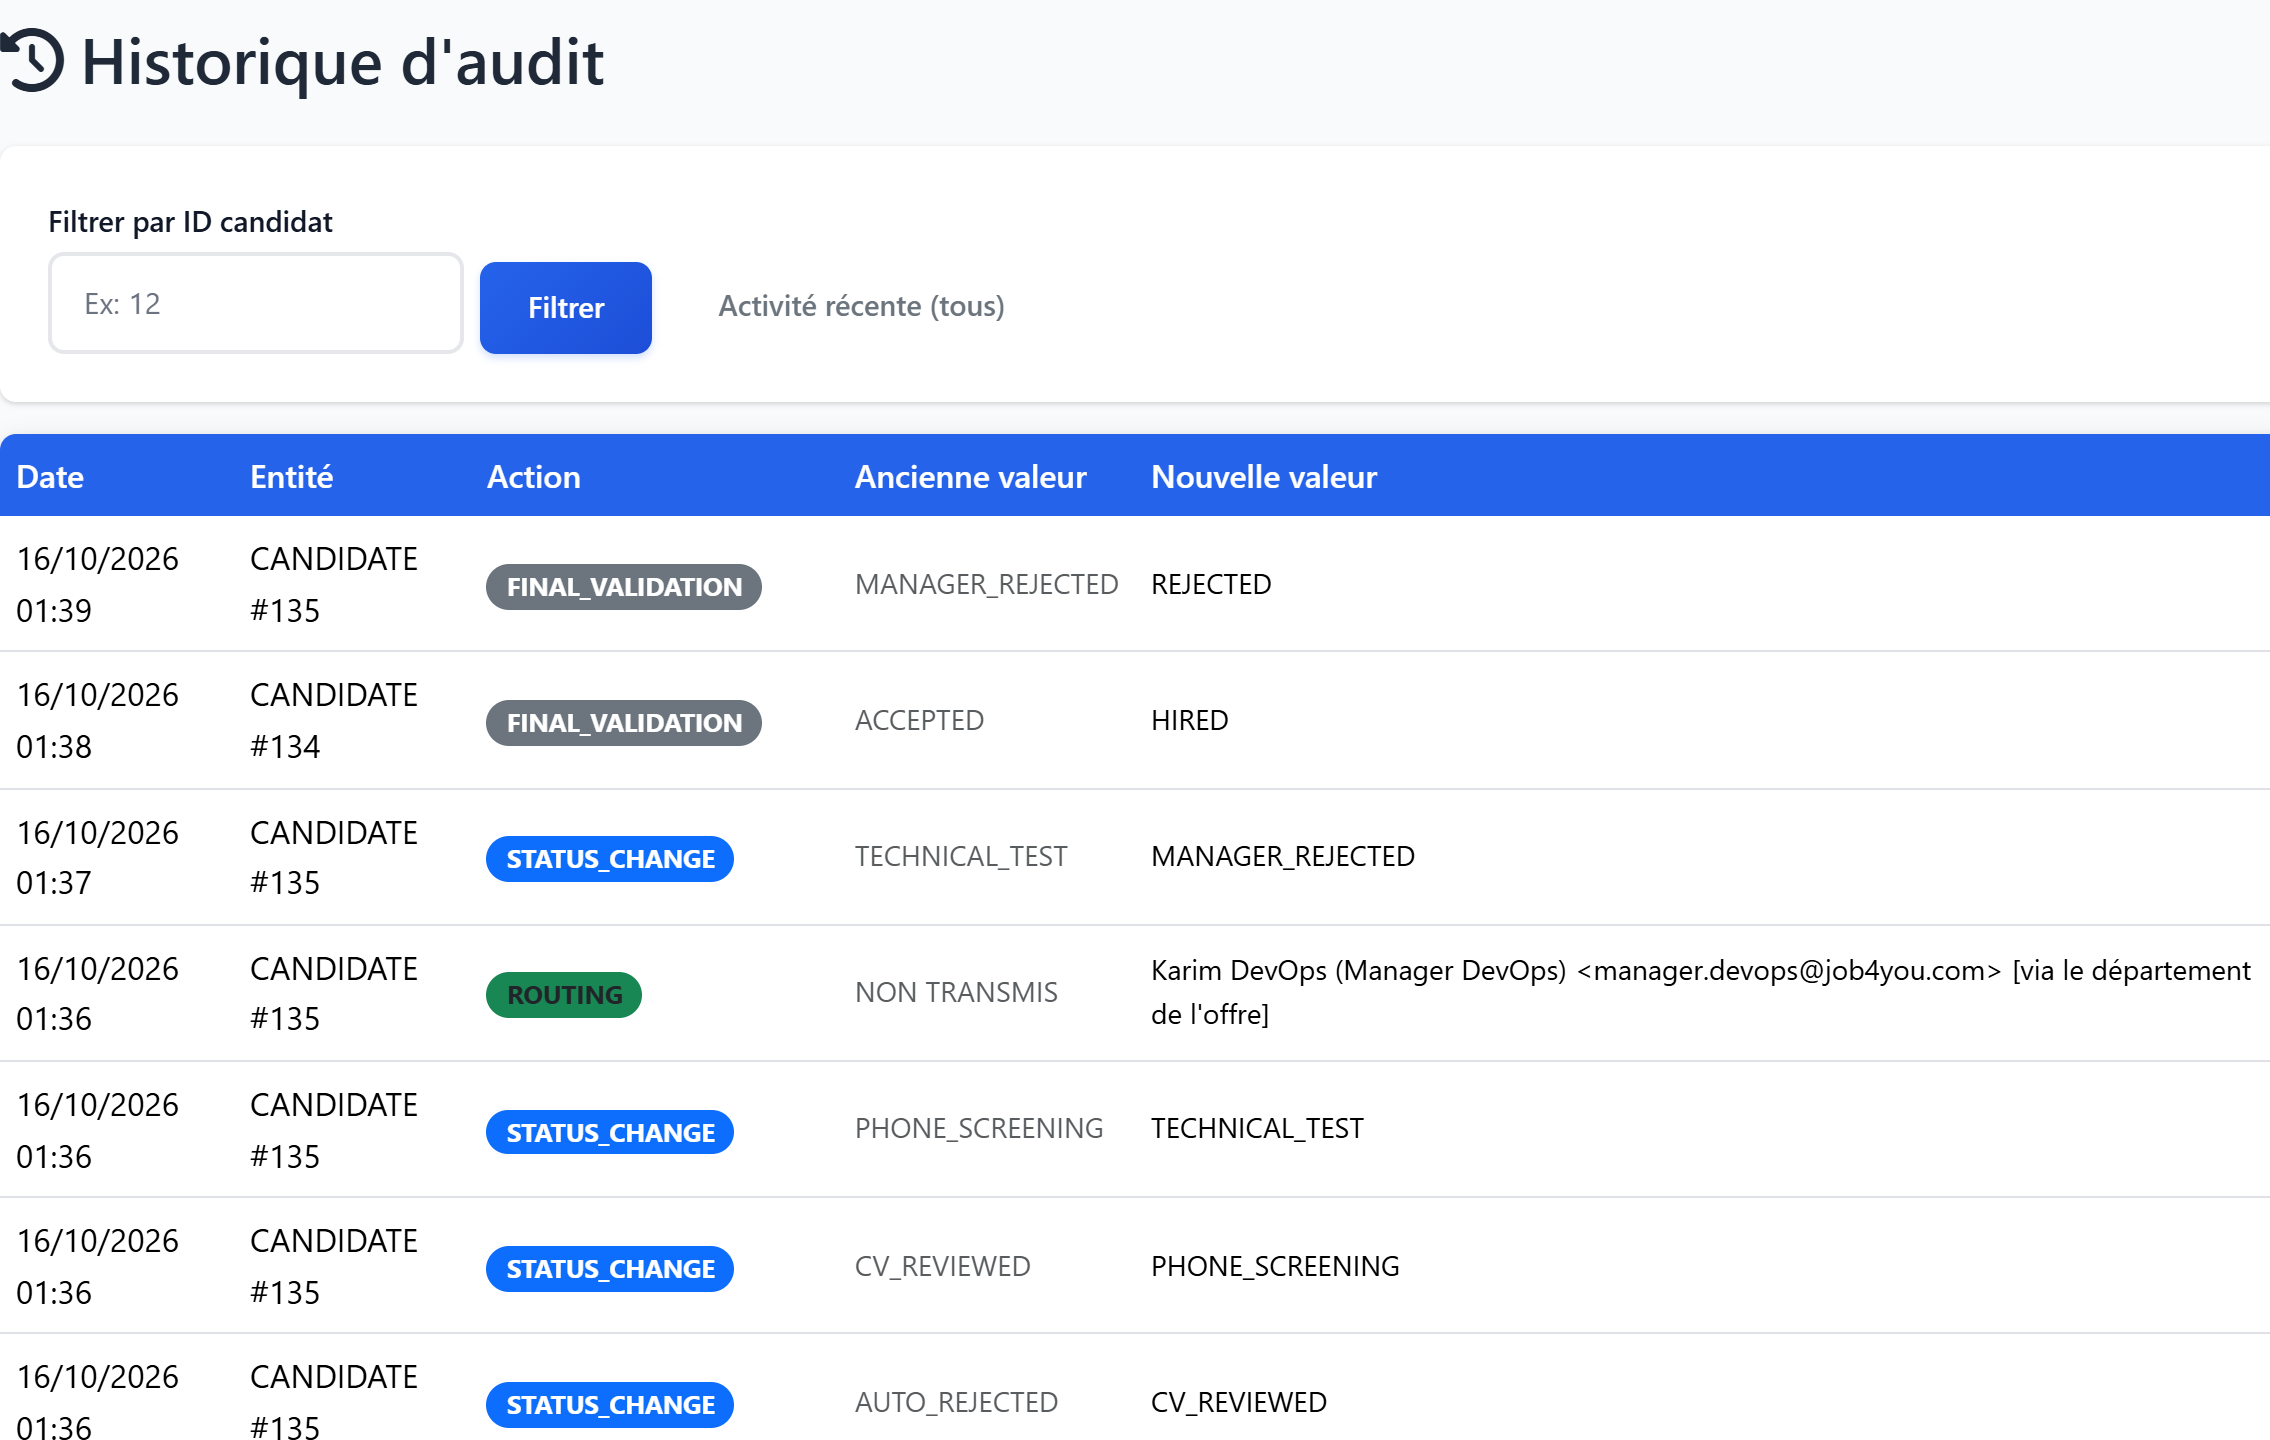
\includegraphics[width=0.98\linewidth, height=0.90\textheight, keepaspectratio]{fig4_19}
\caption{Historique d’audit}
\label{fig_4_19}
\end{figure}
\clearpage
\end{landscape}

L’historique d’audit de la figure~\ref{fig_4_19} trace les changements significatifs d’un dossier (statut, score, routage vers un manager, contreseing de la décision) avec la date, la nature de l’action et les valeurs précédente et nouvelle. La colonne « Effectué par », non reproduite sur le recadrage, nomme l’auteur de chaque écriture, humaine ou produite par les agents n8n.

\subsection{Automatisation n8n et notification du candidat}
\label{sec_4_3_5}
% figure 4.20
\setcounter{figure}{19}
\begin{landscape}
\pagestyle{lscape}
\begin{figure}[p]
\centering
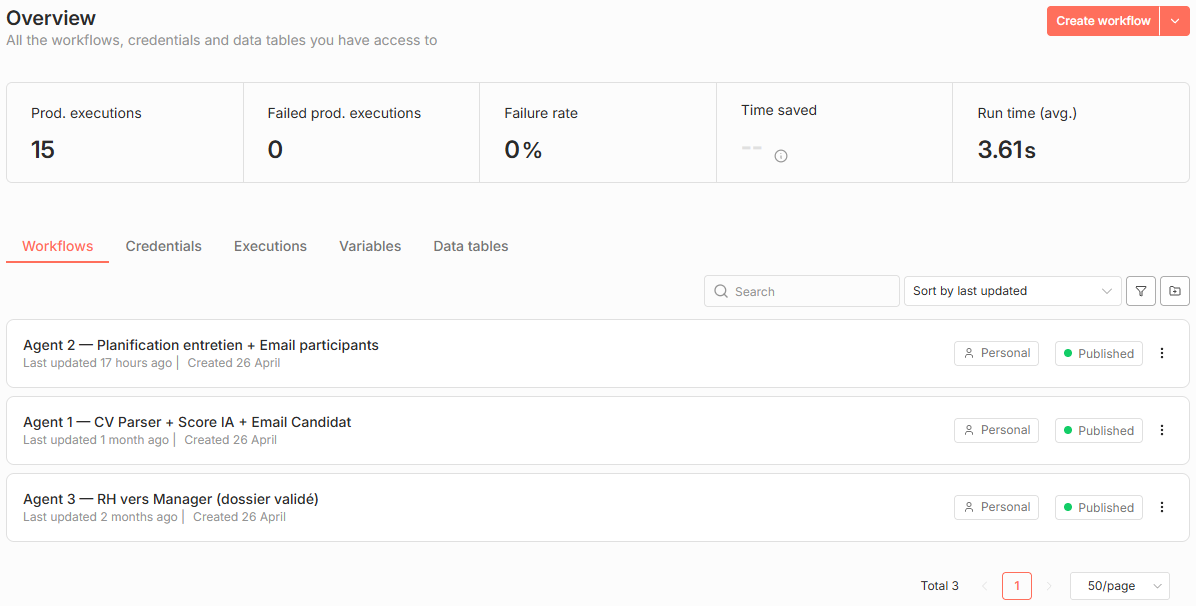
\includegraphics[width=0.98\linewidth, height=0.90\textheight, keepaspectratio]{fig4_20}
\caption{Console n8n — les trois flux d’automatisation publiés et leurs statistiques}
\label{fig_4_20}
\end{figure}
\clearpage
\end{landscape}

La chaîne a aussi été vérifiée dans la console n8n : la figure~\ref{fig_4_20} montre ses trois flux, tous publiés. Les compteurs du bandeau (119 exécutions, 30 en échec) viennent de l’agrégat interne, qui dénombre moins d’exécutions que la table (119 contre 154) mais converge sur les trente échecs. La mesure de référence reste celle de la table :
\begin{itemize}
\item 154 exécutions déclenchées par un événement, dont 124 abouties et 30 en échec ;
\item les trente échecs sont tous imputables au flux de planification et concentrés sur la période de calibration des 15 et 18 octobre : identifiants de messagerie refusés, échec de l’enregistrement du lien de visioconférence, accès aux variables d’environnement bloqué dans les nœuds ;
\item ces trois causes sont corrigées depuis, et aucun échec n’est postérieur au 18 octobre ;
\item durée moyenne d’une exécution réussie : 5,6 s, les plus lentes étant l’analyse du CV (6,0 s) et la transmission au manager (6,2 s), l’appel au service d’analyse et les envois de courriels s’exécutant en série ;
\item ces mesures relèvent d’un environnement local : l’échantillon ne vaut ni test de charge ni garantie de disponibilité.
\end{itemize}

% figure 4.21
\setcounter{figure}{20}
\begin{landscape}
\pagestyle{lscape}
\begin{figure}[p]
\centering
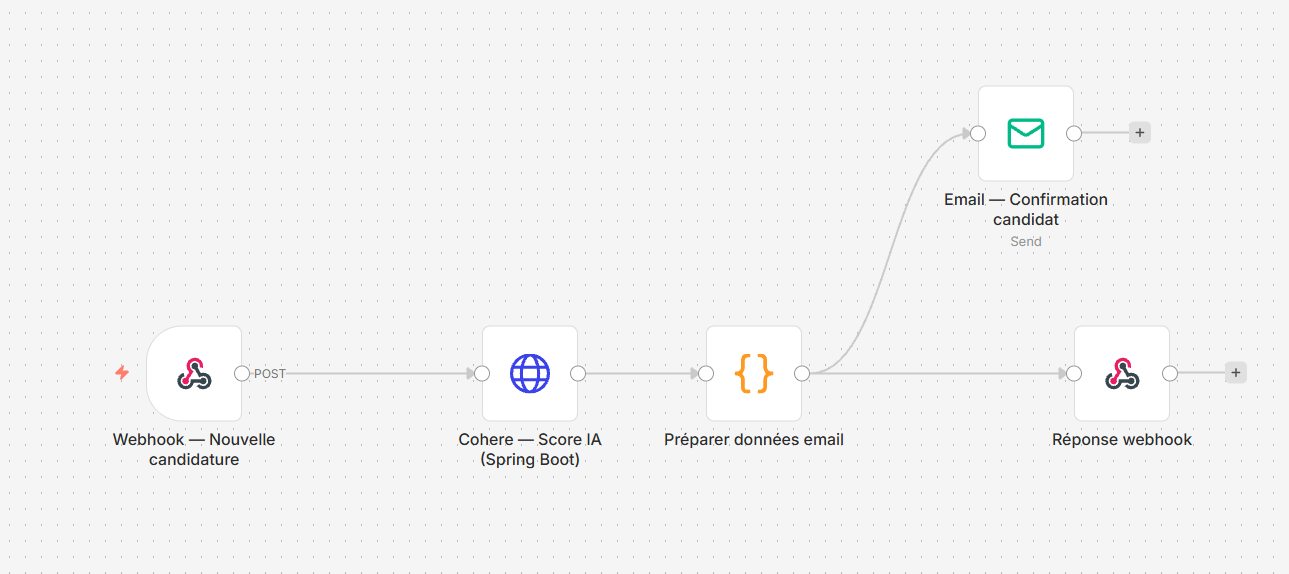
\includegraphics[width=0.98\linewidth, height=0.90\textheight, keepaspectratio]{fig4_21}
\caption{Flux n8n de l’Agent 1 — webhook de candidature, appel du scoring Cohere puis e-mail au candidat}
\label{fig_4_21}
\end{figure}
\clearpage
\end{landscape}

Le détail de l’Agent 1 (figure~\ref{fig_4_21}) confirme le découpage des responsabilités décrit au chapitre 3. Le webhook « Nouvelle candidature » reçoit l’événement émis par Spring Boot. Le nœud « Cohere — Score IA (Spring Boot) » rappelle le back-end, qui interroge réellement l’API de Cohere et persiste le score. « Préparer données email » alimente ensuite l’envoi de la confirmation au candidat.

% figure 4.22
\setcounter{figure}{21}
\begin{landscape}
\pagestyle{lscape}
\begin{figure}[p]
\centering
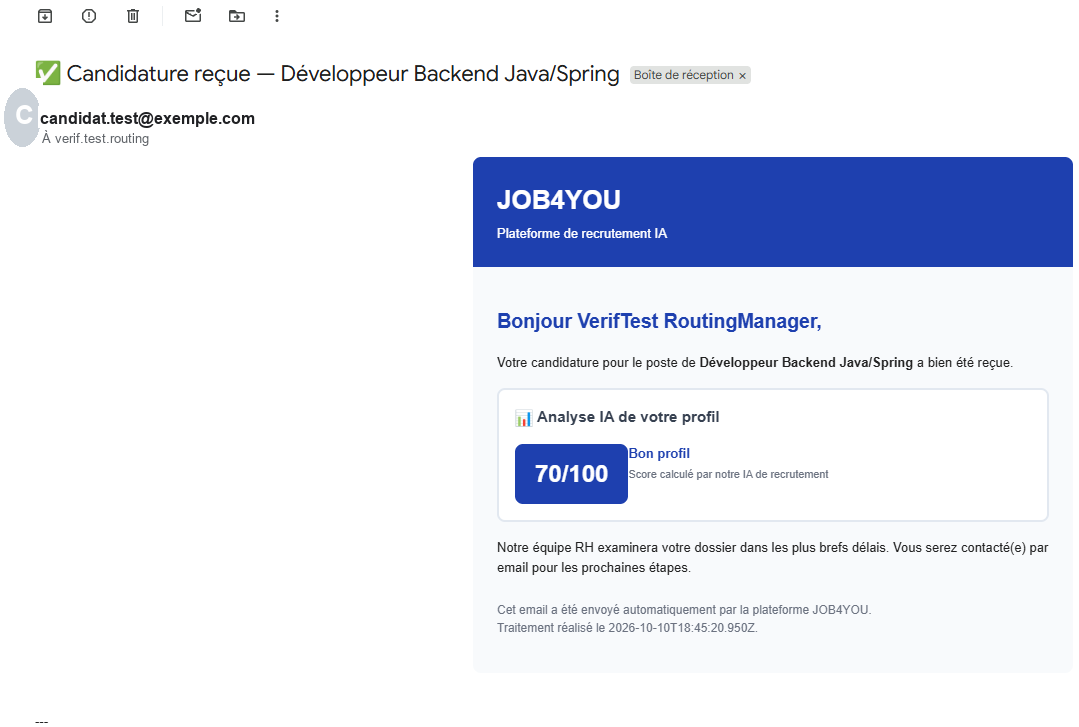
\includegraphics[width=0.98\linewidth, height=0.90\textheight, keepaspectratio]{fig4_22}
\caption{E-mail automatique de confirmation de candidature reçu par le candidat}
\label{fig_4_22}
\end{figure}
\clearpage
\end{landscape}

Côté candidat, la notification arrive bien dans sa boîte : la figure~\ref{fig_4_22} reproduit le message généré pour la candidature de la figure~\ref{fig_4_3} — accusé de réception nominatif, score obtenu et horodatage. Quand l’analyse n’a pas abouti, le bloc score laisse place à l’encart « profil en cours d’analyse » (section~\ref{sec_4_6}).

\section{Tests}
\label{sec_4_4}
\subsection{Tests unitaires (JUnit 5 / Mockito)}
\label{sec_4_4_1}
Au-delà des vérifications manuelles, la couche service et une partie de la couche controller sont couvertes par une suite automatisée écrite avec \logo{junit} JUnit 5 et Mockito \cite{ref16,ref24} et exécutée via Maven : 22 classes pour 264 méthodes, toutes exécutées sans échec. Dix-huit sont des tests unitaires purs : chaque service y est isolé par des doublons Mockito.

Ils couvrent quatre domaines :
\begin{itemize}
\item le dossier candidat, l’offre, l’aiguillage et le périmètre du manager, les propositions de département et la file d’attente d’automatisation avec sa clé d’idempotence ;
\item le scoring : profils de pondération, calcul du score, normalisation des compétences, lecture de la réponse du service d’analyse, compatibilité des offres et niveaux d’expérience ;
\item les notifications, les rappels et les entretiens ;
\item quatre tests de contrôleur, qui simulent une requête HTTP complète et vérifient les routes anonymes ainsi que l’accès au lien de visioconférence.
\end{itemize}

Ces tests verrouillent en particulier :
\begin{itemize}
\item la résolution des managers destinataires, son blocage lorsqu’aucun niveau n’en propose, et la journalisation d’un choix hors de la proposition ;
\item l’isolation stricte de la visibilité à la liste gelée sur le dossier ;
\item le calcul du score et ses seuils, avec l’orientation de tout score de la zone grise vers un arbitrage humain ;
\item la neutralisation d’une compétence que le CV nie explicitement ;
\item l’avancée du dossier à l’étape effectivement planifiée, et le refus du créneau qui en chevauche un autre à l’agenda du même intervieweur ;
\item l’arbitrage RH d’un dossier écarté d’office (confirmation motivée ou correction du score) sans seconde notification au candidat ;
\item l’envoi d’un unique courriel groupé à l’ensemble des comptes RH quand un avis attend le contreseing ;
\item la durée de vie d’un rappel : annulé si son entretien est reprogrammé, clôturé ou supprimé, purgé par le planifieur s’il est encore en file alors que l’entretien n’est plus à tenir — en plus des garde-fous de transition décrits au chapitre 3.
\end{itemize}

L’extrait ci-dessous, tiré de Candidate\allowbreak{}Service\allowbreak{}Test, illustre l’un des deux tests ajoutés pour valider le correctif décrit en section~\ref{sec_4_5_4} : il vérifie qu’un manager n’obtient, via get\allowbreak{}Candidates\allowbreak{}By\allowbreak{}Status(), que les candidats de son propre périmètre.

%% extrait reel de Candidate\allowbreak{}Service\allowbreak{}Test.java (lines 861-881)
\begin{lstlisting}[style=CodePFE]
@Test
@DisplayName("getCandidatesByStatus() ne renvoie à un manager que les candidats de son périmètre")
void shouldScopeGetCandidatesByStatusToCurrentManager() {
    Department rd = new Department("R&D", "R&D");
    rd.setId(1L);
    Department devops = new Department("4YOU", "4YOU");
    devops.setId(2L);

    Candidate inScope = candidateWithOffer(60L, "manager.rd@company.com", rd);
    Candidate outOfScope = candidateWithOffer(61L, "manager.devops@company.com", devops);
    User manager = makeManagerUser("manager_rd", "manager.rd@company.com", rd);

    authenticateAs("manager_rd", Role.ERole.ROLE_MANAGER);
    when(userRepository.findByUsername("manager_rd")).thenReturn(Optional.of(manager));
    when(candidateRepository.findByStatus(CandidateStatus.CV_REVIEWED))
            .thenReturn(List.of(inScope, outOfScope));

    List<CandidateResponse> result =
            candidateService.getCandidatesByStatus(CandidateStatus.CV_REVIEWED);

    assertThat(result).extracting("id").containsExactly(60L);
}
\end{lstlisting}

\subsection{Tests fonctionnels manuels}
\label{sec_4_4_2}
Chaque fonctionnalité développée a fait l’objet d’un test fonctionnel manuel directement dans l’application, couvrant à la fois le scénario nominal et les principaux cas d’erreur. Le tableau suivant synthétise les cas de test exécutés et leur résultat.

% tableau 4.1
\setcounter{table}{0}
{\captionsetup{labelsep=colon}
\renewcommand{\arraystretch}{1.25}\footnotesize
\begingroup%
\setlength{\tabcolsep}{4pt}%
\begin{longtable}{|P{0.302\textwidth}|P{0.540\textwidth}|P{0.104\textwidth}|}
\caption{Synthèse des tests fonctionnels réalisés}\label{tab_4_1}\\ \hline
\textbf{Cas de test} & \textbf{Résultat attendu} & \textbf{Résultat obtenu} \\
\hline
\endfirsthead
\multicolumn{3}{l}{\itshape Suite du tableau \ref{tab_4_1}}\\ \hline
\textbf{Cas de test} & \textbf{Résultat attendu} & \textbf{Résultat obtenu} \\
\hline
\endhead
\hline\endfoot
\hline\endlastfoot
Connexion avec identifiants valides & Connexion réussie, jeton JWT renvoyé & OK \\
Connexion avec mot de passe invalide & Erreur 401, accès refusé & OK \\
Accès à une route RH avec un compte Candidat & Refusé faute d’autorisation & OK \\
Publication d’une offre d’emploi par le RH & Offre créée et visible sur la page publique & OK \\
Dépôt d’une candidature avec CV & Candidature créée (statut « candidature déposée »), CV stocké et lié au dossier & OK \\
Analyse automatique du CV par l’agent IA & Score calculé, statut « CV validé » ou « écarté d’office » selon le seuil & OK \\
Avis manager sur un dossier non encore validé par le RH & Avis bloqué par le garde-fou métier & OK \\
Avis manager après validation RH & Avis enregistré (favorable ou refus proposé) et notifié au RH, sans e-mail au candidat & OK \\
Planification d’un entretien sur un dossier clos (refusé ou retiré) & Planification bloquée & OK \\
Notification par e-mail au candidat après la décision finale contresignée par le RH & E-mail reçu, contenu cohérent avec le statut & OK \\
Transmission RH $\rightarrow$ manager : l’aiguillage propose, le RH désigne le destinataire & Sans désignation : transmission refusée, dossier immobile ; le manager choisi est seul notifié ; choix hors proposition : journalisé & OK \\
Notification du manager à l’entrée en Test technique (après entretien téléphonique) & Le manager désigné est notifié à ce stade, pas avant & OK \\
Visibilité d’un manager sur un dossier d’un autre département & Aucun dossier hors de la liste gelée des destinataires n’est visible & OK \\
Retrait d’une candidature (statut « retiré ») & Le dossier quitte la liste active sans rechargement et reste filtrable & OK \\
Acceptation directe d’un candidat depuis « CV validé » (sans entretien téléphonique) & Transition refusée & OK \\
Chevauchement de deux entretiens d’un même intervieweur & Demande refusée ; le même jour reste possible & OK \\
Question du chatbot sur le statut réel d’une candidature & Réponse conforme aux données réelles en base, sans invention & OK \\
Demande du score IA ou de l’identité de l’intervieweur au chatbot & Refus poli, aucune donnée interne révélée & OK \\
Tentative d’injection de prompt sur le chatbot (« ignore tes instructions... ») & Le contexte système n’est pas divulgué, le rôle de l’assistant est conservé & OK \\
Appel du chatbot sans jeton d’authentification & Accès refusé & OK \\
Avis manager puis contreseing RH (« retenu » avec date / « refusé » motivé) & E-mail de convocation ou de refus motivé au candidat ; demande refusée si la date ou le motif manque & OK, vérifié le 14/10 en local \\
Transmission aux deux managers d’un dossier et relance d’un envoi échoué & Deux événements distincts, un par destinataire ; la relance émet une nouvelle clé et non un second silence & OK, vérifié le 14/10 en local \\
Arbitrage RH d’un dossier rejeté automatiquement par l’agent IA & Confirmation du refus (motivé, sans second e-mail au candidat) ou correction du score (retour à « CV validé ») ; demande refusée si le motif manque & OK, vérifié le 17/10 en local \\
\end{longtable}
\endgroup%
}
Les vingt-trois scénarios listés ont tous été exécutés avec succès ; cela ne vaut pas garantie globale : ces cas ne disent rien des chemins non exercés ni du comportement sous charge. La pertinence du scoring IA se mesure en section~\ref{sec_4_4_5}, et les temps de réponse de la section~\ref{sec_2_2_3} restent à valider en préproduction.

\subsection{Tests des API avec Postman et Swagger}
\label{sec_4_4_3}
J’ai testé isolément, à l’aide de Postman, l’ensemble des points d’entrée de l’API REST — en particulier les scénarios d’authentification, de contrôle d’accès par rôle et de gestion des erreurs (404, 400, 403). La documentation interactive Swagger, générée automatiquement à partir des annotations du code, m’a permis de vérifier la cohérence des contrats d’interface tout au long du développement.

\subsection{Vérification de bout en bout}
\label{sec_4_4_4}
J’ai aussi rejoué le parcours complet de bout en bout : candidature, analyse IA, validation RH, entretien, retour d’évaluation, avis du manager puis contreseing, chaque étape déclenchant l’e-mail attendu. Une vidéo commentée de ce parcours, courriels à l’appui, a été transmise à l’encadrant. Le fractionnement de la décision en deux niveaux est figé par des tests back-end (Candidate\allowbreak{}Service\allowbreak{}Test, section~\ref{sec_4_4_1}).

\subsection{Évaluation du matching sur un jeu de référence annoté (Gold Set)}
\label{sec_4_4_5}
Ces tests vérifient le fonctionnement de la plateforme, pas la pertinence du score. J’ai donc constitué un Gold Set \cite{ref21} de vingt curriculum vitæ synthétiques, inspirés de profils réalistes mais fictifs : aucun CV réel n’a été employé. Le corpus vit ensuite dans l’application même, et non dans un script d’évaluation à côté : la table \texttt{gold\_set\_cases} conserve, pour chaque cas, l’offre de calibration, la vérité terrain, le dernier score observé et son origine — \texttt{REFERENCE} pour le socle de vingt cas, qui ne bouge pas, \texttt{EXTENSION\_RH} pour un dossier dont l’issue est connue et qu’un recruteur ajoute après anonymisation. Une candidature réelle, même embauchée, ne rejoint jamais le corpus d’office : l’horloge de référence reste celle que l’humain a choisie.

Les vingt profils couvrent les trois familles visées : Développeur Backend Java/Spring (offre 115, sept cas), DevOps Engineer (offre 117, six) et Business Analyst (offre 122, sept).

Chaque cas porte une vérité terrain binaire, « pertinent » ou « non pertinent », arrêtée sur des critères objectifs (compétences indispensables, séniorité) et non d’après la sortie du modèle. Onze profils sont pertinents ; neuf sont volontairement hors cible (autre domaine, séniorité insuffisante ou outillage sans rapport).

L’écran « Gold Set » du paramétrage du scoring rejoue le corpus dans le service de notation lui-même — même extraction, même normalisation de compétences, même modèle — sur des dossiers éphémères qui n’entrent pas dans le pipeline. Le seuil de décision est balayé de 40 à 95 et la matrice de confusion est mesurée à chaque cran, globalement (tableau~\ref{tab_4_2}) et par profil.

% tableau 4.2
\setcounter{table}{1}
\begin{table}[!ht]
\centering
\caption{Matrice de confusion du Gold Set selon le seuil de décision}
\label{tab_4_2}
\renewcommand{\arraystretch}{1.25}\footnotesize
\setlength{\tabcolsep}{4pt}%
\begin{tabular}{|P{0.304\textwidth}|P{0.160\textwidth}|P{0.305\textwidth}|P{0.160\textwidth}|}
\hline
\textbf{Critère} & \textbf{Seuil = 50} & \textbf{Seuil = 60 (retenu)} & \textbf{Seuil = 70} \\
\hline
Vrais positifs (TP) & 11 & 11 & 11 \\
\hline
Faux positifs (FP) & 6 & 1 & 1 \\
\hline
Vrais négatifs (TN) & 3 & 8 & 8 \\
\hline
Faux négatifs (FN) & 0 & 0 & 0 \\
\hline
Précision & 64,7 \% & 91,7 \% & 91,7 \% \\
\hline
Rappel & 100 \% & 100 \% & 100 \% \\
\hline
F1-score & 78,6 \% & 95,7 \% & 95,7 \% \\
\hline
Exactitude & 70 \% & 95 \% & 95 \% \\
\hline
\end{tabular}
\end{table}
Réévaluation du 5 novembre 2026, vingt cas notés sans mode dégradé : au seuil de 60/100, dix-neuf bonnes décisions sur vingt, rappel de 100 \%, précision de 91,7 \% avec un seul hors cible retenu à tort (GOLD\_18, 74/100). À 50, cinq dossiers hors cible s’ajoutent et la précision retombe à 64,7 \% ; à 70, rien ne change.

La distribution justifie ce seuil : huit des neuf hors cible s’arrêtent à 57/100 ou moins, le plus faible profil pertinent atteint 71/100. Le seuil de 60/100 reste un réglage opérationnel, pas un optimum démontré ; le faux positif de GOLD\_18 lui subsisterait aux trois seuils, car seul le recruteur arbitre la proximité sémantique entre deux métiers voisins.

Le balayage est aussi mené profil par profil — la famille et le niveau portés par l’offre, le seuil étant stocké dans la table de pondérations de chaque profil (figure~\ref{fig_4_23}). Un seuil recommandé n’est appliqué que sous double condition : au moins quatre cas \texttt{REFERENCE} et un F1 mesuré à ce seuil d’au moins 90 \%. Le 5 novembre, les trois profils couverts obtiennent un F1 de 100 \% et recommandent 64/100 pour Consultant / Customer Success confirmé, 81/100 pour Product Ops senior — le seul déjà calibré et appliqué — et 67/100 pour les autres familles confirmées. La marge est la distance au score le plus proche du corpus : sept points pour les deux premiers profils, dix pour le troisième, donc aucun dossier ne frôle la frontière. Vingt cas ne verrouillent pas trois profils : deux restent au défaut 60/100.

% figure 4.23 - capture 900 x 512 px CSS (dpr 2), ratio 1,76 : la banniere de l ecran,
% deja dite dans le paragraphe, est coupee au recadrage. En paysage, l image tient alors en
% largeur (702 x 400 pt) et non plus en hauteur : 12,5 pt imprimes pour les 16 px CSS du
% tableau, 10,9 pt pour les mentions de 14 px, 10,0 pt pour les pastilles de seuil.
\setcounter{figure}{22}
\begin{landscape}
\pagestyle{lscape}
\begin{figure}[p]
\centering
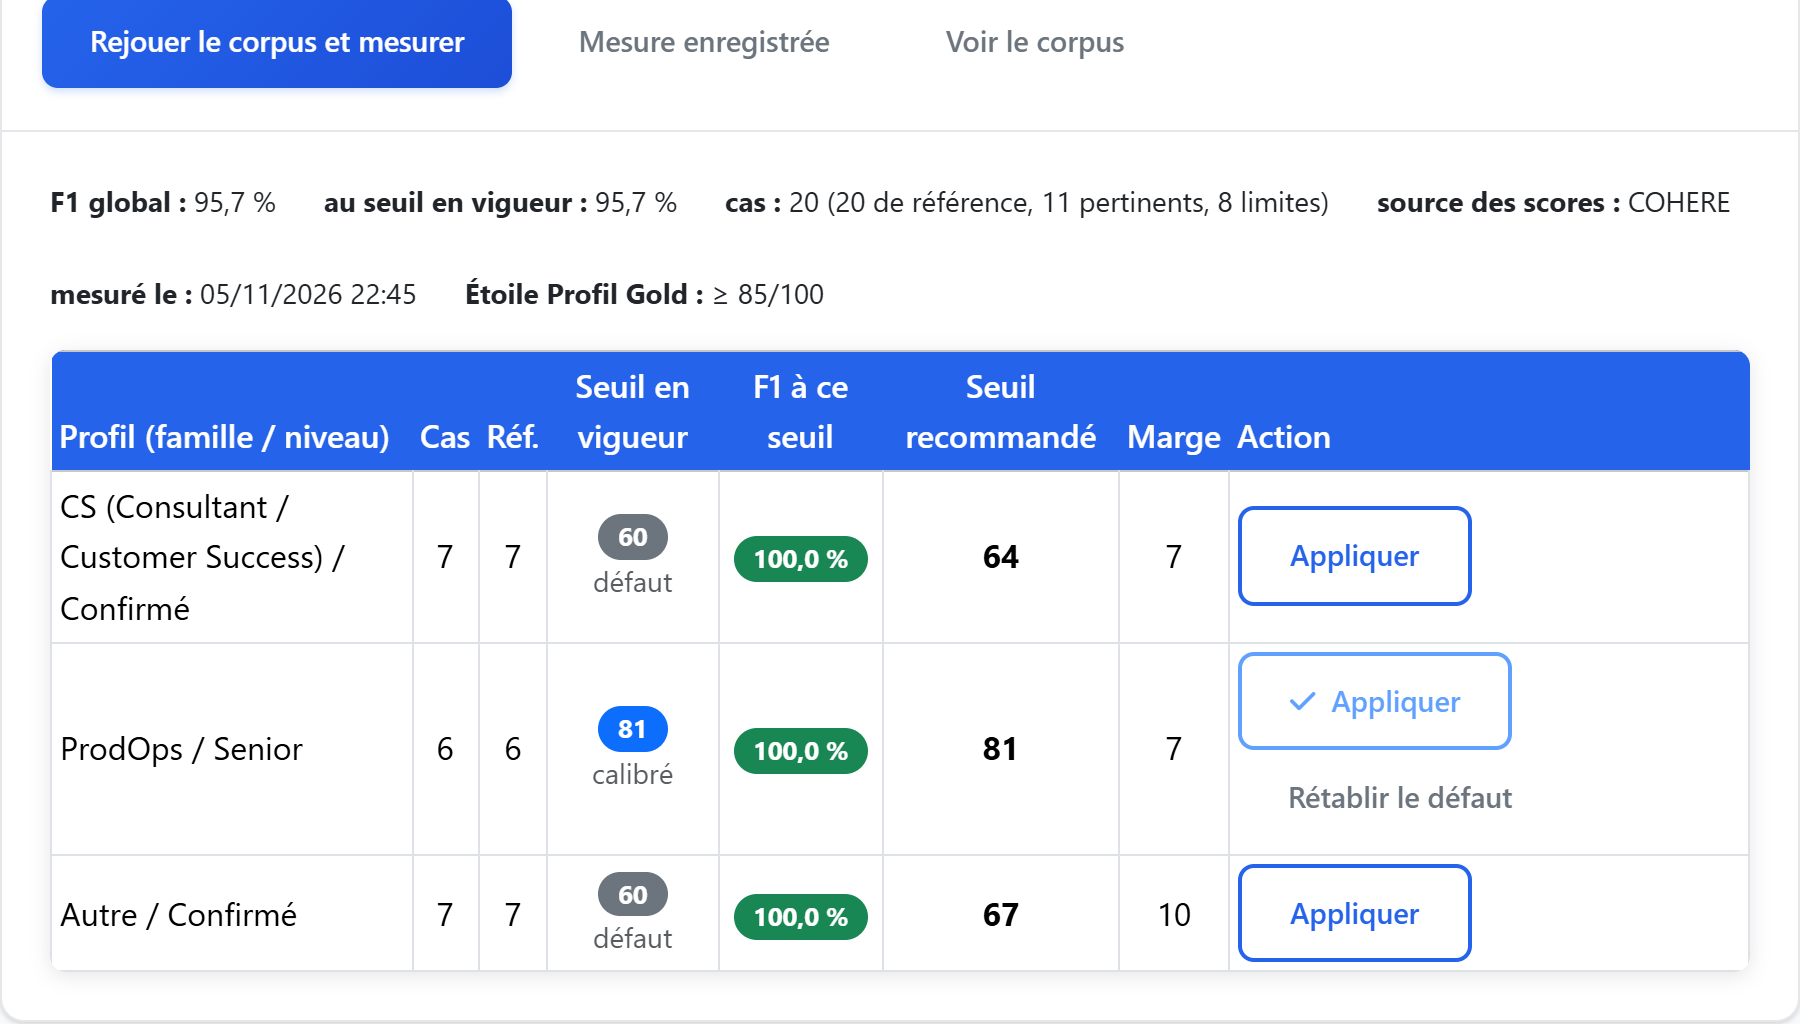
\includegraphics[width=0.98\linewidth, height=0.90\textheight, keepaspectratio]{fig4_23}
\caption{Paramétrage du scoring — écran « Gold Set » : rejouage du corpus et seuil recommandé par profil}
\label{fig_4_23}
\end{figure}
\clearpage
\end{landscape}


Le même corpus a été rejoué le 5 novembre 2026 par l’entrée réelle de l’application : vingt candidatures à part entière — confirmation par e-mail, agent de lecture, recalcul et transition de statut — relues une minute et demie plus tard. La matrice obtenue est identique à celle du tableau~\ref{tab_4_2}, les deux points d’entrée concordent (89 contre 89, 54 contre 54, 44 contre 44) et la plateforme a tranché seule : quinze dossiers conduits en revue technique, cinq écartés d’office, notation en 0,9 minute en médiane. Seize décisions sur vingt sont conformes à la vérité terrain, deux divergent, deux scores tombés en zone grise ont été transmis au RH sans que la machine tranche : c’est le comportement attendu du calibrage, pas une erreur du moteur.

Le corpus sert enfin d’étalon de confiance sur un dossier réel. Quand un score atteint la barre d’excellence (85/100) sur une analyse que le moteur ne signale ni incertaine ni dégradée, la fiche RH affiche une proposition « Profil Gold » : le recruteur la confirme ou l’écarte, et ni un recalcul ni le temps ne réveillent une décision déjà prise. Seule l’étiquette confirmée parvient au manager, qui lit alors, à côté du score retenu, un repère validé par un humain. Une candidature réelle n’alimente pour autant jamais le corpus d’évaluation : l’étiquette qualifie un dossier, le Gold Set étalonne le seuil.

Deux limites pèsent sur la comparaison. Les scores ne sont pas parfaitement reproductibles : GOLD\_18 est passé de 81 à 77 puis 74/100 selon les réponses du modèle, GOLD\_14 de 67 à 71/100 ; certains dossiers frôlent le seuil, et la zone d’incertitude existe pour cela. Vingt cas construits pour l’évaluation ne mesurent pas non plus la performance réelle : le Gold Set valide un mécanisme de décision et un calibrage de seuil, pas le suivi en production des faux positifs et faux négatifs constatés par les recruteurs.

\subsection{Validation humaine du score et explicabilité}
\label{sec_4_4_6}
Un moteur de présélection n’est fiable que s’il sait dire quand il ne l’est pas. Le service de scoring allume un drapeau d’arbitrage, avec un motif lisible, dans trois situations :
\begin{itemize}
\item texte extrait du CV trop court (moins de cinquante caractères : scan, image ou fichier dégradé) ;
\item score en zone grise, à cinq points au-dessous ou au-dessus du seuil du profil (55 à 65 pour le défaut de 60) ;
\item mode dégradé : le service d’analyse est indisponible ou inexploitable, et le score calculé localement porte l’origine « simulée ».
\end{itemize}
Le dossier signalé demande un arbitrage humain au lieu d’un tri automatique.

Les deux mécanismes se complètent : un score de 62 franchit le seuil et passe à « CV validé » avec le drapeau de zone grise ; un score de 57, sous le seuil mais signalé, y rejoint lui aussi un recruteur. Seuls GOLD\_04 et GOLD\_20 tombent dans cette bande (57/100), et aucun profil pertinent n’y descend, le plus faible atteignant 71/100 — la zone grise coûte donc du temps recruteur sans corriger d’erreur sur ce jeu.

L’explicabilité vient du service \texttt{Skill\allowbreak{}Normalization\allowbreak{}Service}, appelé avant le modèle de langage. Il harmonise les alias (k8s devient Kubernetes) et refuse les fusions abusives (Spring Boot n’est pas Spring Cloud). Il rend les compétences validées (\texttt{matchedSkills}) et manquantes (\texttt{missingSkills}), avec un recouvrement technique qui ne descend jamais sous 30/100. Une compétence citée sous négation (« aucune expérience des plateformes cloud managées ») n’est pas comptée comme acquise. Ces éléments alimentent les badges du détail de candidature (figure~\ref{fig_4_8}) et la synthèse \texttt{aiSummary} \cite{ref23}.

L’arbitrage est tracé : la correction manuelle, réservée aux rôles RH et Administrateur, exige un score de 0 à 100 et une justification non vide ; elle conserve \texttt{aiScore} et écrit \texttt{manualScore}, \texttt{manualScoreReason}, \texttt{manualScoreBy} et \texttt{manualScoreDate}. Le drapeau est réinitialisé, et une entrée « correction de score » est journalisée avec la valeur précédente, la nouvelle valeur et le motif.

Le statut est recalculé à partir du score effectif : un dossier en zone grise repart normalement dans le pipeline ; une correction sous le seuil le maintient « écarté d’office », sans nouvelle notification : le refus a déjà été envoyé par l’agent IA.

J’ai vérifié ce parcours de bout en bout : signalement, correction justifiée depuis un compte RH, puis ligne correspondante dans l’historique d’audit (figure~\ref{fig_4_19}). Le score de l’IA restant consultable, l’écart avec l’expertise humaine se mesure.

\section{Difficultés rencontrées et solutions apportées}
\label{sec_4_5}
Je détaille ici les principales difficultés rencontrées pendant le développement, représentatives des problèmes de ce projet.

\subsection{Notification incomplète des managers}
\label{sec_4_5_1}
L’aiguillage ne notifiait que le premier manager trouvé en base, sans lever d’erreur : la méthode retournait une adresse au lieu de la liste complète.

Chaque manager est désormais notifié individuellement, le courriel au candidat restant unique. Deux effets de bord du même genre ont été corrigés : la clé d’idempotence, identique pour tous les managers d’un dossier, était absorbée par la déduplication — elle intègre aujourd’hui l’adresse du destinataire ; et la destination dépendait d’attributs mutables de l’offre. La résolution hiérarchique, par ordre de priorité le manager désigné sur l’offre, le responsable du département, enfin la famille de métier, ne retient plus qu’une candidate, présentée dans la modale ; sans désignation explicite, l’envoi est bloqué et journalisé, et la destination est figée sur le dossier.

\subsection{Distinguer un avis manager d’une décision finale RH}
\label{sec_4_5_2}
Un seul statut couvrait les rejets RH et les rejets manager. La distinction passe par le cycle de vie : « refus proposé » pour l’avis en attente de contreseing, « refusé » pour le refus contresigné, « retenu » pour l’embauche validée ; motif et auteur complètent l’information.

\subsection{Cohérence des transitions de statut}
\label{sec_4_5_3}
Planifier un entretien ou trancher une décision n’a de sens que dans un état précis du dossier : sans garde-fou, on validait un candidat avant l’examen du RH. Une vérification côté back-end précède désormais chaque transition sensible, et l’interface reçoit un message d’erreur explicite plutôt qu’un échec silencieux.

\subsection{Filtrage incomplet des routes de lecture pour les managers}
\label{sec_4_5_4}
Le garde-fou de la section~\ref{sec_4_5_3} bloquait l’écriture hors périmètre, pas la lecture : liste, détail, recherche par nom et classement par offre ne filtraient rien. Un manager authentifié pouvait donc, en appelant directement l’API (l’interface n’expose pas ce chemin) , consulter des candidats d’un autre département.

La logique de périmètre est centralisée dans un service unique, qui lit la liste des destinataires gelée sur le dossier et non les attributs modifiables de l’offre ; aiguillage et visibilité partagent la même source. Des tests dédiés (section~\ref{sec_4_4_1}) figent ce comportement.

\subsection{Solliciter le manager au bon moment du processus}
\label{sec_4_5_5}
Le manager était notifié dès « CV validé », donc trop tôt : beaucoup de dossiers étaient encore écartés au pré-filtrage téléphonique. La notification est déplacée à l’entrée en Test technique, l’entretien téléphonique franchi ; le candidat reste informé de la présélection dès « CV validé », et la vue du manager n’affiche les dossiers qu’à partir du Test technique.

Le contrôle reste intact : la modale pré-sélectionne le manager proposé par l’aiguillage, l’envoi confirme le destinataire et l’état de chaque événement, et un échec se relance avec une clé renouvelée que la déduplication n’absorbe pas.

\subsection{Pertinence du matching Job idéal}
\label{sec_4_5_6}
Le matching inverse proposait du back-end à un profil DevOps. Le score ignorait l’intitulé de l’offre, et le jeu de résultats regorgeait de doublons. Combiner l’intitulé (60 \%) aux compétences (40 \%) et dédupliquer avant l’appel font que chaque profil (Java, DevOps, ProdOps, QA) ressort sur les offres qui lui correspondent.

\subsection{Traitement distinct des candidatures retirées}
\label{sec_4_5_7}
Une candidature retirée était confondue avec les rejetées dans les filtres, et la liste ne s’actualisait qu’après rechargement de la page.

Le retrait a désormais son propre filtre, dans la liste comme sur le tableau de bord, et tout changement de statut rafraîchit immédiatement la vue : le compteur est décrémenté sans rechargement. Ces candidatures restent consultables, comme les rejetées ; le candidat peut aussi retirer la sienne tant qu’elle n’est pas close, par une action qui lui est propre.

\subsection{Entretien téléphonique RH obligatoire avant acceptation}
\label{sec_4_5_8}
Le parcours RH autorisait l’acceptation directe d’un candidat depuis « CV validé » sans entretien téléphonique : la machine à états ne l’interdisait pas, alors que cet entretien est le premier filtre humain avant de solliciter le manager. La transition vers « avis favorable » a été retirée ; restent l’entretien, le refus et le retrait.

\subsection{Planification de l’entretien et statut du dossier}
\label{sec_4_5_9}
Planifier un entretien changeait le statut selon le type choisi, sans passer par le garde-fou de la section~\ref{sec_4_5_3} ni par le contrôle de périmètre : un entretien téléphonique sur un dossier déjà en phase technique suffisait à le faire régresser.

Supprimer tout effet de la planification rendait le manager incapable de faire avancer le dossier qu’on lui transmettait. Le contrôle est donc placé côté serveur : la planification propose l’étape correspondant au type retenu et la machine à états l’applique si elle l’autorise — une avancée refusée laisse le dossier en place, sans annuler l’entretien. Le manager n’a plus de case à cocher : l’agenda fait foi.

\subsection{Fiabiliser l’intégration Google Meet et le format des webhooks n8n}
\label{sec_4_5_10}
L’intégration Google Meet a échoué à trois reprises avant de tenir ; le tableau~\ref{tab_4_meet} liste chaque constat, sa cause et la correction.

% tableau 4.3
\setcounter{table}{2}
\begin{table}[!ht]
\centering
\caption{Défauts de l’intégration Google Meet et de la notification, leurs causes et leurs corrections}
\label{tab_4_meet}
\renewcommand{\arraystretch}{1.25}\footnotesize
\setlength{\tabcolsep}{4pt}%
\begin{tabular}{|P{0.215\textwidth}|P{0.360\textwidth}|P{0.360\textwidth}|}
\hline
\textbf{Défaut constaté} & \textbf{Cause} & \textbf{Correction} \\
\hline
Lien Meet fictif & Valeur produite par n8n, sans appel à l’API Google Calendar & Création réelle de l’événement avec sa conférence, puis extraction du lien \\
\hline
Routage cassé sans erreur & Le nœud Webhook imbrique le corps sous \texttt{body} alors que le workflow lisait les données à la racine & Lecture du champ \texttt{body}, corrigée aux trois endroits touchés \\
\hline
Lien vide et file encombrée & L’objet d’erreur du nœud Calendar se propageait : rappel refusé, cinq tentatives épuisées & Nœud d’extraction tolérant l’échec et condition d’envoi ; sinon avertissement journalisé et poursuite des deux e-mails \\
\hline
Rappel rejeté sans trace & En-tête d’authentification absent — \texttt{\$env} interdit dans un nœud d’appel — pendant que l’exécution affichait « success » & En-tête déclaré sur le nœud ; voie d’envoi vérifiée à part, réinitialisation à 22 h 37 et rappel J-1 à 23 h 00 contrôlés par réception sur la boîte de test \\
\hline
Quatre courriels identiques & Boucle sur les comptes RH, une copie indépendante par destinataire & Envoi groupé en un seul message portant la liste complète des adresses \\
\hline
Rappels périmés envoyés & Contenu conservé après reprogrammation ; entretien annulé ou clôturé sans purge & Annulation des rappels en attente avant reprogrammation, purge horaire avant tout envoi \\
\hline
\end{tabular}
\end{table}

Quatre précautions complètent le dispositif.
\begin{itemize}
\item un projet Google en mode « test » voit son jeton d’actualisation expirer après sept jours : le compte est reconnecté avant toute démonstration ;
\item sur indisponibilité passagère, le back-end met chaque envoi en file interne et le retente à délai croissant (5, 10, 20 puis 40 s, cinq tentatives) sans bloquer la requête initiale ;
\item la clé d’idempotence intègre l’adresse du manager : deux managers produisent deux envois, et une relance manuelle émet une clé neuve non absorbée par la déduplication ;
\item le lien n’est jamais inventé par l’agent : la plateforme crée une salle par défaut à l’enregistrement de l’entretien à distance, et le rappel de l’agent se borne à remplacer cette adresse par le lien de visioconférence, sans jamais l’effacer.
\end{itemize}
Le flux a été rejoué de bout en bout sur un entretien de démonstration, jusqu’à la reprise du même lien dans le calendrier du manager ; l’envoi des courriels reste délégué au service d’automatisation (section~\ref{sec_2_3_1}). Ces comportements sont fixés par les tests Notification\allowbreak Service\allowbreak Test et Reminder\allowbreak Service\allowbreak Test (section~\ref{sec_4_4_1}).

\subsection{Cloisonnement des données dans le chatbot candidat}
\label{sec_4_5_11}
Un utilisateur peut inciter un modèle de langage à révéler ce qu’il ne devrait pas, y compris son contexte. Première protection, dès la source : score et résumé de l’analyse, correction manuelle du RH, identité de l’intervieweur et notes internes sont absents du contexte envoyé à l’IA. Seconde protection, le message système : ne répondre qu’à partir de ce contexte filtré, ignorer toute instruction contraire glissée dans la question du candidat et ne jamais le reproduire mot pour mot.

Validé par trois tests manuels — demande du score, demande de l’identité de l’intervieweur, tentative d’injection de prompt (« ignore tes instructions précédentes… ») : l’assistant refuse sans rien divulguer. Ces tests réduisent le risque, sans garantie absolue face à toutes les injections.

\section{Protection des données et éthique de l’IA}
\label{sec_4_6}
La plateforme manipule identité, coordonnées, CV et évaluations des candidats. L’accès aux dossiers est contrôlé par rôle (tableau~\ref{tab_2_1}) : un manager ne voit que son périmètre, seuls le responsable RH et l’administrateur ont une vue d’ensemble ; les mots de passe sont hachés (section~\ref{sec_4_2_4}).

Le journal d’audit consigne chaque action sensible avec son auteur et son horodatage ; s’y ajoutent la limitation des tentatives de connexion et un garde-fou contre les redirections internes du point d’entrée de test. Reste à valider en production le contenu réel des fichiers déposés, pas la seule extension déclarée.

Le score est une aide à la présélection : selon la règle configurée, un score insuffisant déclenche un rejet automatique non précédé d’un examen humain, mais réversible par un responsable RH ou un administrateur. Deux issues : confirmer le refus après examen (motif obligatoire, sans seconde notification) ou le contester par une correction justifiée et journalisée. Les dossiers signalés pour arbitrage ne sont jamais rejetés automatiquement.

Cette conception limite le risque d’erreur ou de biais algorithmique sans équivaloir à une validation humaine de chaque décision, dans l’esprit du RGPD \cite{ref17,ref18} sur les décisions individuelles automatisées.

Ce dispositif comporte des limites qu’il convient d’assumer :
\begin{itemize}
\item la dépendance à un service d’analyse externe, Cohere, et à sa disponibilité ;
\item la sensibilité du score à la qualité et à la structure du CV fourni ;
\item le risque de biais inhérent à tout modèle statistique ;
\item et, à l’inverse, l’absence volontaire de décision entièrement autonome : chaque rejet automatique reste réversible par un opérateur humain.
\end{itemize}
Pour ne jamais bloquer un dépôt, un mode dégradé prend le relais si le service tombe. Le score est alors calculé par une heuristique locale (mots-clés, structure du texte) et son origine, réelle ou simulée, est consignée. Le message de confirmation reste générique : aucun score n’y figure.

Ces limites justifient une traçabilité complète et un examen humain des dossiers signalés ; les autres rejets automatiques ne sont pas validés au préalable. La conception intègre aussi diversité et inclusion, pour limiter le risque de discrimination d’une sélection automatisée \cite{ref19} ; les captures de la section~\ref{sec_4_3} utilisent des données fictives ou anonymisées.

Le chatbot (section~\ref{sec_4_5_11}) applique les mêmes principes : il ne s’appuie que sur les données du candidat connecté, dérivées côté serveur du jeton JWT et non d’un identifiant transmis par le client, et les champs internes restent exclus du contexte.

Sans étude de conformité, un rappel : le scoring passe par l’API de Cohere et l’assistant par celle d’OpenRouter (modèle \texttt{z-ai/glm-5.3-flash}, fixé par \texttt{openrouter.model}). Ces appels à des services tiers restent à encadrer — minimisation des données, information des candidats, clauses contractuelles, conditions de conservation à vérifier avant tout usage sur données réelles.

Aucune politique de conservation et d’effacement des données (CV, évaluations) n’est encore prévue : archivage, purge automatique et exercice du droit à l’effacement restent à définir et à outiller.

Un scoring en recrutement relève des principes européens encadrant les décisions individuelles automatisées \cite{ref17,ref18} et l’IA à « haut risque » \cite{ref20} : traçabilité renforcée, supervision humaine, documentation du modèle. Ces exigences sont partiellement mises en œuvre ici — surcharge manuelle justifiée, journal d’audit, arbitrage humain.

\section{Bilan des fonctionnalités réalisées}
\label{sec_4_7}
\begingroup
\setlength{\emergencystretch}{4em}
Le tableau suivant récapitule, par grand domaine fonctionnel, l’état d’avancement des développements à l’issue du projet.
\par\endgroup

% tableau 4.4
\setcounter{table}{3}
{\captionsetup{labelsep=colon}
\renewcommand{\arraystretch}{1.25}\footnotesize
\begingroup%
\setlength{\tabcolsep}{4pt}%
\begin{longtable}{|P{0.862\textwidth}|P{0.101\textwidth}|}
\caption{Bilan des fonctionnalités réalisées}\label{tab_4_3}\\ \hline
\textbf{Fonctionnalité} & \textbf{État} \\
\hline
\endfirsthead
\multicolumn{2}{l}{\itshape Suite du tableau \ref{tab_4_3}}\\ \hline
\textbf{Fonctionnalité} & \textbf{État} \\
\hline
\endhead
\hline\endfoot
\hline\endlastfoot
Authentification et gestion des rôles (JWT, RBAC) & Réalisée \\
Gestion des offres d’emploi (création, publication, expiration automatique) & Réalisée \\
Gestion des candidatures et des CV & Réalisée \\
Scoring IA des candidatures (API de Cohere) et paramétrage par famille de métier & Réalisée \\
Gestion des entretiens (planification, statuts, rappels, lien Google Meet réel généré automatiquement) & Réalisée \\
Gestion des retours d’évaluation (saisie, validation RH) & Réalisée \\
Routage automatique RH $\rightarrow$ manager par priorité, liste gelée sur le dossier & Réalisée \\
Notifications automatiques par e-mail (agents n8n) & Réalisée \\
Tableau de bord et pipeline de recrutement (Kanban) & Réalisée \\
Journal d’audit (traçabilité des actions) & Réalisée \\
Matching « Job idéal » (suggestion d’offres à partir d’un CV) & Réalisée \\
Entretien téléphonique RH obligatoire avant acceptation & Réalisée \\
Calendrier manager dédié (filtré sur l’intervieweur connecté) & Réalisée \\
Retrait de candidature en libre-service par le candidat & Réalisée \\
Assistant conversationnel candidat (chatbot IA via OpenRouter, connaissance des candidatures réelles et de la plateforme) & Réalisée \\
Gold Set de vingt CV annotés, rejoué et calibré dans l’application (écran d’étalonnage par profil) & Réalisée \\
Étiquette « Profil Gold » : proposition automatique, décision RH, repère visible du manager & Réalisée \\
Human-in-the-Loop : signalement des dossiers à arbitrer & Réalisée \\
Explicabilité du score : compétences validées / manquantes, source du score & Réalisée \\
Décision à deux niveaux : avis manager contresigné par le RH (convocation ou refus motivé) & Réalisée \\
\end{longtable}
\endgroup%
}
\section{Conclusion}
\label{sec_4_8}
Entre l’environnement de travail, les interfaces effectivement livrées, les tests menés et les difficultés qu’il a fallu résoudre en cours de route, ce chapitre reflète assez fidèlement le quotidien du développement de JOB4YOU. Reste maintenant à prendre du recul sur l’ensemble du projet — c’est l’objet de la conclusion générale qui suit.

        % ======== fin chap_04 ========
        \clearpage
        
        % ======== conclusion ========
\chapter*{Conclusion générale et perspectives}
\addcontentsline{toc}{chapter}{Conclusion générale et perspectives}
\markboth{Conclusion générale et perspectives}{}

En définitive, JOB4YOU est passé d’un besoin identifié en début de stage à une plateforme complète. Elle couvre tout le cycle de recrutement interne : publication d’une offre, réception des candidatures, analyse des CV par intelligence artificielle, planification des entretiens, retours des managers et décision finale.

Deux fonctionnalités la distinguent. Le matching inverse « Job idéal » suggère à un candidat les offres les plus compatibles avec son CV. Un assistant conversationnel lui laisse suivre ses dossiers en langage naturel, strictement borné à ses propres données. Des notifications par courriel et un tableau Kanban donnent aux RH et aux managers une visibilité en temps réel sur chaque dossier.

Techniquement, j’y ai approfondi Spring Boot et Spring Security côté serveur, Angular côté interface et la conception relationnelle sous PostgreSQL. J’y ai aussi mis en œuvre n8n et l’API de Cohere au service d’un processus métier concret, et travaillé la sécurité applicative : jetons d’authentification, contrôle d’accès par rôles.

La démarche conduite est itérative et incrémentale : huit sprints et quatre releases. J’ai également vérifié le comportement du seuil de décision du scoring sur un corpus de CV annotés à la main (Gold Set) et prévu, pour les cas limites, une validation humaine du score assortie d’une explication automatique des compétences retenues.

Au-delà du technique, ce stage m’a confronté aux contraintes réelles d’un grand groupe : sécurité, fiabilité, et un travail à rendre lisible pour des utilisateurs qui ne sont pas développeurs.

Plusieurs pistes d’évolution restent ouvertes pour poursuivre ce travail.
\begin{itemize}
\item \textbf{Fonctionnel} : un module d’analyse prédictive du taux de transformation des candidatures, une intégration plus poussée avec les plateformes d’emploi externes, et le report côté serveur du tri des candidatures RH, aujourd’hui limité à la page affichée.
\item \textbf{Tests} : la suite compte déjà 264 méthodes unitaires et de contrôleur (JUnit 5 / Mockito) ; lui restent à ajouter des tests d’intégration avec la base, des parcours de bout en bout (Playwright ou Cypress) et des tests automatisés des composants Angular.
\item \textbf{Évaluation de l’IA} : le jeu de référence de vingt profils, qui calibre désormais le seuil de décision depuis l’application, doit s’enrichir des cas d’issue connue que les recruteurs y déposeront anonymisés — seul moyen d’obtenir une mesure de performance en conditions d’exploitation.
\item \textbf{Industrialisation} : une chaîne d’intégration et de déploiement continus, puis un déploiement sur une infrastructure cloud, renforceraient la fiabilité et la scalabilité de la plateforme sur le long terme.
\end{itemize}

Les principales fonctionnalités prévues pour ce projet ont été développées et vérifiées à l’aide des scénarios décrits dans ce rapport : JOB4YOU répond aux besoins identifiés et tient son rôle sur toute la chaîne, de l’offre publiée jusqu’à la réponse au candidat.

Les objectifs de performance restent en revanche à mesurer. Plusieurs mesures de sécurité et de gouvernance doivent aussi être finalisées avant une mise en préproduction : validation du contenu des fichiers téléversés, politique de rétention et d’effacement des données, encadrement des transferts vers Cohere et OpenRouter.

Le système constitue donc un prototype fonctionnel, appelé à être industrialisé pour un déploiement chez Sopra HR Software Tunisie, plutôt qu’une solution dont l’aptitude à la production serait déjà démontrée. Cette expérience m’a permis de concevoir, sécuriser, tester et faire évoluer une solution logicielle complète.

        % ======== fin conclusion ========
        \clearpage

   
        \clearpage
        \printbibliography[title={Bibliographie}]
        % Pas d'annexes : le rapport s'arrete sur la bibliographie, comme dans le
        % rapport de PFE livre par l'ecole en exemple. annexes.tex, vide, etait
        % malgre tout inclus et imprimait une page sans contenu.
        \clearpage
    \backmatter
% \backmatter remise a zero du style de corps : a reposer ici, sinon les
% pages de suite de la bibliographie repartent avec le numero a droite.
\pagestyle{fancy}
        % ======== ./tpl/resume ========
%===== File containing the back cover of the document =====%
%                                                          %
% Copyright (C) ISI - All Rights Reserved                  %
% Proprietary                                              %
% Written by Med Hossam <med.hossam@gmail.com>, April 2016 %
%                                                          %
% @author: HEDHILI Med Houssemeddine                       %
% @linkedin: http://tn.linkedin.com/in/medhossam           %
%==========================================================%

%== It's advised to not modify the content of this file ===%
% To set your information, go to global_config.tex file    %
%==========================================================%

% Adaptation JOB4YOU : le resume (francais + anglais) depasse la page.
% Le bloc etait rendu dans une minipage, qui ne se coupe pas : le texte
% trop long etait purement et simplement retranche en bas de page. La
% minipage est donc remplacee par un paragraphe courant, qui pagine
% normalement. L'en-tete courant herite de la bibliographie, d'ou \markboth
% vide. Le bandeau du modele, lui, ne doit tomber que sur la toute derniere
% page, comme dans le rapport livre par l'ecole. Or \pagestyle{backcover} le
% posait aussi sur l'avant-derniere : le resume s'etale sur deux pages et le
% style s'applique a toutes celles qui suivent. Le bloc reste donc en style
% vide, et le style du modele n'est pose qu'avant \end{document}.
\pagestyle{empty}
\markboth{}{}
\newgeometry{bottom=15mm,left=15mm,top=17mm,right=15mm}

\begin{changemargin}{3mm}{0cm}
    \selectlanguage{french}

    \vskip1mm
    {\LARGE\textbf{Résumé}}
    \vskip1mm
    \begingroup
        \large
        \@frenchAbstract
    \endgroup
    \vskip1mm
    {\textbf{Mots-clés : }
        \begingroup
            \@frenchAbstractKeywords
        \endgroup
    }

    % Le resume et l'abstract partagent la derniere page : l'abstract
    % debordait de quelques lignes sur la page precedente, coupe en deux.
    % Une page par langue supprime la coupure sans couter de page (le
    % debord occupait deja cette page) et sans toucher au pied de page.
\end{changemargin}
% Nouvelle page puis descente d'un \baselineskip pour aligner le titre sur
% « Resume ». Deux hypotheses ont echoue, mesurees sur le build : la coupure
% par \clearpage seul (y=32,2) puis le meme \newgeometry qu'en tete du resume
% (y=32,2 encore, build du 04-11). La glue de tete de page est supprimee par
% TeX ; seul le \vspace* (forme etoilee) survit a cet endroit. La geometrie
% etant deja celle du resume, aucun \newgeometry n'est necessaire ici.
\clearpage
\vspace*{\baselineskip}
\begin{changemargin}{3mm}{0cm}

    \selectlanguage{english}

    \vskip1mm
    {\LARGE\textbf{Abstract}}
    \vskip1mm
    \begingroup
        \large
        \@englishAbstract
    \endgroup
    \vskip1mm
    {\textbf{Keywords : }
        \begingroup
            \@englishAbstractKeywords
        \endgroup
    }
\end{changemargin}

        % ======== fin ./tpl/resume ========

% Le style du modele ne se pose qu'ici : \thispagestyle vise la page en cours
% de composition, c'est-a-dire, a cet endroit, la derniere page du document.
\thispagestyle{backcover}

\end{document}
